%%%%%%%%%%%%%%%%%%%% book.tex %%%%%%%%%%%%%%%%%%%%%%%%%%%%%
%
% sample root file for the chapters of your "monograph"
%
% Use this file as a template for your own input.
%
%%%%%%%%%%%%%%%% Springer-Verlag %%%%%%%%%%%%%%%%%%%%%%%%%%`'


% RECOMMENDED %%%%%%%%%%%%%%%%%%%%%%%%%%%%%%%%%%%%%%%%%%%%%%%%%%%
\documentclass[envcountsame,envcountchap, openany]{mysvmono}
\usepackage[margin=1in]{geometry}
\usepackage[T5]{fontenc}

\usepackage[utf8]{inputenc}
\usepackage{amsmath}
\usepackage{amssymb}
\setlength{\parindent}{0em}
\setlength{\parskip}{1em}
% choose options for [] as required from the list
% in the Reference Guide, Sect. 2.2

\usepackage{makeidx}         % allows index generation
\usepackage{graphicx}        % standard LaTeX graphics tool
                             % when including figure files
\usepackage{multicol}        % used for the two-column index
\usepackage[bottom]{footmisc}% places footnotes at page bottom
% etc.
% see the list of further useful packages
% in the Reference Guide, Sects. 2.3, 3.1-3.3

\makeindex             % used for the subject index
                       % please use the style svind.ist with
                       % your makeindex program

\usepackage{cite,url,bm,hyperref}
\usepackage{hyperref}
\hypersetup{
    colorlinks=true,
    linkcolor=blue,
    filecolor=magenta,
    urlcolor=blue,
}

%%%%%%%%%%%%%%%%%%%5
\usepackage{listings}
\usepackage{color}

%New colors defined below
\definecolor{codegreen}{rgb}{0,0.6,0}
\definecolor{codegray}{rgb}{0.5,0.5,0.5}
\definecolor{codepurple}{rgb}{0.58,0,0.82}
\definecolor{backcolour}{rgb}{0.95,0.95,0.92}


\usepackage{courier}

%Code listing style named "mystyle"
\lstdefinestyle{mystyle}{
  backgroundcolor=\color{backcolour},   commentstyle=\color{codegreen},
  keywordstyle=\color{magenta},
  stringstyle=\color{codepurple},
  basicstyle=\footnotesize,
  breakatwhitespace=false,
  breaklines=true,
  captionpos=b,
  keepspaces=true,
  numbers=left,
  numbersep=5pt,
  showspaces=false,
  showstringspaces=false,
  showtabs=false,
  tabsize=2,
  basicstyle=\footnotesize\ttfamily,
  numberstyle=\tiny\color{white},
}

\lstset{basicstyle=\footnotesize\ttfamily,breaklines=true}

%"mystyle" code listing set
\lstset{style=mystyle}
%%%%%%%%%%%%%%%%%%%
\usepackage[font={normalsize}]{caption}
%%%%%%%%%%%%%%%%%%%%%%%%%%%%%%%%%%%%%%%%%%%%%%%%%%%%%%%%%%%%%%%%%%%%%

% Default fixed font does not support bold face
\DeclareFixedFont{\ttb}{T1}{txtt}{bx}{n}{11} % for bold
\DeclareFixedFont{\ttm}{T1}{txtt}{m}{n}{10}  % for normal

% Custom colors
\usepackage{color}
\definecolor{deepblue}{rgb}{0,0,0.5}
\definecolor{deepred}{rgb}{0.6,0,0}
\definecolor{deepgreen}{rgb}{0,0.5,0}

\usepackage{listings}

% Python style for highlighting
\newcommand\pythonstyle{\lstset{
language=Python,
basicstyle=\ttm,
otherkeywords={self},             % Add keywords here
keywordstyle=\ttb\color{deepblue},
emph={MyClass,__init__},          % Custom highlighting
emphstyle=\ttb\color{deepred},    % Custom highlighting style
stringstyle=\color{deepgreen},
frame=tb,                         % Any extra options here
showstringspaces=false            %
}}


% Python environment
\lstnewenvironment{python}[1][]
{
\pythonstyle
\lstset{#1}
}
{}

% Python for external files
\newcommand\pythonexternal[2][]{{
\pythonstyle
\lstinputlisting[#1]{#2}}}

% Python for inline
\newcommand\pythoninline[1]{{\color{deepred}\pythonstyle\lstinline!#1!}}



\begin{document}

\author{Vũ Hữu Tiệp}
\title{{\bf Machine Learning cơ bản}\\
\\
\small{\bf Theo blog: \url{http://machinelearningcoban.com}} \\
\\
\small{(\textit{Đang trong quá trình xây dựng})}\\
\\
{\small First Edition}}
% }
% \subtitle{-- Monograph --}
\maketitle

\frontmatter%%%%%%%%%%%%%%%%%%%%%%%%%%%%%%%%%%%%%%%%%%%%%%%%%%%%%%

% 
%%%%%%%%%%%%%%%%%%%%%%% dedic.tex %%%%%%%%%%%%%%%%%%%%%%%%%%%%%%%%%
%
% sample dedication
%
% Use this file as a template for your own input.
%
%%%%%%%%%%%%%%%%%%%%%%%% Springer-Verlag %%%%%%%%%%%%%%%%%%%%%%%%%%

\thispagestyle{empty}
\vspace*{3.5cm}
\begin{flushright}

% write your text here
{\large Your dedication goes here}

\end{flushright}




% %%%%%%%%%%%%%%%%%%%%%% pref.tex %%%%%%%%%%%%%%%%%%%%%%%%%%%%%%%%%%%%%
%
% sample preface
%
% Use this file as a template for your own input.
%
%%%%%%%%%%%%%%%%%%%%%%%% Springer-Verlag %%%%%%%%%%%%%%%%%%%%%%%%%%

\preface

%% Please write your preface here
Here come the golden words


%% Please "sign" your preface
\vspace{1cm}
\begin{flushright}\noindent
place(s),\hfill {\it First name  Surname}\\
month year\hfill {\it First name  Surname}\\
\end{flushright}



% \setcounter{tocdepth}{1}
\tableofcontents



\mainmatter%%%%%%%%%%%%%%%%%%%%%%%%%%%%%%%%%%%%%%%%%%%%%%%%%%%%%%%
% %%%%%%%%%%%%%%%%%%%%%%%% part.tex %%%%%%%%%%%%%%%%%%%%%%%%%%%%%%%%%%
%
% sample part title
%
% Use this file as a template for your own input.
%
%%%%%%%%%%%%%%%%%%%%%%%% Springer-Verlag %%%%%%%%%%%%%%%%%%%%%%%%%%


\part{Part Title}

% %%%%%%%%%%%%%%%%%%%%% chapter.tex %%%%%%%%%%%%%%%%%%%%%%%%%%%%%%%%%
%
% sample chapter
%
% Use this file as a template for your own input.
%
%%%%%%%%%%%%%%%%%%%%%%%% Springer-Verlag %%%%%%%%%%%%%%%%%%%%%%%%%%

\chapter{Linear Regression}
\label{intro} % Always give a unique label
% use \chaptermark{}
% to alter or adjust the chapter heading in the running head

Your text goes here. Separate text sections with the standard \LaTeX\
sectioning commands.

\section{Section Heading}
\label{sec:1}
% Always give a unique label
% and use \ref{<label>} for cross-references
% and \cite{<label>} for bibliographic references
% use \sectionmark{}
% to alter or adjust the section heading in the running head
Your text goes here. Use the \LaTeX\ automatism for your citations
\cite{monograph}.

\subsection{Subsection Heading}
\label{sec:2}
Your text goes here.

\begin{equation}
\vec{a}\times\vec{b}=\vec{c}
\end{equation}

\subsubsection{Subsubsection Heading}
Your text goes here. Use the \LaTeX\ automatism for cross-references as
well as for your citations, see Sect.~\ref{sec:1}.

\paragraph{Paragraph Heading} %
Your text goes here.

\subparagraph{Subparagraph Heading.} Your text goes here.%
%
\index{paragraph}
% Use the \index{} command to code your index words
%
% For tables use
%
\begin{table}
\centering
\caption{Please write your table caption here}
\label{tab:1}       % Give a unique label
%
% For LaTeX tables use
%
\begin{tabular}{lll}
\hline\noalign{\smallskip}
first & second & third  \\
\noalign{\smallskip}\hline\noalign{\smallskip}
number & number & number \\
number & number & number \\
\noalign{\smallskip}\hline
\end{tabular}
\end{table}
%
%
% For figures use
%
\begin{figure}
\centering
% Use the relevant command for your figure-insertion program
% to insert the figure file.
% For example, with the option graphics use
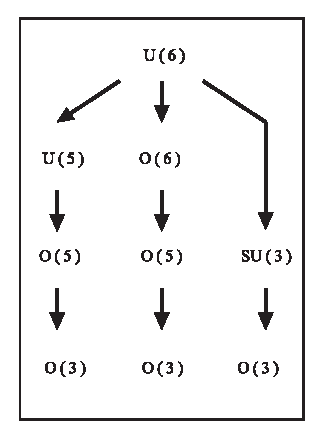
\includegraphics[height=4cm]{figure.eps}
%
% If not, use
%\picplace{5cm}{2cm} % Give the correct figure height and width in cm
%
\caption{Please write your figure caption here}
\label{fig:1}       % Give a unique label
\end{figure}
%
% For built-in environments use
%
\begin{theorem}
Theorem text goes here.
\end{theorem}
%
% or
%
\begin{lemma}
Lemma text goes here.
\end{lemma}
%
%
% Problems or Exercises should be sorted chapterwise
\section*{Problems}
\addcontentsline{toc}{section}{Problems}
%
% Use the following environment.
% Don't forget to label each problem;
% the label is needed for the solutions' environment
\begin{prob}
\label{prob1}
The problem\footnote{Footnote} is described here. The
problem is described here. The problem is described here.
\end{prob}

\begin{prob}
\label{prob2}
\textbf{Problem Heading}\\
(a) The first part of the problem is described here.\\
(b) The second part of the problem is described here.
\end{prob}



%

%!TEX root = book.tex

\chapter{Giới thiệu}
\label{cha:introduce}



Những năm gần đây, AI - Artificial Intelligence (Trí Tuệ Nhân Tạo), và cụ thể hơn là Machine Learning (Học Máy hoặc Máy Học - {\it Với những từ chuyên ngành, tôi sẽ dùng song song cả tiếng Anh và tiếng Việt, tuy nhiên sẽ ưu tiên tiếng Anh vì thuận tiện hơn trong việc tra cứu}) nổi lên như một bằng chứng của cuộc cách mạng công nghiệp lần thứ tư (1 - động cơ hơi nước, 2 - năng lượng điện, 3 - công nghệ thông tin). Trí Tuệ Nhân Tạo đang len lỏi vào mọi lĩnh vực trong đời sống mà có thể chúng ta không nhận ra. Xe tự hành của Google và Tesla, hệ thống tự tag khuôn mặt trong ảnh của Facebook, trợ lý ảo Siri của Apple, hệ thống gợi ý sản phẩm của Amazon, hệ thống gợi ý phim của Netflix, máy chơi cờ vây AlphaGo của Google DeepMind, ..., chỉ là một vài trong vô vàn những ứng dụng của AI/Machine Learning. (Xem thêm \href{{https://www.facebook.com/zuck/posts/10103351073024591}}{Jarvis - trợ lý thông minh cho căn nhà của Mark Zuckerberg}.)

% \url{https://www.facebook.com/zuck/posts/10103351073024591}


Machine Learning là một tập con của AI. Theo định nghĩa của Wikipedia, {\it Machine learning is the subfield of computer science that "gives computers the ability to learn without being explicitly programmed"}. Nói đơn giản, Machine Learning là một lĩnh vực nhỏ của Khoa Học Máy Tính, nó có khả năng tự học hỏi dựa trên dữ liệu đưa vào mà không cần phải được lập trình cụ thể. Bạn Nguyễn Xuân Khánh tại đại học Maryland đang viết một cuốn sách về Machine Learning bằng tiếng Việt khá thú vị, các bạn có thể tham khảo bài \href{https://ml-book-vn.khanhxnguyen.com/intro.html}{Machine Learning là gì?}.

Những năm gần đây, {khi mà khả năng tính toán} của các máy tính được nâng lên một tầm cao mới và lượng dữ liệu khổng lồ được thu thập bởi các hãng công nghệ lớn, Machine Learning đã tiến thêm một bước tiến dài và một lĩnh vực mới được ra đời gọi là Deep Learning (Học Sâu). Deep Learning đã giúp máy tính thực thi những việc tưởng chừng như không thể vào 10 năm trước: phân loại cả ngàn vật thể khác nhau trong các bức ảnh, tự tạo chú thích cho ảnh, bắt chước giọng nói và chữ viết của con người, giao tiếp với con người, hay thậm chí cả sáng tác văn hay âm nhạc (Xem thêm \href{{http://machinelearningmastery.com/inspirational-applications-deep-learning/}}{8 Inspirational Applications of Deep Learning}).

Mối quan hệ giữa Artificial Intelligence, Machine Learning, và Deep Learning được cho trong Hình \ref{fig:aimldl}.

\begin{figure}
\centering
	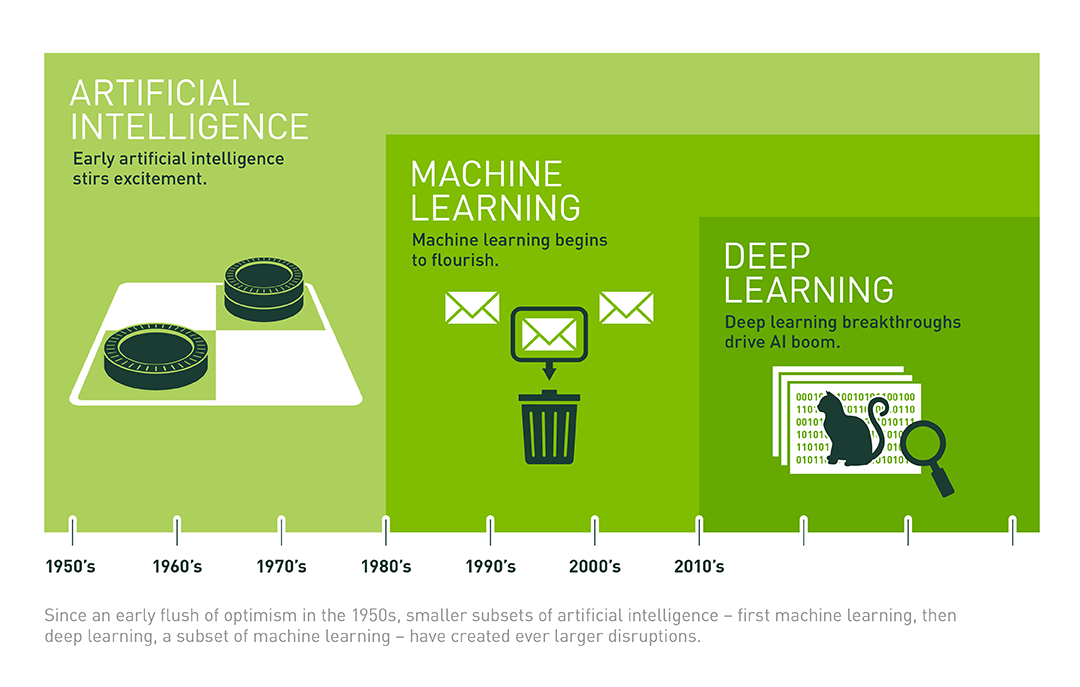
\includegraphics[width = \textwidth]{../introduce/aimldl.png}
	\caption[]{Mối quan hệ giữa AI, Machine Learning và Deep Learning. Nguồn: \href{https://blogs.nvidia.com/blog/2016/07/29/whats-difference-artificial-intelligence-machine-learning-deep-learning-ai/}{What’s the Difference Between Artificial Intelligence, Machine Learning, and Deep Learning?}}
	\label{fig:aimldl}
\end{figure}

% <div class="imgcap">
% <div >
%     <img src="/assets/introduce/aimldl.png" width = "800"></a>
%     <!-- <img src="/assets/rl/mdp.png" height="206"> -->
% </div>
% <div class="thecap">Mối quan hệ giữa AI, Machine Learning và Deep Learning. <br> (Nguồn: <a href="https://blogs.nvidia.com/blog/2016/07/29/whats-difference-artificial-intelligence-machine-learning-deep-learning-ai/">What’s the Difference Between Artificial Intelligence, Machine Learning, and Deep Learning?</a>)</div>
% </div>

\section{Mục đích viết Blog}
Nhu cầu về nhân lực ngành Machine Learning (Deep Learning) đang ngày một cao, kéo theo đó nhu cầu học Machine Learning trên thế giới và ở Việt Nam ngày một lớn. Cá nhân tôi cũng muốn hệ thống lại kiến thức của mình về lĩnh vực này để chuẩn bị cho tương lai (đây là một trong những mục tiêu của tôi trong năm 2017). Tôi sẽ cố gắng đi từ những thuật toán cơ bản nhất của Machine Learning kèm theo các ví dụ và mã nguồn trong mỗi bài viết. Tôi sẽ viết 1-2 tuần 1 bài (việc viết các công thức toán và code trên blog thực sự tốn nhiều thời gian hơn tôi từng nghĩ). Đồng thơi, tôi cũng mong muốn nhận được phản hồi của bạn đọc để qua những thảo luận, tôi và các bạn có thể nắm bắt được các thuật toán này. 

Khi chuẩn bị các bài viết, tôi sẽ giả định rằng bạn đọc có một chút kiến thức về Đại Số Tuyến Tính (Linear Algebra), Xác Suât Thống Kê (Probability and Statistics) và có kinh nghiệm về lập trình Python. Nếu bạn chưa có nhiều kinh nghiệm về các lĩnh vực này, đừng quá lo lắng vì mỗi bài sẽ chỉ sử dụng một vài kỹ thuật cơ bản. Hãy để lại câu hỏi của bạn ở phần Comment bên dưới mỗi bài, tôi sẽ thảo luận thêm với các bạn.

Trong bài tiếp theo của blog này, tôi sẽ giới thiệu về các nhóm thuật toán Machine learning cơ bản. Mời các bạn theo dõi. 

\section{Tham khảo thêm}
\subsection{Các khóa học}
\subsubsection{Tiếng Anh}
\begin{enumerate}
	\item \href{https://www.coursera.org/learn/machine-learning}{Machine Learning với thầy Andrew Ng trên Coursera} ({\it Khóa học nổi tiếng nhất về Machine Learning })

	\item \href{https://www.udacity.com/course/deep-learning--ud730}{Deep Learning by Google trên Udacity} ({\it Khóa học nâng cao hơn về Deep Learning với Tensorflow})


	\item \href{http://machinelearningmastery.com/}{Machine Learning mastery} ({\it Các thuật toán Machine Learning cơ bản})
\end{enumerate}

\subsubsection{Tiếng Việt}
{\bf Lưu ý}: {\it Các khóa học này tôi chưa từng tham gia, chỉ đưa ra để các bạn tham khảo.}
\begin{enumerate}
	\item \href{http://tuanvannguyen.blogspot.com/2016/12/cap-nhat-khoa-hoc-ve-machine-learning.html}{Machine Learning 1/2017}


	\item \href{https://techmaster.vn/khoa-hoc/25511/machine-learning-co-ban}{Nhập môn Machine Learning, Tech Master- Cao Thanh Hà {\it POSTECH}}() 

\end{enumerate}

\subsection{Các trang Machine Learning tiếng Việt khác}
\begin{enumerate}
	\item \href{http://viet.jnlp.org/kien-thuc-co-ban-ve-xu-ly-ngon-ngu-tu-nhien/machine-learning-trong-nlp}{Machine Learning trong Xử Lý Ngôn Ngữ Tự Nhiên - Nhóm Đông Du {\it Nhật Bản}}

	\item \href{https://ongxuanhong.wordpress.com/}{Machine Learning cho người mới bắt đầu - Ông Xuân Hồng {\it JAIST}}. 

	
	 \item \href{https://ml-book-vn.khanhxnguyen.com/}{Machine Learning book for Vietnamese - Nguyễn Xuân Khánh \textit{University of Maryland}}
\end{enumerate}
% 3. [Machine Learning trong Xử Lý Ngôn Ngữ Tự Nhiên - Nhóm Đông Du _Nhật Bản_](http://viet.jnlp.org/kien-thuc-co-ban-ve-xu-ly-ngon-ngu-tu-nhien/machine-learning-trong-nlp)
% 4. [Machine Learning cho người mới bắt đầu - Ông Xuân Hồng _JAIST_](https://ongxuanhong.wordpress.com/). 
% 5. [Machine Learning book for Vietnamese - Nguyễn Xuân Khánh _University of Maryland_](https://ml-book-vn.khanhxnguyen.com/)
%!TEX root = ML_book.tex
\chapter{Phân nhóm các thuật toán Machine Learning}

Có hai cách phổ biến phân nhóm các thuật toán Machine learning. Một là dựa trên phương thức học (learning style), hai là dựa trên chức năng (function) (của mỗi thuật toán).

%!TEX root = book.tex
\chapter{Linear Regression }

 
Trong bài này, tôi sẽ giới thiệu một trong những thuật toán cơ bản nhất (và đơn giản nhất) của Machine Learning. Đây là một thuật toán \textit{Supervised learning} có tên \textbf{Linear Regression} (Hồi Quy Tuyến Tính). Bài toán này đôi khi được gọi là \textit{Linear Fitting} (trong thống kê) hoặc \textit{Linear Least Square}. 

\section{Giới thiệu}
 
Quay lại \href{http://machinelearningcoban.com/2016/12/27/categories/#regression-hoi-quy}{ví dụ đơn giản được nêu trong bài trước}: một căn nhà rộng $x_1 ~ \text{m}^2$, có $x_2$ phòng ngủ và cách trung tâm thành phố $x_3~ \text{km}$ có giá là bao nhiêu. Giả sử chúng ta đã có số liệu thống kê từ 1000 căn nhà trong thành phố đó, liệu rằng khi có một căn nhà mới với các thông số về diện tích, số phòng ngủ và khoảng cách tới trung tâm, chúng ta có thể dự đoán được giá của căn nhà đó không? Nếu có thì hàm dự đoán $y = f(\mathbf{x}) $ sẽ có dạng như thế nào. Ở đây $\mathbf{x} = [x_1, x_2, x_3] $ là một vector hàng chứa thông tin \textit{input}, $y$ là một số vô hướng (scalar) biểu diễn \textit{output} (tức giá của căn nhà trong ví dụ này). 
 
\textbf{Lưu ý về ký hiệu toán học:} \textit{trong các bài viết của tôi, các số vô hướng được biểu diễn bởi các chữ cái viết ở dạng không in đậm, có thể viết hoa, ví dụ $x_1, N, y, k$. Các vector được biểu diễn bằng các chữ cái thường in đậm, ví dụ $\mathbf{y}, \mathbf{x}_1 $. Các ma trận được biểu diễn bởi các chữ viết hoa in đậm, ví dụ $\mathbf{X, Y, W} $.} 
 
Một cách đơn giản nhất, chúng ta có thể thấy rằng: i) diện tích nhà càng lớn thì giá nhà càng cao; ii) số lượng phòng ngủ càng lớn thì giá nhà càng cao; iii) càng xa trung tâm thì giá nhà càng giảm. Một hàm số đơn giản nhất có thể mô tả mối quan hệ giữa giá nhà và 3 đại lượng đầu vào là:  
 
 
$$y \approx  f(\mathbf{x}) = \hat{y}$$ 
$$f(\mathbf{x}) =w_1 x_1 + w_2 x_2 + w_3 x_3 + w_0 ~~~~ (1)$$ 
trong đó, $w_1, w_2, w_3, w_0$ là các hằng số,  $w_0$ còn được gọi là bias. Mối quan hệ $y \approx f(\mathbf{x})$ bên trên là một mối quan hệ tuyến tính (linear). Bài toán chúng ta đang làm là một bài toán thuộc loại regression. Bài toán đi tìm các hệ số tối ưu $ \\{w_1, w_2, w_3, w_0 \\}$ chính vì vậy được gọi là bài toán Linear Regression.  
 
\textbf{Chú ý 1:} $y$ là giá trị thực của \textit{outcome} (dựa trên số liệu thống kê chúng ta có trong tập \textit{training data}), trong khi $\hat{y}$ là giá trị mà mô hình Linear Regression dự đoán được. Nhìn chung, $y$ và $\hat{y}$ là hai giá trị khác nhau do có sai số mô hình, tuy nhiên, chúng ta mong muốn rằng sự khác nhau này rất nhỏ. 
 
\textbf{Chú ý 2:} \textit{Linear} hay \textit{tuyến tính} hiểu một cách đơn giản là \textit{thẳng, phẳng}. Trong không gian hai chiều, một hàm số được gọi là \textit{tuyến tính} nếu đồ thị của nó có dạng một \textit{đường thẳng}. Trong không gian ba chiều, một hàm số được goi là \textit{tuyến tính} nếu đồ thị của nó có dạng một \textit{mặt phẳng}. Trong không gian nhiều hơn 3 chiều, khái niệm \textit{mặt phẳng} không còn phù hợp nữa, thay vào đó, một khái niệm khác ra đời được gọi là \textit{siêu mặt phẳng} (\textit{hyperplane}). Các hàm số tuyến tính là các hàm đơn giản nhất, vì chúng thuận tiện trong việc hình dung và tính toán. Chúng ta sẽ được thấy trong các bài viết sau, \textit{tuyến tính} rất quan trọng và hữu ích trong các bài toán Machine Learning. Kinh nghiệm cá nhân tôi cho thấy, trước khi hiểu được các thuật toán \textit{phi tuyến} (non-linear, không phẳng), chúng ta cần nắm vững các kỹ thuật cho các mô hình \textit{tuyến tính}. 
 
 
 
 
 
\section{Phân tích toán học}
 
 
 
 
\subsection{Dạng của Linear Regression }
 
Trong phương trình $(1)$ phía trên, nếu chúng ta đặt $\mathbf{w} = [w_0, w_1, w_2, w_3]^T = $ là vector (cột) hệ số cần phải tối ưu và $\mathbf{\bar{x}} = [1, x_1, x_2, x_3]$ (đọc là \textit{x bar} trong tiếng Anh) là vector (hàng) dữ liệu đầu vào \textit{mở rộng}. Số $1$ ở đầu được thêm vào để phép tính đơn giản hơn và thuận tiện cho việc tính toán. Khi đó, phương trình (1) có thể được viết lại dưới dạng: 
 
$$y \approx \mathbf{\bar{x}}\mathbf{w} = \hat{y}$$ 
 
Chú ý rằng $\mathbf{\bar{x}}$ là một vector hàng. (\href{http://machinelearningcoban.com/math/#luu-y-ve-ky-hieu}{Xem thêm về ký hiệu vector hàng và cột tại đây}) 
 
 
 
\subsection{Sai số dự đoán }
 
Chúng ta mong muốn rằng sự sai khác $e$ giữa giá trị thực $y$ và giá trị dự đoán $\hat{y}$ (đọc là \textit{y hat} trong tiếng Anh) là nhỏ nhất. Nói cách khác, chúng ta muốn giá trị sau đây càng nhỏ càng tốt:  
 
$$ 
\frac{1}{2}e^2 = \frac{1}{2}(y - \hat{y})^2 = \frac{1}{2}(y - \mathbf{\bar{x}}\mathbf{w})^2 
$$ 
 
trong đó hệ số $\frac{1}{2} $ (\textit{lại}) là để thuận tiện cho việc tính toán (khi tính đạo hàm thì số $\frac{1}{2} $ sẽ bị triệt tiêu). Chúng ta cần $e^2$ vì $e = y - \hat{y} $ có thể là một số âm, việc nói $e$ nhỏ nhất sẽ không đúng vì khi $e = - \infty$ là rất nhỏ nhưng sự sai lệch là rất lớn. Bạn đọc có thể tự đặt câu hỏi: \textbf{tại sao không dùng trị tuyệt đối $ \|e\| $ mà lại dùng bình phương $e^2$ ở đây?} Câu trả lời sẽ có ở phần sau.  
 
 
 
 
 
 
\subsection{Hàm mất mát}
 
Điều tương tự xảy ra với tất cả các cặp \textit{(input, outcome)} $ (\mathbf{x}_i, y_i), i = 1, 2, \dots, N $, với $N$ là số lượng dữ liệu quan sát được. Điều chúng ta muốn, tổng sai số là nhỏ nhất, tương đương với việc tìm $ \mathbf{w} $ để hàm số sau đạt giá trị nhỏ nhất: 
 
$$ \mathcal{L}(\mathbf{w}) = \frac{1}{2}\sum_{i=1}^N (y_i - \mathbf{\bar{x}_i}\mathbf{w})^2 ~~~~~(2) $$  
 
Hàm số $\mathcal{L}(\mathbf{w}) $ được gọi là \textbf{hàm mất mát} (loss function) của bài toán Linear Regression. Chúng ta luôn mong muốn rằng sự mất mát (sai số) là nhỏ nhất, điều đó đồng nghĩa với việc  tìm vector hệ số $ \mathbf{w} $  sao cho  
giá trị của hàm mất mát này càng nhỏ càng tốt. Giá trị của $\mathbf{w}$ làm cho hàm mất mát đạt giá trị nhỏ nhất được gọi là \textit{điểm tối ưu} (optimal point), ký hiệu: 
 
$$ \mathbf{w}^* = \arg\min_{\mathbf{w}} \mathcal{L}(\mathbf{w})  $$  
 
Trước khi đi tìm lời giải, chúng ta đơn giản hóa phép toán trong phương trình hàm mất mát $(2)$. Đặt $\mathbf{y} = [y_1; y_2; \dots; y_N]$ là một vector cột chứa tất cả các \textit{output} của \textit{training data}; $ \mathbf{\bar{X}} = [\mathbf{\bar{x}}_1; \mathbf{\bar{x}}_2; \dots; \mathbf{\bar{x}}_N ] $ là ma trận dữ liệu đầu vào (mở rộng) mà mỗi hàng của nó là một điểm dữ liệu. Khi đó hàm số mất mát $\mathcal{L}(\mathbf{w})$ được viết dưới dạng ma trận đơn giản hơn: 
 
$$ 
\mathcal{L}(\mathbf{w})  
= \frac{1}{2}\sum_{i=1}^N (y_i - \mathbf{\bar{x}}_i\mathbf{w})^2 $$ 
$$ 
= \frac{1}{2} \|\mathbf{y} - \mathbf{\bar{X}}\mathbf{w} \|_2^2  
~~~(3) 
$$ 
 
với $ \| \mathbf{z} \|_2 $ là Euclidean norm (chuẩn Euclid, hay khoảng cách Euclid), nói cách khác $ \| \mathbf{z} \|_2^2 $ là tổng của bình phương mỗi phần tử của vector $\mathbf{z}$. Tới đây, ta đã có một dạng đơn giản của hàm mất mát được viết như phương trình $(3)$. 
 
 
 
 
 
\subsection{Nghiệm cho bài toán Linear Regression}
 
\textbf{Cách phổ biến nhất để tìm nghiệm cho một bài toán tối ưu (chúng ta đã biết từ khi học cấp 3) là giải phương trình đạo hàm (gradient) bằng 0!} Tất nhiên đó là khi việc tính đạo hàm và việc giải phương trình đạo hàm bằng 0 không quá phức tạp. Thật may mắn, với các mô hình tuyến tính, hai việc này là khả thi.  
 
Đạo hàm theo $\mathbf{w} $ của hàm mất mát là:  
$$ 
\frac{\partial{\mathcal{L}(\mathbf{w})}}{\partial{\mathbf{w}}}  
= \mathbf{\bar{X}}^T(\mathbf{\bar{X}}\mathbf{w} - \mathbf{y})  
$$ 
 
Các bạn có thể tham khảo bảng đạo hàm theo vector hoặc ma trận của một hàm số trong \href{https://ccrma.stanford.edu/~dattorro/matrixcalc.pdf}{mục D.2 của tài liệu này}. \textit{Đến đây tôi xin quay lại câu hỏi ở phần Sai số dự đoán phía trên về việc tại sao không dùng trị tuyệt đối mà lại dùng bình phương. Câu trả lời là hàm bình phương có đạo hàm tại mọi nơi, trong khi hàm trị tuyệt đối thì không (đạo hàm không xác định tại 0)}. 
 
Phương trình đạo hàm bằng 0 tương đương với:  
$$ 
\mathbf{\bar{X}}^T\mathbf{\bar{X}}\mathbf{w} = \mathbf{\bar{X}}^T\mathbf{y} \triangleq \mathbf{b}  
~~~ (4) 
$$ 
(ký hiệu $\mathbf{\bar{X}}^T\mathbf{y} \triangleq \mathbf{b} $ nghĩa là \textit{đặt} $\mathbf{\bar{X}}^T\mathbf{y}$ \textit{bằng} $\mathbf{b}$ ). 
 
Nếu ma trận vuông $ \mathbf{A} \triangleq \mathbf{\bar{X}}^T\mathbf{\bar{X}}$ khả nghịch (non-singular hay inversable) thì phương trình $(4)$ có nghiệm duy nhất: $ \mathbf{w} = \mathbf{A}^{-1}\mathbf{b}  $. 
 
Vậy nếu ma trận $\mathbf{A} $ không khả nghịch (có định thức bằng 0) thì sao? Nếu các bạn vẫn nhớ các kiến thức về hệ phương trình tuyến tính, trong trường hợp này thì hoặc phương trinh $ (4) $ vô nghiệm, hoặc làp  
nó 
có vô số nghiệm. Khi đó, chúng ta sử dụng khái niệm \href{https://vi.wikipedia.org/wiki/Giả_nghịch_đảo_Moore–Penrose}{\textit{giả nghịch đảo}} $ \mathbf{A}^{\dagger} $ (đọc là \textit{A dagger} trong tiếng Anh). (\textit{Giả nghịch đảo (pseudo inverse) là trường hợp tổng quát của nghịch đảo khi ma trận không khả nghịch hoặc thậm chí không vuông. Trong khuôn khổ bài viết này, tôi xin phép được lược bỏ phần này, nếu các bạn thực sự quan tâm, tôi sẽ viết một bài khác chỉ nói về giả nghịch đảo. Xem thêm: \href{http://www.sci.utah.edu/~gerig/CS6640-F2012/Materials/pseudoinverse-cis61009sl10.pdf}{Least Squares, Pseudo-Inverses, PCA \& SVD}.}) 
 
Với khái niệm giả nghịch đảo, điểm tối ưu của bài toán Linear Regression có dạng: 
 
 
$$ 
\mathbf{w} = \mathbf{A}^{\dagger}\mathbf{b} = (\mathbf{\bar{X}}^T\mathbf{\bar{X}})^{\dagger} \mathbf{\bar{X}}^T\mathbf{y} 
~~~ (5) 
$$ 
 
 
 
 
\section{Ví dụ trên Python}
 
 
\subsection{Bài toán}
 
Trong phần này, tôi sẽ chọn một ví dụ đơn giản về việc giải bài toán Linear Regression trong Python. Tôi cũng sẽ so sánh nghiệm của bài toán khi giải theo phương trình $(5) $ và nghiệm tìm được khi dùng thư viện \href{http://scikit-learn.org/stable/}{scikit-learn} của Python. (\textit{Đây là thư viện Machine Learning được sử dụng rộng rãi trong Python}). Trong ví dụ này, dữ liệu đầu vào chỉ có 1 giá trị (1 chiều) để thuận tiện cho việc minh hoạ trong mặt phẳng.  
 
Chúng ta có 1 bảng dữ liệu về chiều cao và cân nặng của 15 người như dưới đây: 
 
 
| Chiều cao (cm)     | Cân nặng (km)     | Chiều cao (cm)     | Cân nặng (kg)     | 
| :----------------: | :---------------: | :----------------: | :---------------: | 
| 147                | 49                | 168                | 60                | 
| 150                | 50                | 170                | 72                | 
| 153                | 51                | 173                | 63                | 
| 155                | 52                | 175                | 64                | 
| 158                | 54                | 178                | 66                | 
| 160                | 56                | 180                | 67                | 
| 163                | 58                | 183                | 68                | 
| 165                | 59                |                    |                   | 
 
 
Bài toán đặt ra là: liệu có thể dự đoán cân nặng của một người dựa vào chiều cao của họ không? (\textit{Trên thực tế, tất nhiên là không, vì cân nặng còn phụ thuộc vào nhiều yếu tố khác nữa, thể tích chẳng hạn}). Vì blog này nói về các thuật toán Machine Learning đơn giản nên tôi sẽ giả sử rằng chúng ta có thể dự đoán được. 
 
Chúng ta có thể thấy là cân nặng sẽ tỉ lệ thuận với chiều cao (càng cao càng nặng), nên có thể sử dụng Linear Regression model cho việc dự đoán này. Để kiểm tra độ chính xác của model tìm được, chúng ta sẽ giữ lại cột 155 và 160 cm để kiểm thử, các cột còn lại được sử dụng để huấn luyện (train) model. 
 
 
\subsection{Hiển thị dữ liệu trên đồ thị}
Trước tiên, chúng ta cần có hai thư viện \href{http://www.numpy.org/}{numpy} cho đại số tuyến tính và \href{http://matplotlib.org/}{matplotlib} cho việc vẽ hình.  
 
 
\begin{lstlisting}[language=Python]
# To support both python 2 and python 3 
from __future__ import division, print_function, unicode_literals 
import numpy as np  
import matplotlib.pyplot as plt 
\end{lstlisting}
 
Tiếp theo, chúng ta khai báo và biểu diễn dữ liệu trên một đồ thị. 
 
 
\begin{lstlisting}[language=Python]
# height (cm) 
X = np.array([[147, 150, 153, 158, 163, 165, 168, 170, 173, 175, 178, 180, 183]]).T 
# weight (kg) 
y = np.array([[ 49, 50, 51,  54, 58, 59, 60, 62, 63, 64, 66, 67, 68]]).T 
# Visualize data  
plt.plot(X, y, 'ro') 
plt.axis([140, 190, 45, 75]) 
plt.xlabel('Height (cm)') 
plt.ylabel('Weight (kg)') 
plt.show() 
\end{lstlisting}
 
 
% <div class="imgcap"> 
% <img src ="/assets/LR/output_3_0.png" align = "center"> 
% </div> 
 
 \begin{figure}
 	\centering	
 	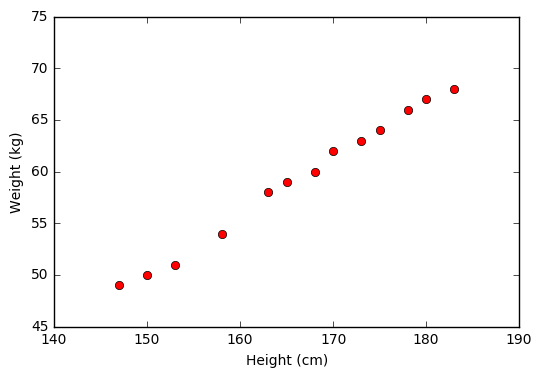
\includegraphics[width = \textwidth]{../LR/output_3_0.png}
 \end{figure}
 
Từ đồ thị này ta thấy rằng dữ liệu được sắp xếp gần như theo 1 đường thẳng, vậy mô hình Linear Regression nhiều khả năng sẽ cho kết quả tốt: 
 
(cân nặng) = \pythoninline{w\_1}*(chiều cao) + \pythoninline{w\_0} 
 
 
\subsection{Nghiệm theo công thức}
 
Tiếp theo, chúng ta sẽ tính toán các hệ số \pythoninline{w_1} và \pythoninline{w_0} dựa vào công thức $(5)$. Chú ý: giả nghịch đảo của một ma trận \pythoninline{A} trong Python sẽ được tính bằng \pythoninline{numpy.linalg.pinv(A)}, \pythoninline{pinv} là từ viết tắt của \textit{pseudo inverse}. 
 
\begin{lstlisting}[language=Python]
# Building Xbar  
one = np.ones((X.shape[0], 1)) 
Xbar = np.concatenate((one, X), axis = 1) 
 
# Calculating weights of the fitting line  
A = np.dot(Xbar.T, Xbar) 
b = np.dot(Xbar.T, y) 
w = np.dot(np.linalg.pinv(A), b) 
print('w = ', w) 
# Preparing the fitting line  
w_0 = w[0][0] 
w_1 = w[1][0] 
x0 = np.linspace(145, 185, 2) 
y0 = w_0 + w_1*x0 
 
# Drawing the fitting line  
plt.plot(X.T, y.T, 'ro')     # data  
plt.plot(x0, y0)               # the fitting line 
plt.axis([140, 190, 45, 75]) 
plt.xlabel('Height (cm)') 
plt.ylabel('Weight (kg)') 
plt.show() 
 
\end{lstlisting}
 
\begin{lstlisting}[language=Python]
w =  [[-33.73541021] 
 [  0.55920496]] 
\end{lstlisting}
 
 


\begin{figure}
	\centering
	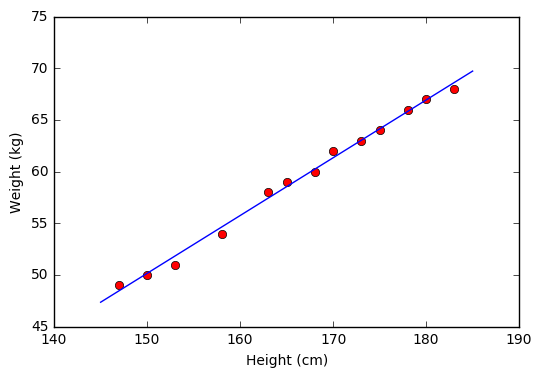
\includegraphics[width = \textwidth]{../LR/output_5_1.png}
\end{figure}
 
Từ đồ thị bên trên ta thấy rằng các điểm dữ liệu màu đỏ nằm khá gần đường thẳng dự đoán màu xanh. Vậy mô hình Linear Regression hoạt động tốt với tập dữ liệu \textit{training}. Bây giờ, chúng ta sử dụng mô hình này để dự đoán cân nặng của hai người có chiều cao 155 và 160 cm mà chúng ta đã không dùng khi tính toán nghiệm. 
 
 
\begin{lstlisting}[language=Python]
y1 = w_1*155 + w_0 
y2 = w_1*160 + w_0 
 
print( 'Predict weight of person with height 155 cm: %.2f (kg), real number: 52 (kg)'  %(y1) ) 
print( 'Predict weight of person with height 160 cm: %.2f (kg), real number: 56 (kg)'  %(y2) ) 
\end{lstlisting}
 
    Predict weight of person with height 155 cm: 52.94 (kg), real number: 52 (kg) 
    Predict weight of person with height 160 cm: 55.74 (kg), real number: 56 (kg) 
 
 
 
Chúng ta thấy rằng kết quả dự đoán khá gần với số liệu thực tế. 
 
 
\subsection{Nghiệm theo thư viện scikit-learn}
 
Tiếp theo, chúng ta sẽ sử dụng thư viện scikit-learn của Python để tìm nghiệm.  
 
 
\begin{lstlisting}[language=Python]
from sklearn import datasets, linear_model 
 
# fit the model by Linear Regression 
regr = linear_model.LinearRegression(fit_intercept=False) # fit_intercept = False for calculating the bias 
regr.fit(Xbar, y) 
 
# Compare two results 
print( 'Solution found by scikit-learn  : ', regr.coef_ ) 
print( 'Solution found by (5): ', w.T) 
\end{lstlisting}
 
\begin{lstlisting}[language=Python]
    Solution found by scikit-learn  :  [[  -33.73541021 0.55920496]] 
    Solution found by (5):  [[  -33.73541021 0.55920496 ]] 
\end{lstlisting}
 
Chúng ta thấy rằng hai kết quả thu được như nhau! (\textit{Nghĩa là tôi đã không mắc lỗi nào trong cách tìm nghiệm ở phần trên}) 
 
\href{https://github.com/tiepvupsu/tiepvupsu.github.io/blob/master/assets/LR/LR.ipynb}{Source code Jupyter Notebook cho bài này.} 
 
 
 
\section{Thảo luận}
 
 
\subsection{Các bài toán có thể giải bằng Linear Regression}
Hàm số $y \approx f(\mathbf{x})= \mathbf{w}^T\mathbf{x}$ là một hàm tuyến tính theo cả $ \mathbf{w}$ và $\mathbf{x}$. Trên thực tế, Linear Regression có thể áp dụng cho các mô hình chỉ cần tuyến tính theo $\mathbf{w}$. Ví dụ: 
$$ 
y \approx w_1 x_1 + w_2 x_2 + w_3 x_1^2 +  w_4 \sin(x_2) + w_5 x_1x_2 + w_0 
$$ 
là một hàm tuyến tính theo $\mathbf{w}$ và vì vậy cũng có thể được giải bằng Linear Regression. Với mỗi dữ liệu đầu vào $\mathbf{x}=[x_1; x_2] $, chúng ta tính toán dữ liệu mới $\tilde{\mathbf{x}} = [x_1, x_2, x_1^2, \sin(x_2), x_1x_2]$ (đọc là \textit{x tilde} trong tiếng Anh) rồi áp dụng Linear Regression với dữ liệu mới này.  
 
Xem thêm ví dụ về \href{http://www.varsitytutors.com/hotmath/hotmath_help/topics/quadratic-regression}{Quadratic Regression} (Hồi Quy Bậc Hai). 
% <div class="imgcap"> 
% <div > 
%     <img src ="http://www.varsitytutors.com/assets/vt-hotmath-legacy/hotmath_help/topics/quadratic-regression/f-qr-1-1.gif"  width = "300"></a> 
% </div> 
% <div class="thecap"> Quadratic Regression (Nguồn: <a href = "http://www.varsitytutors.com/hotmath/hotmath_help/topics/quadratic-regression"> Quadratic Regression</a>) <br></div> 
% </div> 
 
 a figre should be here 
 
\subsection{Hạn chế của Linear Regression}
 
Hạn chế đầu tiên của Linear Regression là nó rất \textbf{nhạy cảm với nhiễu} (sensitive to noise). Trong ví dụ về mối quan hệ giữa chiều cao và cân nặng bên trên, nếu có chỉ 
một cặp dữ liệu \textit{nhiễu} (150 cm, 90kg) thì kết quả sẽ sai khác đi rất nhiều. Xem hình dưới đây: 
% <div class="imgcap"> 
% <img src ="/assets/LR/output_13_1.png" align = "center"> 
% </div> 
 
 \begin{figure}
 	\centering
 	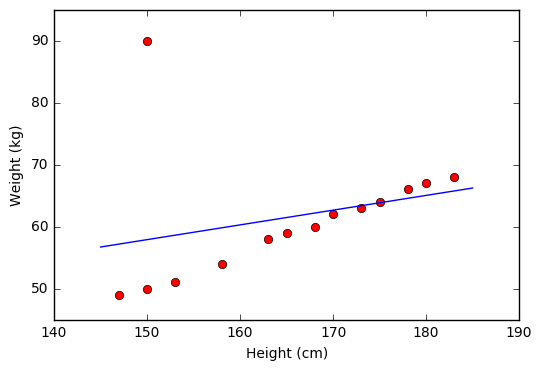
\includegraphics[width = .6\textwidth]{../LR/output_13_1.png}
 \end{figure}
Vì vậy, trước khi thực hiện Linear Regression, các nhiễu (\textit{outlier}) cần 
 phải được loại bỏ. Bước này được gọi là tiền xử lý (pre-processing). 
 
Hạn chế thứ hai của Linear Regression là nó \textbf{không biễu diễn được các mô hình phức tạp}. Mặc dù trong phần trên, chúng ta thấy rằng phương pháp này có thể được áp dụng nếu quan hệ giữa \textit{outcome} và \textit{input} không nhất thiết phải là tuyến tính, nhưng mối quan hệ này vẫn đơn giản nhiều so với các mô hình thực tế. Hơn nữa, chúng ta sẽ tự hỏi: làm thế nào để xác định được các hàm $x_1^2, \sin(x_2), x_1x_2$ như ở trên?! 
 
 
\subsection{Các phương pháp tối ưu}
Linear Regression là một mô hình đơn giản, lời giải cho phương trình đạo hàm bằng 0 cũng khá đơn giản. \textit{Trong hầu hết các trường hợp, chúng ta không thể giải được phương trình đạo hàm bằng 0.} 
 
Nhưng có một điều chúng ta nên nhớ, \textbf{còn tính được đạo hàm là còn có cơ hội}. 
 
 
 
 
\section{Tài liệu tham khảo}
 
1. \href{https://en.wikipedia.org/wiki/Linear_regression}{Linear Regression - Wikipedia} 
2. \href{http://machinelearningmastery.com/simple-linear-regression-tutorial-for-machine-learning/}{Simple Linear Regression Tutorial for Machine Learning} 
3. \href{http://www.sci.utah.edu/~gerig/CS6640-F2012/Materials/pseudoinverse-cis61009sl10.pdf}{Least Squares, Pseudo-Inverses, PCA \& SVD} 

%!TEX root = book.tex
\chapter{K-means Clustering}
\section{Giới thiệu}
\href{http://machinelearningcoban.com/2016/12/28/linearregression/}{Trong bài trước}, chúng ta đã làm quen với thuật toán Linear Regression - là thuật toán đơn giản nhất trong \href{http://machinelearningcoban.com/2016/12/27/categories/#supervised-learning-hoc-co-giam-sat}{Supervised learning}. Bài này tôi sẽ giới thiệu một trong những thuật toán cơ bản nhất trong \href{http://machinelearningcoban.com/2016/12/27/categories/#unsupervised-learning-hoc-khong-giam-sat}{Unsupervised learning} - thuật toán K-means clustering (phân cụm K-means).  
 
  
 
Trong thuật toán K-means clustering, chúng ta không biết nhãn (label) của từng điểm dữ liệu. Mục đích là làm thể nào để phân dữ liệu thành các cụm (cluster) khác nhau sao cho \textit{dữ liệu trong cùng một cụm có tính chất giống nhau}.  
 
\textbf{Ví dụ:} Một công ty muốn tạo ra những chính sách ưu đãi cho những nhóm khách hàng khác nhau dựa trên sự tương tác giữa mỗi khách hàng với công ty đó (số năm là khách hàng; số tiền khách hàng đã chi trả cho công ty; độ tuổi; giới tính; thành phố; nghề nghiệp; ...). Giả sử công ty đó có rất nhiều dữ liệu của rất nhiều khách hàng nhưng chưa có cách nào chia toàn bộ khách hàng đó thành một số nhóm/cụm khác nhau. Nếu một người biết Machine Learning được đặt câu hỏi này, phương pháp đầu tiên anh (chị) ta nghĩ đến sẽ là K-means Clustering. Vì nó là một trong những thuật toán đầu tiên mà anh ấy tìm được trong các cuốn sách, khóa học về Machine Learning. Và tôi cũng chắc rằng anh ấy đã đọc blog <a href = "https://tiepvupsu.github.io">Machine Learning cơ bản</a>. Sau khi đã phân ra được từng nhóm, nhân viên công ty đó có thể lựa chọn ra một vài khách hàng trong mỗi nhóm để quyết định xem mỗi nhóm tương ứng với nhóm khách hàng nào. Phần việc cuối cùng này cần sự can thiệp của con người, nhưng lượng công việc đã được rút gọn đi rất nhiều.  
 
Ý tưởng đơn giản nhất về cluster (cụm) là tập hợp các điểm \textit{ở gần nhau trong một không gian nào đó} (không gian này có thể có rất nhiều chiều trong trường hợp thông tin về một điểm dữ liệu là rất lớn). Hình bên dưới là một ví dụ về 3 cụm dữ liệu (từ giờ rôi sẽ viết gọn là \textit{cluster}).  
 
 
% <div class="imgcap"> 
% <img src ="/assets/kmeans/figure_2.png" width = "500" align = "center"> 
% <div class="thecap"> Bài toán với 3 clusters. <br></div> 
% </div> 
 
Giả sử mỗi cluster có một điểm đại diện (\textit{center}) màu vàng. Và những điểm xung quanh mỗi center thuộc vào cùng nhóm với center đó. Một cách đơn giản nhất, xét một điểm bất kỳ, ta xét xem điểm đó gần với center nào nhất thì nó thuộc về cùng nhóm với center đó. Tới đây, chúng ta có một bài toán thú vị: \textit{Trên một vùng biển hình vuông lớn có ba đảo hình vuông, tam giác, và tròn màu vàng như hình trên. Một điểm trên biển được gọi là thuộc lãnh hải của một đảo nếu nó nằm gần đảo này hơn so với hai đảo kia . Hãy xác định ranh giới lãnh hải của các đảo.} 
 
Hình dưới đây là một hình minh họa cho việc phân chia lãnh hải nếu có 5 đảo khác nhau được biểu diễn bằng các hình tròn màu đen: 
% <div class="imgcap"> 
% <img src ="/assets/kmeans/figure_1.png" width = "500" align = "center"> 
% <div class="thecap"> Phân vùng lãnh hải của mỗi đảo. Các vùng khác nhau có màu sắc khác nhau. <br></div> 
% </div> 
 
Chúng ta thấy rằng đường phân định giữa các lãnh hải là các đường thẳng (chính xác hơn thì chúng là các đường trung trực của các cặp điểm gần nhau). Vì vậy, lãnh hải của một đảo sẽ là một hình đa giác.  
 
Cách phân chia này trong toán học được gọi là \href{https://en.wikipedia.org/wiki/Voronoi_diagram}{Voronoi Diagram}. 
 
Trong không gian ba chiều, lấy ví dụ là các hành tinh, thì (tạm gọi là) \textit{lãnh không} của mỗi hành tinh sẽ là một đa diện. Trong không gian nhiều chiều hơn, chúng ta sẽ có những thứ (mà tôi gọi là) \textit{siêu đa diện} (hyperpolygon). 
 
Quay lại với bài toán phân nhóm và cụ thể là thuật toán K-means clustering, chúng ta cần một chút phân tích toán học trước khi đi tới phần \href{http://machinelearningcoban.com#tom-tat-thuat-toan}{tóm tắt thuật toán} ở phần dưới. Nếu bạn không muốn đọc quá nhiều về toán, bạn có thể bỏ qua phần này. (\textit{Tốt nhất là đừng bỏ qua, bạn sẽ tiếc đấy}). 
 
\section{Phân tích toán học }
 
Mục đích cuối cùng của thuật toán phân nhóm này là: từ dữ liệu đầu vào và số lượng nhóm chúng ta muốn tìm, hãy chỉ ra center của mỗi nhóm và phân các điểm dữ liệu vào các nhóm tương ứng. Giả sử thêm rằng mỗi điểm dữ liệu chỉ thuộc vào đúng một nhóm.  
 
 
\subsection{Một số ký hiệu toán học}
Giả sử có $N$ điểm dữ liệu là $ \mathbf{X} = [\mathbf{x}_1, \mathbf{x}_2, \dots, \mathbf{x}_N] \in \mathbb{R}^{d \times N}$ và $K < N$ là số cluster chúng ta muốn phân chia. Chúng ta cần tìm các center $ \mathbf{m}_1, \mathbf{m}_2, \dots, \mathbf{m}_K \in \mathbb{R}^{d \times 1} $ và label của mỗi điểm dữ liệu. 
 
\textbf{Lưu ý về ký hiệu toán học:} \textit{trong các bài viết của tôi, các số vô hướng được biểu diễn bởi các chữ cái viết ở dạng không in đậm, có thể viết hoa, ví dụ $x_1, N, y, k$. Các vector được biểu diễn bằng các chữ cái thường in đậm, ví dụ $\mathbf{m}, \mathbf{x}_1 $. Các ma trận được biểu diễn bởi các chữ viết hoa in đậm, ví dụ $\mathbf{X, M, Y} $. Lưu ý này đã được nêu ở bài <a href = "/2016/12/28/linearregression/">Linear Regression</a>. Tôi xin được không nhắc lại trong các bài tiếp theo.} 
 
Với mỗi điểm dữ liệu $ \mathbf{x}_i $ đặt $\mathbf{y}_i = [y_{i1}, y_{i1}, \dots, y_{iK}]$ là label vector của nó, trong đó nếu $ \mathbf{x}_i $ được phân vào cluster $k$ thì  $y_{ik} = 1$ và $y_{ij} = 0, \forall j \neq k $. Điều này có nghĩa là có đúng một phần tử của vector $\mathbf{y}_i$ là bằng 1 (tương ứng với cluster của $\mathbf{x}_i $), các phần tử còn lại bằng 0. Ví dụ: nếu một điểm dữ liệu có label vector là $[1,0,0,\dots,0]$ thì nó thuộc vào cluster 1, là $[0,1,0,\dots,0]$ thì nó thuộc vào cluster 2, $\dots$. Cách mã hóa label của dữ liệu như thế này được goi là biểu diễn \href{https://en.wikipedia.org/wiki/One-hot}{\textit{one-hot}}. Chúng ta sẽ thấy cách biểu diễn one-hot này rất phổ biến trong Machine Learning ở các bài tiếp theo.  
 
Ràng buộc của $\mathbf{y}_i $ có thể viết dưới dạng toán học như sau: 
\begin{equation}
 y_{ik} \in \\{0, 1\\},~~~ \sum_{k = 1}^K y_{ik} = 1 ~~~ (1) 
\end{equation}
 
 
\subsection{Hàm mất mát và bài toán tối ưu}
 
Nếu ta coi center $\mathbf{m}_k $  là center (hoặc representative) của mỗi cluster và \textit{ước lượng} tất cả các điểm được phân vào cluster này bởi $\mathbf{m}_k $, thì một điểm dữ liệu $\mathbf{x}_i $ được phân vào cluster $k$ sẽ bị sai số là $ (\mathbf{x}_i - \mathbf{m}_k) $. Chúng ta mong muốn sai số này có trị tuyệt đối nhỏ nhất nên (\href{http://machinelearningcoban.com/2016/12/28/linearregression/#sai-so-du-doan}{giống như trong bài Linear Regression}) ta sẽ tìm cách để đại lượng sau đây đạt giá trị nhỏ nhất:  
\begin{equation}
\|\mathbf{x}_i - \mathbf{m}_k\|_2^2 
\end{equation}
Hơn nữa, vì $\mathbf{x}_i $ được phân vào cluster $k$ nên $y_{ik} = 1, y_{ij} = 0, ~\forall j \neq k $. Khi đó, biểu thức bên trên sẽ được viết lại là: 
\begin{equation}
y_{ik}\|\mathbf{x}_i - \mathbf{m}_k\|_2^2 =  \sum_{j=1}^K y_{ij}\|\mathbf{x}_i - \mathbf{m}_j\|_2^2 
\end{equation}
 
(\textit{Hy vọng chỗ này không quá khó hiểu}) 
 
 
 
Sai số cho toàn bộ dữ liệu sẽ là:  
\begin{equation}
\mathcal{L}(\mathbf{Y}, \mathbf{M}) = \sum_{i=1}^N\sum_{j=1}^K y_{ij} \|\mathbf{x}_i - \mathbf{m}_j\|_2^2 
\end{equation}
 
Trong đó $ \mathbf{Y} = [\mathbf{y}_1; \mathbf{y}_2; \dots; \mathbf{y}_N]$, $ \mathbf{M} = [\mathbf{m}_1, \mathbf{m}_2, \dots \mathbf{m}_K] $ lần lượt là các ma trận được tạo bởi label vector của mỗi điểm dữ liệu và center của mỗi cluster. Hàm số mất mát trong bài toán K-means clustering của chúng ta là hàm $\mathcal{L}(\mathbf{Y}, \mathbf{M})$ với ràng buộc như được nêu trong phương trình $(1)$. 
 
Tóm lại, chúng ta cần tối ưu bài toán sau:  
\begin{equation}
\mathbf{Y}, \mathbf{M} = \arg\min_{\mathbf{Y}, \mathbf{M}} \sum_{i=1}^N\sum_{j=1}^K y_{ij} \|\mathbf{x}_i - \mathbf{m}_j\|_2^2~~~~~(2) 
\end{equation}
 \begin{equation}
\text{subject to:} ~~ y_{ij} \in \\{0, 1\\}~~ \forall i, j;~~~ \sum_{j = 1}^K y_{ij} = 1~~\forall i 
\end{equation}
 
(\textit{subject to} nghĩa là \textit{thỏa mãn điều kiện}). 
 
\textbf{Nhắc lại khái niệm $\arg\min$}: Chúng ta biết ký hiệu $\min$ là \textit{giá trị nhỏ nhất của hàm số}, $\arg\min$ chính là \textit{giá trị của biến số để hàm số đó đạt giá trị nhỏ nhất đó}. Nếu $f(x) = x^2 -2x + 1 = (x-1)^2 $ thì giá trị nhỏ nhất của hàm số này bằng 0, đạt được khi $x = 1$. Trong ví dụ này $\min_{x} f(x) = 0$ và $\arg\min_{x} f(x) = 1$. Thêm ví dụ khác, nếu $x_1 = 0, x_2 = 10, x_3 = 5$ thì ta nói $\arg\min_{i} x_i = 1$ vì $1$ là chỉ số để $x_i$ đạt giá trị nhỏ nhất (bằng $0$). Biến số viết bên dưới $\min$ là biến số cúng ta cần tối ưu. Trong các bài toán tối ưu, ta thường quan tâm tới $\arg\min$ hơn là $\min$. 
 
\subsection{Thuật toán tối ưu hàm mất mát}
Bài toán $(2)$ là một bài toán khó tìm \textit{điểm tối ưu} vì nó có thêm các điều kiện ràng buộc. \textit{Bài toán này thuộc loại mix-integer programming (điều kiện biến là số nguyên) - là loại rất khó tìm nghiệm tối ưu toàn cục (global optimal point, tức nghiệm làm cho hàm mất mát đạt giá trị nhỏ nhất có thể).} Tuy nhiên, trong một số trường hợp chúng ta vẫn có thể tìm được phương pháp để tìm được nghiệm gần đúng hoặc điểm cực tiểu. (\textit{Nếu chúng ta vẫn nhớ chương trình toán ôn thi đại học thì điểm cực tiểu chưa chắc đã phải là điểm làm cho hàm số đạt giá trị nhỏ nhất}). 
 
Một cách đơn giản để giải bài toán $(2)$ là xen kẽ giải $\mathbf{Y}$ và $ \mathbf{M}$ khi biến còn lại được cố định. Đây là một thuật toán lặp, cũng là kỹ thuật phổ biến khi giải bài toán tối ưu. Chúng ta sẽ lật lượt giải quyết hai bài toán sau đây: 
 
 
\subsubsection{Cố định $\mathbf{M} $, tìm $\mathbf{Y}$ }
\textbf{Giả sử đã tìm được các centers, hãy tìm các label vector để hàm mất mát đạt giá trị nhỏ nhất.} Điều này tương đương với việc tìm cluster cho mỗi điểm dữ liệu. 
 
Khi các centers là cố định, bài toán tìm label vector cho toàn bộ dữ liệu có thể được chia nhỏ thành bài toán tìm label vector cho từng điểm dữ liệu $\mathbf{x}_i$ như sau: 
\begin{equation}
\mathbf{y}_i = \arg\min_{\mathbf{y}_i} \sum_{j=1}^K y_{ij}\|\mathbf{x}_i - \mathbf{m}_j\|_2^2 ~~~ (3) 
\end{equation}
\begin{equation}
\text{subject to:} ~~ y_{ij} \in \\{0, 1\\}~~ \forall j;~~~ \sum_{j = 1}^K y_{ij} = 1 
\end{equation}
 
Vì chỉ có một phần tử của label vector $\mathbf{y}_i$ bằng $1$ nên bài toán $(3)$ có thể tiếp tục được viết dưới dạng đơn giản hơn:  
\begin{equation}
j = \arg\min_{j} \|\mathbf{x}_i - \mathbf{m}_j\|_2^2 
\end{equation}
 
Vì $\|\mathbf{x}_i - \mathbf{m}_j\|_2^2$ chính là bình phương khoảng cách tính từ điểm $\mathbf{x}_i $ tới center $\mathbf{m}_j $, ta có thể kết luận rằng \textbf{mỗi điểm $\mathbf{x}_i $ thuộc vào cluster có center gần nó nhất}! Từ đó ta có thể dễ dàng suy ra label vector của từng điểm dữ liệu. 
 
 
\subsubsection{Cố định $\mathbf{Y} $, tìm $\mathbf{M}$ }
\textbf{Giả sử đã tìm được cluster cho từng điểm, hãy tìm center mới cho mỗi cluster để hàm mất mát đạt giá trị nhỏ nhất.} 
 
Một khi chúng ta đã xác định được label vector cho từng điểm dữ liệu, bài toán tìm center cho mỗi cluster được rút gọn thành:  
 
\begin{equation}
\mathbf{m}_j = \arg\min_{\mathbf{m}_j} \sum_{i = 1}^{N} y_{ij}\|\mathbf{x}_i - \mathbf{m}_j \|_2^2. 
\end{equation}
 Tới đây, ta có thể tìm nghiệm bằng phương pháp giải đạo hàm bằng 0, vì hàm cần tối ưu là một hàm liên tục và có đạo hàm xác định tại mọi điểm. \textit{Và quan trọng hơn, hàm này là hàm convex (lồi) theo $\mathbf{m}_j $ nên chúng ta sẽ tìm được giá trị nhỏ nhất và điểm tối ưu tương ứng. Sau này nếu có dịp, tôi sẽ nói thêm về tối ưu lồi (convex optimization) - một mảng cực kỳ quan trọng trong toán tối ưu}. 
 
 Đặt $l(\mathbf{m}_j)$ là hàm bên trong dấu $\arg\min$, ta có đạo hàm: 
\begin{equation}
\frac{\partial l(\mathbf{m}_j)}{\partial \mathbf{m}_j} = 2\sum_{i=1}^N y_{ij}(\mathbf{m}_j - \mathbf{x}_i)  
\end{equation}
 
Giải phương trình đạo hàm bằng 0 ta có:  
\begin{equation}
\mathbf{m}_j \sum_{i=1}^N y_{ij} = \sum_{i=1}^N y_{ij} \mathbf{x}_i  
\end{equation}
\begin{equation}
\Rightarrow \mathbf{m}_j = \frac{ \sum_{i=1}^N y_{ij} \mathbf{x}_i}{\sum_{i=1}^N y_{ij}} 
\end{equation}
 
Nếu để ý một chút, chúng ta sẽ thấy rằng mẫu số chính là phép đếm \textit{số lượng các điểm dữ liệu} trong cluster $j$ (\textit{Bạn có nhận ra không?}). Còn tử số chính là \textit{tổng các điểm dữ liệu} trong cluster $j$. (\textit{Nếu bạn đọc vẫn nhớ điều kiện ràng buộc của các} $y_{ij} $ \textit{thì sẽ có thể nhanh chóng nhìn ra điều này}). 
 
Hay nói một cách đơn giản hơn nhiều: $\mathbf{m}_j$ \textbf{là trung bình cộng của các điểm trong cluster} $j$. 
 
Tên gọi \textit{K-means clustering} cũng xuất phát từ đây. 
 
\subsection{Tóm tắt thuật toán}
Tới đây tôi xin được tóm tắt lại thuật toán (\textit{đặc biệt quan trọng với các bạn bỏ qua phần toán học bên trên}) như sau: 
 
\textbf{Đầu vào:} Dữ liệu $\mathbf{X}$ và số lượng cluster cần tìm $K$. 
 
\textbf{Đầu ra:} Các center $\mathbf{M}$ và label vector cho từng điểm dữ liệu $\mathbf{Y}$. 
 
1. Chọn $K$ điểm bất kỳ làm các center ban đầu. 
2. Phân mỗi điểm dữ liệu vào cluster có center gần nó nhất.  
3. Nếu việc gán dữ liệu vào từng cluster ở bước 2 không thay đổi so với vòng lặp trước nó thì ta dừng thuật toán.  
4. Cập nhật center cho từng cluster bằng cách lấy trung bình cộng của tất các các điểm dữ liệu đã được gán vào cluster đó sau bước 2. 
5. Quay lại bước 2. 
 
Chúng ta có thể đảm bảo rằng thuật toán sẽ dừng lại sau một số hữu hạn vòng lặp. Thật vậy, vì hàm mất mát là một số dương và sau mỗi bước 2 hoặc 3, giá trị của hàm mất mát bị giảm đi. Theo kiến thức về dãy số trong chương trình cấp 3: \textit{nếu một dãy số giảm và bị chặn dưới thì nó hội tụ!} Hơn nữa, số lượng cách phân nhóm cho toàn bộ dữ liệu là hữu hạn nên đến một lúc nào đó, hàm mất mát sẽ không thể thay đổi, và chúng ta có thể dừng thuật toán tại đây. 
 
Chúng ta sẽ có một vài \href{http://machinelearningcoban.com#-thao-luan}{thảo luận} về thuật toán này, về những hạn chế và một số phương pháp khắc phục. Nhưng trước hết, hãy xem nó thể hiện như thế nào trong một ví dụ cụ thể dưới đây. 
 
 
\section{Ví dụ trên Python}
 
 
\subsection{Giới thiệu bài toán}
 
Để kiểm tra mức độ hiểu quả của một thuật toán, chúng ta sẽ làm một ví dụ đơn giản (thường được gọi là \textit{toy example}). Trước hết, chúng ta chọn center cho từng cluster và tạo dữ liệu cho từng cluster bằng cách lấy mẫu theo phân phối chuẩn có kỳ vọng là center của cluster đó và ma trận hiệp phương sai (covariance matrix) là ma trận đơn vị.  
 
Trước tiên, chúng ta cần khai báo các thư viện cần dùng. Chúng ta cần \pythoninline{numpy} và \pythoninline{matplotlib} như trong bài \href{http://machinelearningcoban.com/2016/12/28/linearregression/}{Linear Regression} cho việc tính toán ma trận và hiển thị dữ liệu. Chúng ta cũng cần thêm thư viện \pythoninline{scipy.spatial.distance} để tính khoảng cách giữa các cặp điểm trong hai tập hợp một cách hiệu quả. 
 
 
\begin{lstlisting}[language=Python]
import numpy as np  
import matplotlib.pyplot as plt 
from scipy.spatial.distance import cdist 
np.random.seed(11) 
\end{lstlisting}
 
Tiếp theo, ta tạo dữ liệu bằng cách lấy các điểm theo phân phối chuẩn có kỳ vọng tại các điểm có tọa độ \pythoninline{(2, 2), (8, 3)} và \pythoninline{(3, 6)}, ma trận hiệp phương sai giống nhau và là ma trận đơn vị. Mỗi cluster có 500 điểm. (\textit{Chú ý rằng mỗi điểm dữ liệu là một hàng của ma trận dữ liệu.} 
 
 
\begin{lstlisting}[language=Python]
means = [[2, 2], [8, 3], [3, 6]] 
cov = [[1, 0], [0, 1]] 
N = 500 
X0 = np.random.multivariate_normal(means[0], cov, N) 
X1 = np.random.multivariate_normal(means[1], cov, N) 
X2 = np.random.multivariate_normal(means[2], cov, N) 
 
X = np.concatenate((X0, X1, X2), axis = 0) 
K = 3 
 
original_label = np.asarray([0]*N + [1]*N + [2]*N).T 
\end{lstlisting}
 
 
\subsection{Hiển thị dữ liệu trên đồ thị}
 
Chúng ta cần một hàm \pythoninline{kmeans_display} để hiển thị dữ liệu. Sau đó hiển thị dữ liệu theo nhãn ban đầu. 
 
 
\begin{lstlisting}[language=Python]
def kmeans_display(X, label): 
    K = np.amax(label) + 1 
    X0 = X[label == 0, :] 
    X1 = X[label == 1, :] 
    X2 = X[label == 2, :] 
     
    plt.plot(X0[:, 0], X0[:, 1], 'b^', markersize = 4, alpha = .8) 
    plt.plot(X1[:, 0], X1[:, 1], 'go', markersize = 4, alpha = .8) 
    plt.plot(X2[:, 0], X2[:, 1], 'rs', markersize = 4, alpha = .8) 
 
    plt.axis('equal') 
    plt.plot() 
    plt.show() 
     
kmeans_display(X, original_label) 
\end{lstlisting}
 
 
% <div class="imgcap"> 
% <img src ="/assets/kmeans/output_5_0.png" align = "center"> 
% </div> 
Trong đồ thị trên, mỗi cluster tương ứng với một màu. Có thể nhận thấy rằng có một vài điểm màu đỏ bị lẫn sang phần cluster màu xanh. 
 
\subsection{Các hàm số cần thiết cho K-means clustering }
Viết các hàm: 
 
1. \pythoninline{kmeans_init_centers} để khởi tạo các centers ban đầu. 
2. \pythoninline{kmeans_asign_labels} để gán nhán mới cho các điểm khi biết các centers. 
3. \pythoninline{kmeans_update_centers} để cập nhật các centers mới dữa trên dữ liệu vừa được gán nhãn. 
4. \pythoninline{has_converged} để kiểm tra điều kiện dừng của thuật toán. 
 
 
\begin{lstlisting}[language=Python]
def kmeans_init_centers(X, k): 
    # randomly pick k rows of X as initial centers 
    return X[np.random.choice(X.shape[0], k, replace=False)] 
 
def kmeans_assign_labels(X, centers): 
    # calculate pairwise distances btw data and centers 
    D = cdist(X, centers) 
    # return index of the closest center 
    return np.argmin(D, axis = 1) 
 
def kmeans_update_centers(X, labels, K): 
    centers = np.zeros((K, X.shape[1])) 
    for k in range(K): 
        # collect all points assigned to the k-th cluster  
        Xk = X[labels == k, :] 
        # take average 
        centers[k,:] = np.mean(Xk, axis = 0) 
    return centers 
 
def has_converged(centers, new_centers): 
    # return True if two sets of centers are the same 
    return (set([tuple(a) for a in centers]) ==  
        set([tuple(a) for a in new_centers])) 
\end{lstlisting}
 
Phần chính của K-means clustering: 
 
 
\begin{lstlisting}[language=Python]
def kmeans(X, K): 
    centers = [kmeans_init_centers(X, K)] 
    labels = [] 
    it = 0  
    while True: 
        labels.append(kmeans_assign_labels(X, centers[-1])) 
        new_centers = kmeans_update_centers(X, labels[-1], K) 
        if has_converged(centers[-1], new_centers): 
            break 
        centers.append(new_centers) 
        it += 1 
    return (centers, labels, it) 
\end{lstlisting}
 
Áp dụng thuật toán vừa viết vào dữ liệu ban đầu, hiển thị kết quả cuối cùng.  
 
 
\begin{lstlisting}[language=Python]
(centers, labels, it) = kmeans(X, K) 
print 'Centers found by our algorithm:' 
print centers[-1] 
 
kmeans_display(X, labels[-1]) 
\end{lstlisting}
 
    Centers found by our algorithm: 
    [[ 1.97563391  2.01568065] 
     [ 8.03643517  3.02468432] 
     [ 2.99084705  6.04196062]] 
 
% <div class="imgcap"> 
% <img src ="/assets/kmeans/output_11_1.png" align = "center"> 
% </div> 
 
 
 
Từ kết quả này chúng ta thấy rằng thuật toán K-means clustering làm việc khá thành công, các centers tìm được khá gần với kỳ vọng ban đầu. Các điểm thuộc cùng một cluster hầu như được phân vào cùng một cluster (trừ một số diểm màu đỏ ban đầu đã bị phân nhầm vào cluster màu xanh da trời, nhưng tỉ lệ là nhỏ và có thể chấp nhận được). 
 
Dưới đây là hình ảnh động minh họa thuật toán qua từng vòng lặp, chúng ta thấy rằng thuật toán trên hội tụ rất nhanh, chỉ cần 6 vòng lặp để có được kết quả cuối cùng: 
<div class="imgcap"> 
<img src ="/assets/kmeans/kmeans11.gif" align = "center"> 
</div> 
 
 
Các bạn có thể xem thêm các trang web minh họa thuật toán K-means cluster tại: 
\begin{enumerate}
	\item \href{https://www.naftaliharris.com/blog/visualizing-k-means-clustering/}{Visualizing K-Means Clustering}

	\item \href{http://stanford.edu/class/ee103/visualizations/kmeans/kmeans.html}{Visualizing K-Means Clustering - Standford}
 
\end{enumerate}
 
\subsection{Kết quả tìm được bằng thư viện scikit-learn}
 
Để kiểm tra thêm, chúng ta hãy so sánh kết quả trên với kết quả thu được bằng cách sử dụng thư viện \href{http://scikit-learn.org/stable/modules/generated/sklearn.cluster.KMeans.html}{\pythoninline{scikit-learn}}. 
 
\begin{lstlisting}[language=Python]
from sklearn.cluster import KMeans 
kmeans = KMeans(n_clusters=3, random_state=0).fit(X) 
print 'Centers found by scikit-learn:' 
print kmeans.cluster_centers_ 
pred_label = kmeans.predict(X) 
kmeans_display(X, pred_label) 
\end{lstlisting}
 
    Centers found by scikit-learn: 
    [[ 8.0410628   3.02094748] 
     [ 2.99357611  6.03605255] 
     [ 1.97634981  2.01123694]] 
 
 
 
% <div class="imgcap"> 
% <img src ="/assets/kmeans/output_14_1.png" align = "center"> 
% </div> 
 
 
Thật may mắn (\textit{cho tôi}), hai thuật toán cho cùng một đáp số! Với cách thứ nhất, tôi mong muốn các bạn hiểu rõ được thuật toán K-means clustering làm việc như thế nào. Với cách thứ hai, tôi hy vọng các bạn biết áp dụng thư viện sẵn có như thế nào. 
 
 
\section{Thảo luận}
 
\subsection{Hạn chế}
Có một vài hạn chế của thuật toán K-means clustering: 
 
 
\subsubsection{Chúng ta cần biết số lượng cluster cần clustering}
Để ý thấy rằng trong \href{http://machinelearningcoban.com#tom-tat-thuat-toan}{thuật toán nêu trên}, chúng ta cần biết đại lượng $K$ là số lượng clusters. Trong thực tế, nhiều trường hợp chúng ta không xác định được giá trị này. Có một số phương pháp giúp xác định số lượng clusters, tôi sẽ dành thời gian nói về chúng sau nếu có dịp. Bạn đọc có thể tham khảo \href{https://en.wikipedia.org/wiki/Determining_the_number_of_clusters_in_a_data_set}{Elbow method - Determining the number of clusters in a data set}. 
 
 
\subsubsection{Nghiệm cuối cùng phụ thuộc vào các centers được khởi tạo ban đầu}
Tùy vào các center ban đầu mà thuật toán có thể có tốc độ hội tụ rất chậm, ví dụ: 
% <div class="imgcap"> 
% <img src ="/assets/kmeans/kmeans_slowconverge.gif" align = "center"> 
% </div> 
hoặc thậm chí cho chúng ta nghiệm không chính xác (chỉ là local minimum - điểm cực tiểu - mà không phải giá trị nhỏ nhất): 
 
% <div class="imgcap"> 
% <img src ="/assets/kmeans/kmeans_badresult.gif" align = "center"> 
% </div> 
 
Có một vài cách khắc phục đó là: 

\begin{itemize}
	\item Chạy K-means clustering nhiều lần với các center ban đầu khác nhau rồi chọn cách có hàm mất mát cuối cùng đạt giá trị nhỏ nhất.

	\item \href{https://en.wikipedia.org/wiki/K-means%2B%2B#Improved_initialization_algorithm}{K-means++ -Improve initialization algorithm - wiki}. 

	\item Bạn nào muốn tìm hiểu sâu hơn có thể xem bài báo khoa học \href{http://www.sciencedirect.com/science/article/pii/S0167865504000996}{Cluster center initialization algorithm for K-means clustering}. 
 
\end{itemize}
 
\subsubsection{Các cluster cần có só lượng điểm gần bằng nhau}
 
Dưới đây là một ví dụ với 3 cluster với 20, 50, và 1000 điểm. Kết quả cuối cùng không chính xác.  
 
% <div class="imgcap"> 
% <img src ="/assets/kmeans/kmeans_unbalanced.gif" align = "center"> 
% </div> 
 
 
\subsubsection{Các cluster cần có dạng hình tròn }
Tức các cluster tuân theo phân phối chuẩn và ma trận hiệp phương sai là ma trận đường chéo có các điểm trên đường chéo giống nhau. 
 
Dưới đây là 1 ví dụ khi 1 cluster có dạng hình dẹt.  
 
% <div class="imgcap"> 
% <img src ="/assets/kmeans/kmeans_diffcov.gif" align = "center"> 
% </div> 
 
 
\subsubsection{Khi một cluster nằm phía trong 1 cluster khác}
 Đây là ví dụ kinh điển về việc K-means clustering không thể phân cụm dữ liệu. Một cách tự nhiên, chúng ta sẽ phân ra thành 4 cụm: mắt trái, mắt phải, miệng, xunh quanh mặt. Nhưng vì mắt và miệng nằm trong khuôn mặt nên K-means clustering không thực hiện được: 
 
%  <div class="imgcap"> 
% <img src ="/assets/kmeans/smile_face.png" align = "center"> 
% </div> 
 
 
Mặc dù có những hạn chế, K-means clustering vẫn cực kỳ quan trọng trong Machine Learning và là nền tảng cho nhiều thuật toán phức tạp khác sau này. Chúng ta cần bắt đầu từ những thứ đơn giản. \textit{Simple is best!} 
 
 
 
\section{Tài liệu tham khảo}

\begin{enumerate}
	\item \href{http://scikit-learn.org/stable/auto_examples/text/document_clustering.html}{Clustering documents using k-means}

	\item \href{https://en.wikipedia.org/wiki/Voronoi_diagram}{Voronoi Diagram - Wikipedia}

	\item \href{http://www.sciencedirect.com/science/article/pii/S0167865504000996}{Cluster center initialization algorithm for K-means clustering}

	\item \href{https://www.naftaliharris.com/blog/visualizing-k-means-clustering/}{Visualizing K-Means Clustering}

	\item \href{http://stanford.edu/class/ee103/visualizations/kmeans/kmeans.html}{Visualizing K-Means Clustering - Standford}
 
\end{enumerate}
 

%!TEX root = book.tex
\chapter{K-means Clustering: Simple Applications}
Trong bài này, tôi sẽ áp dụng thuật toán \href{http://machinelearningcoban.com/2017/01/01/kmeans/}{K-means clustering} vào ba bài toán xử lý ảnh thực tế hơn: i) Phân nhóm các chữ số viết tay, ii) Tách vật thể (image segmentation) và iii) Nén ảnh/dữ liệu (image compression). Qua đây, tôi cũng muốn độc giả  làm quen với một số kỹ thuật đơn giản trong xử lý hình ảnh - một mảng quan trọng trong Machine Learning. Souce code cho các ví dụ trong trang này có thể được tìm thấy \href{https://github.com/tiepvupsu/tiepvupsu.github.io/blob/master/assets/kmeans/Kmeans2.ipynb}{tại đây}.  

 
\section{Phân nhóm chữ số viết tay }
 
\subsection{Bộ cơ sở dữ liệu MNIST }
\href{http://yann.lecun.com/exdb/mnist/}{Bộ cơ sở dữ liệu MNIST} là bộ cơ sở dữ liệu lớn nhất về chữ số viết tay và được sử dụng trong hầu hết các thuật toán nhận dạng hình ảnh (Image Classification).  
 
MNIST bao gồm hai tập con: tập dữ liệu huấn luyện (training set) có tổng cộng 60k ví dụ khác nhau về chữ số viết tay từ 0 đên 9, tập dữ liệu kiểm tra (test set) có 10k ví dụ khác nhau. Tất cả đều đã được gán nhãn. Hình dưới đây là ví dụ về một số hình ảnh được trích ra từ MNIST. 
 
% <div class="imgcap"> 
%     <img src="http://www.rubylab.io/img/mnist.png" width = "800"> 
% <div class="thecap"><a href = "http://yann.lecun.com/exdb/mnist/">MNIST</a>: bộ cơ sở dữ liệu của chữ số viết tay. <br> (Nguồn: <a href ="http://www.rubylab.io/2015/03/18/simple-neural-network-implenentation-in-ruby/">Simple Neural Network implementation in Ruby)</a></div> 
% </div> 
 
Mỗi bức ảnh là một ảnh đen trắng (có 1 channel), có kích thước 28x28 pixel (tổng cộng 784 pixels). Mỗi pixel mang một giá trị là một số tự nhiên từ 0 đến 255. Các pixel màu đen có giá trị bằng 0, các pixel càng trắng thì có giá trị càng cao (nhưng không quá 255). Dưới đây là một ví dụ về chữ số 7 và giá trị các pixel của nó. (\textit{Vì mục đích hiển thị ma trận pixel ở bên phải, tôi đã resize bức ảnh về 14x14}) 
 
 
% <div class="imgcap"> 
% <img src ="/assets/kmeans/digit_7.png" align = "center"> 
% </div>  
 
 
\subsection{Bài toán phân nhóm giả định}
\textbf{Bài toán: Giả sử rằng chúng ta không biết nhãn của các chữ số này, chúng ta muốn phân nhóm các bức ảnh gần giống nhau về một nhóm.} 
 
Lại thêm một giả sử nữa là chúng ta mới chỉ biết tới thuật toán phân nhóm \href{http://machinelearningcoban.com/2017/01/01/kmeans/}{K-means clustering} gần đây từ blog \href{https://tiepvupsu.github.io/}{Machine Learning cơ bản} (\textit{xin lỗi độc giả vì để các bài học có ý nghĩa hơn, chúng ta đôi khi cần những giả định không được thực tế cho lắm}), chúng ta sẽ giải quyết bài toán này thế nào? 
 
Trước khi áp dụng thuật toán \href{http://machinelearningcoban.com/2017/01/01/kmeans/}{K-means clustering}, chúng ta cần coi mỗi bức ảnh là một điểm dữ liệu. Và vì mỗi điểm dữ liệu là 1 vector (hàng hoặc cột) chứ không phải ma trận như số 7 ở trên, chúng ta phải làm thêm một bước đơn giản trung gian gọi là \textit{vectorization} (vector hóa). Nghĩa là, để có được 1 vector, ta có thể tách các hàng của ma trận pixel ra, sau đó đặt chúng cạnh nhau, và chúng ta được một vector hàng rất dài biểu diễn 1 bức ảnh chữ số.  
 
\textbf{Chú ý}: \textit{Cách làm này chỉ là cách đơn giản nhất để mô tả dữ liệu ảnh bằng 1 vector. Trên thực tế, người ta áp dụng rất nhiều kỹ thuật khác nhau để có thể tạo ra các vector đặc trưng (feature vector) giúp các thuật toán có được kết quả tốt hơn.} 
 
 
\subsection{Làm việc trên Python}
Trước tiên các bạn vào trang chủ của MNIST để \href{http://yann.lecun.com/exdb/mnist/ }{download} bộ cơ sở dữ liệu này. Trong bài này chúng ta chỉ dùng bộ dữ liệu tét với 10k ảnh và không cần label nên các bạn chỉ cần download file \pythoninline{t10k-images-idx3-ubyte.gz} 
 
 
\textbf{Trước tiên chúng ta cần khai báo một số thư viện:} 
 
\pythoninline{numpy} cho các phép toán liên quan đến ma trận. \href{https://pypi.python.org/pypi/python-mnist/}{\pythoninline{mnist}} để đọc dữ liệu từ MNIST. \pythoninline{matplotlib} để hiển thị hình vẽ. \pythoninline{sklearn} chính là \pythoninline{scikit-learn} mà chúng ta đã làm quen trong các bài trước. (\textit{Về việc cài đặt các thư viện này, tôi hy vọng bạn đọc có thể Google thêm đôi chút. Nếu có khó khăn trong việc cài đặt, hãy để lại comment ở dưới bài. Lưu ý, làm việc trên Windows sẽ khó khăn hơn một chút so với Linux}) 
 
\begin{lstlisting}[language=Python]
# %reset 
import numpy as np  
from mnist import MNIST # require `pip install python-mnist` 
import matplotlib.pyplot as plt 
from sklearn.cluster import KMeans 
\end{lstlisting}
 
\textbf{Để hiện thị nhiều bức ảnh các chữ số cùng một lúc, tôi có dùng thêm hàm số \href{https://github.com/tiepvupsu/tiepvupsu.github.io/blob/master/assets/kmeans/display_network.py}{\pythoninline{display_network.py}}}. 
 
\textbf{Thực hiện thuật toán K-means clustering trên toàn bộ 10k chữ số.} 
 
\begin{lstlisting}[language=Python]
from display_network import * 
 
mndata = MNIST('../MNIST/') # path to your MNIST folder  
mndata.load_testing() 
X = mndata.test_images 
 
kmeans = KMeans(n_clusters=K).fit(X) 
pred_label = kmeans.predict(X) 
\end{lstlisting}
 
(\textit{Phần còn lại của source code có thể được tìm thấy \href{https://github.com/tiepvupsu/tiepvupsu.github.io/blob/master/assets/kmeans/Kmeans2.ipynb}{tại đây}}) 
 
Đến đây, sau khi đã tìm được các center và phân nhóm dữ liệu vào từng cluster, tôi muốn hiển thị xem center trông như thế nào và các bức ảnh được phân vào mỗi cluster có giống nhau hay không. Dưới đây là kết quả khi tôi chọn ngẫu nhiên 20 bức ảnh từ mỗi cluster. 
 
% <div class="imgcap"> 
% <img src ="/assets/kmeans/kmeans_random.png" align = "center"> 
% <div class="thecap">Áp dụng K-means clustering vào tập test set của bộ cơ sở dữ liệu MNIST với K = 10 cluster. Cột 1: centers của các cluster. Các cột còn lại: Mỗi hàng là 20 điểm dữ liệu ngẫu nhiên được chọn ra từ mỗi cluster. 
% </div> 
% </div>  
Mỗi hàng tương ứng với một cluster, cột đầu tiên có nền xanh bên trái là centers tìm được của các clusters (màu đỏ hơn là các pixel có giá trị cao hơn). Chúng ta thấy rằng các center đều hoặc là giống với một chữ số nào đó, hoặc là kết hợp của hai/ba chữ số nào đó. Ví dụ: center của nhóm thứ 4 là sự kết hợp của các số 4, 7, 9; của hàng thứ 7 là kết hợp của chữ số 7, 8 và 9.  
 
Tuy nhiên, các bức ảnh lấy ra ngẫu nhiên từ mỗi nhóm trông không thực sự giống nhau. Lý do có thể là những bức ảnh này ở xa các center của mỗi nhóm (mặc dù center đó đã là gần nhất). Như vậy thuật toán K-means clustering làm việc không thực sự tốt trong trường hợp này. (\textit{Thật may là vì thế nên chúng ta vẫn còn nhiều thứ để học nữa}). 
 
Chúng ta vẫn có thể khai thác một số thông tin hữu ích sau khi thực hiện thuật toán này. Bây giờ, thay vì chọn ngẫu nhiên các bức ảnh trong mỗi cluster, tôi chọn 20 bức ảnh gần center của mỗi cluster nhất, vì càng gần center thì độ tin cậy càng cao. Hãy xem hình dưới đây: 
 
 
% <div class="imgcap"> 
% <img src ="/assets/kmeans/kmeans_knn.png" align = "center"> 
% <div class="thecap">Áp dụng K-means clustering vào tập test set của bộ cơ sở dữ liệu MNIST với K = 10 cluster. Cột 1: centers của các cluster. Các cột còn lại: Mỗi hàng là 20 điểm dữ liệu gần center nhất của mỗi cluster. 
% </div> 
% </div>  
 
Bạn đọc có thể thấy dữ liệu trong mỗi hàng khá giống nhau và giống với center ở cột đầu tiên bên trái. Có một vài quan sát thú vị có thể rút ra từ đây:  
 
1. Có hai kiểu viết chữ số 1, một thẳng, một chéo. Và K-means clustering nghĩ rằng đó là hai chữ số khác nhau. Điều này là dễ hiểu vì K-means clustering là thuật toán \href{http://machinelearningcoban.com/2016/12/27/categories/#unsupervised-learning-hoc-khong-giam-sat}{Unsupervised learning}. Nếu có sự can thiệp của con người, chúng ta có thể nhóm hai clusters này vào làm một. 
 
2. Hàng số 9, chữ số 4 và 9 được phân vào cùng 1 cluster. Sự thật là hai chữ số này cũng khá giống nhau. Điều tương tự xảy ra đối với hàng số 7 với các chữ số 7, 8, 9 được xếp vào 1 cluster. Với các cluster này, chúng ta có thể tiếp tục áp dụng K-means clustering để phân nhỏ cluster đó ra.  
 
3. Trong clustering có một kỹ thuật thường được sử dụng là \href{https://en.wikipedia.org/wiki/Hierarchical_clustering}{Hierarchical clustering (clustering phân tầng )}. Có hai loại Hierachical clustering: 
 
\begin{itemize}
	\item \textbf{Agglomerative} tức "đi từ dưới lên". Ban đầu coi mỗi điểm dữ liệu thuộc 1 cluster khác nhau, sau đó các cặp cluster gần giống nhau được gộp lại làm một cluster lớn hơn. Lặp lại quá trình này đến khi nhận được kết quả chấp nhận được.

	\item \textbf{Divisive} tức "đi từ trên xuống". Ban đầu coi tất cả các điểm dữ liệu thuộc cùng một cluster, sau đó chia nhỏ mỗi cluster bằng một thuật toán clustering nào đó.  
 
\end{itemize}
 
\section{Object Segmentation (tách vật thể trong ảnh)}
 
\subsection{Đặt vấn đề}
Chúng ta cùng thử áp dụng thuật toán K-means clustering vào một bài toán xử lý ảnh khác: tách vật thể.  
 
Giả sử chúng ta có bức ảnh dưới đây và muốn một thuật toán tự động nhận ra vùng khuôn mặt và tách nó ra.  
 
% <div class="imgcap"> 
% <img src ="/assets/kmeans/girl3.jpg" align = "center"> 
% <div class="thecap">Credit ảnh: <a href = "https://www.facebook.com/photo.php?fbid=1219980151402370&set=a.113129725420757.13101.100001711890571&type=3&theater"> Trọng Vũ</a> 
% </div> 
% </div> 
 
 
\subsection{Lên ý tưởng  }
(\textit{Lại giả sử rằng chúng ta chưa biết gì khác ngoài K-means clustering, các bạn hãy dừng vài giây để nghĩ xem chúng ta có thể xử lý thế nào. Gợi ý: Có ba màu chủ đạo trong bức ảnh.}) 
 
Ok, có ba màu, ba clusters! 
 
Bức ảnh có ba màu chủ đạo: hồng ở khăn và môi; đen ở mắt, tóc, và hậu cảnh; màu da ở vùng còn lại của khuôn mặt. Vậy chúng ta có thể áp dụng thuật toán K-means clustering để phân các pixel ảnh thành 3 clusters, sau đó chọn cluster chứa phần khuôn mặt (phần này do con người làm). 
 
Đây là một bức ảnh màu, mỗi điểm ảnh sẽ được biểu diễn bới 3 giá trị tương ứng với màu Red, Green, và Blue (mỗi giá trị này cũng là một số tự nhiên không vượt quá 255). Nếu ta coi mỗi điểm dữ liệu là một vector 3 chiều chứa các giá trị này, sau đó áp dụng thuật toán K-means clustering, chúng ta có thể có kết quả mong muốn. Hãy thử xem 
 
 
 
\subsection{Làm việc trên Python}
 
\textbf{Khai báo thư viện và load bức ảnh:} 
 
\begin{lstlisting}[language=Python]
import matplotlib.image as mpimg 
import matplotlib.pyplot as plt 
import numpy as np 
from sklearn.cluster import KMeans 
 
img = mpimg.imread('girl3.jpg') 
plt.imshow(img) 
imgplot = plt.imshow(img) 
plt.axis('off') 
plt.show()  
\end{lstlisting}
 
 
\textbf{Biến đổi bức ảnh thành 1 ma trận mà mỗi hàng là 1 pixel với 3 giá trị màu} 
\begin{lstlisting}[language=Python]
X = img.reshape((img.shape[0]*img.shape[1], img.shape[2])) 
\end{lstlisting}
 
(\textit{Phần còn lại của source code có thể xem \href{https://github.com/tiepvupsu/tiepvupsu.github.io/blob/master/assets/kmeans/Kmeans2.ipynb}{tại đây}}). 
 
Sau khi tìm được các cluster, tôi thay giá trị của mỗi pixel bằng center của cluster chứa nó, và được kết quả như sau: 
% <div class="imgcap"> 
% <img src ="/assets/kmeans/girl_seg.png" align = "center"> 
% </div> 
 
Ba màu: Hồng, đen, và màu da đã được phân nhóm. Và khuôn mặt có thể được tách ra từ phần có màu da (và vùng bên trong nó). Vậy là K-means clustering tạo ra một kết quả chấp nhận được. 
 
 
\section{Image Compression (nén ảnh và nén dữ liệu nói chung)}
 
Để ý thấy rằng mỗi một pixel có thể nhận một trong số $256^3 = 16,777,216$ (16 triệu màu mà chúng ta vẫn nghe khi quảng cáo màn hình). Đây là một số rất lớn (tương đương với 24 bit cho một điểm ảnh). Nếu ta muốn lưu mỗi điểm ảnh với một số bit nhỏ hơn và chấp nhận mất dữ liệu ở một mức nào đó, có cách nào không nếu ta chỉ biết K-means clustering? 
 
Câu trả lời là có. Trong bài toán Segmentation phía trên, chúng ta có 3 clusters, và mỗi một điểm ảnh sau khi xử lý sẽ được biểu diễn bởi 1 số tương ứng với 1 cluster. Tuy nhiên, chất lượng bức ảnh rõ ràng đã giảm đi nhiều. Tôi làm một thí nghiệm nhỏ với số lượng clusters được tăng lên là 5, 10, 15, 20. Sau khi tìm được centers cho mỗi cluster, tôi thay giá trị của một điểm ảnh bằng giá trị của center tương ứng: 
 
 
\begin{lstlisting}[language=Python]
for K in [5, 10, 15, 20]: 
    kmeans = KMeans(n_clusters=K).fit(X) 
    label = kmeans.predict(X) 
 
    img4 = np.zeros_like(X) 
    # replace each pixel by its center 
    for k in range(K): 
        img4[label == k] = kmeans.cluster_centers_[k] 
    # reshape and display output image 
    img5 = img4.reshape((img.shape[0], img.shape[1], img.shape[2])) 
    plt.imshow(img5, interpolation='nearest') 
    plt.axis('off') 
    plt.show() 
\end{lstlisting}
 
 
Kết quả:  
 
% <div class="imgcap"> 
% <img src ="/assets/kmeans/girl_all.png" align = "center"> 
% </div> 
 
Bạn đọc có thể quan sát là khi số lượng clusters tăng lên, chất lượng bức ảnh đã được cải thiện. Đồng thời, chúng ta chỉ cần lưu các centers và label của mỗi điểm ảnh là đã có được một bức ảnh nén (có mất dữ liệu).  
 
 
\section{Thảo luận}
\begin{enumerate}
	\item Với một thuật toán K-means clustering đơn giản, chúng ta đã có thể áp dụng nó vào các bài toán thực tế. Mặc dù kết quả chưa thực sự như ý, chúng ta vẫn thấy được tiềm năng của thuật toán đơn giản này.

	\item Cách thay một điểm dữ liệu bằng center tương ứng là một trong số các kỹ thuật có tên chung là \href{https://en.wikipedia.org/wiki/Vector_quantization}{Vector Quantization (VQ)}. Không chỉ trong nén dữ liệu, VQ còn được áp dụng rộng rãi trong các thuật toán tạo Feature Vector cho các bài toán Phân loại (classification).   

	\item Các thuật toán trong bài toán này được áp dụng cho xử lý ảnh vì việc này giúp tôi dễ dàng minh họa kết quả hơn. Các kỹ thuật này hoàn toàn có thể áp dụng cho các loại cơ sở dữ liệu khác.  
\end{enumerate}
 
 
\section{Souce code}
Các bạn có thể \href{https://github.com/tiepvupsu/tiepvupsu.github.io/blob/master/assets/kmeans/Kmeans2.ipynb}{download source code ở đây}.  
 
 
\section{Tài liệu tham khảo }
 
[1] \href{http://users.isr.ist.utl.pt/~wurmd/Livros/school/Bishop%20-%20Pattern%20Recognition%20And%20Machine%20Learning%20-%20Springer%20%202006.pdf}{Pattern Recognition and Machine Learning - Christopher Bishop} 

%!TEX root = book.tex
\chapter{K-nearest neighbors}

 
 
Nếu như con người có kiểu học "nước đến chân mới nhảy", thì trong Machine Learning cũng có một thuật toán như vậy.  
 

 
\section{Giới thiệu}
 
 
\subsection{Một câu chuyện vui}
 
Có một anh bạn chuẩn bị đến ngày thi cuối kỳ. Vì môn này được mở tài liệu khi thi nên anh ta không chịu ôn tập để hiểu ý nghĩa của từng bài học và mối liên hệ giữa các bài. Thay vào đó, anh thu thập tất cả các tài liệu trên lớp, bao gồm ghi chép bài giảng (lecture notes), các slides và bài tập về nhà + lời giải. Để cho chắc, anh ta ra thư viện và các quán Photocopy quanh trường mua hết tất cả các loại tài liệu liên quan (\textit{khá khen cho cậu này chịu khó tìm kiếm tài liệu}). Cuối cùng, anh bạn của chúng ta thu thập được một chồng cao tài liệu để mang vào phòng thi.  
 
Vào ngày thi, anh tự tin mang chồng tài liệu vào phòng thi. Aha, đề này ít nhất mình phải được 8 điểm. Câu 1 giống hệt bài giảng trên lớp. Câu 2 giống hệt đề thi năm ngoái mà lời giải có trong tập tài liệu mua ở quán Photocopy. Câu 3 gần giống với bài tập về nhà. Câu 4 trắc nghiệm thậm chí cậu nhớ chính xác ba tài liệu có ghi đáp án. Câu cuối cùng, 1 câu khó nhưng anh đã từng nhìn thấy, chỉ là không nhớ ở đâu thôi. 
 
Kết quả cuối cùng, cậu ta được 4 điểm, vừa đủ điểm qua môn. Cậu làm chính xác câu 1 vì tìm được ngay trong tập ghi chú bài giảng. Câu 2 cũng tìm được đáp án nhưng lời giải của quán Photocopy sai! Câu ba thấy gần giống bài về nhà, chỉ khác mỗi một số thôi, cậu cho kết quả giống như thế luôn, vậy mà không được điểm nào. Câu 4 thì tìm được cả 3 tài liệu nhưng có hai trong đó cho đáp án A, cái còn lại cho B. Cậu chọn A và được điểm. Câu 5 thì không làm được dù còn tới 20 phút, vì tìm mãi chẳng thấy đáp án đâu - nhiều tài liệu quá cũng mệt!! 
 
Không phải ngẫu nhiên mà tôi dành ra ba đoạn văn để kể về chuyện học hành của anh chàng kia. Hôm nay tôi xin trình bày về một phương pháp trong Machine Learning, được gọi là K-nearest neighbor (hay KNN), một thuật toán được xếp vào loại lazy (machine) learning (máy lười học). Thuật toán này khá giống với cách học/thi của anh bạn kém may mắn kia. 
 
 
 
\subsection{K-nearest neighbor }
 
K-nearest neighbor là một trong những thuật toán supervised-learning đơn giản nhất (mà hiệu quả trong một vài trường hợp) trong Machine Learning. Khi training, thuật toán này \textit{không học} một điều gì từ dữ liệu training (đây cũng là lý do thuật toán này được xếp vào loại \href{https://en.wikipedia.org/wiki/Lazy_learning}{lazy learning}), mọi tính toán được thực hiện khi nó cần dự đoán kết quả của dữ liệu mới. K-nearest neighbor có thể áp dụng được vào cả hai loại của bài toán Supervised learning là \href{http://machinelearningcoban.com/2016/12/27/categories/#classification-phan-loai}{Classification} và \href{http://machinelearningcoban.com/2016/12/27/categories/#regression-hoi-quy}{Regression}. KNN còn được gọi là một thuật toán \href{https://en.wikipedia.org/wiki/Instance-based_learning}{Instance-based hay Memory-based learning}. 
 
Có một vài khái niệm tương ứng người-máy như sau: 
 
|          Ngôn ngữ người         |    Ngôn ngữ Máy Học   | in Machine Learning | 
|---------------------------------|-----------------------|---------------------| 
| Câu hỏi                         | Điểm dữ liệu          | Data point          | 
| Đáp án                          | Đầu ra, nhãn          | Output, Label       | 
| Ôn thi                          | Huấn luyện            | Training            | 
| Tập tài liệu mang vào phòng thi | Tập dữ liệu tập huấn  | Training set        | 
| Đề thi                          | Tập dữ liểu kiểm thử  | Test set            | 
| Câu hỏi trong dề thi            | Dữ liệu kiểm thử      | Test data point     | 
| Câu hỏi có đáp án sai           | Nhiễu                 | Noise, Outlier      | 
| Câu hỏi gần giống               | Điểm dữ liệu gần nhất | Nearest Neighbor    | 
  
 
<br> 
Với KNN, trong bài toán Classification, label của một điểm dữ liệu mới (hay kết quả của câu hỏi trong bài thi) được suy ra trực tiếp từ K điểm dữ liệu gần nhất trong training set. Label của một test data có thể được quyết định bằng major voting (bầu chọn theo số phiếu) giữa các điểm gần nhất, hoặc nó có thể được suy ra bằng cách đánh trọng số khác nhau cho mỗi trong các điểm gần nhất đó rồi suy ra label. Chi tiết sẽ được nêu trong phần tiếp theo. 
 
Trong bài toán Regresssion, đầu ra của một điểm dữ liệu sẽ bằng chính đầu ra của điểm dữ liệu đã biết gần nhất (trong trường hợp K=1), hoặc là trung bình có trọng số của đầu ra của những điểm gần nhất, hoặc bằng một mối quan hệ dựa trên khoảng cách tới các điểm gần nhất đó.  
 
Một cách ngắn gọn, KNN là thuật toán đi tìm đầu ra của một điểm dữ liệu mới bằng cách \textit{chỉ} dựa trên thông tin của K điểm dữ liệu torng training set gần nó nhất (K-lân cận), \textit{không quan tâm đến việc có một vài điểm dữ liệu trong những điểm gần nhất này là nhiễu}. Hình dưới đây là một ví dụ về KNN trong classification với K = 1. 
 
% <div class="imgcap"> 
% <img src ="https://upload.wikimedia.org/wikipedia/commons/5/52/Map1NN.png" align = "center"> 
% <div class="thecap"> Bản đồ của 1NN (Nguồn: <a href = "https://en.wikipedia.org/wiki/K-nearest_neighbors_algorithm">Wikipedia</a>) <br></div> 
% </div> 
 
Ví dụ trên đây là bài toán Classification với 3 classes: Đỏ, Lam, Lục. Mỗi điểm dữ liệu mới (test data point) sẽ được gán label theo màu của điểm mà nó thuộc về. Trong hình này, có một vài vùng nhỏ xem lẫn vào các vùng lớn hơn khác màu. Ví dụ có một điểm màu Lục ở gần góc 11 giờ nằm giữa hai vùng lớn với nhiều dữ liệu màu Đỏ và Lam. Điểm này rất có thể là nhiễu. Dẫn đến nếu dữ liệu test rơi vào vùng này sẽ có nhiều khả năng cho kết quả không chính xác.  
 
 
 
 
\subsection{Khoảng cách trong không gian vector}
 
Trong không gian một chiều, khoảng cách giữa hai điểm là trị tuyệt đối giữa hiệu giá trị của hai điểm đó. Trong không gian nhiều chiều, khoảng cách giữa hai điểm có thể được định nghĩa bằng nhiều hàm số khác nhau, trong đó độ dài đường thằng nổi hai điểm chỉ là một trường hợp đặc biệt trong đó. Nhiều thông tin bổ ích (cho Machine Learning) có thể được tìm thấy tại \href{http://machinelearningcoban.com/math/#-norms-chuan}{Norms (chuẩn) của vector} trong tab \href{http://machinelearningcoban.com/math/}{Math}. 
 
 
 
 
\section{Phân tích toán học}
Thuật toán KNN rất dễ hiểu nên sẽ phần "Phân tích toán học" này sẽ chỉ có 3 câu. Tôi trực tiếp đi vào các ví dụ. Có một điều đáng lưu ý là KNN phải \textit{nhớ} tất cả các điểm dữ liệu training, việc này không được lợi về cả bộ nhớ và thời gian tính toán - giống như khi cậu bạn của chúng ta không tìm được câu trả lời cho câu hỏi cuối cùng. 
 
 
 
 
\section{Ví dụ trên Python}
 
 
 
\subsection{Bộ cơ sở dữ liệu Iris (Iris flower dataset).}
 
\href{https://en.wikipedia.org/wiki/Iris_flower_data_set}{Iris flower dataset} là một bộ dữ liệu nhỏ (nhỏ hơn rất nhiều so với \href{http://machinelearningcoban.com/2017/01/04/kmeans2/#bo-co-so-du-lieu-mnist}{MNIST}. Bộ dữ liệu này bao gồm thông tin của ba loại hoa Iris (một loài hoa lan) khác nhau: Iris setosa, Iris virginica và Iris versicolor. Mỗi loại có 50 bông hoa được đo với dữ liệu là 4 thông tin: chiều dài, chiều rộng đài hoa (sepal), và chiều dài, chiều rộng cánh hoa (petal). Dưới đây là ví dụ về hình ảnh của ba loại hoa. (Chú ý, đây không phải là bộ cơ sở dữ liệu ảnh như MNIST, mỗi điểm dữ liệu trong tập này chỉ là một vector 4 chiều).  
 
% <div class="imgcap"> 
% <img src ="/assets/knn/iris.png" align = "center" width="800"> 
% <div class="thecap"> Ví dụ về Iris flower dataset (Nguồn: <a href = "https://en.wikipedia.org/wiki/Iris_flower_data_set">Wikipedia</a>) <br></div> 
% </div> 
 
Bộ dữ liệu nhỏ này thường được sử dụng trong nhiều thuật toán Machine Learning trong các lớp học. Tôi sẽ giải thích lý do không chọn MNIST vào phần sau.  
 
 
 
\subsection{Thí nghiệm}
 
Trong phần này, chúng ta sẽ tách 150 dữ liệu trong Iris flower dataset ra thành 2 phần, gọi là \textit{training set} và \textit{test set}. Thuật toán KNN sẽ dựa vào trông tin ở \textit{training set} để dự đoán xem mỗi dữ liệu trong \textit{test set} tương ứng với loại hoa nào. Dữ liệu được dự đoán này sẽ được đối chiếu với loại hoa thật của mỗi dữ liệu trong \textit{test set} để đánh giá hiệu quả của KNN.  
 
\textbf{Trước tiên, chúng ta cần khai báo vài thư viện}.  
 
Iris flower dataset có sẵn trong thư viện \href{http://scikit-learn.org/}{scikit-learn}. 
 
 
\begin{lstlisting}[language=Python]
import numpy as np 
import matplotlib.pyplot as plt 
from sklearn import neighbors, datasets 
\end{lstlisting}
 
\textbf{Tiếp theo, chúng ta load dữ liệu và hiện thị vài dữ liệu mẫu}. Các class được gán nhãn là 0, 1, và 2.  
 
 
\begin{lstlisting}[language=Python]
iris = datasets.load_iris() 
iris_X = iris.data 
iris_y = iris.target 
print 'Number of classes: %d' %len(np.unique(iris_y)) 
print 'Number of data points: %d' %len(iris_y) 
 
 
X0 = iris_X[iris_y == 0,:] 
print '\nSamples from class 0:\n', X0[:5,:] 
 
X1 = iris_X[iris_y == 1,:] 
print '\nSamples from class 1:\n', X1[:5,:] 
 
X2 = iris_X[iris_y == 2,:] 
print '\nSamples from class 2:\n', X2[:5,:] 
 
\end{lstlisting}
 
    Number of classes: 3 
    Number of data points: 150 
     
    Samples from class 0: 
    [[ 5.1  3.5  1.4  0.2] 
     [ 4.9  3.   1.4  0.2] 
     [ 4.7  3.2  1.3  0.2] 
     [ 4.6  3.1  1.5  0.2] 
     [ 5.   3.6  1.4  0.2]] 
     
    Samples from class 1: 
    [[ 7.   3.2  4.7  1.4] 
     [ 6.4  3.2  4.5  1.5] 
     [ 6.9  3.1  4.9  1.5] 
     [ 5.5  2.3  4.   1.3] 
     [ 6.5  2.8  4.6  1.5]] 
     
    Samples from class 2: 
    [[ 6.3  3.3  6.   2.5] 
     [ 5.8  2.7  5.1  1.9] 
     [ 7.1  3.   5.9  2.1] 
     [ 6.3  2.9  5.6  1.8] 
     [ 6.5  3.   5.8  2.2]] 
 
 
Nếu nhìn vào vài dữ liệu mẫu, chúng ta thấy rằng hai cột cuối mang khá nhiều thông tin giúp chúng ta có thể  phân biệt được chúng. Chúng ta dự đoán rằng kết quả classification cho cơ sở dữ liệu này sẽ tương đối cao. 
 
 
 
\subsubsection{Tách training và test sets}
Giả sử chúng ta muốn dùng 50 điểm dữ liệu cho test set, 100 điểm còn lại cho training set. Scikit-learn có một hàm số cho phép chúng ta ngẫu nhiên lựa chọn các điểm này, như sau: 
 
 
\begin{lstlisting}[language=Python]
from sklearn.model_selection import train_test_split 
X_train, X_test, y_train, y_test = train_test_split( 
     iris_X, iris_y, test_size=50) 
 
print "Training size: %d" %len(y_train) 
print "Test size    : %d" %len(y_test) 
\end{lstlisting}
 
    Training size: 100 
    Test size    : 50 
 
 
Sau đây, tôi trước hết xét trường hợp đơn giản K = 1, tức là với mỗi điểm test data, ta chỉ xét 1 điểm training data gần nhất và lấy label của điểm đó để dự đoán cho điểm test này. 
 
 
\begin{lstlisting}[language=Python]
clf = neighbors.KNeighborsClassifier(n_neighbors = 1, p = 2) 
clf.fit(X_train, y_train) 
y_pred = clf.predict(X_test) 
 
print "Print results for 20 test data points:" 
print "Predicted labels: ", y_pred[20:40] 
print "Ground truth    : ", y_test[20:40] 
\end{lstlisting}
 
    Print results for first 20 test data points: 
    Predicted labels:  [2 1 2 2 1 2 2 0 2 0 2 0 1 0 0 2 2 0 2 0] 
    Ground truth    :  [2 1 2 2 1 2 2 0 2 0 1 0 1 0 0 2 1 0 2 0] 
 
<a name = "ground-truth"></a> 
Kết quả cho thấy label dự đoán gần giống với label thật của test data, chỉ có 2 điểm trong số 20 điểm được hiển thị có kết quả sai lệch. Ở đây chúng ta làm quen với khái niệm mới: \textit{ground truth}. Một cách đơn giản, \textit{ground truth} chính là nhãn/label/đầu ra \textit{thực sự} của các điểm trong test data. Khái niệm này được dùng nhiều trong Machine Learning, hy vọng lần tới các bạn gặp thì sẽ nhớ ngay nó là gì.  
 
 
 
\subsubsection{Phương pháp đánh giá (evaluation method)}
Để đánh giá độ chính xác của thuật toán KNN classifier này, chúng ta xem xem có bao nhiêu điểm trong test data được dự đoán đúng. Lấy số lượng này chia cho tổng số lượng trong tập test data sẽ ra độ chính xác. Scikit-learn cung cấp hàm số \href{http://scikit-learn.org/stable/modules/generated/sklearn.metrics.accuracy_score.html}{\pythoninline{accuracy_score}} để thực hiện công việc này. 
 
 
\begin{lstlisting}[language=Python]
from sklearn.metrics import accuracy_score 
print "Accuracy of 1NN: %.2f %%" %(100*accuracy_score(y_test, y_pred)) 
\end{lstlisting}
 
    Accuracy of 1NN: 94.00 % 
 
 
1NN đã cho chúng ta kết quả là 94%, không tệ! Chú ý rằng đây là một cơ sở dữ liệu dễ vì chỉ với dữ liệu ở hai cột cuối cùng, chúng ta đã có thể suy ra quy luật. Trong ví dụ này, tôi sử dụng \pythoninline{p = 2} nghĩa là khoảng cách ở đây được tính là khoảng cách theo \href{http://machinelearningcoban.com/math/#norm2}{norm 2}. Các bạn cũng có thể thử bằng cách thay \pythoninline{p = 1} cho \href{http://machinelearningcoban.com/math/#norm0}{norm 1}, hoặc các gía trị \pythoninline{p} khác cho norm khác. (Xem thêm \href{http://scikit-learn.org/stable/modules/generated/sklearn.neighbors.KNeighborsClassifier.html}{sklearn.neighbors.KNeighborsClassifier})  
 
Nhận thấy rằng chỉ xét 1 điểm gần nhất có thể dẫn đến kết quả sai nếu điểm đó là nhiễu. Một cách có thể làm tăng độ chính xác là tăng số lượng điểm lân cận lên, ví dụ 10 điểm, và xem xem trong 10 điểm gần nhất, class nào chiếm đa số thì dự đoán kết quả là class đó. Kỹ thuật dựa vào đa số này được gọi là major voting.  
 
 
\begin{lstlisting}[language=Python]
clf = neighbors.KNeighborsClassifier(n_neighbors = 10, p = 2) 
clf.fit(X_train, y_train) 
y_pred = clf.predict(X_test) 
 
print "Accuracy of 10NN with major voting: %.2f %%" %(100*accuracy_score(y_test, y_pred)) 
\end{lstlisting}
 
    Accuracy of 10NN with major voting: 98.00 % 
 
 
Kết quả đã tăng lên 98%, rất tốt! 
 
 
 
\subsubsection{Đánh trọng số cho các điểm lân cận}
 
Là một kẻ tham lam, tôi chưa muốn dừng kết quả ở đây vì thấy rằng mình vẫn có thể cải thiện được. Trong kỹ thuật major voting bên trên, mỗi trong 10 điểm gần nhất được coi là có vai trò như nhau và giá trị \textit{lá phiếu} của mỗi điểm này là như nhau. Tôi cho rằng như thế là không công bằng, vì rõ ràng rằng những điểm gần hơn nên có trọng số cao hơn (\textit{càng thân cận thì càng tin tưởng}). Vậy nên tôi sẽ đánh trọng số khác nhau cho mỗi trong 10 điểm gần nhất này. Cách đánh trọng số phải thoải mãn điều kiện là một điểm càng gần điểm test data thì phải được đánh trọng số càng cao (tin tưởng hơn). Cách đơn giản nhất là lấy nghịch đảo của khoảng cách này. (Trong trường hợp test data trùng với 1 điểm dữ liệu trong training data, tức khoảng cách bằng 0, ta lấy luôn label của điểm training data).  
 
Scikit-learn giúp chúng ta đơn giản hóa việc này bằng cách gán gía trị \pythoninline{weights = 'distance'}. (Giá trị mặc định của \pythoninline{weights} là \pythoninline{'uniform'}, tương ứng với việc coi tất cả các điểm lân cận có giá trị như nhau như ở trên). 
 
 
\begin{lstlisting}[language=Python]
clf = neighbors.KNeighborsClassifier(n_neighbors = 10, p = 2, weights = 'distance') 
clf.fit(X_train, y_train) 
y_pred = clf.predict(X_test) 
 
print "Accuracy of 10NN (1/distance weights): %.2f %%" %(100*accuracy_score(y_test, y_pred)) 
\end{lstlisting}
 
    Accuracy of 10NN (1/distance weights): 100.00 % 
 
 
Aha, 100%. 
 
\textbf{Chú ý:} Ngoài 2 phương pháp đánh trọng số \pythoninline{weights = 'uniform'} và \pythoninline{weights = 'distance'} ở trên, scikit-learn còn cung cấp cho chúng ta một cách để đánh trọng số một cách tùy chọn. Ví dụ, một cách đánh trọng số phổ biến khác trong Machine Learning là: 
 
\begin{equation*} 
w_i = \exp \left( \frac{-\|\|\mathbf{x} - \mathbf{x}_i\|\|_2^2}{\sigma^2} \right) 
\end{equation*} 
 
trong đó $\mathbf{x}$ là test data, $\mathbf{x}_i$ là một điểm trong K-lân cận của $\mathbf{x}$, $w_i$ là trọng số của điểm đó (ứng với điểm dữ liệu đang xét $\mathbf{x}$), $\sigma$ là một số dương. Nhận thấy rằng hàm số này cũng thỏa mãn điều kiện: điểm càng gần $\mathbf{x}$ thì trọng số càng cao (cao nhất bằng 1). Với hàm số này, chúng ta có thể lập trình như sau: 
 
 
\begin{lstlisting}[language=Python]
def myweight(distances): 
    sigma2 = .5 # we can change this number 
    return np.exp(-distances**2/sigma2) 
 
clf = neighbors.KNeighborsClassifier(n_neighbors = 10, p = 2, weights = myweight) 
clf.fit(X_train, y_train) 
y_pred = clf.predict(X_test) 
 
print "Accuracy of 10NN (customized weights): %.2f %%" %(100*accuracy_score(y_test, y_pred)) 
\end{lstlisting}
 
    Accuracy of 10NN (customized weights): 98.00 % 
 
 
Trong trường hợp này, kết quả tương đương với kỹ thuật major voting. Để đánh giá chính xác hơn kết quả của KNN với K khác nhau, cách định nghĩa khoảng cách khác nhau và cách đánh trọng số khác nhau, chúng ta cần thực hiện quá trình trên với nhiều cách chia dữ liệu \textit{training} và \textit{test} khác nhau rồi lấy kết quả trung bình, vì rất có thể dữ liệu phân chia trong 1 trường hợp cụ thể là rất tốt hoặc rất xấu (bias). Đây cũng là cách thường được dùng khi đánh giá hiệu năng của một thuật toán cụ thể nào đó. 
 
 
 
\section{Thảo luận}
 
 
 
\subsection{KNN cho Regression}
Với bài toán Regression, chúng ta cũng hoàn toàn có thể sử dụng phương pháp tương tự: ước lượng đầu ra dựa trên đầu ra và khoảng cách của các điểm trong K-lân cận. Việc ước lượng như thế nào các bạn có thể tự định nghĩa tùy vào từng bài toán.  
 
% <div class="imgcap"> 
% <img src ="http://scikit-learn.org/stable/_images/sphx_glr_plot_regression_001.png" align = "center"> 
% <div class="thecap"> KNN cho bài toán Regression  (Nguồn: <a href = "http://scikit-learn.org/stable/auto_examples/neighbors/plot_regression.html#sphx-glr-auto-examples-neighbors-plot-regression-py">Nearest Neighbors regression</a>) <br></div> 
% </div> 
 
 
 
\subsection{Chuẩn hóa dữ liệu}
Khi có một thuộc tính trong dữ liệu (hay phần tử trong vector) lớn hơn các thuộc tính khác rất nhiều (ví dụ thay vì đo bằng cm thì một kết quả lại tính bằng mm), khoảng cách giữa các điểm sẽ phụ thuộc vào thuộc tính này rất nhiều. Để có được kết quả chính xác hơn, một kỹ thuật thường được dùng là \textit{Data Normalization} (chuẩn hóa dữ liệu) để đưa các thuộc tính có đơn vị đo khác nhau về cùng một khoảng giá trị, thường là từ 0 đến 1, trước khi thực hiện KNN. Có nhiều kỹ thuật chuẩn hóa khác nhau, các bạn sẽ được thấy khi tiếp tục theo dõi Blog này. Các kỹ thuật chuẩn hóa được áp dụng với không chỉ KNN mà còn với hầu hết các thuật toán khác.  
 
 
 
\subsection{Sử dụng các phép đo khoảng cách khác nhau}
Ngoài norm 1 và norm 2 tôi giới thiệu trong bài này, còn rất nhiều các khoảng cách khác nhau có thể được dùng. Một ví dụ đơn giản là đếm số lượng thuộc tính khác nhau giữa hai điểm dữ liệu. Số này càng nhỏ thì hai điểm càng gần nhau. Đây chính là \href{http://machinelearningcoban.com/math/#norm0}{giả chuẩn 0} mà tôi đã giới thiệu trong Tab \href{http://machinelearningcoban.com/math/}{Math}.  
 
 
 
\subsection{Ưu điểm của KNN}
 
1. Độ phức tạp tính toán của quá trình training là bằng 0. 
2. Việc dự đoán kết quả của dữ liệu mới rất đơn giản. 
3. Không cần giả sử gì về phân phối của các class. 
 
 
 
\subsection{Nhược điểm của KNN}
 
1. KNN rất nhạy cảm với nhiễu khi K nhỏ. 
2. Như đã nói, KNN là một thuật toán mà mọi tính toán đều nằm ở khâu test. Trong đó việc tính khoảng cách tới \textit{từng} điểm dữ liệu trong training set sẽ tốn rất nhiều thời gian, đặc biệt là với các cơ sở dữ liệu có số chiều lớn và có nhiều điểm dữ liệu. Với K càng lớn thì độ phức tạp cũng sẽ tăng lên. Ngoài ra, việc lưu toàn bộ dữ liệu trong bộ nhớ cũng ảnh hưởng tới hiệu năng của KNN. 
 
 
\subsection{Tăng tốc cho KNN}
Ngoài việc tính toán khoảng cách từ một điểm test data đến tất cả các điểm trong traing set (Brute Force), có một số thuật toán khác giúp tăng tốc việc tìm kiếm này. Bạn đọc có thẻ tìm kiếm thêm với hai từ khóa: \href{http://pointclouds.org/documentation/tutorials/kdtree_search.php}{K-D Tree} và \href{https://en.wikipedia.org/wiki/Ball_tree}{Ball Tree}. Tôi xin dành phần này cho độc giả tự tìm hiểu, và sẽ quay lại nếu có dịp. Chúng ta vẫn còn những thuật toán quan trọng hơn khác cần nhiều sự quan tâm hơn.  
 
 
\subsection{Try this yourself}
 
Tôi có viết một đoạn code ngắn để thực hiện việc Classification cho cơ sở dữ liệu \href{http://machinelearningcoban.com/2017/01/04/kmeans2/#bo-co-so-du-lieu-mnist}{MNIST}. Các bạn hãy download toàn bộ bộ dữ liệu này về vì sau này chúng ta còn dùng nhiều, chạy thử, comment kết quả và nhận xét của các bạn vào phần comment bên dưới. Để trả lời cho câu hỏi vì sao tôi không chọn cơ sở dữ liệu này làm ví dụ, bạn đọc có thể tự tìm ra đáp án khi chạy xong đoạn code này. 
 
Enjoy! 
 
 
\begin{lstlisting}[language=Python]
# %reset 
import numpy as np  
from mnist import MNIST # require `pip install python-mnist` 
# https://pypi.python.org/pypi/python-mnist/ 
 
import matplotlib.pyplot as plt 
from sklearn import neighbors 
from sklearn.metrics import accuracy_score 
import time 
 
# you need to download the MNIST dataset first 
# at: http://yann.lecun.com/exdb/mnist/ 
mndata = MNIST('../MNIST/') # path to your MNIST folder  
mndata.load_testing() 
mndata.load_training() 
X_test = mndata.test_images 
X_train = mndata.train_images 
y_test = np.asarray(mndata.test_labels) 
y_train = np.asarray(mndata.train_labels) 
 
 
start_time = time.time() 
clf = neighbors.KNeighborsClassifier(n_neighbors = 1, p = 2) 
clf.fit(X_train, y_train) 
y_pred = clf.predict(X_test) 
end_time = time.time() 
print "Accuracy of 1NN for MNIST: %.2f %%" %(100*accuracy_score(y_test, y_pred)) 
print "Running time: %.2f (s)" % (end_time - start_time) 
\end{lstlisting}
 
 
\subsection{Source code}
iPython Notebook cho bài này có thể \href{https://github.com/tiepvupsu/tiepvupsu.github.io/tree/master/assets/knn/KNN.ipynb}{download tại đây}.  
 
 
\section{Tài liệu tham khảo}
 
1. \href{http://scikit-learn.org/stable/modules/generated/sklearn.neighbors.NearestNeighbors.html#sklearn.neighbors.NearestNeighbors}{sklearn.neighbors.NearestNeighbors} 
 
2. \href{http://scikit-learn.org/stable/modules/generated/sklearn.model_selection.train_test_split.html}{sklearn.model\_selection.train\_test\_split} 
 
3. \href{http://machinelearningmastery.com/tutorial-to-implement-k-nearest-neighbors-in-python-from-scratch/}{Tutorial To Implement k-Nearest Neighbors in Python From Scratch} 

%!TEX root = book.tex
\chapter{Gradient Descent (phần 1/2)}

 
 
\section{Giới thiệu}
 
Các bạn hẳn thấy hình vẽ dưới đây quen thuộc: 
 
% <div class="imgcap"> 
%  <img src ="https://github.com/tiepvupsu/tiepvupsu.github.io/blob/master/assets/GD/gradient_descent.png?raw=true" align = "center" width = "600"> 
% </div> 
 
Điểm màu xanh lục là điểm local minimum (cực tiểu), và cũng là điểm làm cho hàm số đạt giá trị nhỏ nhất. Từ đây trở đi, tôi sẽ dùng \textit{local minimum} để thay cho \textit{điểm cực tiểu}, \textit{global minimum} để thay cho \textit{điểm mà tại đó hàm số đạt giá trị nhỏ nhất}. Global minimum là một trường hợp đặc biệt của local minimum.  
 
Giả sử chúng ta đang quan tâm đến một hàm số một biến có đạo hàm mọi nơi. Xin cho tôi được nhắc lại vài điều đã quá quen thuộc: 
 
1. Điểm local minimum $x^*$ của hàm số là điểm có đạo hàm $f'(x^*)$ bằng 0. Hơn thế nữa, trong lân cận của nó, đạo hàm của các điểm phía bên trái $x^*$ là không dương, đạo hàm của các điểm phía bên phải $x^*$ là không âm. 
2. Đường tiếp tuyến với đồ thị hàm số đó tại 1 điểm bất kỳ có hệ số góc chính bằng đạo hàm của hàm số tại điểm đó.  
 
Trong hình phía trên, các điểm bên trái của điểm local minimum màu xanh lục có đạo hàm âm, các điểm bên phải có đạo hàm dương. Và đối với hàm số này, càng xa về phía trái của điểm local minimum thì đạo hàm càng âm, càng xa về phía phải thì đạo hàm càng dương.  
 
 
\subsection{Gradient Descent}
Trong Machine Learning nói riêng và Toán Tối Ưu nói chung, chúng ta thường xuyên phải tìm giá trị nhỏ nhất (hoặc đôi khi là lớn nhất) của một hàm số nào đó. Ví dụ như các hàm mất mát trong hai bài \href{http://machinelearningcoban.com/2016/12/28/linearregression/}{Linear Regression} và \href{http://machinelearningcoban.com/2017/01/01/kmeans/}{K-means Clustering}. Nhìn chung, việc tìm global minimum của các hàm mất mát trong Machine Learning là rất phức tạp, thậm chí là bất khả thi. Thay vào đó, người ta thường cố gắng tìm các điểm local minimum, và ở một mức độ nào đó, coi đó là nghiệm cần tìm của bài toán.  
 
Các điểm local minimum là nghiệm của phương trình đạo hàm bằng 0. Nếu bằng một cách nào đó có thể tìm được toàn bộ (hữu hạn) các điểm cực tiểu, ta chỉ cần thay từng điểm local minimum đó vào hàm số rồi tìm điểm làm cho hàm có giá trị nhỏ nhất (\textit{đoạn này nghe rất quen thuộc, đúng không?}). Tuy nhiên, trong hầu hết các trường hợp, việc giải phương trình đạo hàm bằng 0 là bất khả thi. Nguyên nhân có thể đến từ sự phức tạp của dạng của đạo hàm, từ việc các điểm dữ liệu có số chiều lớn, hoặc từ việc có quá nhiều điểm dữ liệu.  
 
Hướng tiếp cận phổ biến nhất là xuất phát từ một điểm mà chúng ta coi là \textit{gần} với nghiệm của bài toán, sau đó dùng một phép toán lặp để \textit{tiến dần} đến điểm cần tìm, tức đến khi đạo hàm gần với 0. (Đây cũng chính là lý do phương pháp này được gọi là Gradient Descent - tức giảm \textit{độ lớn} của đạo hàm). Gradient Descent (viết gọn là GD) và các biến thể của nó là một trong những phương pháp được dùng nhiều nhất.  
 
Vì kiến thức về GD khá rộng nên tôi xin phép được chia thành hai phần. Phần 1 này giới thiệu ý tưởng phía sau thuật toán GD và một vài ví dụ đơn giản giúp các bạn làm quen với thuật toán này và vài khái niệm mới. Phần 2 sẽ nói về các phương pháp cải tiến GD và các biến thể của GD trong các bài toán mà số chiều và số điểm dữ liệu lớn. Những bài toán như vậy được gọi là \textit{large-scale}.  
 
 
 
\section{Gradient Descent cho hàm 1 biến}
Quay trở lại hình vẽ ban đầu và một vài quan sát tôi đã nêu. Giả sử  $x_t$ là điểm ta tìm được sau vòng lặp thứ $t$. Ta cần tìm một thuật toán để đưa $x_t$ về càng gần $x^*$ càng tốt.  
 
Trong hình đầu tiên, chúng ta lại có thêm hai quan sát nữa: 
 
1. Nếu đạo hàm của hàm số tại $x_t$: $f'(x_t) > 0$ thì $x_t$ nằm về bên phải so với $x^*$ (và ngược lại). Để điểm tiếp theo $x_{t+1}$ gần với $x^*$ hơn, chúng ta cần di chuyển $x_t$ về phía bên trái, tức về phía \textit{âm}. Nói các khác, \textbf{chúng ta cần di chuyển ngược dấu với đạo hàm}: 
\begin{equation*} 
x_{t+1} = x_t + \Delta 
\end{equation*} 
Trong đó $\Delta$ là một đại lượng ngược dấu với đạo hàm $f'(x_t)$. 
 
2. $x_t$ càng xa $x^*$ về phía bên phải thì $f'(x_t)$ càng lớn hơn 0 (và ngược lại). Vậy, lượng di chuyển $\Delta$, một cách trực quan nhất, là tỉ lệ thuận với $-f'(x_t)$.  
 
Hai nhận xét phía trên cho chúng ta một cách cập nhật đơn giản là: 
\begin{equation*} 
x_{t+1} = x_t - \eta f'(x_t) 
\end{equation*} 
 
Trong đó $\eta$ (đọc là \textit{eta}) là một số dương được gọi là \textit{learning rate} (tốc độ học). Dấu trừ thể hiện việc chúng ta phải đi ngược với đạo hàm. Các quan sát đơn giản phía trên, mặc dù không phải đúng cho tất cả các bài toán, là nên tảng cho rất nhiều phương pháp tối ưu nói chung và thuật toán Machine Learning nói riêng.  
 
 
\subsection{Ví dụ đơn giản với Python}
 
Xét hàm số $f(x) = x^2 + 5\sin(x)$ với đạo hàm $f'(x) = 2x + 5\cos(x)$ (một lý do tôi chọn hàm này vì nó không dễ tìm nghiệm của đạo hàm bằng 0 như hàm phía trên). Giả sử bắt đầu từ một điểm $x_{0}$ nào đó, tại vòng lặp thứ $t$, chúng ta sẽ cập nhật như sau: 
\begin{equation*} 
x_{t+1} = x_t - \eta(2x_t + 5\cos(x_t)) 
\end{equation*} 
 
Như thường lệ, tôi khai báo vài thư viện quen thuộc 
 
 
\begin{lstlisting}[language=Python]
# To support both python 2 and python 3 
from __future__ import division, print_function, unicode_literals 
import math 
import numpy as np  
import matplotlib.pyplot as plt 
\end{lstlisting}
 
Tiếp theo, tôi viết các hàm số : 
 
1. \pythoninline{grad} để tính đạo hàm 
2. \pythoninline{cost} để tính giá trị của hàm số. Hàm này không sử dụng trong thuật toán nhưng thường được dùng để kiểm tra việc tính đạo hàm của đúng không hoặc để xem giá trị của hàm số có giảm theo mỗi vòng lặp hay không. 
3. \pythoninline{myGD1} là phần chính thực hiện thuật toán Gradient Desent nêu phía trên. Đầu vào của hàm số này là learning rate và điểm bắt đầu. Thuật toán dừng lại khi đạo hàm có độ lớn đủ nhỏ. 
 
 
\begin{lstlisting}[language=Python]
def grad(x): 
    return 2*x+ 5*np.cos(x) 
 
def cost(x): 
    return x**2 + 5*np.sin(x) 
 
def myGD1(eta, x0): 
    x = [x0] 
    for it in range(100): 
        x_new = x[-1] - eta*grad(x[-1]) 
        if abs(grad(x_new)) < 1e-3: 
            break 
        x.append(x_new) 
    return (x, it) 
\end{lstlisting}
 
 
 
\subsubsection{Điểm khởi tạo khác nhau}
 
Sau khi có các hàm cần thiết, tôi thử tìm nghiệm với các điểm khởi tạo khác nhau là $x_{0} = -5$ và $x_{0} = 5$. 
 
 
\begin{lstlisting}[language=Python]
(x1, it1) = myGD1(.1, -5) 
(x2, it2) = myGD1(.1, 5) 
print('Solution x1 = %f, cost = %f, obtained after %d iterations'%(x1[-1], cost(x1[-1]), it1)) 
print('Solution x2 = %f, cost = %f, obtained after %d iterations'%(x2[-1], cost(x2[-1]), it2)) 
\end{lstlisting}
 
    Solution x1 = -1.110667, cost = -3.246394, obtained after 11 iterations 
    Solution x2 = -1.110341, cost = -3.246394, obtained after 29 iterations 
 
 
Vậy là với các điểm ban đầu khác nhau, thuật toán của chúng ta tìm được nghiệm gần giống nhau, mặc dù với tốc độ hội tụ khác nhau. Dưới đây là hình ảnh minh họa thuật toán GD cho bài toán này (\textit{xem tốt trên Desktop ở chế độ full màn hình}). 
 
 
% <table width = "100%" style = "border: 0px solid white"> 
%    <tr > 
%         <td width="50%" style = "border: 0px solid white">  
%             <img style="display:block;" width = "100%" src = "/assets/GD/1dimg_5_0.1_-5.gif"> 
%         </td> 
%         <td width="50%" style = "border: 0px solid white"> 
%             <img style="display:block;" width = "100%" src = "/assets/GD/1dimg_5_0.1_5.gif"> 
%         </td> 
%     </tr> 
% </table>  
 
Từ hình minh họa trên ta thấy rằng hình bên trái, tương ứng với $x_{0} = -5$, nghiệm hội tụ nhanh hơn, vì điểm ban đầu $x_0$ gần với nghiệm $ x^\} \approx -1$  hơn. Hơn nữa, với $x_{0} = 5 $ ở hình bên phải, \textit{đường đi} của nghiệm có chứa 
  một khu vực có đạo hàm khá nhỏ gần điểm có hoành độ bằng 2. Điều này khiến cho thuật toán \textit{la cà} ở đây khá lâu. Khi vượt qua được điểm này thì mọi việc diễn ra rất tốt đẹp.  
 
 
\subsubsection{Learning rate khác nhau}
 
Tốc độ hội tụ của GD không những phụ thuộc vào điểm khởi tạo ban đầu mà còn phụ thuộc vào \textit{learning rate}. Dưới đây là một ví dụ với cùng điểm khởi tạo $x_{0} = -5$ nhưng learning rate khác nhau: 
 
% <table width = "100%" style = "border: 0px solid white"> 
%    <tr > 
%         <td width="50%" style = "border: 0px solid white">  
%             <img style="display:block;" width = "100%" src = "/assets/GD/1dimg_5_0.01_-5.gif"> 
%         </td> 
%         <td width="50%" style = "border: 0px solid white"> 
%             <img style="display:block;" width = "100%" src = "/assets/GD/1dimg_5_0.5_-5.gif"> 
%         </td> 
%         </td> --> 
%     </tr> 
% </table>  
Ta quan sát thấy hai điều: 
 
1. Với \textit{learning rate} nhỏ $\eta = 0.01$, tốc độ hội tụ rất chậm. Trong ví dụ này tôi chọn tối đa 100 vòng lặp nên thuật toán dừng lại trước khi tới \textit{đích}, mặc dù đã rất gần. Trong thực tế, khi việc tính toán trở nên phức tạp, \textit{learning rate} quá thấp sẽ ảnh hưởng tới tốc độ của thuật toán rất nhiều, thậm chí không bao giờ tới được đích.  
2. Với \textit{learning rate} lớn $\eta = 0.5$, thuật toán tiến rất nhanh tới \textit{gần đích} sau vài vòng lặp. Tuy nhiên, thuật toán không hội tụ được vì \textit{bước nhảy} quá lớn, khiến nó cứ \textit{quẩn quanh} ở đích.  
 
Việc lựa chọn \textit{learning rate} rất quan trọng trong các bài toán thực tế. Việc lựa chọn giá trị này phụ thuộc nhiều vào từng bài toán và phải làm một vài thí nghiệm để chọn ra giá trị tốt nhất. Ngoài ra, tùy vào một số bài toán, GD có thể làm việc hiệu quả hơn bằng cách chọn ra \textit{learning rate} phù hợp hoặc chọn \textit{learning rate} khác nhau ở mỗi vòng lặp. Tôi sẽ quay lại vấn đề này ở phần 2.  
 
 
\section{Gradient Descent cho hàm nhiều biến}
Giả sử ta cần tìm global minimum cho hàm $f(\mathbf{\theta})$ trong đó $\mathbf{\theta}$ (\textit{theta}) là một vector, thường được dùng để ký hiệu tập hợp các tham số của một mô hình cần tối ưu (trong Linear Regression thì các tham số chính là hệ số $\mathbf{w}$). Đạo hàm của hàm số đó tại một điểm $\theta$ bất kỳ được ký hiệu là $\nabla_{\theta}f(\theta)$ (hình tam giác ngược đọc là \textit{nabla}). Tương tự như hàm 1 biến, thuật toán GD cho hàm nhiều biến cũng bắt đầu bằng một điểm dự đoán $\theta_{0}$, sau đó, ở vòng lặp thứ $t$, quy tắc cập nhật là: 
 
\begin{equation*} 
\theta_{t+1} = \theta_t - \eta \nabla_{\theta} f(\theta_t) 
\end{equation*} 
 
Hoặc viết dưới dạng đơn giản hơn: $\theta = \theta - \eta \nabla_{\theta} f(\theta)$. 
 
Quy tắc cần nhớ: \textbf{luôn luôn đi ngược hướng với đạo hàm}. 
 
Việc tính toán đạo hàm của các hàm nhiều biến là một kỹ năng cần thiết. Một vài đạo hàm đơn giản có thể được \href{http://machinelearningcoban.com/math/#bang-cac-dao-ham-co-ban}{tìm thấy ở đây}. 
 
\subsection{Quay lại với bài toán Linear Regression}
Trong mục này, chúng ta quay lại với bài toán \href{http://machinelearningcoban.com/2016/12/28/linearregression/}{Linear Regression} và thử tối ưu hàm mất mát của nó bằng thuật toán GD.  
 
Hàm mất mát của Linear Regression là:  
\begin{equation*} 
\mathcal{L}(\mathbf{w}) = \frac{1}{2N}\|\|\mathbf{y - \bar{X}w}\|\|_2^2 
\end{equation*} 
 
\textbf{Chú ý}: hàm này có khác một chút so với hàm tôi nêu trong bài \href{http://machinelearningcoban.com/2016/12/28/linearregression/}{Linear Regression}. Mẫu số có thêm $N$ là số lượng dữ liệu trong training set. Việc lấy trung bình cộng của lỗi này nhằm giúp tránh trường hợp hàm mất mát và đạo hàm có giá trị là một số rất lớn, ảnh hưởng tới độ chính xác của các phép toán khi thực hiện trên máy tính. Về mặt toán học, nghiệm của hai bài toán là như nhau. 
 
Đạo hàm của hàm mất mát là: 
\begin{equation*} 
\nabla_{\mathbf{w}}\mathcal{L}(\mathbf{w}) =  
\frac{1}{N}\mathbf{\bar{X}}^T \mathbf{(\bar{X}w - y)} ~~~~~(1) 
\end{equation*} 
 
 
\subsection{Sau đây là ví dụ trên Python và một vài lưu ý khi lập trình}
 
Load thư viện 
 
 
\begin{lstlisting}[language=Python]
# To support both python 2 and python 3 
from __future__ import division, print_function, unicode_literals 
import numpy as np  
import matplotlib 
import matplotlib.pyplot as plt 
np.random.seed(2) 
\end{lstlisting}
 
Tiếp theo, chúng ta tạo 1000 điểm dữ liệu được chọn \textit{gần} với đường thẳng $y = 4 + 3x$, hiển thị chúng và tìm nghiệm theo công thức: 
 
 
\begin{lstlisting}[language=Python]
X = np.random.rand(1000, 1) 
y = 4 + 3 * X + .2*np.random.randn(1000, 1) 
 
# Building Xbar  
one = np.ones((X.shape[0],1)) 
Xbar = np.concatenate((one, X), axis = 1) 
 
A = np.dot(Xbar.T, Xbar) 
b = np.dot(Xbar.T, y) 
w_lr = np.dot(np.linalg.pinv(A), b) 
print('Solution found by formula: w = ',w_lr.T) 
 
# Display result 
w = w_lr 
w_0 = w[0][0] 
w_1 = w[1][0] 
x0 = np.linspace(0, 1, 2, endpoint=True) 
y0 = w_0 + w_1*x0 
 
# Draw the fitting line  
plt.plot(X.T, y.T, 'b.')     # data  
plt.plot(x0, y0, 'y', linewidth = 2)   # the fitting line 
plt.axis([0, 1, 0, 10]) 
plt.show() 
\end{lstlisting}
 
    Solution found by formula: w =  [[ 4.00305242  2.99862665]] 
 
 
% <div class="imgcap"> 
%  <img src ="/assets/GD/output_11_1.png" align = "center" width = "400"> 
% </div> 
 
 
Đường thẳng tìm được là đường có màu vàng có phương trình $y \approx 4 + 2.998x$. 
 
Tiếp theo ta viết đạo hàm và hàm mất mát: 
 
 
\begin{lstlisting}[language=Python]
def grad(w): 
    N = Xbar.shape[0] 
    return 1/N * Xbar.T.dot(Xbar.dot(w) - y) 
 
def cost(w): 
    N = Xbar.shape[0] 
    return .5/N*np.linalg.norm(y - Xbar.dot(w), 2)**2; 
\end{lstlisting}
 
 
\subsubsection{Kiểm tra đạo hàm}
Việc tính đạo hàm của hàm nhiều biến thông thường khá phức tạp và rất dễ mắc lỗi, nếu chúng ta tính sai đạo hàm thì thuật toán GD không thể chạy đúng được. Trong thực nghiệm, có một cách để kiểm tra liệu đạo hàm tính được có chính xác không. Cách này dựa trên định nghĩa của đạo hàm (cho hàm 1 biến): 
\begin{equation*} 
f'(x) = \lim_{\varepsilon \rightarrow 0}\frac{f(x + \varepsilon) - f(x)}{\varepsilon} 
\end{equation*} 
 
Một cách thường được sử dụng là lấy một giá trị $\varepsilon $ rất nhỏ, ví dụ $10^{-6}$, và sử dụng công thức: 
\begin{equation*} 
f'(x) \approx \frac{f(x + \varepsilon) - f(x - \varepsilon)}{2\varepsilon} ~~~~ (2) 
\end{equation*} 
 
Cách tính này được gọi là \textit{numerical gradient}. 
 
\textbf{Câu hỏi: Tại sao công thức xấp xỉ hai phía trên đây lại được sử dụng rộng rãi, sao không sử dụng công thức xấp xỉ đạo hàm bên phải hoặc bên trái?} 
 
Có hai các giải thích cho vấn đề này, một bằng hình học, một bằng giải tích.  
 
 
\textbf{Giải thích bằng hình học }
Quan sát hình dưới đây: 
 
% <div class="imgcap"> 
%  <img src ="/assets/GD/check_grad.png" align = "center" width = "600"> 
% </div> 
<br> 
Trong hình, vector màu đỏ là đạo hàm \textit{chính xác} của hàm số tại điểm có hoành độ bằng $x_0$. Vector màu xanh lam (có vẻ là hơi tím sau khi convert từ .pdf sang .png) thể hiện cách xấp xỉ đạo hàm phía phải. Vector màu xanh lục thể hiện cách xấp xỉ đạo hàm phía trái. Vector màu nâu thể hiện cách xấp xỉ đạo hàm hai phía. Trong ba vector xấp xỉ đó, vector xấp xỉ hai phía màu nâu là gần với vector đỏ nhất nếu xét theo hướng.  
 
Sự khác biệt giữa các cách xấp xỉ còn lớn hơn nữa nếu tại điểm x, hàm số bị \textit{bẻ cong} mạnh hơn. Khi đó, xấp xỉ trái và phải sẽ khác nhau rất nhiều. Xấp xỉ hai bên sẽ \textit{ổn định} hơn. 
 
 
\textbf{Giải thích bằng giải tích}
Chúng ta cùng quay lại một chút với Giải tích I năm thứ nhất đại học: \href{http://mathworld.wolfram.com/TaylorSeries.html}{Khai triển Taylor}.  
 
Với $\varepsilon$ rất nhỏ, ta có hai xấp xỉ sau:  
 
\begin{equation*} 
f(x + \varepsilon) \approx f(x) + f'(x)\varepsilon + \frac{f"(x)}{2} \varepsilon^2 + \dots 
\end{equation*} 
 
và: 
\begin{equation*} 
f(x - \varepsilon) \approx f(x) - f'(x)\varepsilon + \frac{f"(x)}{2} \varepsilon^2 - \dots 
\end{equation*} 
 
Từ đó ta có:  
\begin{equation*} 
\frac{f(x + \varepsilon) - f(x)}{\varepsilon} \approx f'(x) + \frac{f"(x)}{2}\varepsilon + \dots =  f'(x) + O(\varepsilon) ~~ (3) 
\end{equation*} 
 
\begin{equation*} 
\frac{f(x + \varepsilon) - f(x - \varepsilon)}{2\varepsilon} \approx f'(x) + \frac{f^{(3)}(x)}{6}\varepsilon^2 + \dots =  f'(x) + O(\varepsilon^2) ~~(4) 
\end{equation*} 
 
trong đó $O()$ là \href{https://en.wikipedia.org/wiki/Big_O_notation}{Big O notation}.  
 
Từ đó, nếu xấp xỉ đạo hàm bằng công thức $(3)$ (xấp xỉ đạo hàm phải), sai số sẽ là $O(\varepsilon)$. Trong khi đó, nếu xấp xỉ đạo hàm bằng công thức $(4)$ (xấp xỉ đạo hàm hai phía), sai số sẽ là $O(\varepsilon^2) \ll O(\varepsilon)$ nếu $\varepsilon$ nhỏ.  
 
Cả hai cách giải thích trên đây đều cho chúng ta thấy rằng, xấp xỉ đạo hàm hai phía là xấp xỉ tốt hơn.  
 
\textbf{Với hàm nhiều biến}
Với hàm nhiều biến, công thức $(2)$ được áp dụng cho từng biến khi các biến khác cố định. Cách tính này thường cho giá trị khá chính xác. Tuy nhiên, cách này không được sử dụng để tính đạo hàm vì độ phức tạp quá cao so với cách tính trực tiếp. Khi so sánh đạo hàm này với đạo hàm chính xác tính theo công thức, người ta thường giảm số chiều dữ liệu và giảm số điểm dữ liệu để thuận tiện cho tính toán. Một khi đạo hàm tính được rất gần với \textit{numerical gradient}, chúng ta có thể tự tin rằng đạo hàm tính được là chính xác. 
 
Dưới đây là một đoạn code đơn giản để kiểm tra đạo hàm và có thể áp dụng với một hàm số (của một vector) bất kỳ với \pythoninline{cost} và \pythoninline{grad} đã tính ở phía trên.  
 
 
\begin{lstlisting}[language=Python]
def numerical_grad(w, cost): 
    eps = 1e-4 
    g = np.zeros_like(w) 
    for i in range(len(w)): 
        w_p = w.copy() 
        w_n = w.copy() 
        w_p[i] += eps  
        w_n[i] -= eps 
        g[i] = (cost(w_p) - cost(w_n))/(2*eps) 
    return g  
 
def check_grad(w, cost, grad): 
    w = np.random.rand(w.shape[0], w.shape[1]) 
    grad1 = grad(w) 
    grad2 = numerical_grad(w, cost) 
    return True if np.linalg.norm(grad1 - grad2) < 1e-6 else False  
 
print( 'Checking gradient...', check_grad(np.random.rand(2, 1), cost, grad)) 
\end{lstlisting}
 
    Checking gradient... True 
 
(\textit{Với các hàm số khác, bạn đọc chỉ cần viết lại hàm \pythoninline{grad} và \pythoninline{cost} ở phần trên rồi áp dụng đoạn code này để kiểm tra đạo hàm. Nếu hàm số là hàm của một ma trận thì chúng ta thay đổi một chút trong hàm \pythoninline{numerical_grad}, tôi hy vọng không quá phức tạp}). 
 
Với bài toán Linear Regression, cách tính đạo hàm như trong $(1)$ phía trên được coi là đúng vì sai số giữa hai cách tính là rất nhỏ (nhỏ hơn $10^{-6}$). Sau khi có được đạo hàm chính xác, chúng ta viết hàm cho GD: 
 
 
\begin{lstlisting}[language=Python]
def myGD(w_init, grad, eta): 
    w = [w_init] 
    for it in range(100): 
        w_new = w[-1] - eta*grad(w[-1]) 
        if np.linalg.norm(grad(w_new))/len(w_new) < 1e-3: 
            break  
        w.append(w_new) 
    return (w, it)  
 
w_init = np.array([[2], [1]]) 
(w1, it1) = myGD(w_init, grad, 1) 
print('Solution found by GD: w = ', w1[-1].T, ',\nafter %d iterations.' %(it1+1)) 
\end{lstlisting}
 
    Solution found by GD: w =  [[ 4.01780793  2.97133693]] , 
    after 49 iterations. 
 
 
Sau 49 vòng lặp, thuật toán đã hội tụ với một nghiệm khá gần với nghiệm tìm được theo công thức.  
 
Dưới đây là hình động minh họa thuật toán GD. 
 
 
 
% <table width = "100%" style = "border: 0px solid white"> 
%    <tr > 
%         <td width="40%" style = "border: 0px solid white">  
%         <img style="display:block;" width = "100%" src = "/assets/GD/img1_1.gif"> 
%          </td> 
%         <td width="40%" style = "border: 0px solid white"> 
%         <img style="display:block;" width = "100%" src = "/assets/GD/img2_1.gif"> 
%         </td> 
%     </tr> 
% </table>  
 
Trong hình bên trái, các đường thẳng màu đỏ là nghiệm tìm được sau mỗi vòng lặp.  
 
Trong hình bên phải, tôi xin giới thiệu một thuật ngữ mới: \textit{đường đồng mức}. 
 
\subsubsection{Đường đồng mức (level sets)}
Với đồ thị của một hàm số với hai biến đầu vào cần được vẽ trong không gian ba chiều, nhều khi chúng ta khó nhìn được nghiệm có khoảng tọa độ bao nhiêu. Trong toán tối ưu, người ta thường dùng một cách vẽ sử dụng khái niệm \textit{đường đồng mức} (level sets).  
 
Nếu các bạn để ý trong các bản độ tự nhiên, để miêu tả độ cao của các dãy núi, người ta dùng nhiều đường cong kín bao quanh nhau như sau: 
 
<div class="imgcap"> 
 <img src ="http://files.vforum.vn/2016/T06/img/vforum.vn-324944-hinh-44-lc6b0e1bba3c-c491e1bb93-c491e1bb8ba-hc3acnh-te1bb89-le1bb87-le1bb9bn.png" align = "center" width = "600"> 
 <div class = "thecap"> Ví dụ về đường đồng mức trong các bản đồ tự nhiên. (Nguồn: <a href = "http://vforum.vn/diendan/showthread.php?90166-Dia-ly-6-Duong-dong-muc-la-nhung-duong-nhu-the-nao-">Địa lý 6: Đường đồng mức là những đường như thế nào?</a>)</div> 
</div> 
 
 
Các vòng nhỏ màu đỏ hơn thể hiện các điểm ở trên cao hơn.  
 
Trong toán tối ưu, người ta cũng dùng phương pháp này để thể hiện các bề mặt trong không gian hai chiều.  
 
Quay trở lại với hình minh họa thuật toán GD cho bài toán Liner Regression bên trên, hình bên phải là hình biểu diễn các level sets. Tức là tại các điểm trên cùng một vòng, hàm mất mát có giá trị như nhau. Trong ví dụ này, tôi hiển thị giá trị của hàm số tại một số vòng. Các vòng màu xanh có giá trị thấp, các vòng tròn màu đỏ phía ngoài có giá trị cao hơn. Điểm này khác một chút so với đường đồng mức trong tự nhiên là các vòng bên trong thường thể hiện một thung lũng hơn là một đỉnh núi (vì chúng ta đang đi tìm giá trị nhỏ nhất). 
 
Tôi thử với \textit{learning rate} nhỏ hơn, kết quả như sau: 
 
% <table width = "100%" style = "border: 0px solid white"> 
%    <tr > 
%         <td width="40%" style = "border: 0px solid white">  
%         <img style="display:block;" width = "100%" src = "/assets/GD/img1_0.1.gif"> 
%          </td> 
%         <td width="40%" style = "border: 0px solid white"> 
%         <img style="display:block;" width = "100%" src = "/assets/GD/img2_0.1.gif"> 
%         </td> 
%     </tr> 
% </table>  
 
Tốc độ hội tụ đã chậm đi nhiều, thậm chí sau 99 vòng lặp, GD vẫn chưa tới gần được nghiệm tốt nhất. Trong các bài toán thực tế, chúng ta cần nhiều vòng lặp hơn 99 rất nhiều, vì số chiều và số điểm dữ liệu thường là rất lớn. 
 
 
\section{Một ví dụ khác}
 
Để kết thúc phần 1 của Gradient Descent, tôi xin nêu thêm một ví dụ khác. 
 
% <div class="imgcap"> 
%  <img src ="/assets/GD/img3_0.015.gif" align = "center" width = "800"> 
% </div> 
 
Hàm số $f(x, y) = (x^2 + y - 7)^2 + (x - y + 1)^2$ có hai điểm local minimum màu xanh lục tại $(2, 3)$ và $(-3, -2)$, và chúng cũng là hai điểm global minimum. Trong ví dụ này, tùy vào điểm khởi tạo mà chúng ta thu được các nghiệm cuối cùng khác nhau. 
 
 
\section{Thảo luận}
 
Dựa trên GD, có rất nhiều thuật toán phức tạp và hiệu quả hơn được thiết kế cho những loại bài toán khác nhau. Vì bài này đã đủ dài, tôi xin phép dừng lại ở đây. Mời các bạn đón đọc bài Gradient Descent phần 2 với nhiều kỹ thuật nâng cao hơn. 
 
 
\section{Tài liệu tham khảo}
1. \href{http://sebastianruder.com/optimizing-gradient-descent/}{An overview of gradient descent optimization algorithms} 
2. \href{http://machinelearningcoban.comAn Interactive Tutorial on Numerical Optimization}{http://www.benfrederickson.com/numerical-optimization/} 
3. \href{https://www.youtube.com/watch?v=eikJboPQDT0}{Gradient Descent by Andrew NG} 

%!TEX root = book.tex
\chapter{Gradient Descent (phần 2/2)}

% <div class="imgcap"> 
%  <img src ="http://sebastianruder.com/content/images/2016/09/contours_evaluation_optimizers.gif" align = "center" width = "400"> 
%  <div class = "thecap"> Tốc độ hội tụ của các thuật toán GD khác nhau. (Nguồn <a href="http://sebastianruder.com/optimizing-gradient-descent/index.html#stochasticgradientdescent"></a> An overview of gradient descent optimization algorithms). </div> 
% </div> 
 
Trong \href{http://machinelearningcoban.com/2017/01/12/gradientdescent/}{phần 1} của Gradient Descent (GD), tôi đã giới thiệu với bạn đọc về thuật toán Gradient Descent. Tôi xin nhắc lại rằng nghiệm cuối cùng của Gradient Descent phụ thuộc rất nhiều vào điểm khởi tạo và learning rate. Trong bài này, tôi xin đề cập một vài phương pháp thường được dùng để khắc phục những hạn chế của GD. Đồng thời, các thuật toán biến thể của GD thường được áp dụng trong các mô hình Deep Learning cũng sẽ được tổng hợp.  
 
 
\section{Các thuật toán tối ưu Gradient Descent}
 
 
\subsection{Momentum}
 
\subsubsection{Nhắc lại thuật toán Gradient Descent}
Dành cho các bạn chưa đọc \href{http://machinelearningcoban.com/2017/01/12/gradientdescent/}{phần 1} của Gradient Descent. Để giải bài toán tìm điểm \textit{global optimal} của hàm mất mát $J(\theta)$ (Hàm mất mát cũng thường được ký hiệu là $J()$ với $\theta$ là tập hợp các tham số của mô hình), tôi xin nhắc lại thuật toán GD: 
 
------------- 
\textbf{Thuật toán Gradient Descent:} 
 
1. Dự đoán một điểm khởi tạo $\theta = \theta_0$. 
2. Cập nhật $\theta$ đến khi đạt được kết quả chấp nhận được:  
\begin{equation*} 
\theta = \theta - \eta \nabla_{\theta}J(\theta) 
\end{equation*} 
 
 
với $\nabla_{\theta}J(\theta)$ là đạo hàm của hàm mất mát tại $\theta$. 
 
------------ 
 
 
\subsubsection{Gradient dưới góc nhìn vật lý }
 
Thuật toán GD thường được ví với tác dụng của trọng lực lên một hòn bi đặt trên một mặt có dạng như hình một thung lũng giống như hình 1a) dưới đây. Bất kể ta đặt hòn bi ở A hay B thì cuối cùng hòn bi cũng sẽ lăn xuống và kết thúc ở vị trí C. 
 
<div class="imgcap"> 
 <img src ="/assets/GD/momentum.png" align = "center" width = "800"> 
 <div class = "thecap"> Hình 1: So sánh Gradient Descent với các hiện tượng vật lý </div> 
</div> 
 
Tuy nhiên, nếu như bề mặt có hai đáy thung lũng như Hình 1b) thì tùy vào việc đặt bi ở A hay B, vị trí cuối cùng của bi sẽ ở C hoặc D. Điểm D là một điểm local minimum chúng ta không mong muốn.  
 
Nếu suy nghĩ một cách vật lý hơn, vẫn trong Hình 1b), nếu vận tốc ban đầu của bi khi ở điểm B đủ lớn, khi bi lăn đến điểm D, theo \textit{đà}, bi có thể tiếp tục di chuyển lên dốc phía bên trái của D. Và nếu giả sử vận tốc ban đầu lớn hơn nữa, bi có thể vượt dốc tới điểm E rồi lăn xuống C như trong Hình 1c). Đây chính là điều chúng ta mong muốn. Bạn đọc có thể đặt câu hỏi rằng liệu bi lăn từ A tới C có theo \textit{đà} lăn tới E rồi tới D không. Xin trả lời rằng điều này khó xảy ra hơn vì nếu so với dốc DE thì dốc CE cao hơn nhiều. 
 
Dựa trên hiện tượng này, một thuật toán được ra đời nhằm khắc phục việc nghiệm của GD rơi vào một điểm local minimum không mong muốn. Thuật toán đó có tên là Momentum (tức \textit{theo đà} trong tiếng Việt). 
 
 
\subsubsection{Gradient Descent với Momentum}
Để biểu diễn \textit{momentum} bằng toán học thì chúng ta phải làm thế nào? 
 
Trong GD, chúng ta cần tính lượng thay đổi ở thời điểm $t$ để cập nhật vị trí mới cho nghiệm (tức \textit{hòn bi}). Nếu chúng ta coi đại lượng này như vận tốc $v_t$ trong vật lý, vị trí mới của \textit{hòn bi} sẽ là $\theta_{t+1} = \theta_{t} - v_t$. Dấu trừ thể hiện việc phải di chuyển ngược với đạo hàm. Công việc của chúng ta bây giờ là tính đại lượng $v_t$ sao cho nó vừa mang thông tin của \textit{độ dốc} (tức đạo hàm), vừa mang thông tin của \textit{đà}, tức vận tốc trước đó $v_{t-1}$ (chúng ta coi như vận tốc ban đầu $v_0=0$). Một cách đơn giản nhất, ta có thể cộng (có trọng số) hai đại lượng này lại: 
\begin{equation*} 
v_{t}= \gamma v_{t-1} + \eta \nabla_{\theta}J(\theta) 
\end{equation*} 
 
Trong đó $\gamma$ thường được chọn là một giá trị khoảng 0.9, $v_t$ là vận tốc tại thời điểm trước đó, $ \nabla_{\theta}J(\theta)$ chính là độ dốc của điểm trước đó.  
Sau đó vị trí mới của \textit{hòn bi} được xác định như sau: 
\begin{equation*} 
\theta = \theta - v_t 
\end{equation*} 
 
Thuật toán đơn giản này tỏ ra rất hiệu quả trong các bài toán thực tế (trong không gian nhiều chiều, cách tính toán cũng hoàn tòan tương tự). Dưới đây là một ví dụ trong không gian một chiều. 
 
 
\subsubsection{Một ví dụ nhỏ}
Chúng ta xem xét một hàm đơn giản có hai điểm local minimum, trong đó 1 điểm là global minimum: 
\begin{equation*} 
f(x) = x^2 + 10\sin(x) 
\end{equation*} 
Có đạo hàm là: $f'(x) = 2x + 10\cos(x)$. Hình 2 dưới đây thể hiện sự khác nhau giữa thuật toán GD và thuật toán GD với Momentum: 
 
<div> 
<table width = "100%" style = "border: 0px solid white"> 
   <tr > 
        <td width="40%" style = "border: 0px solid white">  
        <img style="display:block;" width = "100%" src = "/assets/GD/nomomentum1d.gif"> 
         </td> 
        <td width="40%" style = "border: 0px solid white"> 
        <img style="display:block;" width = "100%" src = "/assets/GD/momentum1d.gif"> 
        </td> 
    </tr> 
</table>  
<div class = "thecap"> Hình 2: Minh họa thuật toán GD với Momentum. </div> 
</div> 
 
Hình bên trái là đường đi của nghiệm khi không sử dụng Momentum, thuật toán hội tụ sau chỉ 5 vòng lặp nhưng nghiệm tìm được là nghiệm local minimun. 
 
Hình bên phải là đường đi của nghiệm khi có sử dụng Momentum, \textit{hòn bi} đã có thể vượt dốc tới khu vực gần điểm global minimun, sau đó dao động xung quanh điểm này, giảm tốc rồi cuối cùng tới đích. Mặc dù mất nhiều vòng lặp hơn, GD với Momentum cho chúng ta nghiệm chính xác hơn. Quan sát đường đi của \textit{hòn bi} trong trường hợp này, chúng ta thấy rằng điều này giống với vật lý hơn! 
 
Nếu biết trước điểm \textit{đặt bi} ban đầu \pythoninline{theta}, đạo hàm của hàm mất mát tại một điểm bất kỳ \pythoninline{grad(theta)}, lượng thông tin lưu trữ từ vần tốc trước đó \pythoninline{gamma} và learning rate \pythoninline{eta}, chúng ta có thể viết hàm số \pythoninline{GD_momentum} trong Python như sau: 
 
 
\begin{lstlisting}[language=Python]
# check convergence 
def has_converged(theta_new, grad): 
    return np.linalg.norm(grad(theta_new))/ 
                            len(theta_new) < 1e-3 
 
def GD_momentum(theta_init, grad, eta, gamma): 
    # Suppose we want to store history of theta 
    theta = [theta_init] 
    v_old = np.zeros_like(theta_init) 
    for it in range(100): 
        v_new = gamma*v_old + eta*grad(theta[-1]) 
        theta_new = theta[-1] - v_new 
        if has_converged(theta_new, grad): 
            break  
        w.append(theta_new) 
        v_old = v_new 
    return theta  
    # this variable includes all points in the path 
    # if you just want the final answer,  
    # use `return theta[-1]` 
\end{lstlisting}
 
 
\subsection{Nesterov accelerated gradient (NAG)}
 
Momentum giúp \textit{hòn bi} vượt qua được \textit{dốc locaminimum}, tuy nhiên, có một hạn chế chúng ta có thể thấy trong ví dụ trên: Khi tới gần \textit{đích}, momemtum vẫn mất khá nhiều thời gian trước khi dừng lại. Lý do lại cũng chính là vì có \textit{đà}. Có một phương pháp khác tiếp tục giúp khắc phục điều này, phương pháp đó mang tên Nesterov accelerated gradient (NAG), giúp cho thuật toán hội tụ nhanh hơn.  
 
 
\subsubsection{Ý tưởng chính }
 
Ý tưởng cơ bản là \textit{dự đoán hướng đi trong tương lai}, tức nhìn trước một bước! Cụ thể, nếu sử dụng số hạng \textit{momentum} $\gamma v_{t-1}$ để cập nhật thì ta có thể \textit{xấp xỉ} được vị trí tiếp theo của hòn bi là $\theta - \gamma v_{t-1}$ (chúng ta không đính kèm phần gradient ở đây vì sẽ sử dụng nó trong bước cuối cùng). Vậy, thay vì sử dụng gradient của điểm hiện tại, NAG \textit{đi trước một bước}, sử dụng gradient của điểm tiếp theo. Theo dõi hình dưới đây: 
 
% <div class="imgcap"> 
%  <img src ="/assets/GD/nesterov.jpeg" align = "center" width = "800"> 
%  <div class = "thecap"> Ý tưởng của Nesterov accelerated gradient. (Nguồn: <a href="http://cs231n.github.io/neural-networks-3/">CS231n Stanford: Convolutional Neural Networks for Visual Recognition</a>) </div> 
% </div> 

 \begin{figure}
   \centering
   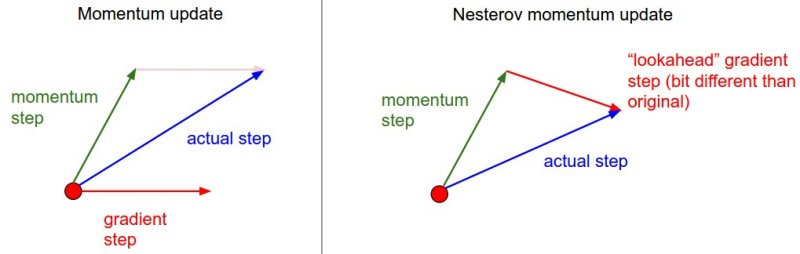
\includegraphics[width = \textwidth]{../GD/nesterov.jpeg}
   \caption{Ý tưởng của Nesterov accelerated gradient. (Nguồn: \href{href="http://cs231n.github.io/neural-networks-3/}{CS231n Stanford: Convolutional Neural Networks for Visual Recognition}}
   \label{fig:}
 \end{figure}

\begin{itemize}
    \item Với momentum thông thường: \textit{lượng thay đổi} là tổng của hai vector: momentum vector và gradient ở thời điểm hiện tại. 

    \item Với Nesterove momentum: \textit{lượng thay đổi} là tổng của hai vector: momentum vector và gradient ở thời điểm được xấp xỉ là điểm tiếp theo.  
\end{itemize}
 
 
\subsubsection{Công thức cập nhật}
 
Công thức cập nhật của NAG được cho như sau: 
 
\begin{eqnarray*} 
v_{t} &=& \gamma v_{t-1} + \eta \nabla_{\theta}J(\theta - \gamma v_{t-1}) \\\ 
\theta &=& \theta -  v_{t} 
\end{eqnarray*} 
 
Để ý một chút các bạn sẽ thấy điểm được tính đạo hàm đã thay đổi.  
 
 
\subsubsection{Ví dụ minh họa }
 
Dưới đây là ví dụ so sánh Momentum và NAG cho bài toán Linear Regression: 
 
% <div> 
% <table width = "100%" style = "border: 0px solid white"> 
%    <tr > 
%         <td width="40%" style = "border: 0px solid white">  
%         <img style="display:block;" width = "100%" src = "/assets/GD/LR_momentum_contours.gif"> 
%          </td> 
%         <td width="40%" style = "border: 0px solid white"> 
%         <img style="display:block;" width = "100%" src = "/assets/GD/LR_NAG_contours.gif"> 
%         </td> 
%     </tr> 
% </table>  
% <div class = "thecap"> Minh họa thuật toán GD với Momentum và NAG. </div> 
% </div> 
 
Hình bên trái là đường đi của nghiệm với phương pháp Momentum. nghiệm đi khá là \textit{zigzag} và mất nhiều vòng lặp hơn. Hình bên phải là đường đi của nghiệm với phương pháp NAG, nghiệm hội tụ nhanh hơn, và đường đi ít \textit{zigzag} hơn.  
 
(Source code cho \href{https://github.com/tiepvupsu/tiepvupsu.github.io/blob/master/assets/GD/LR%20Momentum.ipynb}{hình bên trái} và \href{https://github.com/tiepvupsu/tiepvupsu.github.io/blob/master/assets/GD/LR%20NAG.ipynb}{ hình bên phải}). 
 
 
\subsection{Các thuật toán khác}
Ngoài hai thuật toán trên, có rất nhiều thuật toán nâng cao khác được sử dụng trong các bài toán thực tế, đặc biệt là các bài toán Deep Learning. Có thể nêu một vài từ khóa như Adagrad, Adam, RMSprop,... Tôi sẽ không đề cập đến các thuật toán đó trong bài này mà sẽ dành thời gian nói tới nếu có dịp trong tương lai, khi blog đã đủ lớn và đã trang bị cho các bạn một lượng kiến thức nhất định.  
 
Tuy nhiên, bạn đọc nào muốn đọc thêm có thể tìm được rất nhiều thông tin hữu ích trong bài này: 
\href{http://sebastianruder.com/optimizing-gradient-descent/index.html#stochasticgradientdescent}{An overview of gradient descent optimization algorithms }. 
 
 
\section{Biến thể của Gradient Descent}
Tôi xin một lần nữa dùng bài toán \href{http://machinelearningcoban.com/2016/12/28/linearregression/}{Linear Regression} làm ví dụ. Hàm mất mát và đạo hàm của nó cho bài toán này lần lượt là (để cho thuận tiện, trong bài này tôi sẽ dùng ký hiệu $\mathbf{X}$ thay cho dữ liệu mở rộng $\bar{\mathbf{X}}$): 
 
\begin{equation*} 
J(\mathbf{w}) = \frac{1}{2N}\|\|\mathbf{X}\mathbf{w} - \mathbf{y}\|\|_2^2 
\end{equation*} 
\begin{equation*} 
~~~~ = \frac{1}{2N} \sum_{i=1}^N(\mathbf{x}_i \mathbf{w} - y_i)^2 
\end{equation*} 
và: 
\begin{equation*} 
\nabla_{\mathbf{w}} J(\mathbf{w}) = \frac{1}{N}\sum_{i=1}^N \mathbf{x}_i^T(\mathbf{x}_i\mathbf{w} - y_i) 
\end{equation*} 
 
 
\subsection{Batch Gradient Descent }
Thuật toán Gradient Descent chúng ta nói từ đầu phần 1 đến giờ còn được gọi là Batch Gradient Descent. Batch ở đây được hiểu là \textit{tất cả}, tức khi cập nhật $\theta = \mathbf{w}$, chúng ta sử dụng \textbf{tất cả} các điểm dữ liệu $\mathbf{x}_i$.  
 
Cách làm này có một vài hạn chế đối với cơ sở dữ liệu có vô cùng nhiều điểm (hơn 1 tỉ người dùng của facebook chẳng hạn). Việc phải tính toán lại đạo hàm với tất cả các điểm này sau mỗi vòng lặp trở nên cồng kềnh và không hiệu quả. Thêm nữa, thuật toán này được coi là không hiệu quả với \textit{online learning}. 
 
 
\textbf{Online learning} là khi cơ sở dữ liệu được cập nhật liên tục (thêm người dùng đăng ký hàng ngày chẳng hạn), mỗi lần thêm vài điểm dữ liệu mới. Kéo theo đó là mô hình của chúng ta cũng phải thay đổi một chút để phù hợp với các dữ liệu mới này. Nếu làm theo Batch Gradient Descent, tức tính lại đạo hàm của hàm mất mát tại tất cả các điểm dữ liệu, thì thời gian tính toán sẽ rất lâu, và thuật toán của chúng ta coi như không \textit{online} nữa do mất quá nhiều thời gian tính toán. 
 
Trên thực tế, có một thuật toán đơn giản hơn và tỏ ra rất hiệu quả, có tên gọi là Stochastic Gradient Descent (SGD). 
 
\subsection{Stochastic Gradient Descent.}
Trong thuật toán này, tại 1 thời điểm, ta chỉ tính đạo hàm của hàm mất mát dựa trên \textit{chỉ một} điểm dữ liệu $\mathbf{x_i}$ rồi cập nhật $\theta$ dựa trên đạo hàm này. Việc này được thực hiện với từng điểm trên toàn bộ dữ liệu, sau đó lặp lại quá trình trên. Thuật toán rất đơn giản này trê thực tế lại làm việc rất hiệu quả.  
 
Mỗi lần duyệt một lượt qua \textit{tất cả} các điểm trên toàn bộ dữ liệu được gọi là một epoch. Với GD thông thường thì mỗi epoch ứng với 1 lần cập nhật $\theta$, với SGD thì mỗi epoch ứng với $N$ lần cập nhật $\theta$ với $N$ là số điểm dữ liệu. Nhìn vào một mặt, việc cập nhật từng điểm một như thế này có thể làm giảm đi tốc độ thực hiện 1 epoch. Nhưng nhìn vào một mặt khác, SDG chỉ yêu cầu một lượng epoch rất nhỏ (thường là 10 cho lần đầu tiên, sau đó khi có dữ liệu mới thì chỉ cần chạy dưới một epoch là đã có nghiệm tốt). Vì vậy SGD phù hợp với các bài toán có lượng cơ sở dữ liệu lớn (chủ yếu là Deep Learning mà chúng ta sẽ thấy trong phần sau của blog) và các bài toán yêu cầu mô hình thay đổi liên tục, tức online learning. 
 
\textbf{Thứ tự lựa chọn điểm dữ liệu} 
 
Một điểm cần lưu ý đó là: sau mỗi epoch, chúng ta cần shuffle (xáo trộn) thứ tự của các dữ liệu để đảm bảo tính ngẫu nhiên. Việc này cũng ảnh hưởng tới hiệu năng của SGD.  
 
 
Một cách toán học, quy tắc cập nhật của SGD là: 
\begin{equation*} 
\theta = \theta - \eta \nabla_{\theta} J(\theta; \mathbf{x}_i; \mathbf{y}_i) 
\end{equation*} 
 
trong đó $J(\theta; \mathbf{x}_i; \mathbf{y}_i)$ là hàm mất mát với chỉ 1 cặp điểm dữ liệu (input, label) là ($\mathbf{x}_i, \mathbf{y}_i$). \textbf{Chú ý:} chúng ta hoàn toàn có thể áp dụng các thuật toán tăng tốc GD như Momentum, AdaGrad,... vào SGD. 
 
 
\subsubsection{Ví dụ với bài toán Linear Regression}
Với bài toán Linear Regression, $\theta = \mathbf{w}$, hàm mất mát tại một điểm dữ liệu là: 
\begin{equation*} 
J(\mathbf{w}; \mathbf{x}_i; y_i) = \frac{1}{2}(\mathbf{x}_i \mathbf{w} - y_i)^2 
\end{equation*} 
Đạo hàm theo $\mathbf{w}$ tương ứng là: 
\begin{equation*} 
\nabla_{\mathbf{w}}J(\mathbf{w}; \mathbf{x}_i; y_i) = \mathbf{x}_i^T(\mathbf{x}_i \mathbf{w} - y_i)^2 
\end{equation*} 
Và dưới đây là hàm số trong python để giải Linear Regression theo SGD: 
 
 
 
 
 
 
\begin{lstlisting}[language=Python]
# single point gradient 
def sgrad(w, i, rd_id): 
    true_i = rd_id[i] 
    xi = Xbar[true_i, :] 
    yi = y[true_i] 
    a = np.dot(xi, w) - yi 
    return (xi*a).reshape(2, 1) 
 
def SGD(w_init, grad, eta): 
    w = [w_init] 
    w_last_check = w_init 
    iter_check_w = 10 
    N = X.shape[0] 
    count = 0 
    for it in range(10): 
        # shuffle data  
        rd_id = np.random.permutation(N) 
        for i in range(N): 
            count += 1  
            g = sgrad(w[-1], i, rd_id) 
            w_new = w[-1] - eta*g 
            w.append(w_new) 
            if count%iter_check_w == 0: 
                w_this_check = w_new                  
                if np.linalg.norm(w_this_check - w_last_check)/len(w_init) < 1e-3:                                     
                    return w 
                w_last_check = w_this_check 
    return w 
\end{lstlisting}
 
Kết quả được cho như hình dưới đây (\href{http://machinelearningcoban.com/2017/01/12/gradientdescent/#quay-lai-voi-bai-toan-linear-regression}{với dữ liệu được tạo giống như ở phần 1}). 
 
<div> 
<table width = "100%" style = "border: 0px solid white"> 
   <tr > 
        <td width="40%" style = "border: 0px solid white">  
        <img style="display:block;" width = "100%" src = "/assets/GD/LR_SGD_contours.gif"> 
         </td> 
        <td width="40%" style = "border: 0px solid white"> 
        <img style="display:block;" width = "100%" src = "/assets/GD/LR_SGD_loss.png"> 
        </td> 
    </tr> 
</table>  
<div class = "thecap"> Trái: đường đi của nghiệm với SGD. Phải: giá trị của loss function tại 50 vòng lặp đầu tiên. </div> 
</div> 
 
Hình bên trái mô tả đường đi của nghiệm. Chúng ta thấy rằng đường đi khá là \textit{zigzag} chứ không \textit{mượt} như khi sử dụng GD. Điều này là dễ hiểu vì một điểm dữ liệu không thể đại diện cho toàn bộ dữ liệu được. Tuy nhiên, chúng ta cũng thấy rằng thuật toán hội tụ khá nhanh đến vùng lân cận của nghiệm. Với 1000 điểm dữ liệu, SGD chỉ cần gần 3 epoches (2911 tương ứng với 2911 lần cập nhật, mỗi lần lấy 1 điểm). Nếu so với con số 49 vòng lặp (epoches) như kết quả tốt nhất có được bằng GD, thì kết quả này lợi hơn rất nhiều.  
 
Hình bên phải mô tả hàm mất mát cho toàn bộ dữ liệu sau khi \textit{chỉ} sử dụng 50 điểm dữ liệu đầu tiên. Mặc dù không \textit{mượt}, tốc độ hội tụ vẫn rất nhanh.  
 
\textit{Thực tế cho thấy chỉ lấy khoảng 10 điểm là ta đã có thể xác định được gần đúng phương trình đường thẳng cần tìm rồi. Đây chính là ưu điểm của SGD - hội tụ rất nhanh.} 
 
 
\subsection{Mini-batch Gradient Descent}
Khác với SGD, mini-batch sử dụng một số lượng $n$ lớn hơn 1 (nhưng vẫn nhỏ hơn tổng số dữ liệu $N$rất nhiều). Giống với SGD, Mini-batch Gradient Descent bắt đầu mỗi epoch bằng việc xáo trộn ngẫu nhiên dữ liệu rồi chia toàn bộ dữ liệu thành các \textit{mini-batch}, mỗi \textit{mini-batch} có $n$ điểm dữ liệu (trừ mini-batch cuối có thể có ít hơn nếu $N$ không chia hết cho $n$). Mỗi lần cập nhật, thuật toán này lấy ra một mini-batch để tính toán đạo hàm rồi cập nhật. Công thức có thể viết dưới dạng: 
\begin{equation*} 
\theta = \theta - \eta\nabla_{\theta} J(\theta; \mathbf{x}_{i:i+n}; \mathbf{y}_{i:i+n}) 
\end{equation*} 
Với $\mathbf{x}_{i:i+n}$ được hiểu là dữ liệu từ thứ $i$ tới thứ $i+n-1$ (theo ký hiệu của Python). Dữ liệu này sau mỗi epoch là khác nhau vì chúng cần được xáo trộn. Một lần nữa, các thuật toán khác cho GD như Momentum, Adagrad, Adadelta,... cũng có thể được áp dụng vào đây. 
 
Mini-batch GD được sử dụng trong hầu hết các thuật toán Machine Learning, đặc biệt là trong Deep Learning. Giá trị $n$ thường được chọn là khoảng từ 50 đến 100. 
 
Dưới đây là ví dụ về giá trị của hàm mất mát mỗi khi cập nhật tham số $\theta$ của một bài toán khác phức tạp hơn. 
 
% <div class="imgcap"> 
%  <img src ="https://upload.wikimedia.org/wikipedia/commons/f/f3/Stogra.png" align = "center" width = "400"> 
%  <div class = "thecap"> Hàm mất mát <em>nhảy lên nhảy xuống</em> (fluctuate) sau mỗi lần cập nhật nhưng nhìn chung giảm dần và có xu hướng hội tụ về cuối. (Nguồn: <a href = "https://en.wikipedia.org/wiki/Stochastic_gradient_descent">Wikipedia</a>). </div> 
% </div> 
 
Để có thêm thông tin chi tiết hơn, bạn đọc có thể tìm trong \href{http://sebastianruder.com/optimizing-gradient-descent/index.html#stochasticgradientdescent}{bài viết rất tốt này}.  
 
 
 
 
\section{Stopping Criteria (điều kiện dừng)}
 
Có một điểm cũng quan trọng mà từ đầu tôi chưa nhắc đến: khi nào thì chúng ta biết thuật toán đã hội tụ và dừng lại? 
 
Trong thực nghiệm, có một vài phương pháp như dưới đây: 
 
1. Giới hạn số vòng lặp: đây là phương pháp phổ biến nhất và cũng để đảm bảo rằng chương trình chạy không quá lâu. Tuy nhiên, một nhược điểm của cách làm này là có thể thuật toán dừng lại trước khi đủ gần với nghiệm.  
2. So sánh gradient của nghiệm tại hai lần cập nhật liên tiếp, khi nào giá trị này đủ nhỏ thì dừng lại. Phương pháp này cũng có một nhược điểm lớn là việc tính đạo hàm đôi khi trở nên quá phức tạp (ví dụ như khi có quá nhiều dữ liệu), nếu áp dụng phương pháp này thì coi như ta không được lợi khi sử dụng SGD và mini-batch GD.  
3. So sánh giá trị của hàm mất mát của nghiệm tại hai lần cập nhật liên tiếp, khi nào giá trị này đủ nhỏ thì dừng lại. Nhược điểm của phương pháp này là nếu tại một thời điểm, đồ thị hàm số có dạng \textit{bẳng phẳng} tại một khu vực nhưng khu vực đó không chứa điểm local minimum (khu vực này thường được gọi là saddle points), thuật toán cũng dừng lại trước khi đạt giá trị mong muốn.  
4. Trong SGD và mini-batch GD, cách thường dùng là so sánh nghiệm sau một vài lần cập nhật. Trong đoạn code Python phía trên về SGD, tôi áp dụng việc so sánh này mỗi khi nghiệm được cập nhật 10 lần. Việc làm này cũng tỏ ra khá hiệu quả.  
 
 
 
 
\section{Một phương pháp tối ưu đơn giản khác: Newton's method}
 
Nhân tiện đang nói về tối ưu, tôi xin giới thiệu một phương pháp nữa có cách giải thích đơn giản: Newton's method. Các phương pháp GD tôi đã trình bày còn được gọi là first-order methods, vì lời giải tìm được dựa trên đạo hàm bậc nhất của hàm số. Newton's method là một second-order method, tức lời giải yêu cầu tính đến đạo hàm bậc hai. 
 
 
Nhắc lại rằng, cho tới thời điểm này, chúng ta luôn giải phương trình đạo hàm của hàm mất mát bằng 0 để tìm các điểm local minimun. (Và trong nhiều trường hợp, coi nghiệm tìm được là nghiệm của bài toán tìm giá trị nhỏ nhất của hàm mất mát). Có một thuật toán nối tiếng giúp giải bài toán $f(x) = 0$, thuật toán đó có tên là Newton's method. 
 
 
 
\subsection{Newton's method cho giải phương trình $f(x) = 0$}
 
Thuật toán Newton's method được mô tả trong hình động minh họa dưới đây: 
 
% <div class="imgcap"> 
%  <img src ="https://upload.wikimedia.org/wikipedia/commons/e/e0/NewtonIteration_Ani.gif" align = "center" width = "500"> 
%  <div class = "thecap"> Hình 3: Minh họa thuật toán Newton's method trong giải phương trình. (  Nguồn: <a href = "https://en.wikipedia.org/wiki/Newton's_method"> Newton's method - Wikipedia</a>).</div> 
% </div> 
 
 
Ý tưởng giải bài toán $f(x) = 0$ bằng phương pháp Newton's method như sau. Xuất phát từ một điểm $x_0$ được cho là gần với nghiệm $x^*$. Sau đó vẽ đường tiếp tuyến (mặt tiếp tuyến trong không gian nhiều chiều) với đồ thị hàm số $y = f(x)$ tại điểm trên đồ thị có hoành độ $x_0$. Giao điểm $x_1$ của đường tiếp tuyến này với trục hoành được xem là gần với nghiệm $x^*$ hơn. Thuật toán lặp lại với điểm mới $x_1$ và cứ như vậy đến khi ta được $f(x_t) \approx 0$. 
 
 
Đó là ý nghĩa hình học của Newton's method, chúng ta cần một công thức để có thể dựa vào đó để lập trình. Việc này không quá phức tạp với các bạn thi đại học môn toán ở VN. Thật vậy, phương trình tiếp tuyến với đồ thị của hàm $f(x)$ tại điểm có hoành độ $x_t$ là: 
\begin{equation*} 
y = f'(x_t)(x - x_t) + f(x_t) 
\end{equation*} 
Giao điểm của đường thẳng này với trục $x$ tìm được bằng cách giải phương trình vế phải của biểu thức trên bằng 0, tức là: 
\begin{equation*} 
x = x_t - \frac{f(x_t)}{f'(x_t)} \triangleq x_{t+1} 
\end{equation*} 
 
 
\subsection{Newton's method trong bài toán tìm local minimun}
Áp dụng phương pháp này cho việc giải phương trình $f'(x) = 0$ ta có: 
\begin{equation*} 
x_{t+1} = x_t -(f"(x_t))^{-1}{f'(x_t)} 
\end{equation*} 
 
Và trong không gian nhiều chiều với $\theta$ là biến: 
\begin{equation*} 
\theta = \theta - \mathbf{H}(J(\theta))^{-1} \nabla_{\theta} J(\theta) 
\end{equation*} 
trong đó $\mathbf{H}(J(\theta))$ là đạo hàm bậc hai của hàm mất mất (còn gọi là \href{https://en.wikipedia.org/wiki/Hessian_matrix}{Hessian matrix}). Biểu thức này là một ma trận nếu $\theta$ là một vector. Và $\mathbf{H}(J(\theta))^{-1}$ chính là nghịch đảo của ma trận đó.  
 
 
 
\subsection{Hạn chế của Newton's method}
\begin{itemize}
    \item Điểm khởi tạo phải \textit{rất} gần với nghiệm $x^*$. 
Ý tưởng sâu xa hơn của Newton's method là dựa trên khai triển Taylor của hàm số $f(x)$ tới đạo hàm thứ nhất: 
\begin{equation*} 
0 = f(x^\}) \approx f(x_t) + f'(x_t)(x_t - x^\}) 
\end{equation*} 
Từ đó suy ra: $x^\} \approx x_t - \frac{f(x_t)}{f'(x_t)}$.  
Một điểm rất quan trọng, khai triển Taylor chỉ đúng nếu $x_t$ rất gần với $x^*$! 
Dưới đây là một ví dụ kinh điển trên Wikipedia về việc Newton's method cho một dãy số phân kỳ (divergence). 
% <div class="imgcap"> 
%  <img src ="https://upload.wikimedia.org/wikipedia/commons/thumb/f/f1/NewtonsMethodConvergenceFailure.svg/300px-NewtonsMethodConvergenceFailure.svg.png" align = "center" width = "400"> 
%  <div class = "thecap"> Hình 4: Nghiệm là một điểm gần -2. Tiếp tuyến của đồ thị hàm số tại điểm có hoành độ bằng 0 cắt trục hoành tại 1, và ngược lại. Trong trường hợp này, Newton's method không bao giờ hội tụ. (Nguồn: <a href = "https://en.wikipedia.org/wiki/Newton's_method">Wikipedia</a>). </div> 
% </div> 


\item Nhận thấy rằng trong việc giải phương trình $f(x) = 0$, chúng ta có đạo hàm ở mẫu số. Khi đạo hàm này gần với 0, ta sẽ được một đường thằng song song hoặc gần song song với trục hoành. Ta sẽ hoặc không tìm được giao điểm, hoặc được một giao điểm ở vô cùng. Đặc biệt, khi nghiệm chính là điểm có đạo hàm bằng 0, thuật toán gần như sẽ không tìm được nghiệm! 

 \item Khi áp dụng Newton's method cho bài toán tối ưu trong không gian nhiều chiều, chúng ta cần tính nghịch đảo của Hessian matrix. Khi số chiều và số điểm dữ liệu lớn, đạo hàm bậc hai của hàm mất mát sẽ là một ma trận rất lớn, ảnh hưởng tới cả memory và tốc độ tính toán của hệ thống. 

\end{itemize}
 
\section{Kết luận}
Qua hai bài viết về Gradient Descent này, tôi hy vọng các bạn đã hiểu và làm quen với một thuật toán tối ưu được sử dụng nhiều nhất trong Machine Learning và đặc biệt là Deep Learning. Còn nhiều biến thể khác khá thú vị về GD (mà rất có thể tôi chưa biết tới), nhưng tôi xin phép được dừng chuỗi bài về GD tại đây và tiếp tục chuyển sang các thuật toán thú vị khác.  
 
Hy vọng bài viết có ích với các bạn. 
 
 
\section{Tài liệu tham khảo}
 
[1] \href{https://en.wikipedia.org/wiki/Newton's_method}{Newton's method - Wikipedia} 
 
[2] \href{http://sebastianruder.com/optimizing-gradient-descent/index.html#stochasticgradientdescent}{An overview of gradient descent optimization algorithms} 
 
[3] \href{https://en.wikipedia.org/wiki/Stochastic_gradient_descent}{Stochastic Gradient Descent - Wikipedia} 
 
[4] \href{https://www.youtube.com/watch?v=UfNU3Vhv5CA}{Stochastic Gradient Descen - Andrew Ng}  
 
[5] Nesterov, Y. (1983). A method for unconstrained convex minimization problem with the rate of convergence o(1/k2). Doklady ANSSSR (translated as Soviet.Math.Docl.), vol. 269, pp. 543– 547. 

%!TEX root = book.tex
\chapter{Perceptron Learning Algorithm}
--- 
 
Cứ làm đi, sai đâu sửa đấy, cuối cùng sẽ thành công! 
 
Đó chính là ý tưởng chính của một thuật toán rất quan trọng trong Machine Learning - thuật toán Perceptron Learning Algorithm hay PLA. 

 
\section{Giới thiệu}
 
Trong bài này, tôi sẽ giới thiệu thuật toán đầu tiên trong Classification có tên là Perceptron Learning Algorithm (PLA) hoặc đôi khi được viết gọn là Perceptron.  
 
Perceptron là một thuật toán Classification cho trường hợp đơn giản nhất: chỉ có hai class (lớp) (\textit{bài toán với chỉ hai class được gọi là binary classification}) và cũng chỉ hoạt động được trong một trường hợp rất cụ thể. Tuy nhiên, nó là nền tảng cho một mảng lớn quan trọng của Machine Learning là Neural Networks và sau này là Deep Learning. (Tại sao lại gọi là Neural Networks - tức mạng dây thần kinh - các bạn sẽ được thấy ở cuối bài). 
 
Giả sử chúng ta có hai tập hợp dữ liệu đã được gán nhãn được minh hoạ trong Hình 1 bên trái dưới đây. Hai class của chúng ta là tập các điểm màu xanh và tập các điểm màu đỏ. Bài toán đặt ra là: từ dữ liệu của hai tập được gán nhãn cho trước, hãy xây dựng một \textit{classifier} (bộ phân lớp) để khi có một điểm dữ liệu hình tam giác màu xám mới, ta có thể dự đoán được màu (nhãn) của nó.  
 
<table width = "100%" style = "border: 0px solid white"> 
   <tr > 
        <td width="40%" style = "border: 0px solid white">  
        <img style="display:block;" width = "100%" src = "/assets/pla/pla1.png"> 
         </td> 
        <td width="40%" style = "border: 0px solid white"> 
        <img style="display:block;" width = "100%" src = "/assets/pla/pla2.png"> 
        </td> 
    </tr> 
</table>  
<div class = "thecap">Hình 1: Bài toán Perceptron</div> 
 
Hiểu theo một cách khác, chúng ta cần tìm \textit{lãnh thổ} của mỗi class sao cho, với mỗi một điểm mới, ta chỉ cần xác định xem nó nằm vào lãnh thổ của class nào rồi quyết định nó thuộc class đó. Để tìm \textit{lãnh thổ} của mỗi class, chúng ta cần đi tìm biên giới (boundary) giữa hai \textit{lãnh thổ} này. Vậy bài toán classification có thể coi là bài toán đi tìm boundary giữa các class. Và boundary đơn giản nhât trong không gian hai chiều là một đường thằng, trong không gian ba chiều là một mặt phẳng, trong không gian nhiều chiều là một siêu mặt phẳng (hyperplane) (tôi gọi chung những boundary này là \textit{đường phẳng}). Những boundary phẳng này được coi là đơn giản vì nó có thể biểu diễn dưới dạng toán học bằng một hàm số đơn giản có dạng tuyến tính, tức linear. Tất nhiên, chúng ta đang giả sử rằng tồn tại một đường phẳng để có thể phân định \textit{lãnh thổ} của hai class. Hình 1 bên phải minh họa một đường thẳng phân chia hai class trong mặt phẳng. Phần có nền màu xanh được coi là \textit{lãnh thổ} của lớp xanh, phần có nên màu đỏ được coi là \textit{lãnh thổ} của lớp đỏ. Trong trường hợp này, điểm dữ liệu mới hình tam giác được phân vào class đỏ.  
 
 
\subsection{Bài toán Perceptron }
Bài toán Perceptron được phát biểu như sau: \textit{Cho hai class được gán nhãn, hãy tìm một đường phẳng sao cho toàn bộ các điểm thuộc class 1 nằm về 1 phía, toàn bộ các điểm thuộc class 2 nằm về phía còn lại của đường phẳng đó. Với giả định rằng tồn tại một đường phẳng như thế.} 
 
Nếu tồn tại một đường phẳng phân chia hai class thì ta gọi hai class đó là \textit{linearly separable}. Các thuật toán classification tạo ra các boundary là các đường phẳng được gọi chung là Linear Classifier. 
 
 
\section{Thuật toán Perceptron (PLA)}
Cũng giống như các thuật toán lặp trong \href{http://machinelearningcoban.com/2017/01/01/kmeans/}{K-means Clustering} và \href{http://machinelearningcoban.com/2017/01/12/gradientdescent/}{Gradient Descent}, ý tưởng cơ bản của PLA là xuất phát từ một nghiệm dự đoán nào đó, qua mỗi vòng lặp, nghiệm sẽ được cập nhật tới một ví trí tốt hơn. Việc cập nhật này dựa trên việc giảm giá trị của một hàm mất mát nào đó.  
 
 
\subsection{Một số ký hiệu}
Giả sử $\mathbf{X} = [\mathbf{x}_1, \mathbf{x}_2, \dots, \mathbf{x}_N] \in \mathbb{R}^{d \times N}$ là ma trận chứa các điểm dữ liệu mà mỗi cột $\mathbf{x}_i \in \mathbb{R}^{d\times 1}$ là một điểm dữ liệu trong không gian $d$ chiều. (\textit{Chú ý: khác với các bài trước tôi thường dùng các vector hàng để mô tả dữ liệu, trong bài này tôi dùng vector cột để biểu diễn. Việc biểu diễn dữ liệu ở dạng hàng hay cột tùy thuộc vào từng bài toán, miễn sao cách biễu diễn toán học của nó khiến cho người đọc thấy dễ hiểu}). 
 
Giả sử thêm các nhãn tương ứng với từng điểm dữ liệu được lưu trong một vector hàng $\mathbf{y} = [y_1, y_2, \dots, y_N] \in \mathbb{R}^{1\times N}$, với $y_i = 1$ nếu $\mathbf{x}_i$ thuộc class 1 (xanh) và $y_i = -1$ nếu $\mathbf{x}_i$ thuộc class 2 (đỏ). 
 
Tại một thời điểm, giả sử ta tìm được boundary là đường phẳng có phương trình: 
\begin{eqnarray} 
f_{\mathbf{w}}(\mathbf{x}) &=& w_1x_1 + \dots + w_dx_d + w_0 \\\  
&=&\mathbf{w}^T\mathbf{\bar{x}} = 0 
\end{eqnarray} 
 
với $\mathbf{\bar{x}}$ là điểm dữ liệu mở rộng bằng cách thêm phần tử $x_0 = 1$ lên trước vector $\mathbf{x}$ tương tự như trong \href{http://machinelearningcoban.com/2016/12/28/linearregression/}{Linear Regression}. Và từ đây, khi nói $\mathbf{x}$, tôi cũng ngầm hiểu là điểm dữ liệu mở rộng. 
 
Để cho đơn giản, chúng ta hãy cùng làm việc với trường hợp mỗi điểm dữ liệu có số chiều $d = 2$. Giả sử đường thẳng $w_1 x_1 + w_2 x_2 + w_0 = 0$ chính là nghiệm cần tìm như Hình 2 dưới đây: 
 
% <div class="imgcap"> 
% <img src ="\assets\pla\pla4.png" align = "center" width = "400"> 
% <div class = "thecap">Hình 2: Phương trình đường thẳng boundary.</div> 
% </div>  
 
Nhận xét rằng các điểm nằm về cùng 1 phía so với đường thẳng này sẽ làm cho hàm số $f_{\mathbf{w}}(\mathbf{x})$ mang cùng dấu. Chỉ cần đổi dấu của $\mathbf{w}$ nếu cần thiết, ta có thể giả sử các điểm nằm trong nửa mặt phẳng nền xanh mang dấu dương (+), các điểm nằm trong nửa mặt phẳng nền đỏ mang dấu âm (-). Các dấu này cũng tương đương với nhãn $y$ của mỗi class. Vậy nếu $\mathbf{w}$ là một nghiệm của bài toán Perceptron, với một điểm dữ liệu mới $\mathbf{x}$ chưa được gán nhãn, ta có thể xác định class của nó bằng phép toán đơn giản như sau: 
\begin{equation*} 
\text{label}(\mathbf{x}) = 1 ~\text{if}~ \mathbf{w}^T\mathbf{x} \geq 0, \text{otherwise} -1 
\end{equation*} 
 
Ngắn gọn hơn:  
\begin{equation*} 
\text{label}(\mathbf{x}) = \text{sgn}(\mathbf{w}^T\mathbf{x}) 
\end{equation*} 
trong đó, $\text{sgn}$ là hàm xác định dấu, với giả sử rằng $\text{sgn}(0) = 1$. 
 
 
\subsection{Xây dựng hàm mất mát}
Tiếp theo, chúng ta cần xây dựng hàm mất mát với tham số $\mathbf{w}$ bất kỳ. Vẫn trong không gian hai chiều, giả sử đường thẳng $w_1x_1 + w_2x_2 + w_0 = 0$ được cho như Hình 3 dưới đây: 
% <div class="imgcap"> 
% <img src ="\assets\pla\pla3.png" align = "center" width = "400"> 
% <div class = "thecap">Hình 3: Đường thẳng bất kỳ và các điểm bị misclassified được khoanh tròn.</div> 
% </div>  
 
Trong trường hợp này, các điểm được khoanh tròn là các điểm bị misclassified (phân lớp lỗi). Điều chúng ta mong muốn là không có điểm nào bị misclassified. Hàm mất mát đơn giản nhất chúng ta nghĩ đến là hàm \textit{đếm} số lượng các điểm bị misclassied và tìm cách tối thiểu hàm số này: 
\begin{equation*} 
J_1(\mathbf{w}) = \sum_{\mathbf{x}_i \in \mathcal{M}} (-y_i\text{sgn}(\mathbf{w}^T\mathbf{x_i})) 
\end{equation*} 
 
trong đó $\mathcal{M}$ là tập hợp các điểm bị misclassifed (\textit{tập hợp này thay đổi theo} $\mathbf{w}$). Với mỗi điểm $\mathbf{x}_i \in \mathcal{M}$, vì điểm này bị misclassified nên $y_i$ và $\text{sgn}(\mathbf{w}^T\mathbf{x})$ khác nhau, và vì thế $-y_i\text{sgn}(\mathbf{w}^T\mathbf{x_i}) = 1 $. Vậy $J_1(\mathbf{w})$ chính là hàm \textit{đếm} số lượng các điểm bị misclassified. Khi hàm số này đạt giá trị nhỏ nhất bằng 0 thì ta không còn điểm nào bị misclassified.  
 
Một điểm quan trọng, hàm số này là rời rạc, không tính được đạo hàm theo $\mathbf{w}$ nên rất khó tối ưu. Chúng ta cần tìm một hàm mất mát khác để việc tối ưu khả thi hơn. 
 
Xét hàm mất mát sau đây:  
 
\begin{equation*} 
J(\mathbf{w}) = \sum_{\mathbf{x}_i \in \mathcal{M}} (-y_i\mathbf{w}^T\mathbf{x_i}) 
\end{equation*} 
 
Hàm $J()$ khác một chút với hàm $J_1()$ ở việc bỏ đi hàm $\text{sgn}$. Nhận xét rằng khi một điểm misclassified $\mathbf{x}_i$ nằm càng xa boundary thì giá trị $-y_i\mathbf{w}^T\mathbf{x}_i$ sẽ càng lớn, nghĩa là sự sai lệch càng lớn. Giá trị nhỏ nhất của hàm mất mát này cũng bằng 0 nếu không có điểm nào bị misclassifed. Hàm mất mát này cũng được cho là tốt hơn hàm $J_1()$ vì hàm này \textit{trừng phạt} rất nặng những điểm \textit{lấn sâu sang lãnh thổ của class kia}. Trong khi đó, $J()$ \textit{trừng phạt} các điểm misclassified như nhau (đều = 1), bất kể chúng xa hay gần với đường biên giới. 
 
Tại một thời điểm, nếu chúng ta chỉ quan tâm tới các điểm bị misclassified thì hàm số $J(\mathbf{w})$ khả vi (tính được đạo hàm), vậy chúng ta có thể sử dụng \href{http://machinelearningcoban.com/2017/01/12/gradientdescent/}{Gradient Descent} hoặc \href{http://machinelearningcoban.com/2017/01/16/gradientdescent2/#-stochastic-gradient-descent}{Stochastic Gradient Descent (SGD)} để tối ưu hàm mất mát này. Với ưu điểm của SGD cho các bài toán \href{http://machinelearningcoban.com/2017/01/12/gradientdescent/#large-scale}{large-scale}, chúng ta sẽ làm theo thuật toán này.  
 
Với \textit{một} điểm dữ liệu $\mathbf{x}_i$ bị misclassified, hàm mất mát trở thành: 
 
\begin{equation*} 
J(\mathbf{w}; \mathbf{x}_i; y_i) = -y_i\mathbf{w}^T\mathbf{x}_i 
\end{equation*} 
 
Đạo hàm tương ứng: 
 
\begin{equation*} 
\nabla_{\mathbf{w}}J(\mathbf{w}; \mathbf{x}_i; y_i) = -y_i\mathbf{x}_i 
\end{equation*} 
Vậy quy tắc cập nhật là: 
\begin{equation*} 
\mathbf{w} = \mathbf{w} + \eta y_i\mathbf{x}_i 
\end{equation*} 
với $\eta$ là learning rate.  
 
Nhận xét rằng nếu $\mathbf{w}$ là nghiệm thì $\eta\mathbf{w}$ cũng là nghiệm với $\eta$ là một số khác 0 bất kỳ. Vậy nếu $\mathbf{w}_0$ nhỏ gần với 0 và số vòng lặp đủ lớn, ta có thể coi như learning rate $\eta = 1$. Ta có một quy tắc cập nhật rất gọn là: $\mathbf{w}_{t+1} = \mathbf{w}_{t} + y_i\mathbf{x}_i$. Nói cách khác, với mỗi điểm $\mathbf{x}_i$ bị misclassifed, ta chỉ cần nhân điểm đó với nhãn $y_i$ của nó, lấy kết quả cộng vào $\mathbf{w}$ ta sẽ được $\mathbf{w}$ mới. 
 
Ta có một quan sát nhỏ ở đây: 
\begin{equation*} 
\mathbf{w}_{t+1}^T\mathbf{x}_i = (\mathbf{w}_{t} + y_i\mathbf{x}_i)^T\mathbf{x}_{i} \\\ 
= \mathbf{w}_{t}^T\mathbf{x}_i + y_i \|\|\mathbf{x}_i\|\|_2^2 
\end{equation*} 
 
Nếu $y_i = 1$, vì $\mathbf{x}_i$ bị misclassifed nên $\mathbf{w}_{t}^T\mathbf{x}_i < 0$. Cũng vì $y_i = 1$ nên $y_i \|\|\mathbf{x}_i\|\|_2^2 = \|\|\mathbf{x}_i\|\|_2^2 \geq 1$ (chú ý $x_0 = 1$), nghĩa là $\mathbf{w}_{t+1}^T\mathbf{x}_i > \mathbf{w}_{t}^T\mathbf{x}_i$. Lý giải bằng lời, $\mathbf{w}_{t+1}$ tiến về phía làm cho $\mathbf{x}_i$ được phân lớp đúng. Điều tương tự xảy ra nếu $y_i = -1$. 
 
Đến đây, cảm nhận của chúng ta với thuật toán này là: cứ chọn đường boundary đi. Xét từng điểm một, nếu điểm đó bị misclassified thì tiến đường boundary về phía làm cho điểm đó được classifed đúng. Có thể thấy rằng, khi di chuyển đường boundary này, các điểm trước đó được classified đúng có thể lại bị misclassified. Mặc dù vậy, PLA vẫn được đảm bảo sẽ hội tụ sau một số hữu hạn bước (tôi sẽ chứng minh việc này ở phía sau của bài viết). Tức là cuối cùng, ta sẽ tìm được đường phẳng phân chia hai lớp, miễn là hai lớp đó là linearly separable. Đây cũng chính là lý do câu đầu tiên trong bài này tôi nói với các bạn là: "Cứ làm đi, sai đâu sửa đấy, cuối cùng sẽ thành công!". 
 
Tóm lại, thuật toán Perceptron có thể được viết như sau: 
 
 
\subsection{Tóm tắt PLA }
 
1. Chọn ngẫu nhiên một vector hệ số $\mathbf{w}$ với các phần tử gần 0. 
2. Duyệt ngẫu nhiên qua từng điểm dữ liệu $\mathbf{x}_i$: 
    \begin{itemize}
        \item Nếu $\mathbf{x}_i$ được phân lớp đúng, tức $\text{sgn}(\mathbf{w}^T\mathbf{x}) = y_i$, chúng ta không cần làm gì. 

        \item Nếu $\mathbf{x}_i$ bị misclassifed, cập nhật $\mathbf{w}$ theo công thức: 
    \end{itemize}
    \begin{equation*} 
    \mathbf{w} = \mathbf{w} + y_i\mathbf{x}_i 
    \end{equation*} 
3. Kiểm tra xem có bao nhiêu điểm bị misclassifed. Nếu không còn điểm nào, dừng thuật toán. Nếu còn, quay lại bước 2. 
 
 
 
 
\section{Ví dụ trên Python}
Như thường lệ, chúng ta sẽ thử một ví dụ nhỏ với Python. 
 
 
\subsection{Load thư viện và tạo dữ liệu}
Chúng ta sẽ tạo hai nhóm dữ liệu, mỗi nhóm có 10 điểm, mỗi điểm dữ liệu có hai chiều để thuận tiện cho việc minh họa. Sau đó, tạo dữ liệu mở rộng bằng cách thêm 1 vào đầu mỗi điểm dữ liệu.  
 
 
\begin{lstlisting}[language=Python]
# generate data 
# list of points  
import numpy as np  
import matplotlib.pyplot as plt 
from scipy.spatial.distance import cdist 
np.random.seed(2) 
 
means = [[2, 2], [4, 2]] 
cov = [[.3, .2], [.2, .3]] 
N = 10 
X0 = np.random.multivariate_normal(means[0], cov, N).T 
X1 = np.random.multivariate_normal(means[1], cov, N).T 
 
X = np.concatenate((X0, X1), axis = 1) 
y = np.concatenate((np.ones((1, N)), -1*np.ones((1, N))), axis = 1) 
# Xbar  
X = np.concatenate((np.ones((1, 2*N)), X), axis = 0) 
\end{lstlisting}
 
Sau khi thực hiện đoạn code này, biến \pythoninline{X} sẽ chứa dữ liệu input (mở rộng), biến \pythoninline{y} sẽ chứa nhãn của mỗi điểm dữ liệu trong \pythoninline{X}. 
 
\subsection{Các hàm số cho PLA}
Tiếp theo chúng ta cần viết 3 hàm số cho PLA: 
 
1. \pythoninline{h(w, x)}: tính đầu ra khi biết đầu vào \pythoninline{x} và weights \pythoninline{w}. 
2. \pythoninline{has_converged(X, y, w)}: kiểm tra xem thuật toán đã hội tụ chưa. Ta chỉ cần so sánh \pythoninline{h(w, X)} với \textit{ground truth} \pythoninline{y}. Nếu giống nhau thì dừng thuật toán. 
3. \pythoninline{perceptron(X, y, w_init)}: hàm chính thực hiện PLA. 
 
\begin{lstlisting}[language=Python]
def h(w, x):     
    return np.sign(np.dot(w.T, x)) 
 
def has_converged(X, y, w):     
    return np.array_equal(h(w, X), y)  
 
def perceptron(X, y, w_init): 
    w = [w_init] 
    N = X.shape[1] 
    d = X.shape[0] 
    mis_points = [] 
    while True: 
        # mix data  
        mix_id = np.random.permutation(N) 
        for i in range(N): 
            xi = X[:, mix_id[i]].reshape(d, 1) 
            yi = y[0, mix_id[i]] 
            if h(w[-1], xi)[0] != yi: # misclassified point 
                mis_points.append(mix_id[i]) 
                w_new = w[-1] + yi*xi  
                w.append(w_new) 
                 
        if has_converged(X, y, w[-1]): 
            break 
    return (w, mis_points) 
 
d = X.shape[0] 
w_init = np.random.randn(d, 1) 
(w, m) = perceptron(X, y, w_init) 
\end{lstlisting}
 
Dưới đây là hình minh họa thuật toán PLA cho bài toán nhỏ này: 
 
% <div class="imgcap"> 
% <img src ="\assets\pla\pla_vis.gif" align = "center" width = "400"> 
% <div class = "thecap"> Hình 4: Minh họa thuật toán PLA </div> 
% </div>  
Sau khi cập nhật 18 lần, PLA đã hội tụ. Điểm được khoanh tròn màu đen là điểm misclassified tương ứng được chọn để cập nhật đường boundary.  
 
Source code cho phần này (bao gồm hình động) \href{https://github.com/tiepvupsu/tiepvupsu.github.io/blob/master/assets/pla/perceptron.py}{có thể được tìm thấy ở đây}. 
 
 
\section{Chứng minh hội tụ}
 
Giả sử rằng $\mathbf{w}^*$ là một nghiệm của bài toán (ta có thể giả sử việc này được vì chúng ta đã có giả thiết hai class là linearly separable - tức tồn tại nghiệm). Có thể thấy rằng, với mọi $\alpha > 0$, nếu $\mathbf{w}^*$ là nghiệm, $\alpha\mathbf{w}^*$ cũng là nghiệm của bài toán. Xét dãy số không âm $ u_{\alpha}(t) = \|\|\mathbf{w}_{t} - \alpha\mathbf{w}^*\|\|_2^2$. Với $\mathbf{x}_i$ là một điểm bị misclassified nếu dùng nghiệm $\mathbf{w}_t$ ta có:  
 
 
 
 
\begin{eqnarray} 
&&u_{\alpha}(t+1) = \|\|\mathbf{w}_{t+1} - \alpha \mathbf{w}^*\|\|_2^2 \\\ 
&=& \|\|\mathbf{w}_{t} + y_i\mathbf{x}_i - \alpha\mathbf{w}^*\|\|_2^2 \\\ 
&=& \|\|\mathbf{w}_{t} -\alpha\mathbf{w}^*\|\|_2^2 + y_i^2\|\|\mathbf{x}_i\|\|_2^2 + 2y_i\mathbf{x}_i^T(\mathbf{w} - \alpha\mathbf{w}^*) \\\ 
&<& u_{\alpha}(t) \ + \|\|\mathbf{x}_i\|\|_2^2 - 2\alpha y_i\mathbf{x}_i^T \mathbf{w}^\} 
\end{eqnarray} 
 
 
Dấu nhỏ hơn ở dòng cuối là vì $y_i^2 = 1$ và $2y_i\mathbf{x}_i^T\mathbf{w}_{t} < 0$. Nếu ta đặt:  
 
\begin{eqnarray} 
\beta^2 &=& \max_{i=1, 2, \dots, N}\|\|\mathbf{x}_i\|\|_2^2 \\\ 
\gamma &=& \min_{i=1, 2, \dots, N} y_i\mathbf{x}_i^T\mathbf{w}^\} 
\end{eqnarray} 
 
và chọn $\alpha = \frac{\beta^2}{\gamma}$, ta có: 
\begin{equation*} 
0 \leq u_{\alpha}(t+1) < u_{\alpha}(t) + \beta^2 - 2\alpha\gamma = u_{\alpha}(t) - \beta^2 
\end{equation*} 
 
Điều này nghĩa là: nếu luôn luôn có các điểm bị misclassified thì dãy $u_{\alpha}(t)$ là dãy giảm, bị chặn dưới bởi 0, và phần tử sau kém phần tử trước ít nhất một lượng là $\beta^2>0$. Điều vô lý này chứng tỏ đến một lúc nào đó sẽ không còn điểm nào bị misclassified. Nói cách khác, thuật toán PLA hội tụ sau một số hữu hạn bước.  
 
 
\section{Mô hình Neural Network đầu tiên}
Hàm số xác định class của Perceptron $\text{label}(\mathbf{x}) = \text{sgn}(\mathbf{w}^T\mathbf{x})$ có thể được mô tả như hình vẽ (được gọi là network) dưới đây: 
 
% <div class="imgcap"> 
% <img src ="\assets\pla\pla_nn.png" align = "center" width = "800"> 
% <div class = "thecap"> Hình 5: Biểu diễn của Perceptron dưới dạng Neural Network.</div> 
% </div>  
 
Đầu vào của network $\mathbf{x}$ được minh họa bằng các node màu xanh lục với node $x_0$ luôn luôn bằng 1. Tập hợp các node màu xanh lục được gọi là \textit{Input layer}. Trong ví dụ này, tôi giả sử số chiều của dữ liệu $d = 4$. Số node trong input layer luôn luôn là $d + 1$ với một node là 1 được thêm vào. Node $x_0 = 1$ này đôi khi được ẩn đi.  
 
Các trọng số (\textit{weights}) $w_0, w_1, \dots, w_d$ được gán vào các mũi tên đi tới node $\displaystyle z = \sum_{i=0}^dw_ix_i = \mathbf{w}^T\mathbf{x}$. Node $y = \text{sgn}(z)$ là \textit{output} của network. Ký hiệu hình chữ Z ngược màu xanh trong node $y$ thể hiện đồ thị của hàm số $\text{sgn}$.  
 
Trong thuật toán PLA, ta phải tìm các weights trên các mũi tên sao cho với mỗi $\mathbf{x}_i$ ở tập các điểm dữ liệu đã biết được đặt ở Input layer, output của network này trùng với nhãn $y_i$ tương ứng.  
 
Hàm số $y = \text{sgn}(z)$ còn được gọi là \textit{activation function}. Đây chính là dạng đơn giản nhất của Neural Network. 
 
 
Các Neral Networks sau này có thể có nhiều node ở output tạo thành một \textit{output layer}, hoặc có thể có thêm các layer trung gian giữa \textit{input layer} và \textit{output layer}. Các layer trung gian đó được gọi là \textit{hidden layer}. Khi biểu diễn các Networks lớn, người ta thường giản lược hình bên trái thành hình bên phải. Trong đó node $x_0 = 1$ thường được ẩn đi. Node $z$ cũng được ẩn đi và viết gộp vào trong node $y$. Perceptron thường được vẽ dưới dạng đơn giản như Hình 5 bên phải.  
 
Để ý rằng nếu ta thay \textit{activation function} bởi $y = z$, ta sẽ có Neural Network mô tả thuật toán Linear Regression như hình dưới. Với đường thẳng chéo màu xanh thể hiện đồ thị hàm số $y = z$. Các trục tọa độ đã được lược bỏ. 
 
% <div class="imgcap"> 
% <img src ="\assets\pla\lr_nn.png" align = "center" width = "300"> 
% <div class = "thecap"> Hình 6: Biểu diễn của Linear Regression dưới dang Neural Network.</div> 
% </div>  
 
 
 
 
 
 
Mô hình perceptron ở trên khá giống với một node nhỏ của dây thân kinh sinh học như hình sau đây: 
 
% <div class="imgcap"> 
% <img src ="http://sebastianraschka.com/images/blog/2015/singlelayer_neural_networks_files/perceptron_neuron.png" align = "center" width = "600"> 
% <div class = "thecap">Hình 7: Mô tả một neuron thần kinh sinh học. (Nguồn: <a href = "http://sebastianraschka.com/Articles/2015_singlelayer_neurons.html">Single-Layer Neural Networks and Gradient Descent</a>)</div> 
% </div>  
 
 
Dữ liệu từ nhiều dây thần kinh đi về một \textit{cell nucleus}. Thông tin được tổng hợp và được đưa ra ở output. Nhiều bộ phận như thế này kết hợp với nhau tạo nên hệ thần kinh sinh học. Chính vì vậy mà có tên Neural Networks trong Machine Learning. Đôi khi mạng này còn được gọi là Artificial Neural Networks (ANN) tức \textit{hệ neuron nhân tạo}.  
 
 
\section{Thảo Luận}
 
\subsection{PLA có thể cho vô số nghiệm khác nhau }
Rõ ràng rằng, nếu hai class là linearly separable thì có vô số đường thằng phân cách 2 class đó. Dưới đây là một ví dụ: 
 
<div class="imgcap"> 
<img src ="/assets/pla/pla6.png" align = "center" width = "400"> 
<div class = "thecap">Hình 8: PLA có thể cho vô số nghiệm khác nhau.</div> 
</div>  
 
Tất cả các đường thẳng màu đen đều thỏa mãn. Tuy nhiên, các đường khác nhau sẽ quyết định điểm hình tam giác thuộc các lớp khác nhau. Trong các đường đó, đường nào là tốt nhất? Và định nghĩa "tốt nhất" được hiểu theo nghĩa nào? Có một thuật toán khác định nghĩa và tìm đường tốt nhất như thế, tôi sẽ giới thiệu trong 1 vài bài tới. Mời các bạn đón đọc.  
 
 
\subsection{PLA đòi hỏi dữ liệu linearly separable}
 
Hai class trong ví dụ dưới đây \textit{tương đối} linearly separable. Mỗi class có 1 điểm coi như \textit{nhiễu} nằm trong khu vực các điểm của class kia. PLA sẽ không làm việc trong trường hợp này vì luôn luôn có ít nhất 2 điểm bị misclassified.  
 
<div class="imgcap"> 
<img src ="/assets/pla/pla7.png" align = "center" width = "400"> 
<div class = "thecap">Hinhf 9: PLA không làm việc nếu chỉ có một nhiễu nhỏ.</div> 
</div>  
 
Trong một chừng mực nào đó, đường thẳng màu đen vẫn có thể coi là một nghiệm tốt vì nó đã giúp phân loại chính xác hầu hết các điểm. Việc không hội tụ với dữ liệu \textit{gần} linearly separable chính là một nhược điểm lớn của PLA. 
 
Để khắc phục nhược điểm này, có một cải tiến nhỏ như thuật toán Pocket Algorithm dưới đây: 
 
\subsection{Pocket Algorithm}
Một cách tự nhiên, nếu có một vài \textit{nhiễu}, ta sẽ đi tìm một đường thẳng phân chia hai class sao cho có ít điểm bị misclassified nhất. Việc này có thể được thực hiện thông qua PLA với một chút thay đổi nhỏ như sau: 
 
1. Giới hạn số lượng vòng lặp của PLA. 
2. Mỗi lần cập nhật nghiệm $\mathbf{w}$ mới, ta đếm xem có bao nhiêu điểm bị misclassified. Nếu là lần đầu tiên, giữ lại nghiệm này trong \textit{pocket} (túi quần). Nếu không, so sánh số điểm misclassified này với số điểm misclassified của nghiệm trong \textit{pocket}, nếu nhỏ hơn thì \textit{lôi} nghiệm cũ ra, đặt nghiệm mới này vào.  
 
Thuật toán này giống với thuật toán tìm phần tử nhỏ nhất trong 1 mảng.  
 
 
\section{Kết luận}
 
Hy vọng rằng bài viết này sẽ giúp các bạn phần nào hiểu được một số khái niệm trong Neural Networks. Trong một số bài tiếp theo, tôi sẽ tiếp tục nói về các thuật toán cơ bản khác trong Neural Networks trước khi chuyển sang phần khác.  
 
Trong tương lai, nếu có thể, tôi sẽ viết tiếp về Deep Learning và chúng ta sẽ lại quay lại với Neural Networks. 
 
 
\section{Tài liệu tham khảo}
 
[1] F. Rosenblatt. The perceptron, a perceiving and recognizing automaton Project Para. Cornell Aeronautical Laboratory, 1957. 
 
[2] W. S. McCulloch and W. Pitts. A logical calculus of the ideas immanent in nervous activity. The bulletin of mathematical biophysics, 5(4):115–133, 1943. 
 
[3] B. Widrow et al. Adaptive ”Adaline” neuron using chemical ”memistors”. Number Technical Report 1553-2. Stanford Electron. Labs., Stanford, CA, October 1960. 
 
[3] Abu-Mostafa, Yaser S., Malik Magdon-Ismail, and Hsuan-Tien Lin. Learning from data. Vol. 4. New York, NY, USA:: AMLBook, 2012. (\href{http://work.caltech.edu/telecourse.html}{link to course}) 
 
[4] Bishop, Christopher M. "Pattern recognition and Machine Learning.", Springer  (2006). (\href{http://users.isr.ist.utl.pt/~wurmd/Livros/school/Bishop%20-%20Pattern%20Recognition%20And%20Machine%20Learning%20-%20Springer%20%202006.pdf}{book}) 
 
[5] Duda, Richard O., Peter E. Hart, and David G. Stork. Pattern classification. John Wiley \& Sons, 2012. 
 

%!TEX root = book.tex
\chapter{Logistic Regression}
% --- 
% \textbf{Trong trang này:} 
 
% - \href{http://machinelearningcoban.com#-gioi-thieu}{1. Giới thiệu} 
%     - \href{http://machinelearningcoban.com#nhac-lai-hai-mo-hinh-tuyen-tinh}{Nhắc lại hai mô hình tuyến tính} 
%     - \href{http://machinelearningcoban.com#mot-vi-du-nho}{Một ví dụ nhỏ} 
%     - \href{http://machinelearningcoban.com#mo-hinh-logistic-regression}{Mô hình Logistic Regression} 
%     - \href{http://machinelearningcoban.com#sigmoid-function}{Sigmoid function} 
% - \href{http://machinelearningcoban.com#-ham-mat-mat-va-phuong-phap-toi-uu}{2. Hàm mất mát và phương pháp tối ưu} 
%     - \href{http://machinelearningcoban.com#xay-dung-ham-mat-mat}{Xây dựng hàm mất mát} 
%     - \href{http://machinelearningcoban.com#toi-uu-ham-mat-mat}{Tối ưu hàm mất mát} 
%     - \href{http://machinelearningcoban.com#cong-thuc-cap-nhat-cho-logistic-sigmoid-regression}{Công thức cập nhật cho logistic sigmoid regression} 
% - \href{http://machinelearningcoban.com#-vi-du-voi-python}{3. Ví dụ với Python} 
%     - \href{http://machinelearningcoban.com#vi-du-voi-du-lieu--chieu}{Ví dụ với dữ liệu 1 chiều} 
%     - \href{http://machinelearningcoban.com#cac-ham-can-thiet-cho-logistic-sigmoid-regression}{Các hàm cần thiết cho logistic sigmoid regression} 
%     - \href{http://machinelearningcoban.com#vi-du-voi-du-lieu--chieu-1}{Ví dụ với dữ liệu 2 chiều} 
% - \href{http://machinelearningcoban.com#-mot-vai-tinh-chat-cua-logistic-regression}{4. Một vài tính chất của Logistic Regression} 
%     - \href{http://machinelearningcoban.com#logistic-regression-thuc-ra-duoc-su-dung-nhieu-trong-cac-bai-toan-classification}{Logistic Regression thực ra được sử dụng nhiều trong các bài toán Classification.} 
%     - \href{http://machinelearningcoban.com#boundary-tao-boi-logistic-regression-co-dang-tuyen-tinh}{Boundary tạo bởi Logistic Regression có dạng tuyến tính} 
% - \href{http://machinelearningcoban.com#-thao-luan}{5. Thảo luận} 
% - \href{http://machinelearningcoban.com#-tai-lieu-tham-khao}{6. Tài liệu tham khảo} 
 
 
 
\section{Giới thiệu}
 
 
\subsection{Nhắc lại hai mô hình tuyến tính}
Hai mô hình tuyến tính (linear models) \href{http://machinelearningcoban.com/2016/12/28/linearregression/}{Linear Regression} và \href{http://machinelearningcoban.com/2017/01/21/perceptron/}{Perceptron Learning Algorithm} (PLA) chúng ta đã biết đều có chung một dạng: 
\begin{equation*} 
y = f(\mathbf{w}^T\mathbf{x}) 
\end{equation*} 
 
trong đó $f()$ được gọi là \textit{activation function}, và $\mathbf{x}$ được hiểu là dữ liệu mở rộng với $x_0 = 1$ được thêm vào để thuận tiện cho việc tính toán. Với linear regression thì $f(s) = s$, với PLA thì $f(s) = \text{sgn}(s)$. Trong linear regression, tích vô hướng $\mathbf{w}^T\mathbf{x}$ được trực tiếp sử dụng để dự đoán output $y$, loại này phù hợp nếu chúng ta cần dự đoán một giá trị thực của đầu ra không bị chặn trên và dưới. Trong PLA, đầu ra chỉ nhận một trong hai giá trị $1$ hoặc $-1 $, phù hợp với các bài toán \textit{binary classification}.  
 
Trong bài này, tôi sẽ giới thiệu mô hình thứ ba với một activation khác, được sử dụng cho các bài toán \textit{flexible} hơn. Trong dạng này, đầu ra có thể được thể hiện dưới dạng xác suất (probability). Ví dụ: xác suất thi đỗ nếu biết thời gian ôn thi, xác suất ngày mai có mưa dựa trên những thông tin đo được trong ngày hôm nay,... Mô hình mới này của chúng ta có tên là \textit{logistic regression}. Mô hình này giống với linear regression ở khía cạnh đầu ra là số thực, và giống với PLA ở việc đầu ra bị chặn (trong đoạn $[0, 1]$). Mặc dù trong tên có chứa từ \textit{regression}, logistic regression thường được sử dụng nhiều hơn cho các bài toán classification. 
 
 
\subsection{Một ví dụ nhỏ }
Tôi xin được sử dụng \href{https://en.wikipedia.org/wiki/Logistic_regression}{một ví dụ trên Wikipedia}: 
 
> Một nhóm 20 sinh viên dành thời gian trong khoảng từ 0 đến 6 giờ cho việc ôn thi. Thời gian ôn thi này ảnh hưởng đến xác suất sinh viên vượt qua kỳ thi như thế nào? 
 
Kết quả thu được như sau: 
 
| Hours     | Pass     | Hours     | Pass     | 
| :-------: | :------: | :-------: | :------: | 
| .5        | 0        | 2.75      | 1        | 
| .75       | 0        | 3         | 0        | 
| 1         | 0        | 3.25      | 1        | 
| 1.25      | 0        | 3.5       | 0        | 
| 1.5       | 0        | 4         | 1        | 
| 1.75      | 0        | 4.25      | 1        | 
| 1.75      | 1        | 4.5       | 1        | 
| 2         | 0        | 4.75      | 1        | 
| 2.25      | 1        | 5         | 1        | 
| 2.5       | 0        | 5.5       | 1        | 
 
Mặc dù có một chút \textit{bất công} khi học 3.5 giờ thì trượt, còn học 1.75 giờ thì lại đỗ, nhìn chung, học càng nhiều thì khả năng đỗ càng cao. PLA không thể áp dụng được cho bài toán này vì không thể nói một người học bao nhiêu giờ thì 100% trượt hay đỗ, và thực tế là dữ liệu này cũng không \textit{linearly separable} (điệu kiện để PLA có thể làm việc). Chú ý rằng các điểm màu đỏ và xanh được vẽ ở hai tung độ khác nhau để tiện cho việc minh họa. Các điểm này được vẽ dùng cả dữ liệu đầu vào $\mathbf{x}$ và đầu ra $y). Khi ta nói \textit{linearly seperable} là khi ta chỉ dùng dữ liệu đầu vào $\mathbf{x}$.  
 
Chúng ta biểu diễn các điểm này trên đồ thị để thấy rõ hơn: 
 
% <div class="imgcap"> 
% <img src ="\assets\LogisticRegression\ex1.png" align = "center" width = "800"> 
% <div class = "thecap">Hình 1: Ví dụ về kết quả thi dựa trên số giờ ôn tập.</div> 
% </div>  
 
Nhận thấy rằng cả linear regression và PLA đều không phù hợp với bài toán này, chúng ta cần một mô hình \textit{flexible} hơn. 
 
 
\subsection{Mô hình Logistic Regression}
Đầu ra dự đoán của: 
\begin{itemize}
    \item Linear Regression:  
        \begin{equation*} 
        f(\mathbf{x}) = \mathbf{w}^T \mathbf{x} 
        \end{equation*} 
    
     \item PLA: 
    \begin{equation*} 
    f(\mathbf{x}) = \text{sgn}(\mathbf{w}^T\mathbf{x}) 
    \end{equation*} 
\end{itemize} 
 
Đầu ra dự đoán của logistic regression thường được viết chung dưới dạng: 
\begin{equation*} 
f(\mathbf{x}) = \theta(\mathbf{w}^T\mathbf{x}) 
\end{equation*} 
 
Trong đó $\theta$ được gọi là logistic function. Một số activation cho mô hình tuyến tính được cho trong hình dưới đây: 
 
% <div class="imgcap"> 
% <img src ="\assets\LogisticRegression\activation.png" align = "center" width = "800"> 
% <div class = "thecap">Hình 2: Các activation function khác nhau.</div> 
% </div>  

\begin{itemize}
    \item Đường màu vàng biểu diễn linear regression. Đường này không bị chặn nên không phù hợp cho bài toán này. Có một \textit{trick} nhỏ để đưa nó về dạng bị chặn: \textit{cắt} phần nhỏ hơn 0 bằng cách cho chúng bằng 0, \textit{cắt} các phần lớn hơn 1 bằng cách cho chúng bằng 1. Sau đó lấy điểm trên đường thẳng này có tung độ bằng 0.5 làm điểm phân chia hai \textit{class}, đây cũng không phải là một lựa chọn tốt. Giả sử có thêm vài bạn \textit{sinh viên tiêu biểu} ôn tập đến 20 giờ và, tất nhiên, thi đỗ. Khi áp dụng mô hình linear regression như hình dưới đây và lấy mốc 0.5 để phân lớp, toàn bộ sinh viên thi trượt vẫn được dự đoán là trượt, nhưng rất nhiều sinh viên thi đỗ cũng được dự đoán là trượt (nếu ta coi điểm x màu xanh lục là \textit{ngưỡng cứng} để đưa ra kết luận). Rõ ràng đây là một mô hình không tốt. Anh chàng sinh viên tiêu biểu này đã \textit{kéo theo} rất nhiều bạn khác bị trượt.
        % <div class="imgcap"> 
        % <img src ="\assets\LogisticRegression\ex1_lr.png" align = "center" width = "800"> 
        % <div class = "thecap">Hình 3: Tại sao Linear Regression không phù hợp?</div> 
        % </div>  
    
    \item Đường màu đỏ (chỉ khác với activation function của PLA ở chỗ  hai class là 0 và 1 thay vì -1 và 1) cũng thuộc dạng \textit{ngưỡng cứng} (hard threshold). PLA không hoạt động trong bài toán này vì dữ liệu đã cho không \textit{linearly separable}.  


    \item Các đường màu xanh lam và xanh lục phù hợp với bài toán của chúng ta hơn. Chúng có một vài tính chất quan trọng sau: 
    \begin{itemize}
        \item Là hàm số liên tục nhận giá trị thực, bị chặn trong khoảng $(0, 1)$. 

        \item Nếu coi điểm có tung độ là 1/2 làm điểm phân chia thì các điểm càng xa điểm này về phía bên trái có giá trị càng gần 0. Ngược lại, các điểm càng xa điểm này về phía phải có giá trị càng gần 1. Điều này \textit{khớp} với nhận xét rằng học càng nhiều thì xác suất đỗ càng cao và ngược lại.  

        \item \textit{Mượt} (smooth) nên có đạo hàm mọi nơi, có thể được lợi trong việc tối ưu. 
    \end{itemize}
 \end{itemize} 
     
 
 
\subsection{Sigmoid function}
 
Trong số các hàm số có 3 tính chất nói trên thì hàm \textit{sigmoid}: 
\begin{equation*} 
f(s) = \frac{1}{1 + e^{-s}} \triangleq \sigma(s) 
\end{equation*} 
được sử dụng nhiều nhất, vì nó bị chặn trong khoảng $(0, 1)$. Thêm nữa: 
\begin{equation*} 
\lim_{s \rightarrow -\infty}\sigma(s) = 0; ~~ \lim_{s \rightarrow +\infty}\sigma(s) = 1  
\end{equation*} 
Đặc biệt hơn nữa: 
\begin{eqnarray*}
\sigma'(s) &=& \frac{e^{-1}}{(1 + e^{-s})^2} \\\ 
&=& \frac{1}{1 + e^{-s}} \frac{e^{-s}}{1 + e^{-s}} \\\ 
&=& \sigma(s)(1 - \sigma(s)) 
\end{eqnarray*}

Công thức đạo hàm đơn giản thế này giúp hàm số này được sử dụng rộng rãi. Ở phần sau, tôi sẽ lý giải việc \textit{người ta đã tìm ra hàm số đặc biệt này như thế nào}. 
 
\index{tanh function} 
Ngoài ra, hàm \textit{tanh} cũng hay được sử dụng:  
\begin{equation*} 
\text{tanh}(s) = \frac{e^{s} - e^{-s}}{e^s + e^{-s}} 
\end{equation*} 
 
Hàm số này nhận giá trị trong khoảng $(-1, 1)$ nhưng có thể dễ dàng đưa nó về khoảng $(0, 1)$. Bạn đọc có thể chứng minh được: 
\begin{equation*} 
\text{tanh}(s) = 2\sigma(2s) - 1 
\end{equation*} 
 
 
\section{Hàm mất mát và phương pháp tối ưu}
 
 
\subsection{Xây dựng hàm mất mát}
 
Với mô hình như trên (các activation màu xanh lam và lục), ta có thể giả sử rằng xác suất để một điểm dữ liệu $\mathbf{x}$ rơi vào class 1 là $f(\mathbf{w}^T\mathbf{x})$ và rơi vào class 0 là $1 - f(\mathbf{w}^T\mathbf{x})$. Với mô hình được giả sử như vậy, với các điểm dữ liệu training (đã biết đầu ra $y$), ta có thể viết như sau: 
 \begin{eqnarray*}
P(y_i = 1 | \mathbf{x}_i; \mathbf{w}) &=& f(\mathbf{w}^T\mathbf{x}_i) \\
P(y_i = 0 | \mathbf{x}_i; \mathbf{w}) &=& 1 - f(\mathbf{w}^T\mathbf{x}_i) \\ 
\end{eqnarray*}
trong đó $ P(y_i = 1 | \mathbf{x}_i; \mathbf{w})$ được hiểu là xác suất xảy ra sự kiện đầu ra $y_i = 1$ khi biết tham số mô hình $\mathbf{w}$ và dữ liệu đầu vào $\mathbf{x}_i$. Bạn đọc có thể đọc thêm \href{https://vi.wikipedia.org/wiki/Xác_suất_có_điều_kiện}{Xác suất có điều kiện}. Mục đích của chúng ta là tìm các hệ số $\mathbf{w}$ sao cho $f(\mathbf{w}^T\mathbf{x}_i)$ càng gần với 1 càng tốt với các điểm dữ liệu thuộc class 1 và càng gần với 0 càng tốt với những điểm thuộc class 0. 
 
Ký hiệu $z_i = f(\mathbf{w}^T\mathbf{x}_i)$ và viết gộp lại hai biểu thức bên trên ta có: 

\begin{equation*} 
P(y_i| \mathbf{x}_i; \mathbf{w}) = z_i^{y_i}(1 - z_i)^{1- y_i} 
\end{equation*} 
 
Biểu thức này là tương đương với hai biểu thức $(1)$ và $(2)$ ở trên vì khi $y_i=1$, phần thứ hai của vế phải sẽ triệt tiêu, khi $y_i = 0$, phần thứ nhất sẽ bị triệt tiêu! Chúng ta muốn mô hình gần với dữ liệu đã cho nhất, tức xác suất này đạt giá trị cao nhất.  
 
Xét toàn bộ training set với $\mathbf{X} = [\mathbf{x}_1,\mathbf{x}_2, \dots, \mathbf{x}_N] \in \mathbb{R}^{d \times N}$ và $\mathbf{y} = [y_1, y_2, \dots, y_N]$, chúng ta cần tìm $\mathbf{w}$ để biểu thức sau đây đạt giá trị lớn nhất: 
\begin{equation*} 
P(\mathbf{y}|\mathbf{X}; \mathbf{w}) 
\end{equation*} 
ở đây, ta cũng ký hiệu $\mathbf{X, y}$ như các \href{https://vi.wikipedia.org/wiki/Biến_ngẫu_nhiên}{biến ngẫu nhiên} (random variables). Nói cách khác: 
\begin{equation*} 
\mathbf{w} = \arg\max_{\mathbf{w}} P(\mathbf{y}|\mathbf{X}; \mathbf{w}) 
\end{equation*} 
Bài toán tìm tham số để mô hình gần với dữ liệu nhất trên đây có tên gọi chung là bài toán \href{https://en.wikipedia.org/wiki/Maximum_likelihood_estimation}{\textit{maximum likelihood estimation}} với hàm số phía sau $\arg\max$ được gọi là \textit{likelihood function}. Khi làm việc với các bài toán Machine Learning sử dụng các mô hình xác suất thống kê, chúng ta sẽ gặp lại các bài toán thuộc dạng này, hoặc \href{https://en.wikipedia.org/wiki/Maximum_a_posteriori_estimation}{\textit{maximum a posteriori estimation}}, rất nhiều. Tôi sẽ dành 1 bài khác để nói về hai dạng bài toán này. 
 
Giả sử thêm rằng các điểm dữ liệu được sinh ra một cách ngẫu nhiên độc lập với nhau (independent), ta có thể viết: 
\begin{equation}
P(\mathbf{y}|\mathbf{X}; \mathbf{w}) = \prod_{i=1}^N P(y_i| \mathbf{x}_i; \mathbf{w}) = \prod_{i=1}^N z_i^{y_i}(1 - z_i)^{1- y_i} 
\end{equation}
với $\prod$ là ký hiệu của tích. Bạn đọc có thể muốn đọc thêm về \href{https://vi.wikipedia.org/wiki/Độc_lập_thống_kê}{Độc lập thống kê}. 
 
Trực tiếp tối ưu hàm số này theo $\mathbf{w}$ nhìn qua không đơn giản! Hơn nữa, khi $N$ lớn, tích của $N$ số nhỏ hơn 1 có thể dẫn tới sai số trong tính toán (numerial error) vì tích là một số quá nhỏ. Một phương pháp thường được sử dụng đó là lấy logarit tự nhiên (cơ số $e$) của  \textit{likelihood function} biến phép nhân thành phép cộng và để tránh việc số quá nhỏ. Sau đó lấy ngược dấu để được một hàm và coi nó là hàm mất mát. Lúc này bài toán tìm giá trị lớn nhất (maximum likelihood) trở thành bài toán tìm giá trị nhỏ nhất của hàm mất mát (hàm này còn được gọi là negative log likelihood): 

\begin{equation}
J(\mathbf{w}) = -\log P(\mathbf{y}|\mathbf{X}; \mathbf{w}) = -\sum_{i=1}^N(y_i \log {z}_i + (1-y_i) \log (1 - {z}_i)) 
\end{equation}

với chú ý rằng $z_i$ là một hàm số của $\mathbf{w}$. Bạn đọc tạm nhớ biểu thức vế phải có tên gọi là \textit{cross entropy}, thường được sử dụng để đo \textit{khoảng cách} giữa hai phân phối (distributions). Trong bài toán đang xét, một phân phối là dữ liệu được cho, với xác suất chỉ là 0 hoặc 1; phân phối còn lại được tính theo mô hình logistic regression. \textit{Khoảng cách} giữa hai phân phối nhỏ đồng nghĩa với việc (\textit{có vẻ hiển nhiên là}) hai phân phối đó rất gần nhau. Tính chất cụ thể của hàm số này sẽ được đề cập trong một bài khác mà tầm quan trọng của khoảng cách giữa hai phân phối là lớn hơn. 
 
\textbf{Chú ý:} Trong machine learning, logarit thập phân ít được dùng, vì vậy $\log$ thường được dùng để ký hiệu logarit tự nhiên. 
 
 
 
\subsection{Tối ưu hàm mất mát}
 
 --> 
 
 
Chúng ta lại sử dụng phương pháp \href{http://machinelearningcoban.com/2017/01/16/gradientdescent2/#-stochastic-gradient-descent}{Stochastic Gradient Descent} (SGD) ở đây (\textit{Bạn đọc được khuyến khích đọc SGD trước khi đọc phần này}) . Hàm mất mát với chỉ một điểm dữ liệu $(\mathbf{x}_i, y_i)$ là: 
\begin{equation*} 
J(\mathbf{w}; \mathbf{x}_i, y_i) = -(y_i \log {z}_i + (1-y_i) \log (1 - {z}_i)) 
\end{equation*} 
 
Với đạo hàm: 

\begin{equation}
\frac{\partial J(\mathbf{w}; \mathbf{x}_i, y_i)}{\partial \mathbf{w}} = -(\frac{y_i}{z_i} - \frac{1- y_i}{1 - z_i} ) \frac{\partial z_i}{\partial \mathbf{w}}= \frac{z_i - y_i}{z_i(1 - z_i)} \frac{\partial z_i}{\partial \mathbf{w}} ~~~~~~ (3) 
\end{equation}
 
 
Để cho biểu thức này trở nên \textit{gọn} và \textit{đẹp} hơn, chúng ta sẽ tìm hàm $z = f(\mathbf{w}^T\mathbf{x})$ sao cho mẫu số bị triệt tiêu. Nếu đặt $s = \mathbf{w}^T\mathbf{x}$, chúng ta sẽ có: 
\begin{equation*} 
\frac{\partial z_i}{\partial \mathbf{w}} = \frac{\partial z_i}{\partial s} \frac{\partial s}{\partial \mathbf{w}} = \frac{\partial z_i}{\partial s} \mathbf{x} 
\end{equation*} 
Một cách trực quan nhất, ta sẽ tìm hàm số $z = f(s)$ sao cho: 
\begin{equation*} 
\frac{\partial z}{\partial s} = z(1 - z) ~~ (4) 
\end{equation*} 
để triệt tiêu mẫu số trong biểu thức $(3)$. Chúng ta cùng khởi động một chút với phương trình vi phân đơn giản này. Phương trình $(4)$ tương đương với: 
\begin{eqnarray*}
&\frac{\partial z}{z(1-z)} =& \partial s \\\ 
\Leftrightarrow & (\frac{1}{z} + \frac{1}{1 - z})\partial z =&\partial s \\\ 
\Leftrightarrow & \log z - \log(1 - z) =& s \\\ 
\Leftrightarrow & \log \frac{z}{1 - z} =& s \\\ 
\Leftrightarrow & \frac{z}{1 - z} =& e^s \\\ 
\Leftrightarrow & z =& e^s (1 - z) \\\ 
\Leftrightarrow & z = \frac{e^s}{1 +e^s} =&\frac{1}{1 + e^{-s}} = \sigma(s) 
\end{eqnarray*}

% \begin{eqnarray}
%     a &b&c&dd \\
%     a &b&c&d
% \end{eqnarray}
Đến đây, tôi hy vọng các bạn đã hiểu hàm số \textit{sigmoid} được tạo ra như thế nào. 
 
\textit{Chú ý: Trong việc giải phương trình vi phân ở trên, tôi đã bỏ qua hằng số khi lấy nguyên hàm hai vế. Tuy vậy, việc này không ảnh hưởng nhiều tới kết quả.} 
 
 
\subsection{Công thức cập nhật cho logistic sigmoid regression}
Tới đây, bạn đọc có thể kiểm tra rằng: 
\begin{equation*} 
\frac{\partial J(\mathbf{w}; \mathbf{x}_i, y_i)}{\partial \mathbf{w}} = (z_i - y_i)\mathbf{x}_i 
\end{equation*} 
Qúa đẹp! 
 
Và công thức cập nhật (theo thuật toán \href{http://machinelearningcoban.com/2017/01/16/gradientdescent2/#-stochastic-gradient-descent}{SGD}) cho logistic regression là:  
\begin{equation*} 
\mathbf{w} = \mathbf{w} + \eta(y_i - z_i)\mathbf{x}_i 
\end{equation*} 
Khá đơn giản! Và, như thường lệ, chúng ta sẽ có vài ví dụ với Python. 
 
 
\section{Ví dụ với Python}
 
 
\subsection{Ví dụ với dữ liệu 1 chiều}
 
Quay trở lại với ví dụ nêu ở phần Giới thiệu. Trước tiên ta cần khai báo vài thư viện và dữ liệu: 
 
 
\begin{lstlisting}[language=Python]
# To support both python 2 and python 3 
from __future__ import division, print_function, unicode_literals 
import numpy as np  
import matplotlib.pyplot as plt 
np.random.seed(2) 
 
X = np.array([[0.50, 0.75, 1.00, 1.25, 1.50, 1.75, 1.75, 2.00, 2.25, 2.50,  
              2.75, 3.00, 3.25, 3.50, 4.00, 4.25, 4.50, 4.75, 5.00, 5.50]]) 
y = np.array([0, 0, 0, 0, 0, 0, 1, 0, 1, 0, 1, 0, 1, 0, 1, 1, 1, 1, 1, 1]) 
 
# extened data  
X = np.concatenate((np.ones((1, X.shape[1])), X), axis = 0) 
\end{lstlisting}
 
 
\subsection{Các hàm cần thiết cho logistic sigmoid regression}
 
 
\begin{lstlisting}[language=Python]
def sigmoid(s): 
    return 1/(1 + np.exp(-s)) 
 
def logistic_sigmoid_regression(X, y, w_init, eta, tol = 1e-4, max_count = 10000): 
    w = [w_init]     
    it = 0 
    N = X.shape[1] 
    d = X.shape[0] 
    count = 0 
    check_w_after = 20 
    while count < max_count: 
        # mix data  
        mix_id = np.random.permutation(N) 
        for i in mix_id: 
            xi = X[:, i].reshape(d, 1) 
            yi = y[i] 
            zi = sigmoid(np.dot(w[-1].T, xi)) 
            w_new = w[-1] + eta*(yi - zi)*xi 
            count += 1 
            # stopping criteria 
            if count%check_w_after == 0:                 
                if np.linalg.norm(w_new - w[-check_w_after]) < tol: 
                    return w 
            w.append(w_new) 
    return w 
eta = .05  
d = X.shape[0] 
w_init = np.random.randn(d, 1) 
 
w = logistic_sigmoid_regression(X, y, w_init, eta) 
print(w[-1]) 
\end{lstlisting}
 
    [[-4.092695  ] 
     [ 1.55277242]] 
 
 
Với kết quả tìm được, đầu ra $y$ có thể được dự đoán theo công thức: \pythoninline{y = sigmoid(-4.1 + 1.55*x)}. Với dữ liệu trong tập training, kết quả là: 
 
 
 --> 
 
\begin{lstlisting}[language=Python]
print(sigmoid(np.dot(w[-1].T, X))) 
\end{lstlisting}
 
\begin{lstlisting}[language=Python]
    [[ 0.03281144  0.04694533  0.06674738  0.09407764  0.13102736  0.17961209 
       0.17961209  0.24121129  0.31580406  0.40126557  0.49318368  0.58556493 
       0.67229611  0.74866712  0.86263755  0.90117058  0.92977426  0.95055357 
       0.96541314  0.98329067]] 
\end{lstlisting}
 
Biểu diễn kết quả này trên đồ thị ta có: 
 
 
\begin{lstlisting}[language=Python]
X0 = X[1, np.where(y == 0)][0] 
y0 = y[np.where(y == 0)] 
X1 = X[1, np.where(y == 1)][0] 
y1 = y[np.where(y == 1)] 
 
plt.plot(X0, y0, 'ro', markersize = 8) 
plt.plot(X1, y1, 'bs', markersize = 8) 
 
xx = np.linspace(0, 6, 1000) 
w0 = w[-1][0][0] 
w1 = w[-1][1][0] 
threshold = -w0/w1 
yy = sigmoid(w0 + w1*xx) 
plt.axis([-2, 8, -1, 2]) 
plt.plot(xx, yy, 'g-', linewidth = 2) 
plt.plot(threshold, .5, 'y^', markersize = 8) 
plt.xlabel('studying hours') 
plt.ylabel('predicted probability of pass') 
plt.show() 
\end{lstlisting}
 
% <div class="imgcap"> 
% <img src ="\assets\LogisticRegression\lg_results.png" align = "center" width = "600"> 
% <div class = "thecap">Hình 4: Dữ liệu và hàm sigmoid tìm được.</div> 
% </div>  
 
 
 
 
Nếu như chỉ có hai output là 'fail' hoặc 'pass', điểm trên đồ thị của hàm sigmoid tương ứng với xác suất 0.5 được chọn làm \textit{hard threshold} (ngưỡng cứng). Việc này có thể chứng minh khá dễ dàng (tôi sẽ bàn ở phần dưới).  
 
 
\subsection{Ví dụ với dữ liệu 2 chiều}
Chúng ta xét thêm một ví dụ nhỏ nữa trong không gian hai chiều. Giả sử chúng ta có hai class xanh-đỏ với dữ liệu được phân bố như hình dưới.  
% <div class="imgcap"> 
% <img src ="\assets\LogisticRegression\logistic_2d.png" align = "center" width = "400"> 
% <div class = "thecap">Hình 5: Hai class với dữ liệu hai chiều.</div> 
% </div>  
Với dữ liệu đầu vào nằm trong không gian hai chiều, hàm sigmoid có dạng như thác nước dưới đây: 
% <div class="imgcap"> 
% <img src ="http://galaxy.agh.edu.pl/~vlsi/AI/bias/img/plaszczyzna.gif" align = "center" width = "400"> 
% <div class = "thecap">Hình 6: Hàm sigmoid với dữ liệu có chiều là 2. (Nguồn: <a href= "http://galaxy.agh.edu.pl/~vlsi/AI/bias/bias_eng.html">Biased and non biased neurons</a>)</div> 
% </div>  
 
Kết quả tìm được khi áp dụng mô hình logistic regression được minh họa như hình dưới với màu nền khác nhau thể hiện xác suất điểm đó thuộc class đỏ. Đỏ hơn tức gần 1 hơn, xanh hơn tức gần 0 hơn. 
% <div class="imgcap"> 
% <img src ="\assets\LogisticRegression\logistic_2d_2.png" align = "center" width = "400"> 
% <div class = "thecap">Hình 7: Logistic Regression với dữ liệu hai chiều.</div> 
% </div>  
 
Nếu phải lựa chọn một \textit{ngưỡng cứng} (chứ không chấp nhận xác suất) để phân chia hai class, chúng ta quan sát thấy đường thẳng nằm nằm trong khu vực xanh lục là một lựa chọn hợp lý. Tôi sẽ chứng minh ở phần dưới rằng, đường phân chia giữa hai class tìm được bởi logistic regression có dạng một đường phẳng, tức vẫn là linear. 
 
 
 
\section{Một vài tính chất của Logistic Regression}
 
 
\subsection{Logistic Regression thực ra được sử dụng nhiều trong các bài toán Classification.}
Mặc dù có tên là Regression, tức một mô hình cho fitting, Logistic Regression lại được sử dụng nhiều trong các bài toán Classification. Sau khi tìm được mô hình, việc xác định class $y$ cho một điểm dữ liệu $\mathbf{x}$ được xác định bằng việc so sánh hai biểu thức xác suất: 
\begin{equation*} 
P(y = 1| \mathbf{x}; \mathbf{w}); ~~ P(y = 0| \mathbf{x}; \mathbf{w})  
\end{equation*} 
Nếu biểu thức thứ nhất lớn hơn thì ta kết luận điểm dữ liệu thuộc class 1, ngược lại thì nó thuộc class 0. Vì tổng hai biểu thức này luôn bằng 1 nên một cách gọn hơn, ta chỉ cần xác định xem $P(y = 1| \mathbf{x}; \mathbf{w})$ lớn hơn 0.5 hay không. Nếu có, class 1. Nếu không, class 0.  
 
 
\subsection{Boundary tạo bởi Logistic Regression có dạng tuyến tính}
Thật vậy, theo lập luận ở phần trên thì chúng ta cần kiểm tra: 
 
\begin{eqnarray*}
P(y = 1| \mathbf{x}; \mathbf{w}) &>& 0.5 \\\ 
\Leftrightarrow \frac{1}{1 + e^{-\mathbf{w}^T\mathbf{x}}} &>& 0.5 \\\ 
\Leftrightarrow e^{-\mathbf{w}^T\mathbf{x}} &<& 1 \\\ 
\Leftrightarrow \mathbf{w}^T\mathbf{x} &>& 0 
\end{eqnarray*}
 
 
Nói cách khác, boundary giữa hai class là đường có phương trình $\mathbf{w}^T\mathbf{x}$. Đây chính là phương trình của một siêu mặt phẳng. Vậy Logistic Regression tạo ra boundary có dạng tuyến tính. 
 
 
\section{Thảo luận }
\begin{itemize}
    \item Một điểm cộng cho Logistic Regression so với PLA là nó không cần có giả thiết dữ liệu hai class là linearly separable. Tuy nhiên, boundary tìm được vẫn có dạng tuyến tính. Vậy nên mô hình này chỉ phù hợp với loại dữ liệu mà hai class là gần với linearly separable. Một kiểu dữ liệu mà Logistic Regression không làm việc được là dữ liệu mà một class chứa các điểm nằm trong 1 vòng tròn, class kia chứa các điểm bên ngoài đường tròn đó. Kiểu dữ liệu này được gọi là phi tuyến (non-linear). Sau một vài bài nữa, tôi sẽ giới thiệu với các bạn các mô hình khác phù hợp hơn với loại dữ liệu này hơn.  

    \item Một hạn chế nữa của Logistic Regression là nó yêu cầu các điểm dữ liệu được tạo ra một cách \textit{độc lập} với nhau. Trên thực tế, các điểm dữ liệu có thể bị \textit{ảnh hưởng} bởi nhau. Ví dụ: có một nhóm ôn tập với nhau trong 4 giờ, cả nhóm đều thi đỗ (giả sử các bạn này học rất tập trung), nhưng có một sinh viên học một mình cũng trong 4 giờ thì xác suất thi đỗ thấp hơn. Mặc dù vậy, để cho đơn giản, khi xây dựng mô hình, người ta vẫn thường giả sử các điểm dữ liệu là độc lập với nhau.  

    \item Khi biểu diễn theo Neural Networks, Linear Regression, PLA, và Logistic Regression có dạng như sau: 
        % <div class="imgcap"> 
        % <img src ="\assets\LogisticRegression\3models.png" align = "center" width = "800"> 
        % <div class = "thecap">Hình 8: Biểu diễn Linear Regression, PLA, và Logistic Regression theo Neural network.</div> 
        % </div>  
    
    \item Nếu hàm mất mát của Logistic Regression được viết dưới dạng: 
        \begin{equation*} 
        J(\mathbf{w}) = \sum_{i=1}^N (y_i - z_i)^2 
        \end{equation*} 
        thì khó khăn gì sẽ xảy ra? Các bạn hãy coi đây như một bài tập nhỏ.  
    
    \item Source code cho các ví dụ trong bài này có thể \href{https://github.com/tiepvupsu/tiepvupsu.github.io/blob/master/assets/LogisticRegression/LogisticRegression_post.ipynb}{tìm thấy ở đây}. 
 
\end{itemize}
 
\section{Tài liệu tham khảo}
 
[1] Cox, David R. "The regression analysis of binary sequences." Journal of the Royal Statistical Society. Series B (Methodological) (1958): 215-242. 
 
[2] Cramer, Jan Salomon. "The origins of logistic regression." (2002). 
 
[3] Abu-Mostafa, Yaser S., Malik Magdon-Ismail, and Hsuan-Tien Lin. Learning from data. Vol. 4. New York, NY, USA:: AMLBook, 2012. (\href{http://work.caltech.edu/telecourse.html}{link to course}) 
 
[4] Bishop, Christopher M. "Pattern recognition and Machine Learning.", Springer  (2006). (\href{http://users.isr.ist.utl.pt/~wurmd/Livros/school/Bishop%20-%20Pattern%20Recognition%20And%20Machine%20Learning%20-%20Springer%20%202006.pdf}{book}) 
 
[5] Duda, Richard O., Peter E. Hart, and David G. Stork. Pattern classification. John Wiley \& Sons, 2012. 
 
[6] Andrer Ng. CS229 Lecture notes. \href{https://datajobs.com/data-science-repo/Generalized-Linear-Models-[Andrew-Ng].pdf}{Part II: Classification and logistic regression} 
 
[7] Jerome H. Friedman, Robert Tibshirani, and Trevor Hastie. \href{https://statweb.stanford.edu/~tibs/}{The Elements of Statistical Learning}. 


%!TEX root = book.tex
\chapter{Giới thiệu về Feature Engineering}
 
 
\section{Giới thiệu }
 
Cho tới lúc này, tôi đã trình bày 5 thuật toán Machine Learning cơ bản: \href{http://machinelearningcoban.com/2016/12/28/linearregression/}{Linear Regression}, \href{http://machinelearningcoban.com/2017/01/01/kmeans/}{K-means Clusterning}, \href{http://machinelearningcoban.com/2017/01/08/knn/}{K-nearest neighbors}, \href{http://machinelearningcoban.com/2017/01/21/perceptron/}{Perceptron Learning Algorithm} và \href{http://machinelearningcoban.com/2017/01/27/logisticregression/}{Logistic Regression}. Trong tất cả các thuật toán này, tôi đều giả sử các điểm dữ liệu được biểu diễn bằng các vector, được gọi là \textit{feature vector} hay \textit{vector đặc trưng}, có độ dài bằng nhau, và cùng là vector cột hoặc vector hàng. Tuy nhiên, trong các bài toán thực tế, mọi chuyện không được tốt đẹp như vậy! 
 
Với các bài toán về Computer Vision, các bức ảnh là các ma trận có kích thước khác nhau. Thậm chí để nhận dạng vật thể trong ảnh, ta cần thêm một bước nữa là \textit{object detection}, tức là tìm cái khung chứa vật thể chúng ta cần dự đoán. Ví dụ, trong bài toán nhận dạng khuôn mặt, chúng ta cần tìm được vị trí các khuôn mặt trong ảnh và \textit{crop} các khuôn mặt đó trước khi làm các bước tiếp theo. Ngay cả khi đã xác định được các khung chứa các khuôn mặt (và có thể resize các khung đó về cùng một kích thước), ta vẫn phải làm rất nhiều việc nữa vì hình ảnh của khuôn mặt còn phụ thưộc vào góc chụp, ánh sáng, ... và rất nhiều yếu tố khác nữa.  
 
Các bài toán NLP (Natural Language Processing - Xử lý ngôn ngữ tự nhiên) cũng có khó khăn tương tự khi độ dài của các văn bản là khác nhau, thậm chí có những từ rất hiếm gặp hoặc không có trong từ điển. Cũng có khi thêm một vài từ vào văn bản mà nội dung của văn bản không đổi hoặc hoàn toàn mang nghĩa ngược lại. Hoặc cùng là một câu nói nhưng tốc độ, âm giọng của mỗi người là khác nhau, thậm chí của cùng một người nhưng lúc ốm lúc khỏe cũng khác nhau.  
 
Khi làm việc với các bài toán Machine Learning thực tế, nhìn chung chúng ta chỉ có được dữ liệu thô (raw) chưa qua chỉnh sửa, chọn lọc. Chúng ta cần phải tìm một phép biến đổi để loại ra những dữ liệu nhiễu (noise), và để đưa dữ liệu thô với số chiều khác nhau về cùng một chuẩn (cùng là các vector hoặc ma trận). Dữ liệu chuẩn mới này phải đảm bảo giữ được những thông tin đặc trưng (features) cho dữ liệu thô ban đầu. Không những thế, tùy vào từng bài toán, ta cần \textit{thiết kế} những phép biến đổi để có những features phù hợp. Quá trình quan trọng này được gọi là \textit{Feature Extraction}, hoặc \textit{Feature Engineering}, một số tài liệu tiếng Việt gọi nó là \textit{trích chọn đặc trưng}.  
 
Tôi xin trích một câu nói của thầy Andrew Ng và xin phép thêm không dịch ra tiếng Việt (Nguồn \href{https://en.wikipedia.org/wiki/Feature_engineering}{Feature Engineering - wiki}): 
 
> Coming up with features is difficult, time-consuming, requires expert knowledge. "Applied machine learning" is basically feature engineering. 
 
Để giúp các bạn có cái nhìn tổng quan hơn, trong phần tiếp theo tôi xin đặt bước Feature Engineering này trong một bức tranh lớn hơn. 
 
 
\section{Mô hình chung cho các bài toán Machine Learning }
Phần lớn các bài toán Machine Learning có thể được thể hiện trong hình (tôi) vẽ dưới đây: 
 
% <div class="imgcap"> 
% <img src ="\assets\FeatureEngineering\ML_models.png" align = "center" width = "800"> 
% <div class = "thecap">Hình 1: Mô hình chung cho các bài toán Machine Learning.</div> 
% </div>  

 \begin{figure}
   \centering
   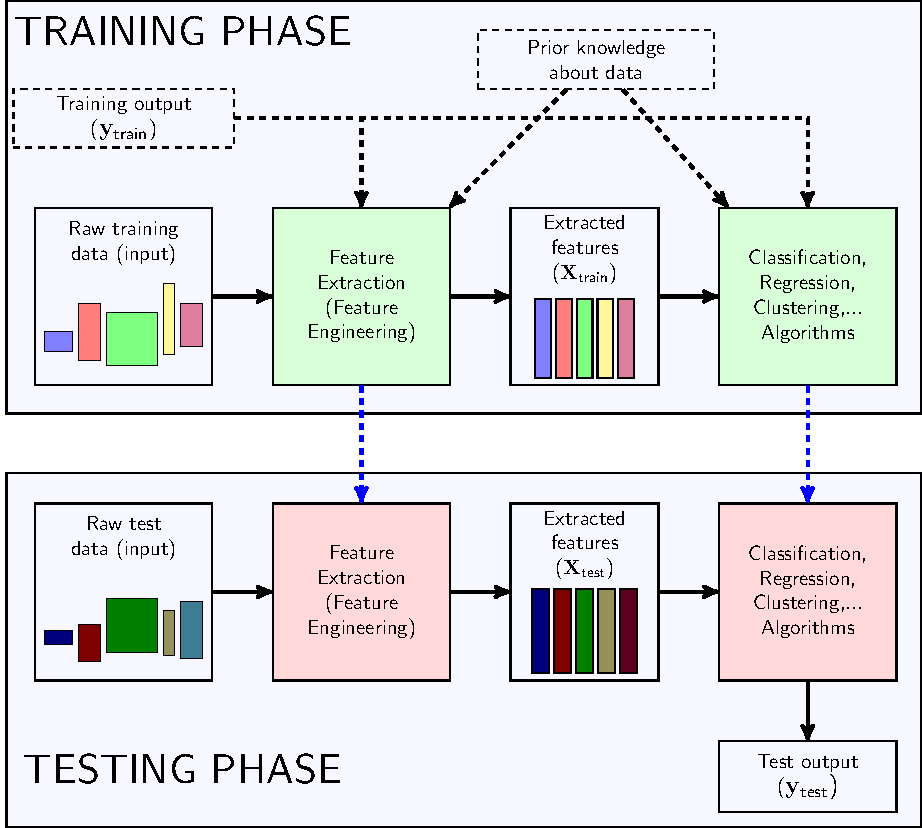
\includegraphics[width = \textwidth]{../FeatureEngineering/latex/ML_models.pdf}
   \caption{Mô hình chung cho các bài toán Machine Learning.}
   \label{fig:}
 \end{figure}
 
Có hai phases lớn là Training phase và Testing phase. Xin nhắc lại là với các bài toán Supervised learning, ta có các cặp dữ liệu (\textit{input, output}), với các bài toán Unsupervised learing, ta chỉ có \textit{input} mà thôi. 
  
 
\subsection{TRAINING PHASE }
Có hai khối có nền màu xanh lục chúng ta cần phải thiết kế:  
 
 
\subsubsection{Feature Extractor }
\textbf{ĐẦU RA} 
 
Tôi xin đề cập đầu ra của khối này trước vì mục đích của Feature Engineering là tạo ra một Feature Extractor biến dữ liệu thô ban đầu thành dữ liệu phù hợp với từng mục đích khác nhau.  
 
\textbf{ĐẦU VÀO} 
\begin{itemize}
    \item \textbf{\textit{raw training input}}. Raw input là tất cả các thông tin ta biết về dữ liệu. Ví dụ: với ảnh thì là giá trị của từng pixel; với văn bản thì là từng từ, từng câu; với file âm thanh thì nó là một đoạn tín hiệu; với cơ sở dữ liệu \href{http://machinelearningcoban.com/2017/01/08/knn/#bo-co-so-du-lieu-iris-iris-flower-dataset}{Iris} thì nó là độ dài các cánh hoa và đài hoa, ... Dữ liệu thô này thường không ở dạng vector, không có số chiều như nhau. Thậm chí có thể có số chiều như nhau nhưng số chiều quá lớn, như một bức ảnh màu 1000 pixel x 1000 pixel thì số \textit{elements} đã là $3 \times 10^6$ (3 vì ảnh màu thường có 3 channels: Red, Green, Blue). Đây là một con số quá lớn, không lợi cho lưu trữ và tính toán.  

    \item \textbf{(optional) \textit{output} của \textit{training set}}. Trong các bài toán Unsupervised learning, ta không biết \textit{output} nên hiển nhiên sẽ không có đầu vào này. Trong các bài toán Supervised learning, có khi dữ liệu này cũng không được sử dụng. Ví dụ: nếu \textit{raw input} đã có cùng số chiều rồi nhưng số chiều quá lớn,  ta muốn giảm số chiều của nó thì cách đơn giản nhất là \textit{chiếu} vector đó xuống một không gian có số chiều nhỏ hơn bằng cách lấy một ma trận ngẫu nhiên nhân với nó. Ma trận này thường là ma trận \textit{béo} (số hàng ít hơn số cột, tiếng Anh - fat matrices) để đảm bảo số chiều thu được nhỏ hơn số chiều ban đầu. Việc làm này mặc dù làm mất đi thông tin, trong nhiều trường hợp vẫn mang lại hiệu quả vì đã giảm được lượng tính toán ở phần sau. Đôi khi \textit{ma trận chiếu} không phải là ngẫu nhiên mà có thể được \textit{học} dựa trên toàn bộ \textit{raw input}, ta sẽ có bài toán tìm ma trận chiếu để lượng thông tin mất đi là ít nhất. Trong nhiều trường hợp, dữ liệu \textit{output} của \textit{training set} cũng được sử dụng để tạo ra Feature Extractor. Ví dụ: trong bài toán classification, ta không quan tâm nhiều đến việc mất thông tin hay không, ta chỉ quan tâm đến việc những thông tin còn lại có đặc trưng cho từng class hay không. Ví dụ, dữ liệu thô là các hình vuông và hình tam giác có màu đỏ và xanh. Trong bài toán phân loại đa giác, các output là \textit{tam giác} và \textit{vuông},  thì ta không quan tâm tới màu sắc mà chỉ quan tâm tới số cạnh của đa giác. Ngược lại, trong bài toán phân loại màu, các class là \textit{xanh} và \textit{đỏ}, ta không quan tâm tới số cạnh mà chỉ quan tâm đến màu sắc thôi.  

    \item \textbf{(optional) \textit{Prior knowledge about data}}: Đôi khi những giả thiết khác về dữ liệu cũng mang lại lợi ích. Ví dụ, trong bài toán classification, nếu ta biết dữ liệu là (gần như) \href{http://machinelearningcoban.com/2017/01/21/perceptron/#bai-toan-perceptron}{ \textit{linearly separable}} thì ta sẽ đi tìm một ma trận chiếu sao cho ở trong không gian mới, dữ liệu vẫn đảm bảo tính \textit{linearly separable}, việc này thuận tiện hơn cho phần classification vì các thuật toán linear, nhìn chung, đơn giản hơn.  
\end{itemize}
 
Sau khi \textit{học} được feature extractor thì ta cũng sẽ thu được \textit{extracted features} cho \textit{raw input data}. Những \textit{extracted features} này được dùng để huấn luyện các thuật toán Classification, Clustering, Regression,... ở phía sau. 
 
 
\subsubsection{Main Algorithms }
Khi có được \textit{extracted features} rồi, chúng ta sử dụng những thông tin này cùng với (optional) \textit{training output} và (optional) \textit{prior knowledge} để tạo ra các mô hình phù hợp, điều mà chúng ta đã làm ở những bài trước.  
 
\textbf{Chú ý:} Trong một số thuật toán cao cấp hơn, việc \textit{huấn luyện} feature extractor và main algorithm được thực hiện cùng lúc với nhau chứ không phải từng bước như trên.  
 
\textbf{Một điểm rất quan trọng: khi xây dựng bộ \textit{feature extractor} và \textit{main algorithms}, chúng ta không được sử dụng bất kỳ thông tin nào trong tập \textit{test data}. Ta phải giả sử rằng những thông tin trong \textit{test data} chưa được nhìn thấy bao giờ. Nếu sử dụng thêm thông tin về \textit{test data} thì rõ ràng ta đã \textit{ăn gian}! Tôi từng đánh giá các bài báo khoa học quốc tế, rất nhiều tác giả xây dựng mô hình dùng cả dữ liệu \textit{test data}, sau đó lại dùng chính mô hình đó để kiểm tra trên \textit{test data} đó. Việc \textit{ăn gian} này là lỗi rất nặng và hiển nhiên những bài báo đó bị từ chối (reject).} 
 
 
\subsection{TESTING PHASE }
Bước này đơn giản hơn nhiều. Với \textit{raw input} mới, ta sử dụng feature extractor đã tạo được ở trên (tất nhiên không được sử dụng \textit{output} của nó vì \textit{output} là cái ta đang đi tìm) để tạo ra feature vector tương ứng. Feature vector được đưa vào \textit{main algorithm} đã được học ở training phase để dự đoán \textit{output}.  
 
 
\section{Một số ví dụ về Feature Engineering}
 
\subsection{Trực tiếp lấy raw data }
Với bài toán phân loại chữ số viết tay trong bộ cơ sở dữ liệu \href{http://machinelearningcoban.com/2017/01/04/kmeans2/#bo-co-so-du-lieu-mnist}{MNIST}, mỗi bức ảnh có số chiều là 28 pixel x 28 pixel (tất nhiên việc \textit{crop} và chỉnh sửa mỗi bức ảnh đã được thực hiện từ trước rồi, đó đã là một phần của feature engineering rồi). Một cách đơn giản thường được dùng là \textit{kéo dài} ma trận 28x28 này để được 1 vector có số chiều 784. Trong cách này, các cột (hoặc hàng) của ma trận ảnh được đặt chồng lên (hoặc cạnh nhau) để được 1 vector dài. Vector dài này được trực tiếp sử dụng làm feature đưa vào các bộ classifier/clustering/regression/... Lúc này, giá trị của mỗi pixel ảnh được coi là một feature.  
 
Rõ ràng việc làm đơn giản này đã làm mất thông tin về \textit{không gian} (spatial information) giữa các điểm ảnh, tuy nhiên, trong nhiều trường hợp, nó vẫn mang lại kết quả khả quan.  
 
\subsection{Feature selection }
Giả sử rằng các điểm dữ liệu có số features khác nhau (do kích thước dữ liệu khác nhau hay do một số feature mà điểm dữ liệu này có nhưng điểm dữ liệu kia lại không thu thập được), và số lượng features là cực lớn. Chúng ta cần \textit{chọn} ra một số lượng nhỏ hơn các feature phù hợp với bài toán. \textit{Chọn thế nào} và \textit{thế nào là phù hợp} lại là một bài toán khác, tôi sẽ không bàn thêm ở đây. 
 
 
\subsection{Dimensionality reduction }
Một phương pháp nữa tôi đã đề cập đó là làm giảm số chiều của dữ liệu để giảm bộ nhớ và khối lượng tính toán. Việc giảm số chiều này có thể được thực hiện bằng nhiều cách, trong đó \textit{random projection} là cách đơn giản nhất. Tức chọn một \textit{ma trận chiếu} (projection matrix) ngẫu nhiên (ma trận béo) rồi nhân nó với từng điểm dữ liệu (giả sử dữ liệu ở dạng vector cột) để được các vector có số chiều thấp hơn. Lúc này, có thể ta không có tên gọi cho mỗi feature nữa vì các feature ở vector ban đầu đã được trộn lẫn với nhau theo một tỉ lệ nào đó rồi lưu và vector mới này. Mỗi thành phần của vector mới này được coi là một feature (không tên).  
 
Việc chọn một ma trận chiếu ngẫu nhiên đôi khi mang lại kết quả tệ không mong muốn vì thông tin bị mất đi quá nhiều. Một phương pháp được sử dụng nhiều để hạn chế lượng thông tin mất đi có tên là \href{https://en.wikipedia.org/wiki/Principal_component_analysis}{Principle Component Analysis} sẽ được tôi trình bày sau đây khoảng 1-2 tháng.  
 
\textbf{Chú ý:} Feature learning không nhất thiết phải làm giảm số chiều dữ liệu, đôi khi feature vector còn có số chiều lớn hơn raw data. Random projection cũng có thể làm được việc này nếu ma trận chiếu là một ma trận \textit{cao} (số cột ít hơn số hàng). 
 
 
\subsection{Bag-of-words }
Hẳn rất nhiều bạn đã tự đặt câu hỏi: Với một văn bản thì feature vector sẽ có dạng như thế nào? Làm sao đưa các từ, các câu, đoạn văn ở dạng \textit{text} trong các văn bản về một vector mà mỗi phần tử là một số?  
 
Có một phương pháp rất phổ biến giúp bạn trả lời những câu hỏi này. Phương pháp đó có tên là \textit{Bag of Words (BoW)} (\textit{Túi đựng Từ}). 
 
Vẫn theo thói quen, tôi bắt đầu bằng một ví dụ. Giả sử chúng ta có bài toán phân loại tin rác. Ta thấy rằng nếu một tin có chứa các từ \textit{khuyến mại, giảm giá, trúng thưởng, miễn phí, quà tặng, tri ân, ...} thì nhiều khả năng đó là một tin nhắn rác. Vậy phương pháp đơn giản nhất là \textit{đếm} xem trong tin đó có bao nhiêu từ thuộc vào các từ trên, nếu nhiều hơn 1 ngưỡng nào đó thì ta quyết định đó là tin rác. (Tất nhiên bài toán thực tế phức tạp hơn nhiều khi các từ có thể được viết dưới dạng không dấu, hoặc bị cố tình viết sai chính tả, hoặc dùng ngôn ngữ teen). Với các loại văn bản khác nhau thì lượng từ liên quan tới từng chủ đề cũng khác nhau. Từ đó có thể dựa vào số lượng các từ trong từng loại để làm các vector đặc trưng cho từng văn bản.  
 
Tôi xin lấy ví dụ cụ thể hơn về cách tạo ra vector đặc trưng cho mỗi văn bản dựa trên BoW và xin được lấy tiếng Anh làm ví dụ (nguồn \href{https://en.wikipedia.org/wiki/Bag-of-words_model}{Bag of Words wiki}. Tiếng Việt khó hơn vì một từ có thể có nhều âm tiết, tiếng Anh thì thường cứ gặp dấu cách là kết thúc một từ).  
 
Giả sử chúng ta có hai văn bản đơn giản: 
 
\begin{lstlisting}[language=Python]
(1) John likes to watch movies. Mary likes movies too. 
\end{lstlisting}
 
và  
 
\begin{lstlisting}[language=Python]
(2) John also likes to watch football games. 
\end{lstlisting}
Dựa trên hai văn bản này, ta có danh sách các từ được sử dụng, được gọi là \textit{từ điển} với 10 \textit{từ} như sau: 
 
\begin{lstlisting}[language=Python]
["John", "likes", "to", "watch", "movies", "also", "football", "games", "Mary", "too"] 
\end{lstlisting}
Với mỗi văn bản, ta sẽ tạo ra một vector đặc trưng có số chiều bằng 10, mỗi phần tử đại diện cho số từ tương ứng xuất hiện trong văn bản đó. Với hai văn bản trên, ta sẽ có hai vector đặc trưng là: 
 
\begin{lstlisting}[language=Python]
(1) [1, 2, 1, 1, 2, 0, 0, 0, 1, 1] 
(2) [1, 1, 1, 1, 0, 1, 1, 1, 0, 0] 
\end{lstlisting}
Văn bản (1) có 1 từ "John", 2 từ "likes", 0 từ "also", 0 từ "football", ... nên ta thu được vector tương ứng như trên.  
 
Có một vài điều cần lưu ý trong BoW: 
\begin{itemize}
    \item Với những ứng dụng thực tế, \textit{từ điền} có nhiều hơn 10 từ rất nhiều, có thể đến một trăm nghìn hoặc cả triệu, như vậy vector đặc trưng thu được sẽ rất \textit{dài}. Một văn bản chỉ có 1 câu, và 1 tiểu thuyết nghìn trang đều được biểu diễn bằng các vector có số chiều bằng 100 nghìn hoặc 1 triệu.

    \item Có rất nhiều từ trong từ điển không xuất hiện trong một văn bản. Như vậy các vector đặc trưng thu được thường có rất nhiều phần tử bằng 0. Các vector có nhiều phần tử bằng 0 được gọi là \textit{sparse vector} (sparse hiểu theo nghĩa là \textit{thưa thớt, rải rác}, tôi xin phép chỉ sử dụng khái niệm này bằng tiếng Anh). Để việc lưu trữ được hiệu quả hơn, ta không lưu cả vector đó mà chỉ lưu \textit{vị trí} của các phần tử khác 0 và \textit{giá trị} tương ứng. Lưu ý: nếu có hơn 50% số phần tử khác 0, việc làm này lại phản tác dụng! 

    \item Thi thoảng có những từ hiếm gặp không nằm trong từ điển, vậy ta sẽ làm gì? Một cách thường được dùng là \textit{mở rộng} vector đặc trưng thêm 1 phần tử, gọi là phẩn tử \pythoninline{<Unknown>}. Mọi từ không có trong từ điền đều được coi là \pythoninline{<Unknown>}. 

    \item Nghĩ kỹ một chút, những từ hiếm đôi khi lại mang những thông tin qua trọng nhất mà chỉ loại văn bản đó có. Đây là một nhược điểm của BoW. Có một phương pháp cải tiến khác giúp khắc phục nhược điểm này có tên là Term Frequency-Inverse Document Frequency (TF-IDF) dùng để xác định tầm quan trọng của một từ trong một văn bản dựa trên toàn bộ văn bản trong cơ sở dữ liệu (corpus). Bạn đọc muốn tìm hiểu thêm có thể xem \href{https://www.gitbook.com/book/lizrush/algorithms-for-webdevs-ebook/details}{5 Algorithms Every Web Developer Can Use and Understand, section 5.} 

    \item Nhược điểm lớn nhất của BoW là nó không mang thông tin về thứ tự của các từ. Cũng như sự liên kết giữa các câu, các đoạn văn trong văn bản. Ví dụ, ba câu sau đây: "Em yêu anh không?", "Em không yêu anh", và "Không, (nhưng) anh yêu em" khi được trích chọn đặc trưng bằng BoW sẽ cho ra ba vector giống hệt nhau, mặc dù ý nghĩa khác hẳn nhau. 
\end{itemize}
 
\textbf{Bonus:} hình dưới đay là tần suất sử dụng các từ (coi mỗi âm tiết là một từ) trong Truyện Kiều (\href{https://bitbucket.org/tiepvupsu/vietnamese/src/c6f3af6050f8ca911ed0fa209220ce3c99010075/TruyenKieu2.txt?at=master&fileviewer=file-view-default}{theo bản này}) nếu ta chỉ sử dụng 30 từ có tần suất cao nhất. : 
% <div class="imgcap"> 
% <img src ="\assets\FeatureEngineering\truyenkieu.png" align = "center" width = "400"> 
% <div class = "thecap">Hình 2: Bag of Words cho Truyện Kiều với 30 từ có tần suất cao nhất.</div> 
% </div>  
 
 
\subsection{Bag-of-Words trong Computer Vision }
Bags of Words cũng được áp dụng trong Computer Vision với cách định nghĩa \textit{words} và từ điển khác.  
 
Xét các ví dụ sau:  
 
\textbf{Ví dụ 1:} 
 
Có hai class ảnh, một class là ảnh các khu rừng, một class là ảnh các sa mạc. Phân loại một bức ảnh là rừng hay sa mạc (giả sử ta biết rằng nó thuộc một trong hai loại này) một cách trực quan nhất là dựa vào màu sắc. Màu xanh nhiều thì là rừng, màu đỏ và vàng nhiều thì là sa mạc. Vậy chúng ta có thể có một mô hình đơn giản để trích chọn đặc trưng như sau: 

\begin{itemize}
    \item Với một bức ảnh, chuẩn bị một vector $\mathbf{x}$ có số chiều bằng 3, đại diện cho 3 màu xanh ($x_1$), đỏ ($x_2$), và vàng ($x_3$).  

    \item Với mỗi điểm ảnh trong bức ảnh đó, xem nó gần với màu xanh, đỏ hay vàng nhất dựa trên giá trị của pixel đó. Nếu nó gần điểm xanh nhất, tăng $x_1$ lên 1; gần đỏ nhất, tăng $x_2$ lên 1; gần vàng nhất, tăng $x_3$ lên 1.  

    \item Sau khi xem xét tất cả các điểm ảnh, dù cho bức ảnh có kích thước thế nào, ta vẫn thu được một vector có độ dài bằng 3, mỗi phần tử thể hiện việc có bao nhiêu pixel trong bức ảnh có màu tương ứng. Vector cuối này còn được gọi là vector histogram của bức ảnh tương ứng với ba màu xanh, đỏ, vàng. Dựa vào vector này, ta có thể quyết định bức ảnh đó là ảnh rừng hay sa mạc.  
\end{itemize}
 
\textbf{Ví dụ 2:} 
 
Trên thực tế, các bài toán xử lý ảnh không đơn giản như ví dụ 1 trên đây. Mắt người thực ra nhạy với các đường nét, hình dáng hơn là màu sắc. Một cái (ảnh) cây dù không có màu vẫn là một cái (ảnh) cây! Vì vậy, xem xét giá trị từng điểm ảnh một không mang lại kết quả khả quan vì lượng thông tin bị mất quá nhiều.  
 
Có một cách khắc phục là thay vì xem xét một điểm ảnh, ta xem xét một \textit{cửa sổ} nhỏ trong ảnh (trong Computer Vision, cửa sổ này được gọi là patch) là một hình chữ nhật chứa nhiều điểm ảnh gần nhau. Cửa sổ này đủ lớn để có thể chứa được các bộ phận có thể mô tả được vật thể trong ảnh.  
 
Ví dụ với mặt người, các patch nên đủ lớn để chứa được các phần của khuôn mặt như mắt, mũi, miệng như hình dưới đây.  
 
% <div class="imgcap"> 
% <img src ="\assets\FeatureEngineering\bow_face.png" align = "center" width = "800"> 
% <div class = "thecap">Hình 3: Bag of Words cho ảnh chứa mặt người. (Nguồn <a href="http://www.robots.ox.ac.uk/~az/icvss08_az_bow.pdf"> Bag of visual words model: recognizing object categories</a>)</div> 
% </div>  
 
Tương tự thế, với ảnh là ô tô, các patch thu được có thể là bánh xe, khung xe, cửa xe, ... như hàng trên trong hình dưới đây.  
 
% <div class="imgcap"> 
% <img src ="\assets\FeatureEngineering\bow_car.png" align = "center" width = "800"> 
% <div class = "thecap">Hình 4: Bag of Words cho ảnh ô tô. (Nguồn: tôi cố gắng tìm nguồn cho hình này nhưng tất cả các tài liệu tôi tìm được đều ghi "Source: B. Leibe", tôi cũng xin được trích nguồn tương tự)</div> 
% </div>  
 
Có một câu hỏi đặt ra là, trong xử lý văn bản, hai từ được coi là như nhau nếu nó được biểu diễn bởi các ký tự giống nau. Vậy trong xử lý ảnh, hai patchés được coi là như nhau khi nào? Khi mọi pixel trong hai patches có giá trị bằng nhau sao?  
 
Câu trả lời là không. Xác suất để hai patches giống hệt nhau từng pixel là rất thấp vì có thể một phần của vật thể trong một patch bị lệch đi vài pixel so với phần đó trong patch kia; hoặc phần vật thể trong patch bị méo, hoặc có độ sáng khác nhau, mặc dù ta vẫn nhìn thấy hai patches đó \textit{rất giống nhau}. Vậy thì hai patch được coi là như nhau khi nào? Và \textit{từ điển} ở đây được định nghĩa như thế nào?  
 
Câu trả lời ngắn: hai patches là gần giống nhau nếu khoảng cách Euclid giữa hai vector tạo bởi hai patches đó gần nhau. Từ điển (codebook) sẽ có số phần tử do ta tự chọn. Số phần tử càng cao thì độ sai lệch càng ít, nhưng sẽ nặng về tính toán hơn.  
 
Câu trả lời dài: chúng ta có thể áp dụng \href{http://machinelearningcoban.com/2017/01/01/kmeans/}{K-means clustering}. Với rất nhiều patches thu được, giả sử ta muốn xây dựng một \textit{codebook} với chỉ khoảng 1000 \textit{words}. Vậy thì ta cho $k = 1000$ rồi thực hiện K-means clustering trên toàn bộ số patches thu được (từ tập training). Sau khi thực hiện K-means clustering, ta thu được 1000 clusters và 1000 centers tương ứng. Mỗi centers này được coi là một \textit{words}, và tất cả những điểm rơi vào cùng một cluster được coi là cùng một bag. Với ảnh trong tập test data, ta cũng lấy các patches rồi xem chúng rơi vào những bags nào. Từ đó suy ra vector đặc trưng cho mỗi bức ảnh. Chú ý rằng với $k = 1000$, mỗi bức ảnh sẽ được \textit{mô tả} bởi một vector có số chiều 1000, tức là mỗi điểm dữ liệu bây giờ đã có số chiều bằng nhau, mặc dù ảnh thô đầu vào có thể có kích thước khác nhau. 
 
\subsection{Feature Scaling and Normalization}
(Tham khảo \href{https://en.wikipedia.org/wiki/Feature_scaling}{Feature Scaling wiki}). 
 
Các điểm dữ liệu đôi khi được đo đạc với những đơn vị khác nhau, m và feet chẳng hạn. Hoặc có hai thành phần (của vector dữ liệu) chênh lệch nhau quá lớn, một thành phần có khoảng giá trị từ 0 đến 1000, thành phần kia chỉ có khoảng giá trị từ 0 đến 1 chẳng hạn. Lúc này, chúng ta cần chuẩn hóa dữ liệu trước khi thực hiện các bước tiếp theo.  
 
\textbf{Chú ý:} việc chuẩn hóa này chỉ được thực hiện khi vector dữ liệu đã có cùng chiều. 
 
Một vài phương pháp chuẩn hóa thường dùng: 
 
\subsubsection{Rescaling }
Phương pháp đơn giản nhất là đưa tất cả các thành phần về cùng một khoảng, $[0, 1]$ hoặc $[-1, 1]$ chẳng hạn, tùy thuộc vào ứng dụng. Nếu muốn đưa một thành phần (feature) về khoảng $[0, 1]$, công thức sẽ là:  
\begin{equation*} 
x' = \frac{x - \min(x)}{\max(x) - \min(x)} 
\end{equation*} 
trong đó $x$ là giá trị ban đầu, $x'$ là giá trị sau khi chuẩn hóa. $\min(x), \max(x)$ được tính trên toàn bộ dữ liệu training data ở cùng một thành phần. Việc này được thực hiện trên từng thành phần của vector dữ liệu $\mathbf{x}$.  
 
 
\subsubsection{Standardization }
Một phương pháp nữa cũng hay được sử dụng là giả sử mỗi thành phần đều có phân phối chuẩn với kỳ vọng là 0 và phương sai là 1. Khi đó, công thức chuẩn hóa sẽ là:  
\begin{equation*} 
x' = \frac{x - \bar{x}}{\sigma} 
\end{equation*} 
với $\bar{x}, \sigma$ lần lượt là kỳ vọng và phương sai (standard deviation) của thành phần đó trên toàn bộ training data.  
 
\subsubsection{Scaling to unit length }
Một lựa chọn khác nữa cũng được sử dụng rộng rãi là chuẩn hóa các thành phần của mỗi vector dữ liệu sao cho toàn bộ vector có độ lớn (Ecluid, tức \href{http://machinelearningcoban.com/math/#norm2}{norm 2}) bằng 1. Việc này có thể được thực hiện bằng: 
\begin{equation*} 
\mathbf{x}' = \frac{\mathbf{x}}{\|\mathbf{x}\|_2} 
\end{equation*} 
 
 
\section{Thảo luận}
Xem ra thế giới Machine Learning rất rộng lớn và có rất nhiều thứ chúng ta cần làm. Và 
vẫn có khá nhiều thứ tôi có thể viết được. Tuy nhiên, blog này sẽ không tập trung nhiều vào Feature Learning, mặc dù sẽ có một vài bài nói về Dimensionality Reduction. Tôi sẽ sử dụng các bộ dữ liệu có sẵn, và đã qua bước Feature Learning.  
 
 
\section{Tài liệu tham khảo }
[1] \href{https://en.wikipedia.org/wiki/Feature_engineering}{Feature Enginieering - wiki} 

[2] \href{https://en.wikipedia.org/wiki/Feature_scaling}{Feature Scaling wiki} 

[3] Csurka, Gabriella, et al. "\href{https://people.eecs.berkeley.edu/~efros/courses/AP06/Papers/csurka-eccv-04.pdf}{Visual categorization with bags of keypoints.}" Workshop on statistical learning in computer vision, ECCV. Vol. 1. No. 1-22. 2004.  

[4] \href{https://en.wikipedia.org/wiki/Bag-of-words_model}{Bag of Words model - wiki} 

[5] \href{https://www.kaggle.com/c/word2vec-nlp-tutorial/details/part-1-for-beginners-bag-of-words}{Bag of Words Meets Bags of Popcorn} 
 

%!TEX root = book.tex
\chapter{Binary Classifiers cho các bài toán Classification}
 
Cho tới bây giờ, ngoài \textit{thuật toán lười} \href{http://machinelearningcoban.com/2017/01/08/knn/}{K-nearest neighbors}, tôi đã giới thiệu với bạn đọc hai thuật toán cho các bài toán Classification: \href{http://machinelearningcoban.com/2017/01/21/perceptron/}{Perceptron Learning Algorithm} và \href{http://machinelearningcoban.com/2017/01/27/logisticregression/}{Logistic Regression}. Hai thuật toán này được xếp vào loại Binary Classifiers vì chúng được xây dựng dựa trên ý tưởng về các bài toán classification với chỉ hai classes. Trong bài viết này, tôi sẽ cùng các bạn làm một vài ví dụ nhỏ về ứng dụng đơn giản (nhưng thú vị) của các binary classifiers, và cách mở rộng chúng để áp dụng cho các bài toán với nhiều classes (multi-class classification problems).  
 
 
Vì Logistic Regression chỉ yêu cầu các classes là \href{http://machinelearningcoban.com/2017/01/21/perceptron/#bai-toan-perceptron}{\textit{nearly linearly separable}} (tức có thể có vài điểm làm phá vỡ tính linear separability), tôi sẽ sử dụng Logistic Regression để đại diện cho các binary classifiers. \textit{Chú ý rằng, có rất nhiều các thuật toán cho binary classification nữa mà tôi chưa giới thiệu. Tạm thời, với những gì đã viết, tôi chỉ sử dụng Logistic Regression cho các ví dụ với code mẫu. Các kỹ thuật trong bài viết này hoàn toàn có thể áp dụng cho các binary classifiers khác.} 
 
  
 
 
 
\section{Bài toán phân biệt giới tính dựa trên ảnh khuôn mặt }
Chúng ta cùng bắt đầu với bài toán phân biệt giới tính dựa trên ảnh khuôn mặt. Về ảnh khuôn mặt, bộ cơ sở dữ liệu \href{http://www2.ece.ohio-state.edu/~aleix/ARdatabase.html}{AR Face Database} được sử dụng rộng rãi.  
 
Bộ cơ sở dữ liệu này bao gồm hơn 4000 ảnh màu tương ứng với khuôn mặt của 126 người (70 nam, 56 nữ). Với mỗi người, 26 bức ảnh được chụp ở các điều kiện ánh sáng khác nhau, sắc thái biểu cảm khuôn mặt khác nhau, và bị che mắt (bởi kính râm) hoặc miệng (bởi khăn); và được chụp tại hai thời điểm khác nhau cách nhau 2 tuần.  
 
Để cho đơn giản, tôi sử dụng bộ cơ sử AR Face thu gọn (có thể tìm thấy trong cùng trang web phía trên, mục \textit{Other (relevant) downloads}). Bộ cơ sở dữ liệu thu gọn này bao gồm 2600 bức ảnh từ 50 nam và 50 nữ. Hơn nữa, các khuôn mặt cũng đã được xác định chính xác và được \textit{cropped} với kích thước 165 x 120 (pixel) bằng phương pháp được mô tả trong bài báo \href{http://lectures.molgen.mpg.de/networkanalysis13/PCAversusLDA_eigenfaces.pdf}{PCA veus LDA}. Tôi xin bỏ qua phần xử lý này và trực tiếp sử dụng ảnh đã cropped như một số ví dụ dưới đây: 
 
% <div class="imgcap"> 
% <img src ="\assets\LogReg2\ARgender.png" align = "center" width = "800"> 
% <div class = "thecap">Hình 1: Các ví dụ mẫu trong AR Face database thu gọn.</div> 
% </div>  
 
\textbf{Lưu ý:} 
\begin{itemize}
    \item \textit{Vì lý do bản quyền, tôi không được phép chia sẻ với các bạn bộ dữ liệu này. Các bạn muốn sở hữu có thể liên lạc với tác giả như hướng dẫn ở trong website \href{http://www2.ece.ohio-state.edu/~aleix/ARdatabase.html}{AR Face Database}. Một khi các bạn đã có tài khoản để download, tôi mong các bạn tôn trọng tác giả và không chia sẻ trực tiếp với bạn bè.} 

    \item \textit{Có một cách đơn giản và nhanh hơn để lấy được các feature vector (sau bước \href{http://machinelearningcoban.com/general/2017/02/06/featureengineering/}{Feature Engineering})  của cơ sở dữ liệu này mà không cần liên lạc với tác giả. Các bạn có thể tìm  \href{https://www.umiacs.umd.edu/~zhuolin/projectlcksvd.html}{tại đây}, phần \textbf{Downloads}, mục \textbf{Random face features for AR database}.} 
\end{itemize}
 
Mỗi bức ảnh trong AR Face thu gọn được đặt tên dưới dạng \pythoninline{G-xxx-yy.bmp} Trong đó: \pythoninline{G} nhận một trong hai giá trị \pythoninline{M} (man) hoặc \pythoninline{W} (woman); \pythoninline{xxx} là id của người, nhận gía trị từ \pythoninline{001} đến \pythoninline{050}; \pythoninline{yy} là điều kiện chụp, nhận giá trị từ \pythoninline{01} đến \pythoninline{26}, trong đó các điều kiện có số thứ tự từ \pythoninline{01} đến \pythoninline{07} và từ \pythoninline{14} đến \pythoninline{20} là các khuôn mặt không bị che bởi kính hoặc khăn. Tôi tạm gọi mỗi \textit{điều kiện} này là một \textit{view}. 
 
Để làm ví dụ cho thuật toán Logistic Regression, tôi lấy ảnh của 25 nam và 25 nữ đầu tiên làm tập training set; 25 nam và 25 nữ còn lại làm test set. Với mỗi người, tôi chỉ lấy các khuôn mặt không bị che bởi kính và khăn. 
 
\textbf{Feature Extraction}: vì mỗi bức ảnh có kích thước \pythoninline{3x165x120} (số channels \pythoninline{3}, chiều cao \pythoninline{165}, chiều rộng \pythoninline{120}) là một số khá lớn nên ta sẽ làm thực hiện Feature Extraction bằng hai bước đơn giản sau (\textit{bạn đọc được khuyến khích đọc bài \href{http://machinelearningcoban.com/general/2017/02/06/featureengineering/}{Giới thiệu về Feature Engineering}}):  
 
\begin{itemize}
    \item Chuyển ảnh màu về ảnh xám theo công thức \pythoninline{Y' = 0.299 R + 0.587 G + 0.114 B } (Xem thêm tại \href{https://en.wikipedia.org/wiki/Grayscale#Luma_coding_in_video_systems}{Grayscale - wiki}).  

    \item \textit{Kéo dài} ảnh xám thu được thành 1 vector hàng có số chiều \pythoninline{165x120}, sau đó sử dụng một \textit{random projection matrix} để giảm số chiều về \pythoninline{500}. Bạn đọc có thể thay giá trị này bằng các số khác nhỏ hơn \pythoninline{1000}.  
\end{itemize}
 
Chúng ta có thể bắt đầu làm việc với Python ngay bây giờ. Tôi sẽ sử dụng hàm \href{http://scikit-learn.org/stable/modules/generated/sklearn.linear_model.LogisticRegression.html}{sklearn.linear\_model.LogisticRegression} trong thư viện \pythoninline{sklearn} cho các ví dụ trong bài này. Nếu không muốn đọc phần này, bạn có thể lấy \href{http://machinelearningcoban.com/assets/LogRegs/ARgender.py}{source code ở dây}.  
 
\textbf{Chú ý:} Hàm \href{http://scikit-learn.org/stable/modules/generated/sklearn.linear_model.LogisticRegression.html}{sklearn.linear\_model.LogisticRegression} nhận dữ liệu ở dạng vector hàng.  
 
 
\subsection{Làm việc với Python}
 
Khai báo thư viện 
 
\begin{lstlisting}[language=Python]
import numpy as np  
from sklearn import linear_model           # for logistic regression 
from sklearn.metrics import accuracy_score # for evaluation 
from scipy import misc                     # for loading image 
np.random.seed(1)                          # for fixing random values 
\end{lstlisting}
 
 
Phân chia training set và test set, lựa chọn các \textit{views}. 
 
\begin{lstlisting}[language=Python]
path = '../data/AR/' # path to the database  
train_ids = np.arange(1, 26) 
test_ids = np.arange(26, 50) 
view_ids = np.hstack((np.arange(1, 8), np.arange(14, 21))) 
\end{lstlisting}
 
Tạo \textit{random projection matrix}.  
 
 
\begin{lstlisting}[language=Python]
D = 165*120 # original dimension  
d = 500 # new dimension  
 
# generate the projection matrix  
ProjectionMatrix = np.random.randn(D, d)  
\end{lstlisting}
 
Xây dựng danh sách các tên files. 
 
\begin{lstlisting}[language=Python]
def build_list_fn(pre, img_ids, view_ids): 
    """ 
    INPUT: 
        pre = 'M-' or 'W-' 
        img_ids: indexes of images 
        view_ids: indexes of views 
    OUTPUT: 
        a list of filenames  
    """ 
    list_fn = [] 
    for im_id in img_ids: 
        for v_id in view_ids: 
            fn = path + pre + str(im_id).zfill(3) + '-' + \ 
                str(v_id).zfill(2) + '.bmp' 
            list_fn.append(fn) 
    return list_fn  
\end{lstlisting}
 
\textbf{Feature Extraction:} Xây dựng dữ liệu cho training set và test set. 
 
\begin{lstlisting}[language=Python]
def rgb2gray(rgb): 
#     Y' = 0.299 R + 0.587 G + 0.114 B  
    return rgb[:,:,0]*.299 + rgb[:, :, 1]*.587 + rgb[:, :, 2]*.114 
 
# feature extraction  
def vectorize_img(filename):     
    # load image  
    rgb = misc.imread(filename) 
    # convert to gray scale  
    gray = rgb2gray(rgb) 
    # vectorization each row is a data point  
    im_vec = gray.reshape(1, D) 
    return im_vec  
 
def build_data_matrix(img_ids, view_ids): 
    total_imgs = img_ids.shape[0]*view_ids.shape[0]*2  
         
    X_full = np.zeros((total_imgs, D)) 
    y = np.hstack((np.zeros((total_imgs/2, )), np.ones((total_imgs/2, )))) 
     
    list_fn_m = build_list_fn('M-', img_ids, view_ids) 
    list_fn_w = build_list_fn('W-', img_ids, view_ids) 
    list_fn = list_fn_m + list_fn_w  
     
    for i in range(len(list_fn)): 
        X_full[i, :] = vectorize_img(list_fn[i]) 
 
    X = np.dot(X_full, ProjectionMatrix) 
    return (X, y) 
 
(X_train_full, y_train) = build_data_matrix(train_ids, view_ids) 
x_mean = X_train_full.mean(axis = 0) 
x_var  = X_train_full.var(axis = 0) 
 
def feature_extraction(X): 
    return (X - x_mean)/x_var      
 
X_train = feature_extraction(X_train_full) 
X_train_full = None ## free this variable  
 
(X_test_full, y_test) = build_data_matrix(test_ids, view_ids) 
X_test = feature_extraction(X_test_full) 
X_test_full = None  
\end{lstlisting}
 
\textbf{Chú ý:} Trong đoạn code trên tôi có sử dụng phương pháp chuẩn hóa dữ liệu \href{http://machinelearningcoban.com/general/2017/02/06/featureengineering/#standardization}{Standardization}. Trong đó \pythoninline{x_mean} và \pythoninline{x_var} lần lượt là vector kỳ vọng và phương sai của toàn bộ dữ liệu training. \pythoninline{X_train_full}, \pythoninline{X_test_full} là các ma trận dữ liệu đã được giảm số chiều nhưng chưa được chuẩn hóa. Hàm \pythoninline{feature_extraction} giúp chuẩn hóa dữ liệu dựa vào \pythoninline{x_mean} và \pythoninline{x_var} của \pythoninline{X_train_full}. 
 
Đoạn code dưới đây thực hiện thuật toán Logistic Regression, dự đoán output của test data và đánh giá kết quả. Một chú ý nhỏ, hàm Logistic Regression trong thư viện sklearn có nhiều biến thể khác nhau. Để sử dụng thuật toán Logistic Regression \textit{thuần} mà tôi đã giới thiệu trong bài \href{http://machinelearningcoban.com/2017/01/27/logisticregression/}{Logistic Regression}, chúng ta cần đặt giá trị cho \pythoninline{C} là một số lớn (để nghịch đảo của nó gần với 0. Tạm thời các bạn chưa cần quan tâm tới điều này, chỉ cần chọn \pythoninline{C} lớn là được). 
 
 
\begin{lstlisting}[language=Python]
logreg = linear_model.LogisticRegression(C=1e5) # just a big number  
logreg.fit(X_train, y_train) 
 
y_pred = logreg.predict(X_test) 
print "Accuracy: %.2f %%" %(100*accuracy_score(y_test, y_pred)) 
\end{lstlisting}
 
    Accuracy: 90.33 % 
 
90.33%, tức là cứ 10 bức ảnh trong test set thì có trung bình hơn 9 bức được nhận dạng đúng. Không tệ, nhất là khi chúng ta vẫn chưa phải làm gì nhiều! 
 
Để xác định \textit{nhãn} của một ảnh, đầu ra của hàm \href{http://machinelearningcoban.com/2017/01/27/logisticregression/#sigmoid-function}{sigmoid} được so sánh với 0.5. Nếu giá trị đó lớn hơn 0.5, ta kết luận đó là ảnh của nam, ngược lại, đó là ảnh của nữ. Để xem giá trị sau hàm sigmoid (tức xác suất để ảnh đó là nam), chúng ta sử dụng hàm \pythoninline{predict_proba} như sau: 
 
\begin{lstlisting}[language=Python]
def feature_extraction_fn(fn): 
    """ 
    extract feature from filename 
    """ 
    # vectorize 
    im = vectorize_img(fn) 
    # project 
    im1 = np.dot(im, ProjectionMatrix) 
    # standardization  
    return feature_extraction(im1) 
 
fn1 = path + 'M-036-18.bmp' 
fn2 = path + 'W-045-01.bmp' 
fn3 = path + 'M-048-01.bmp' 
fn4 = path + 'W-027-02.bmp' 
 
x1 = feature_extraction_fn(fn1) 
p1 = logreg.predict_proba(x1) 
print(p1) 
 
x2 = feature_extraction_fn(fn2) 
p2 = logreg.predict_proba(x2) 
print(p2) 
 
x3 = feature_extraction_fn(fn3) 
p3 = logreg.predict_proba(x3) 
print(p3) 
 
x4 = feature_extraction_fn(fn4) 
p4 = logreg.predict_proba(x4) 
print(p4) 
\end{lstlisting}
 
    [[ 0.87940218  0.12059782]] 
    [[ 0.0172217  0.9827783]] 
    [[ 0.30458761  0.69541239]] 
    [[ 0.83989242  0.16010758]] 
 
Kết quả thu được là xác suất để bức ảnh đó là ảnh của nam (cột thứ nhất) và của nữ (cột thứ hai). Dưới đây là hình minh họa: 
 
% <div class="imgcap"> 
% <img src ="\assets\LogReg2\ARgenderResult.png" align = "center" width = "800"> 
% <div class = "thecap">Hình 2: Ví dụ về kết quả tìm được bằng Logistic Regression</div> 
% </div>  
 
Hàng trên gồm các hình được phân loại đúng, hàng dưới gồm các hình bị phân loại sai. Có một vài nhận xét về hàng dưới. Từ hai bức ảnh hàng dưới, chúng ta có thể đoán rằng Logistic Regression quan tâm đến tóc phía sau gáy nhiều hơn là râu! Việc thuật toán dựa trên những đặc trưng nào của mỗi class phụ thuộc rất nhiều vào training data. Nếu trong training data, hầu hết nam không có râu và hầu hết nữ có tóc dài thì kết quả này là có thể lý giải được.  
 
\textbf{Trong Machine Learning, thuật toán là quan trọng, nhưng thuật toán tốt mà dữ liệu không tốt thì sẽ dẫn đến những tác dụng ngược!} 
 
(Source code cho ví dụ này có thể tìm thấy \href{http://machinelearningcoban.com/assets/LogRegs/ARgender.py}{ở dây}.) 
 
\section{Bài toán phân biệt hai chữ số viết tay }
Chúng ta cùng sang ví dụ thứ hai về phân biệt hai chữ số trong \href{http://machinelearningcoban.com/2017/01/04/kmeans2/#bo-co-so-du-lieu-mnist}{bộ cơ sở dữ liệu MNIST}. Cụ thể, tôi sẽ làm việc với hai chữ số 0 và 1. Bạn đọc hoàn toàn có thể thử với các chữ số khác bằng cách thay đổi một dòng lệnh. Khác với AR Face, bộ dữ liệu này có thể dễ dàng được download về từ \href{http://yann.lecun.com/exdb/mnist/}{trang chủ} của nó. 
 
Chúng ta có thể bắt tay vào làm luôn.  
 
Khai báo thư viện: 
 
\begin{lstlisting}[language=Python]
# %reset 
import numpy as np  
from mnist import MNIST 
import matplotlib.pyplot as plt 
from sklearn import linear_model 
from sklearn.metrics import accuracy_score 
from display_network import * 
\end{lstlisting}
 
Load toàn bộ dữ liệu: 
 
\begin{lstlisting}[language=Python]
mntrain = MNIST('../MNIST/') 
mntrain.load_training() 
Xtrain_all = np.asarray(mntrain.train_images) 
ytrain_all = np.array(mntrain.train_labels.tolist()) 
 
mntest = MNIST('../MNIST/') 
mntest.load_testing() 
Xtest_all = np.asarray(mntest.test_images) 
ytest_all = np.array(mntest.test_labels.tolist()) 
\end{lstlisting}
 
Sau bưóc này, toàn bộ dữ liệu training data và test data được lưu ở hai ma trận \pythoninline{X_train_all} và \pythoninline{X_test_all}, mỗi hàng của các ma trận này chứa một điểm dữ liệu, tức một bức ảnh đã được \textit{vector hóa}.  
 
Để lấy các hàng tương ứng với chữ số 0 và chữ số 1, ta khai báo biến sau: 
 
\begin{lstlisting}[language=Python]
cls = [[0], [1]] 
\end{lstlisting}
 
Nếu bạn muốn thử với cặp \pythoninline{3} và \pythoninline{4}, chỉ cần thay dòng này bằng \pythoninline{cls = [[3], [4]]}. Nếu bạn muốn phân loại \pythoninline{(4, 7)} và \pythoninline{(5, 6)}, chỉ cần thay dòng này bằng \pythoninline{cls = [[4, 7], [5, 6]]}. Các cặp bất kỳ khác đều có thể thực hiện bằng cách thay chỉ một dòng này.  
 
Đoạn code dưới đây thực hiện việc \textit{extract} toàn bộ dữ liệu cho các chữ số \pythoninline{0} và \pythoninline{1} trong tập training data và test data.  
 
\begin{lstlisting}[language=Python]
def extract_data(X, y, classes): 
    """ 
    X: numpy array, matrix of size (N, d), d is data dim 
    y: numpy array, size (N, ) 
    cls: two lists of labels. For example:  
        cls = [[1, 4, 7], [5, 6, 8]] 
    return: 
        X: extracted data 
        y: extracted label  
            (0 and 1, corresponding to two lists in cls) 
    """ 
    y_res_id = np.array([]) 
    for i in cls[0]: 
        y_res_id = np.hstack((y_res_id, np.where(y == i)[0])) 
    n0 = len(y_res_id) 
 
    for i in cls[1]: 
        y_res_id = np.hstack((y_res_id, np.where(y == i)[0])) 
    n1 = len(y_res_id) - n0  
 
    y_res_id = y_res_id.astype(int) 
    X_res = X[y_res_id, :]/255.0 
    y_res = np.asarray([0]*n0 + [1]*n1) 
    return (X_res, y_res) 
 
 
# extract data for training  
(X_train, y_train) = extract_data(Xtrain_all, ytrain_all, cls) 
 
# extract data for test  
(X_test, y_test) = extract_data(Xtest_all, ytest_all, cls) 
\end{lstlisting}
 
Vì mỗi điểm dữ liệu có số phần tử là 784 (28x28), là một số khá nhỏ, nên ta không cần thêm bước giảm số chiều dữ liệu nữa. Tuy nhiên, tôi có thực hiện thêm một bước chuẩn hóa để đưa dữ liệu về đoạn \pythoninline{[0, 1]} bằng cách chia toàn bộ hai ma trận dữ liệu cho \pythoninline{255.0}. 
 
Tới đây ta có thể \textit{train} mô hình Logistic Regression và đánh giá mô hình này.   
 
\begin{lstlisting}[language=Python]
# train the logistic regression model  
logreg = linear_model.LogisticRegression(C=1e5) # just a big number  
logreg.fit(X_train, y_train) 
 
# predict  
y_pred = logreg.predict(X_test) 
print "Accuracy: %.2f %%" %(100*accuracy_score(y_test, y_pred.tolist())) 
\end{lstlisting}
 
    Accuracy: 99.95 % 
 
Tuyệt vời, gần như 100% được phân loại chính xác. Điều này là dễ hiểu vì hai chữ số 0 và 1 khác nhau quá nhiều. Bộ cơ sở dữ liệu này với toàn bộ 10 classes hiện nay đã được phân loại với độ chính xác trên 99.7%.  
 
Chúng ta cùng đi tìm những ảnh bị phân loại sai: 
 
\begin{lstlisting}[language=Python]
# display misclassified image(s) 
mis = np.where((y_pred - y_test) != 0)[0] 
Xmis = X_test[mis, :] 
 
plt.axis('off') 
A = display_network(Xmis.T) 
f2 = plt.imshow(A, interpolation='nearest' ) 
plt.gray() 
plt.show() 
\end{lstlisting}
 
% <div class="imgcap"> 
% <img src ="\assets\LogReg2\0.png" align = "center" width = "100"> 
% <div class = "thecap">Hình 3: Chữ số bị phân loại sai trong bài toán phân loại ảnh chữ số 0 và 1</div> 
% </div>  
 
Như vậy là chỉ có một ảnh bị phân loại sai. Ảnh này là chữ số 0 nhưng bị misclassified thành chữ số 1, có thể vì nét đậm nhất của nó rất giống với chữ số 1.  
 
Source code cho ví dụ này có thể được tìm thấy \href{http://machinelearningcoban.com/assets/LogReg2/LogReg2.ipynb}{ở đây}. 
 
 
\section{Binary Classifiers cho Multi-class Classification problems }
 
Có lẽ nhiều bạn đang đặt câu hỏi: Các ví dụ trên đây đều làm với bài toán có hai classes. Vậy nếu có nhiều hơn hai classes, ví dụ như 10 classes của MNIST, thì làm thế nào? 
 
Có nhiều thuật toán khác được xây dựng riêng cho các bài toán với nhiều classes (multi-class classification problems), tôi sẽ giới thiệu sau. Còn bây giờ, chúng ta vẫn có thể sử dụng các \textit{binary classifiers} để thực hiện công việc này, với một chút thay đổi.  
 
Có \textit{ít nhất} bốn cách để áp dụng \textit{binary classifiers} vào các bài toán multi-class classification: 
 
 
\subsection{One-vs-one}
 
Xây dựng rất nhiều bộ binary classifiers cho từng cặp classes. Bộ thứ nhất phân biệt class 1 và class 2, bộ thứ hai phân biệt class 1 và class 3, ... Khi có một dữ liệu mới vào, đưa nó vào toàn bộ các bộ binary classifiers trên. Kết quả cuối cùng có thể được xác định bằng cách xem class nào mà điểm dữ liệu đó được phân vào nhiều nhất (major voting). Hoặc với Logistic Regression thì ta có thể tính \textit{tổng các xác suất} tìm được sau mỗi bộ binary classifier.  
  
Như vậy, nếu có $C$ classes thì tổng số binary classifiers phải dùng là $\frac{n(n-1)}{2}$. Đây là một con số lớn, cách làm này không lợi về tính toán. Hơn nữa, nếu một chữ số thực ra là chữ số \pythoninline{1}, nhưng lại được đưa vào bộ phân lớp giữa các chữ số \pythoninline{5} và \pythoninline{6}, thì cả hai khả năng tìm được (là \pythoninline{5} hoặc \pythoninline{6}) đều không hợp lý! 
 
 
\subsection{Hierarchical (phân tầng)}
Các làm như \textbf{one-vs-one} sẽ mất rất nhiều thời gian training vì có quá nhiều bộ phân lớp cần được xây dựng. Một cách khác giúp \textit{tiết kiệm} số binary classifiers hơn đó là \textbf{hierarchical}. Ý tưởng như sau: 
 
Ví dụ với MNIST với 4 chữ số \pythoninline{4, 5, 6, 7}. Vì ta thấy chữ số \pythoninline{4} và \pythoninline{7} khá giống nhau, chữ số \pythoninline{5} và \pythoninline{6} khá giống nhau nên trước tiên chúng ta xây dựng bộ phân lớp \pythoninline{[4, 7] vs [5, 6]}. Sau đó xây dựng thêm hai bộ \pythoninline{4 vs  7} và \pythoninline{5 vs 6} nữa. Tổng cộng, ta cần 3 bộ binary classifiers. Chú ý rằng có nhiều cách chia khác nhau, ví dụ \pythoninline{[4, 5, 6] vs 7}, \pythoninline{[4, 5] vs 6}, rồi \pythoninline{4 vs 5}.  
 
 
Ưu điểm của phương pháp này là sử dụng ít bộ binary classifiers hơn \textbf{one-vs-one}.  
Hạn chế lớn nhất của nó là việc nếu chỉ một binary classifier cho kết quả sai thì kết quả cuối cùng chắc chắn sẽ sai. Ví dụ, nếu 1 ảnh chứa chữ số \pythoninline{5}, nhưng ngay bước đầu tiên đã bị misclassifed sang nhánh \pythoninline{[4, 7]} thì kết quả cuối cùng sẽ là \pythoninline{4} hoặc \pythoninline{7}, cả hai đều sai.  
 
 
\subsection{Binary coding}
Có một cách giảm số binary classifiers hơn nữa là \textbf{binary coding}, tức \textit{mã hóa} output của mỗi class bằng một số nhị phân. Ví dụ, nếu có 4 classes thì class thứ nhất được mã hóa là \pythoninline{00}, ba class kia được mã hóa lần lượt là \pythoninline{01, 10} và \pythoninline{11}. Với cách làm này, số bộ binary classifiers phải thực hiện chỉ là $m = \left\lceil\log_2(C)\right\rceil$ trong đó $C$ là số lượng class, $\left\lceil a \right\rceil$ là \textit{số nguyên nhỏ nhất không nhỏ hơn} $a$. Class thứ nhất sẽ đi tìm bit đầu tiên của output (đã được mã hóa nhị phân), class thứ hai sẽ đi tìm bit thứ hai, ... 
 
Cách làm này sử dụng một số lượng nhỏ nhất các bộ \textit{binary classifiers}. Nhưng nó có một hạn chế rất lớn là chỉ cần một bit bị phân loại sai sẽ dẫn đến dữ liệu bị phân loại sai. Hơn nữa, nếu số classes không phải là lũy thừa của hai, mã nhị phân nhận được có thể là một giá trị không tương ứng với class nào! 
 
 
\subsection{one-vs-rest hay one-hot coding}
Phương pháp được sử dụng nhiều nhất là \textbf{one-vs-rest} (một số tài liệu gọi là \textbf{ove-vs-all}, \textbf{one-against-rest}, hoặc \textbf{one-against-all}) . Cụ thể, nếu có $C$ classes thì ta sẽ xây dựng $C$ classifiers, mỗi classifier tương ứng với một class. Classifier thứ nhất giúp phân biệt \pythoninline{class 1} vs \pythoninline{not class 1}, tức xem một điểm có thuộc class 1 hay không, hoặc xác suất để một điểm rơi vào class 1 là bao nhiêu. Tương tự như thế, classifier thứ hai sẽ phân biệt \pythoninline{class 2} vs \pythoninline{not class 2}, ... Kết quả cuối cùng có thể được xác định bằng cách xác định class mà một điểm rơi vào với xác suất cao nhất.  
 
Phương pháp này còn được gọi là \textbf{one-hot coding} (được sử dụng nhiều nên có rất nhiều tên) vì với cách mã hóa trên, giả sử có 4 classes, class 1, 2, 3, 4 sẽ lần lượt được mã hóa dưới dạng nhị phân bởi \pythoninline{1000, 0100, 0010} hoặc \pythoninline{0001}. One-hot vì chỉ có \textit{one} bit là \textit{hot} (bằng \pythoninline{1}).  
 
Hàm Logistic Regression trong thư viện sklearn có thể được dùng trực tiếp để áp dụng vào các bài toán multi-class classification với phương pháp \textbf{one-vs-rest}. Với bài toán MNIST như nêu ở phần 2, ta có thể thêm ba dòng lệnh sau để chạy trên toàn bộ 10 classes: 
 
\begin{lstlisting}[language=Python]
logreg.fit(Xtrain_all, ytrain_all) 
y_pred = logreg.predict(Xtest_all) 
print "Accuracy: %.2f %%" %(100*accuracy_score(ytest_all, y_pred.tolist())) 
\end{lstlisting}
 
Kết quả thu được khoảng 91\% sau hơn 20 phút chạy (tùy thuộc vào máy). Đây vẫn là một kết quả quá thấp so với con số 99.7\%. Thậm chí phương pháp học máy \textit{không học gì} như \href{http://machinelearningcoban.com/2017/01/08/knn/#try-this-yourself}{K-neareast neighbors cũng đã đạt hơn 96\%} với thời gian chạy ngắn hơn một chút.  
 
Một chú ý nhỏ: phương pháp mặc định cho các bài toán multi-class của hàm này được xác định bởi biến \pythoninline{multi_class}. Có hai lựa chọn cho biến này, trong đó lựa chọn mặc định là \pythoninline{ovr} tức \textbf{one-vs-rest}, lựa chọn còn lại sẽ được tôi đề cập trong một bài gần đây. Lựa chọn thứ hai không phải cho binary classifiers nên tôi không đề cập trong bài này, có thể sau một vài bài nữa (Xem thêm \href{http://scikit-learn.org/stable/modules/generated/sklearn.linear_model.LogisticRegression.html}{\pythoninline{sklearn.linear_model.LogisticRegression}}) 
 
 
 
\section{Thảo luận }
 
\subsection{Kết hợp các phương pháp trên}
 
Nhắc lại rằng các linear binary classifiers tôi đã trình bày yêu cầu dữ liệu là \textit{linearly separable} hoặc \textit{nearly linearly separable}. Ta cũng có thể mở rộng định nghĩa này cho các bài toán multi-class. Nếu hai class bất kỳ là \textit{linearly separable} thì ta coi dữ liệu đó là \textit{linearly separable}.  
 
Thế nhưng, có những loại dữ liệu \textit{linearly separable} mà chỉ một số trong 4 phương pháp trên đây là phù hợp, hoặc có những loại dữ liệu yêu cầu phải kết hợp nhiều phương pháp mới thực hiện được. Xét ba ví dụ sau: 
 
% <div class="imgcap"> 
% <img src ="\assets\LogReg2\dist.png" align = "center" width = "800"> 
% <div class = "thecap">Hình 4: Một số ví dụ về phân phối của các classes trong bài toàn multi-class</div> 
% </div>  
 
\begin{itemize}
    \item Hình 4a): cả 4 phương pháp trên đây đều có thể áp dụng được. 

    \item Hình 4b): one-vs-rest không phù hợp vì class màu xanh lục và class \textit{rest} (hợp của xanh lam và đỏ) là không \textit{linearly separable}. Lúc này, one-vs-one hoặc hierarchical phù hợp hơn.  

    \item Hình 4c): Tương tự như trên, ba class lam, lục, đỏ thẳng hàng nên sẽ không dùng được one-vs-rét. one-vs-one vẫn làm việc vì từng đôi class một là \textit{linearly separable}. Tương tự hierarchical cũng làm việc nếu ta phân chia các nhóm một cách hợp lý. Hoặc chúng ta có thể kết hợp nhiều phương pháp. Ví dụ: dùng one-vs-rest để tìm \textit{đỏ} vs \textit{không đỏ}. Nếu một điểm dữ liệu là \textit{không đỏ}, với 3 class còn lại, chúng ta lại quay lại trường hợp Hình 4a) và có thể dùng các phương pháp khác. Nhưng khó khăn vẫn nằm ở việc phân nhóm như thế nào, liệu rằng những class nào có thể cho vào cùng một nhóm? Với những dữ liệu đơn giản, \href{http://machinelearningcoban.com/2017/01/01/kmeans/}{K-means clustering} có thể là một giải pháp! 
\end{itemize}
 
Bạn đọc có thể xem thêm ví dụ áp dụng Logistic Regression cho cơ sở dữ liệu \href{http://machinelearningcoban.com/2017/01/08/knn/#bo-co-so-du-lieu-iris-iris-flower-dataset}{Iris} trong \href{http://scikit-learn.org/stable/auto_examples/linear_model/plot_iris_logistic.html}{link này} 
 
 
 
% <div class="imgcap"> 
% <img src ="http://scikit-learn.org/stable/_images/sphx_glr_plot_iris_logistic_001.png" align = "center" width = "500"> 
% <div class = "thecap">Hình 5: Logistic Regression với Iris database. (Nguồn: <a href="http://scikit-learn.org/stable/auto_examples/linear_model/plot_iris_logistic.html">Logistic Regression 3-class Classifier</a>)</div> 
% </div>  
 
 
 
\subsection{Biểu diễn dưới dạng Neural Networks}
Lấy ví dụ với bài toán có 4 classes 1, 2, 3, 4; ta có thể biểu diễn các mô hình được đề cập trong phần 3 dưới dạng sau đây (giả sử input có số chiều là 7 và node output màu đỏ biểu diễn chung cho cả PLA, Logistic Regression và các networks với activation function khác):  
 
% <div class="imgcap"> 
% <img src ="\assets\LogReg2\binaryclassifiers.png" align = "center" width = "800"> 
% <div class = "thecap">Hình 6: Mô hình neural networks cho các phương pháp đề cập trong bài</div> 
% </div>  
 
Lúc này, thay vì chỉ có 1 node output như \href{http://machinelearningcoban.com/2017/01/27/logisticregression/#-thao-luan}{các phương pháp tôi đề cập trước đây} (Linear Regression, Perceptron Learning Algorithm, Logistic Regression), chúng ta thấy rằng các networks này đều có nhiều outputs. Và một vector trọng số $\mathbf{w}$ bây giờ đã trở thành \textit{ma trận trọng số} $\mathbf{W}$ mà mỗi cột của nó tương ứng với vector trọng số của một node output. Việc tối ưu đồng thời các binary classifiers trong mỗi network cũng được tổng quát lên nhớ các phép tính với ma trận.  
 
Lấy ví dụ với công thức cập nhật của \href{http://machinelearningcoban.com/2017/01/27/logisticregression/#cong-thuc-cap-nhat-cho-logistic-sigmoid-regression}{logistic sigmoid regression }: 
 
\begin{equation*} 
\mathbf{w} = \mathbf{w} + \eta(y_i - z_i)\mathbf{x}_i 
\end{equation*} 
 
Có thể tổng quát thành: 
\begin{equation*} 
\mathbf{W} = \mathbf{W} + \eta\mathbf{x}_i(\mathbf{y}_i - \mathbf{z}_i)^T 
\end{equation*} 
 
Với $\mathbf{W}, \mathbf{y}_i, \mathbf{z}_i$ lần lượt là ma trận trọng số, vector (cột) output \textit{thật} với toàn bộ các binary classifiers tương ứng với điểm dữ liệu $\mathbf{x}_i$, và vector output tìm được của networks tại thời điểm đang xét nếu đầu vào mỗi network là $\mathbf{x}_i$. Chú ý rằng với Logistic Regression, vector $\mathbf{y}_i$ là một binary vector, vector $\mathbf{z}_i$ gồm các phần tử nằm trong khoảng $(0, 1)$.  
 
 
\subsection{Hạn chế của one-vs-rest}
Xem xét lại phương pháp one-vs-rest theo góc nhìn xác suất, một điểm dữ liệu có thể được dự đoán thuộc vào class $1, 2, \dots, C$ với xác suất lần lượt là $p_1, p_2, \dots, p_C$. Tuy nhiên, tổng các xác suất này có thể không bằng 1! Có một phương pháp có thể làm cho nó \textit{hợp lý hơn}, tức \textit{ép} tổng các xác suất này bằng 1. Khi đó, với 1 điểm dữ liệu ta có thể nói xác suất nó rơi vào mỗi class là bao nhiêu. Phương pháp hấp dẫn này sẽ được đề cập trong bài \href{http://machinelearningcoban.com/2017/02/16/softmax/}{Softmax Regression}. Mời bạn đón đọc. 
 
 
\section{Tài liệu tham khảo}
 
 
[1] \href{https://en.wikipedia.org/wiki/Multiclass_classification}{Multiclass classification - wiki} 
 
[2] \href{http://scikit-learn.org/stable/auto_examples/linear_model/plot_iris_logistic.html}{Logistic Regression 3-class Classifier} 

%!TEX root = book.tex
\chapter{Softmax Regression}
--- 
 
 
 
Các bài toán classification thực tế thường có rất nhiều classes (multi-class), các \href{http://machinelearningcoban.com/2017/02/11/binaryclassifiers/#-binary-classifiers-cho-multi-class-classification-problems}{binary classifiers mặc dù có thể áp dụng cho các bài toán multi-class}, chúng vẫn có những hạn chế nhất định. Với binary classifiers, kỹ thuật được sử dụng nhiều nhất \href{http://machinelearningcoban.com/2017/02/11/binaryclassifiers/#one-vs-rest-hay-one-hot-coding}{\textbf{one-vs-rest}} có \href{http://machinelearningcoban.com/2017/02/11/binaryclassifiers/#han-che-cua-one-vs-rest}{một hạn chế về tổng các xác suất}. Trong post này, một phương pháp mở rộng của Logistic Regression sẽ được giới thiệu giúp khắc phục hạn chế trên. Một lần nữa, dù là Softmax \textbf{Regression}, phương pháp này được sử dụng rộng rãi như một phương pháp classification.  
 
 
  
\textbf{Một lưu ý nhỏ:} Hàm mất mát của Softmax Regression trông có vẻ khá phức tạp, nhưng nếu  kiên trì đọc đến phần phương pháp tối ưu, các bạn sẽ thấy vẻ đẹp ẩn sau sự phức tạp đó. Gradient của hàm mất mát và công thức cập nhật ma trận trọng số là rất đơn giản. (Đơn giản sau vài bước biến đổi toán học \textit{trông có vẻ} phức tạp). 
 
Nếu có điểm nào khó hiểu, bạn đọc được khuyến khích đọc lại các bài trước, trong đó quan trọng nhất là \href{http://machinelearningcoban.com/2017/01/27/logisticregression/}{Bài 10: Logistic Regression}. 
 
\section{Giới thiệu }
Tôi xin phép được bắt đầu từ mô hình \href{http://machinelearningcoban.com/2017/02/11/binaryclassifiers/#one-vs-rest-hay-one-hot-coding}{\textbf{one-vs-rest}} được trình bày trong bài trước. Output layer (màu đỏ nhạt) có thể phân tách thành hai \textit{sublayer} như hình dưới đây: 
 
% <div class="imgcap"> 
% <img src ="\assets\13_softmax\onevsrest.png" align = "center" width = "600"> 
% <div class = "thecap">Hình 1: Multi-class classification với Logistic Regression và one-vs-rest.</div> 
% </div>  
 
Dữ liệu $\mathbf{x}$ có số chiều là $(d +1)$ vì có phần tử 1 được thêm vào phía trước, thể hiện hệ số tự do trong hàm tuyến tính. Hệ số tự do $w_{0j}$ còn được gọi là bias.  
 
Giả sử số classes là $C$. Với one-vs-rest, chúng ta cần xây dựng $C$ Logistic Regression khác nhau. Các \textit{đầu ra dự đoán} được tính theo hàm sigmoid: 
\begin{equation*} 
a_i = \text{sigmoid}(z_i) = \text{sigmoid}(\mathbf{w}_i^T\mathbf{x}) 
\end{equation*} 
Trong kỹ thuật này, các phần tử $a_i, i = 1, 2, \dots, C$ được suy ra trực tiếp chỉ với $z_i$. Vì vậy, không có mối quan hệ chặt chẽ nào giữa các $a_i$, tức tổng của chúng có thể nhỏ hơn hoặc lớn hơn 1. Nếu ta có thể khai thác được mỗi quan hệ giữa các $z_i$ thì kết quả của bài toán classification có thể tốt hơn.  
 
Chú ý rằng các mô hình Linear Regression, PLA, Logistic Regression chỉ có 1 node ở output layer. Trong các trường hợp đó, tham số mô hình chỉ là 1 vector $\mathbf{w}$. Trong trường hợp output layer có nhiều hơn 1 node, tham số mô hình sẽ là tập hợp  
tham số $\mathbf{w}_i$ ứng với từng node. Lúc này, ta có \textit{ma trận trọng số} $\mathbf{W} = [\mathbf{w}_1, \mathbf{w}_2, \dots, \mathbf{w}_C]$. 
 
 
\section{Softmax function }
 
\subsection{Công thức của Softmax function}
Chúng ta cần một mô hình xác suất sao cho với mỗi input $\mathbf{x}$, $a_i$ thể hiện xác suất để input đó rơi vào class $i$. Vậy điều kiện cần là các $a_i$ phải dương và tổng của chúng bằng 1. Để có thể thỏa mãn điều kiện này, chúng ta cần \textit{nhìn vào} mọi giá trị $z_i$ và dựa trên quan hệ giữa các $z_i$ này để tính toán giá trị của $a_i$. Ngoài các điều kiện $a_i$ lớn hơn 0 và có tổng bằng 1, chúng ta sẽ thêm một điều kiện cũng rất tự nhiên nữa, đó là: giá trị $z_i = \mathbf{w}_i^T\mathbf{x}$ càng lớn thì xác suất dữ liệu rơi vào class $i$ càng cao. Điều kiện cuối này chỉ ra rằng chúng ta cần một hàm đồng biến ở đây. 
 
Chú ý rằng $z_i $ có thể nhận giá trị cả âm và dương. Một hàm số \textit{mượt} đơn giản có thể chắc chắn biến  $z_i $ thành một giá trị dương, và hơn nữa, đồng biến, là hàm $\exp(z_i) = e^{z_i}$. Điều kiện \textit{mượt} để thuận lợi hơn trong việc tính đạo hàm sau này. Điều kiện cuối cùng, tổng các $a_i$ bằng 1 có thể được đảm bảo nếu: 
 
\begin{equation*} 
a_i = \frac{\exp(z_i)}{\sum_{j=1}^C \exp(z_j)}, ~~ \forall i = 1, 2, \dots, C 
\end{equation*} 
 
Hàm số này, tính tất cả các $a_i$ dựa vào tất cả các $z_i$, thõa mãn tất cả các điều kiện đã xét: dương, tổng bằng 1, giữ được \textit{thứ tự} của $z_i$. Hàm số này được gọi là \textit{softmax function}. Chú ý rằng với cách định nghĩa này, không có xác suất $a_i$ nào tuyệt đối bằng 0 hoặc tuyệt đối bằng 1, mặc dù chúng có thể rất gần 0 hoặc 1 khi $z_i$ rất nhỏ hoặc rất lớn khi so sánh với các $z_j, j \neq i$. 
 
Lúc này, ta có thể giả sử rằng: 
 
\begin{equation*} 
P(y_k = i | \mathbf{x}_k; \mathbf{W}) = a_i 
\end{equation*} 
 
Trong đó, $P(y = i \| \mathbf{x}; \mathbf{W})$ được hiểu là xác suất để một điểm dữ liệu $\mathbf{x}$ rơi vào class thứ $i$ nếu biết tham số mô hình (ma trận trọng số) là $\mathbf{W}$.  
 
 
Hình vẽ dưới đây thể hiện mạng Softmax Regression dưới dạng neural network: 
% <div class="imgcap"> 
% <img src ="\assets\13_softmax\softmax_nn.png" align = "center" width = "800"> 
% <div class = "thecap">Hình 2: Mô hình Softmax Regression dưới dạng Neural network.</div> 
% </div>  
 
Ở phần bên phải, hàm tuyến tính $\Sigma$ và hàm softmax (activation function) được tách riêng ra để phục vụ cho mục đích minh họa. Dạng \textit{short form} ở bên phải là dạng hay được sử dụng trong các Neural Networks, lớp $\mathbf{a}$ được ngầm hiểu là bao gồm cả lớp $\mathbf{z}$. 
 
 
 
 
\subsection{Softmax function trong Python }
Dưới đây là một đoạn code viết hàm softmax. Đầu vào là một ma trận với mỗi cột là một vector $\mathbf{z}$, đầu ra cũng là một ma trận mà mỗi cột có giá trị là $\mathbf{a} = \text{softmax}(\mathbf{z})$. Các giá trị của $\mathbf{z}$ còn được gọi là \textbf{scores}. 
 
\begin{lstlisting}[language=Python]
import numpy as np  
 
def softmax(Z): 
    """ 
    Compute softmax values for each sets of scores in V. 
    each column of V is a set of score.     
    """ 
    e_Z = np.exp(Z) 
    A = e_Z / e_Z.sum(axis = 0) 
    return A 
\end{lstlisting}
 
 
\subsection{Một vài ví dụ }
 
Hình 3 dưới đây là một vài ví dụ về mối quan hệ giữa đầu vào và đầu ra của hàm softmax. Hàng trên màu xanh nhạt thể hiện các scores $z_i$ với giả sử rằng số classes là 3. Hàng dưới màu đỏ nhạt thể hiện các giá trị đầu ra $a_i$ của hàm softmax. 
 
% <div class="imgcap"> 
% <img src ="\assets\13_softmax\softmax_ex.png" align = "center" width = "600"> 
% <div class = "thecap">Hình 3: Một số ví dụ về đầu vào và đầu ra của hàm softmax.</div> 
% </div>  
 
Có một vài quan sát như sau:  

\begin{itemize}
    \item Cột 1: Nếu các $z_i$ bằng nhau, thì các $a_i$ cũng bằng nhau và bằng 1/3.  
     
    \item Cột 2: Nếu giá trị lớn nhất trong các $z_i$ là $z_1$ vẫn bằng 2, nhưng các giá trị khác thay đổi, thì mặc dù xác suất tương ứng $a_1$ vẫn là lớn nhất, nhưng nó đã thay đổi lên hơn 0.5. Đây chính là một lý do mà tên của hàm này có từ \textit{soft}. (\textit{max} vì phẩn từ lớn nhất vẫn là phần tử lớn nhất). 
     
    \item Cột 3: Khi các giá trị $z_i$ là âm thì các giá trị $a_i$ vẫn là dương và thứ tự vẫn được đảm bảo.  
     
    \item Cột 4: Nếu $z_1 = z_2$, thì $a_1 = a_2$. 
\end{itemize}
 
Bạn đọc có thể thử với các giá trị khác trực tiếp trên trình duyệt trong \href{http://neuralnetworksanddeeplearning.com/chap3.html}{link này}, kéo xuống phần Softmax.  
 
 
\subsection{Phiên bản ổn định hơn của softmax function }
 
Khi một trong các $z_i$ quá lớn, việc tính toán $\exp(z_i)$ có thể gây ra hiện tượng tràn số (overflow), ảnh hưởng lớn tới kết quả của hàm softmax. Có một cách khắc phục hiện tượng này bằng cách dựa trên quan sát sau:  
 
\begin{eqnarray*}
\frac{\exp(z_i)}{\sum_{j=1}^C \exp(z_j)} &=& \frac{\exp(-c)\exp(z_i)}{\exp(-c)\sum_{j=1}^C \exp(z_j)}\\\ 
&=& \frac{\exp(z_i-c)}{\sum_{j=1}^C \exp(z_j-c)} 
\end{eqnarray*}
với $c$ là một hằng số bất kỳ.  
 
Vậy một phương pháp đơn giản giúp khắc phục hiện tượng overflow là trừ tất cả các $z_i$ đi một giá trị đủ lớn. Trong thực nghiệm, giá trị đủ lớn này thường được chọn là $c = \max_i z_i$. Vậy chúng ta có thể sửa đoạn code cho hàm \pythoninline{softmax} phía trên bằng cách trừ mỗi cột của ma trận đầu vào \pythoninline{V} đi giá trị lớn nhất trong cột đó. Ta có phiên bản ổn định hơn là \pythoninline{softmax_stable}: 
 
\begin{lstlisting}[language=Python]
def softmax_stable(Z): 
    """ 
    Compute softmax values for each sets of scores in V. 
    each column of V is a set of score.     
    """ 
    e_Z = np.exp(Z - np.max(Z, axis = 0, keepdims = True)) 
    A = e_Z / e_Z.sum(axis = 0) 
    return A 
\end{lstlisting}
 
trong đó \pythoninline{axis = 0} nghĩa là lấy \pythoninline{max} theo cột (\pythoninline{axis = 1} sẽ lấy max theo hàng), \pythoninline{keepdims = True} để đảm bảo phép trừ giữa ma trận \pythoninline{V} và vector  thực hiện được.  
 
 
 
 
 
 
\section{Hàm mất mát và phương pháp tối ưu }
 
 
\subsection{One hot coding }
Với cách biểu diễn network như trên, mỗi output sẽ không còn là một giá trị tương ứng với mỗi class nữa mà sẽ là một vector có đúng 1 phần tử bằng 1, các phần tử còn lại bằng 0. Phần tử bằng 1 năm ở vị trí tương ứng với class đó, thể hiện rằng điểm dữ liệu đang xét rơi vào class này với xác suất bằng 1 (\textit{sự thật} là như thế, không cần dự đoán). Cách \textit{mã hóa} output này chính là \textit{one-hot coding} mà tôi đã đề cập trong bài \href{http://machinelearningcoban.com/2017/01/01/kmeans/}{K-means clustering} và \href{http://machinelearningcoban.com/2017/02/11/binaryclassifiers/#one-vs-rest-hay-one-hot-coding}{bài trước}.  
 
Khi sử dụng mô hình Softmax Regression, với mỗi đầu vào $\mathbf{x}$, ta sẽ có \textit{đầu ra dự đoán} là $\mathbf{a} = \text{softmax}(\mathbf{W}^T\mathbf{x})$. Trong khi đó, \textit{đầu ra thực sự} chúng ta có là vector $\mathbf{y}$ được biểu diễn dưới dạng one-hot coding.  
 
Hàm mất mát sẽ được xây dựng để tối thiểu sự khác nhau giữa \textit{đầu ra dự đoán} $\mathbf{a}$ và \textit{đầu ra thực sự} $\mathbf{y}$. Một lựa chọn đầu tiên ta có thể nghĩ tới là: 
 
\begin{equation*} 
J(\mathbf{W}) = \sum_{i=1}^N \|\|\mathbf{a}_i - \mathbf{y}_i\|\|_2^2 
\end{equation*} 
\textbf{Tuy nhiên đây chưa phải là một lựa chọn tốt}. Khi đánh giá sự khác nhau (hay khoảng cách) giữa hai phân bố xác suất (probability distributions), chúng ta có một đại lượng đo đếm khác hiệu quả hơn. Đại lượng đó có tên là \href{https://en.wikipedia.org/wiki/Cross_entropy}{\textbf{cross entropy}}. 
 
 
\subsection{Cross Entropy }
Cross entropy giữa hai phân phối $\mathbf{p}$ và $\mathbf{q}$ được định nghĩa là: 
\begin{equation*} 
H(\mathbf{p}, \mathbf{q}) = \mathbf{E_p}[-\log \mathbf{q}] 
\end{equation*} 
 
Với $\mathbf{p}$ và $\mathbf{q}$ là rời rạc (như $\mathbf{y}$ và $\mathbf{a}$ trong bài toán của chúng ta), công thức này được viết dưới dạng:  
 
\begin{equation*} 
H(\mathbf{p}, \mathbf{q}) =-\sum_{i=1}^C p_i \log q_i ~~~ (1) 
\end{equation*} 
 
Để hiểu rõ hơn ưu điểm của hàm cross entropy và hàm bình phương khoảng cách thông thường, chúng ta cùng xem Hình 4 dưới đây. Đây là ví dụ trong trường hợp $C = 2$ và $p_1$ lần lượt nhận các giá trị $0.5, 0.1$ và $0.8$. 
 
% <div> 
% <table width = "100%" style = "border: 0px solid white"> 
%    <tr > 
%         <td width="30%" style = "border: 0px solid white">  
%         <img style="display:block;" width = "100%" src = "/assets/13_softmax/crossentropy1.png"> 
%          </td> 
%         <td width="30%" style = "border: 0px solid white"> 
%         <img style="display:block;" width = "100%" src = "/assets/13_softmax/crossentropy2.png"> 
%         </td> 
%         <td width="30%" style = "border: 0px solid white"> 
%         <img style="display:block;" width = "100%" src = "/assets/13_softmax/crossentropy3.png"> 
%         </td> 
%     </tr> 
% </table>  
% <div class = "thecap"> Hình 4: So sánh giữa hàm cross entropy và hàm bình phương khoảng cách. Các điểm màu xanh lục thể hiện các giá trị nhỏ nhất của mỗi hàm. </div> 
% </div> 
 
Có hai nhận xét quan trọng sau đây: 

\begin{itemize}
    \item Giá trị nhỏ nhất của cả hai hàm số đạt được khi $q = p$ tại hoành độ của các điểm màu xanh lục. 
     
    \item Quan trọng hơn, hàm cross entropy nhận giá trị rất cao (tức loss rất cao) khi $q$ ở xa $p$. Trong khi đó, sự chênh lệch giữa các loss ở gần hay xa nghiệm của hàm bình phương khoảng cách $(q - p)^2$ là không đáng kể. Về mặt tối ưu, hàm cross entropy sẽ cho nghiệm \textit{gần} với $p$ hơn vì những nghiệm ở xa bị \textit{trừng phạt} rất nặng.  
\end{itemize}

Hai tính chất trên đây khiến cho cross entropy được sử dụng rộng rãi khi tính khoảng cách giữa hai phân phối xác suất. 
 
\textbf{Chú ý:} Hàm cross entropy không có tính đối xứng $H(\mathbf{p}, \mathbf{q}) \neq H(\mathbf{q}, \mathbf{p})$. Điều này có thể dễ dàng nhận ra ở việc các thành phần của $\mathbf{p}$ trong công thức $(1)$ có thể nhận giá trị bằng 0, trong khi đó các thành phần của $\mathbf{q}$ phải là dương vì $\log(0)$ không xác định. Chính vì vậy, khi sử dụng cross entropy trong các bài toán supervised learning, $\mathbf{p}$ thường là \textit{đầu ra thực sự} vì đầu ra thực sự chỉ có 1 thành phần bằng 1, còn lại bằng 0 (one-hot), $\mathbf{q}$ thường là \textit{đầu ra dự đoán}, khi mà không có xác suất nào tuyệt đối bằng 1 hoặc tuyệt đối bằng 0 cả.  
 
 
Trong \href{http://127.0.0.1:4000/2017/01/27/logisticregression/}{Logistic Regression}, chúng ta cũng có hai phân phối đơn giản. (i) \textit{Đầu ra thực sự} của điểm dữ liệu đầu vào $\mathbf{x}_i$ có phân phối xác suất là $[y_i; 1 - y_i]$ với $y_i$ là xác suất để điểm dữ liệu đầu vào rơi vào class thứ nhất (bằng 1 nếu $y_i = 1$, bằng 0 nếu $y_i = 0$). (ii). \textit{Đầu ra dự đoán} của điểm dữ liệu đó là $a_i = \text{sigmoid}(\mathbf{w}^T\mathbf{x})$ là xác suất để điểm đó rơi vào class thứ nhất. Xác suất để điểm đó rơi vào class thứ hai có thể được dễ dàng suy ra lf $1 - a_i$. Vì vậy, hàm mất mát trong Logistic Regression: 
\begin{equation*} 
J(\mathbf{w}) = -\sum_{i=1}^N(y_i \log {a}_i + (1-y_i) \log (1 - {a}_i)) 
\end{equation*} 
chính là một trường hợp đặc biệt của Cross Entropy. ($N$ được dùng để thể hiện số điểm dữ liệu trong tập training). 
 
 
 
Với Softmax Regression, trong trường hợp có $C$ classes, \textit{loss} giữa đầu ra dự đoán và đầu ra thực sự của một điểm dữ liệu $\mathbf{x}_i$ được tính bằng: 
\begin{equation*} 
J(\mathbf{W};\mathbf{x}_i, \mathbf{y}_i) = -\sum_{j=1}^C y_{ji}\log(a_{ji}) 
\end{equation*} 
Với $y_{ji}$ và $ a_{ji}$ lần lượt là là phần tử thứ $j$ của vector (xác suất) $\mathbf{y}_i$ và $\mathbf{a}_i$. Nhắc lại rằng đầu ra $\mathbf{a}_i$ phụ thuộc vào đầu vào $\mathbf{x}_i$ và ma trận trọng số $\mathbf{W}$. 
 
 
\subsection{Hàm mất mát cho Softmax Regression }
Kết hợp tất cả các cặp dữ liệu $\mathbf{x}_i, \mathbf{y}_i, i = 1, 2, \dots, N$, chúng ta sẽ có hàm mất mát cho Softmax Regression như sau: 
 
\begin{equation}
J(\mathbf{W}; \mathbf{X}, \mathbf{Y}) = -\sum_{i = 1}^N \sum_{j = 1}^C y_{ji}\log(a_{ji}) = -\sum_{i = 1}^N \sum_{j = 1}^C y_{ji}\log\left(\frac{\exp(\mathbf{w}_j^T\mathbf{x}_i)}{\sum_{k=1}^C \exp(\mathbf{w}_k^T\mathbf{x}_i)}\right) 
\end{equation}
 
Với ma trận trọng số $\mathbf{W}$ là biến cần tối ưu. Hàm mất mát này trông \textit{có vẻ đáng sợ}, nhưng đừng sợ, đọc tiếp các bạn sẽ thấy đạo hàm của nó rất đẹp (\textit{và đáng yêu}).  
 
 
\subsection{Tối ưu hàm mất mát }
 
Một lần nữa, chúng ta lại sử dụng \href{http://machinelearningcoban.com/2017/01/16/gradientdescent2/#-stochastic-gradient-descent}{Stochastic Gradient Descent (SGD)} ở đây.  
 
Với chỉ một cặp dữ liệu $(\mathbf{x}_i, \mathbf{y}_i)$, ta có:  
\begin{equation*} 
J_i(\mathbf{W}) \triangleq J(\mathbf{W}; \mathbf{x}_i, \mathbf{y}_i) =  
\end{equation*} 
\begin{eqnarray*}
&=& -\sum_{j = 1}^C y_{ji}\log\left(\frac{\exp(\mathbf{w}_j^T\mathbf{x}_i)}{\sum_{k=1}^C \exp(\mathbf{w}_k^T\mathbf{x}_i)}\right) \\\ 
&=& -\sum_{j=1}^C\left(y_{ji} \mathbf{w}_j^T\mathbf{x}_i - y_{ji}\log\left(\sum_{k=1}^C \exp(\mathbf{w}_k^T\mathbf{x}_i)\right)\right) \\\ 
&=& -\sum_{j=1}^C y_{ji} \mathbf{w}_j^T\mathbf{x}_i + \log\left(\sum_{k=1}^C \exp(\mathbf{w}_k^T\mathbf{x}_i)\right) ~~ (3) 
\end{eqnarray*} 
 
trong biến đổi ở dòng cuối cùng, tôi đã sử dụng quan sát: $\sum_{j=1}^C y_{ji} = 1$ vì nó là tổng các xác suất.  
 
Tiếp theo ta sử dụng công thức:  
\begin{equation*} 
\frac{\partial J_i(\mathbf{W})}{\partial \mathbf{W}} = \left[\frac{\partial J_i(\mathbf{W})}{\partial \mathbf{w}_1}, \frac{\partial J_i(\mathbf{W})}{\partial \mathbf{w}_2}, \dots, \frac{\partial J_i(\mathbf{W})}{\partial \mathbf{w}_C}    \right]~~(4) 
\end{equation*} 
 
Trong đó, gradient theo từng cột có thể tính được dựa theo $(3)$:  
 
\begin{eqnarray*}
\frac{\partial J_i(\mathbf{W})}{\partial \mathbf{w}_j} &=& -y_{ji}\mathbf{x}_i +  
\frac{\exp(\mathbf{w}_j^T\mathbf{x}_i)}{\sum_{k = 1}^C \exp(\mathbf{w}_k^T\mathbf{x}_i)}\mathbf{x}_i \\\ 
&=& \-y_{ji}\mathbf{x}_i + a_{ji} \mathbf{x}_i = \mathbf{x}_i (a_{ji} - y_{ji}) \\\ 
&=& e_{ji}\mathbf{x}_{i} ~(\text{where}~ e_{ji} = a_{ji} - y_{ji}) ~~(5) 
\end{eqnarray*}
 
Giá trị $e_{ji} = a_{ji} - y_{ji} $ có thể được coi là \textit{sai số dự đoán}. 
 
Đến đây ta đã được biểu thức rất đẹp rồi. Kết hợp $(4)$ và $(5)$ ta có:  
\begin{equation*} 
\frac{\partial J_i(\mathbf{W})}{\partial \mathbf{W}} = \mathbf{x}_i [e_{1i}, e_{2i}, \dots, e_{Ci}] = \mathbf{x}_i\mathbf{e}_i^T 
\end{equation*} 
 
Từ đây ta cũng có thể suy ra rằng: 
\begin{equation*} 
\frac{\partial J(\mathbf{W})}{\partial \mathbf{W}} = \sum_{i=1}^N \mathbf{x}_i\mathbf{e}_i^T = \mathbf{X}\mathbf{E}^T 
\end{equation*} 
với $\mathbf{E} = \mathbf{A - Y}$. Công thức tính gradient đơn giản thế này giúp cho cả \href{http://machinelearningcoban.com/2017/01/16/gradientdescent2/#-bien-the-cua-gradient-descent}{Batch Gradient Descent, Stochastic Gradient Descent (SGD), và Mini-batch Gradient Descent} đều có thể dễ dàng được áp dụng.  
 
Giả sử rằng chúng ta sử dụng SGD, công thức cập nhật cho ma trận trọng số $\mathbf{W}$ sẽ là:  
\begin{equation*} 
\mathbf{W} = \mathbf{W} +\eta \mathbf{x}_{i}(\mathbf{y}_i - \mathbf{a}_i)^T 
\end{equation*} 
 
Bạn có thấy công thức này giống với \href{http://127.0.0.1:4000/2017/01/27/logisticregression/#cong-thuc-cap-nhat-cho-logistic-sigmoid-regression}{công thức cập nhật của Logistic Regression} không! 
 
Thực ra: 
 
 
\subsection{Logistic Regression là một trường hợp đặt biệt của Softmax Regression }
 
Khi $C = 2$, Softmax Regression và Logistic Regression là giống nhau. Thật vậy, đầu ra dự đoán của Softmax Regression với $C= 2$ có thể được viết dưới dạng:  
\begin{equation}
a_1 = \frac{\exp(\mathbf{w}_1\mathbf{x})} {\exp(\mathbf{w}_1^T\mathbf{x}) + \exp(\mathbf{w}_2^T\mathbf{x})}= \frac{1}{1 + \exp((\mathbf{w}_2 - \mathbf{w}_1)^T\mathbf{x})} 
\end{equation}
 
Đây chính là \href{http://machinelearningcoban.com/2017/01/27/logisticregression/#sigmoid-function}{sigmoid function}, là đầu ra dự đoán theo Logistic Regression. Khi $C = 2$, bạn đọc cũng có thể thấy rằng hàm mất mát của Logistic và Softmax Regression đều là cross entropy. Hơn nữa, mặc dù có 2 outputs, Softmax Regression có thể rút gọn thành 1 output vì tổng 2 outputs luôn luôn bằng 1. 
 
Softmax Regression còn có các tên gọi khác là Multinomial Logistic Regression, Maximum Entropy Classifier, hay rất nhiều tên khác nữa. Xem thêm \href{https://en.wikipedia.org/wiki/Multinomial_logistic_regression}{Multinomial logistic regression - Wikipedia} 
 
\section{Một vài lưu ý khi lập trình với Python }
 
 
\subsection{Bắt đầu với dữ liệu nhỏ}
Các bài toán Machine Learning thường có độ phức tạp cao với lượng dữ liệu lớn và nhiều chiều. Để có thể áp dụng một thuật toán vào một bài toán cụ thể, trước tiên chúng ta cần áp dụng thuật toán đó vào \textit{simulated data} (dữ liệu giả) với số chiều và số điểm dữ liệu nhỏ hơn. \textit{Simulated data} này thường được tạo ngẫu nhiên (có thể thêm vài ràng buộc tùy vào đặc thù của dữ liệu). Với \textit{simulated data} nhỏ, chúng ta có thể debug nhanh hơn và thử với nhiều trường hợp \textit{simulated data} khác nhau. Khi nào thấy thuật toán chạy đúng chúng ta mới đưa \textit{dữ liệu thật} vào.  
 
Với Softmax Regression, tôi tạo \textit{simulated data} như sau:  
 
\begin{lstlisting}[language=Python]
import numpy as np  
 
# randomly generate data  
N = 2 # number of training sample  
d = 2 # data dimension  
C = 3 # number of classes  
 
X = np.random.randn(d, N) 
y = np.random.randint(0, 3, (N,)) 
\end{lstlisting}
Trong ví dụ đơn giản này, số điểm dữ liệu chỉ là \pythoninline{N = 2}, số chiều dữ liệu \pythoninline{d = 2}, và số classes \pythoninline{C = 3}. Những giá trị đủ nhỏ này giúp cho việc kiểm tra có thể được thực hiện một cách tức thì. Sau khi thuật toán chạy đúng với những giá trị nhỏ này, ta có thể thay \pythoninline{N, d, C} bằng vài giá trị khác trước khi sử dụng dữ liệu thật.  
 
 
\subsection{Ma trận one-hot coding }
Có một bước quan trọng nữa trong Softmax Regression là phải chuyển đổi mỗi label $y_i$ thành một vector $\mathbf{y}_i$ dưới dạng one-hot coding. Trong đó, chỉ có đúng một phần tử của $\mathbf{y}_i$ bằng 1, các phần tử còn lại bằng 0. Như vậy, với $N$ điểm dữ liệu và $C$ classes, chúng ta sẽ có một ma trận có kích thước $C \times N$ trong đó mỗi cột chỉ có đúng 1 phần tử bằng 1, còn lại bằng 0. Nếu chúng ta lưu toàn bộ dữ liệu này thì sẽ bị lãng phí bộ nhớ.  
 
Một cách thường được sử dụng là lưu ma trận output $\mathbf{Y}$ dưới dạng \textit{sparse matrix}. Về cơ bản, cách làm này chỉ lưu các \textbf{vị trí} khác 0 của ma trận và \textbf{giá trị} khác 0 đó.  
 
Python có hàm \href{https://docs.scipy.org/doc/scipy/reference/generated/scipy.sparse.coo_matrix.html}{scipy.sparse.coo\_matrix} giúp chúng ta thực hiện việc này. Với one-hot coding, tôi thực hiện như sau:  
 
\begin{lstlisting}[language=Python]
## One-hot coding 
from scipy import sparse  
def convert_labels(y, C = C): 
    """ 
    convert 1d label to a matrix label: each column of this  
    matrix coresponding to 1 element in y. In i-th column of Y,  
    only one non-zeros element located in the y[i]-th position,  
    and = 1 ex: y = [0, 2, 1, 0], and 3 classes then return 
 
            [[1, 0, 0, 1], 
             [0, 0, 1, 0], 
             [0, 1, 0, 0]] 
    """ 
    Y = sparse.coo_matrix((np.ones_like(y),  
        (y, np.arange(len(y)))), shape = (C, len(y))).toarray() 
    return Y  
\end{lstlisting}
 
 
 
 
\subsection{Kiểm tra đạo hàm }
Điều cốt lõi trong cách tối ưu hàm mất mát là tính gradient. Với biểu thức toán trông \textit{khá rối mắt} như trên, rất dễ để các bạn nhầm lẫn ở một bước nào đó. Softmax Regression vẫn là một thuật toán đơn giản, sau này các bạn sẽ thấy nhưng biểu thức phức tạp hơn nhiều. Rất khó để có thể tính toán đúng gradient ở ngay lần thử đầu tiên.  
 
Trong thực nghiệm, một cách thường được làm là so sánh gradient tính được với \textit{numeric gradient}, tức gradient tính theo định nghĩa. Bạn đọc được khuyến khích đọc cách \href{http://machinelearningcoban.com/2017/01/12/gradientdescent/#kiem-tra-dao-ham}{Kiểm tra đạo hàm}.  
 
Việc kiểm tra đạo hàm được thực hiện như sau:  
 
\begin{lstlisting}[language=Python]
# cost or loss function   
def cost(X, Y, W): 
    A = softmax(W.T.dot(X)) 
    return -np.sum(Y*np.log(A)) 
 
W_init = np.random.randn(d, C) 
 
def grad(X, Y, W): 
    A = softmax((W.T.dot(X))) 
    E = A - Y 
    return X.dot(E.T) 
     
def numerical_grad(X, Y, W, cost): 
    eps = 1e-6 
    g = np.zeros_like(W) 
    for i in range(W.shape[0]): 
        for j in range(W.shape[1]): 
            W_p = W.copy() 
            W_n = W.copy() 
            W_p[i, j] += eps  
            W_n[i, j] -= eps 
            g[i,j] = (cost(X, Y, W_p) - cost(X, Y, W_n))/(2*eps) 
    return g  
 
g1 = grad(X, Y, W_init) 
g2 = numerical_grad(X, Y, W_init, cost) 
 
print(np.linalg.norm(g1 - g2)) 
\end{lstlisting}
 
    2.70479295591e-10 
 
 
Như vậy, sự khác biệt giữa hai đạo hàm là rất nhỏ. Nếu các bạn thử vài trường hợp khác nữa của \pythoninline{N, C, d}, chúng ta sẽ thấy sự sai khác vẫn là nhỏ. Điều này chứng tỏ đạo hàm chúng ta tính được coi là chính xác. (Vẫn có thể có bug, chỉ khi nào kết quả cuối cùng với dữ liệu thật là chấp nhận được thì ta mới có thể bỏ cụm từ 'có thể coi' đi). 
 
Chú ý rằng, nếu \pythoninline{N, C, d} quá lớn, việc tính toán \pythoninline{numerical_grad} trở nên cực kỳ tốn thời gian và bộ nhớ. Chúng ta chỉ nên kiểm tra với những dữ liệu nhỏ. 
 
\subsection{Hàm chính cho training Softmax Regression}
 
Sau khi đã có những hàm cần thiết và gradient được tính đúng, chúng ta có thể viết hàm chính có training Softmax Regression (theo SGD) như sau: 
 
\begin{lstlisting}[language=Python]
def softmax_regression(X, y, W_init, eta, tol = 1e-4, max_count = 10000): 
    W = [W_init]     
    C = W_init.shape[1] 
    Y = convert_labels(y, C) 
    it = 0 
    N = X.shape[1] 
    d = X.shape[0] 
     
    count = 0 
    check_w_after = 20 
    while count < max_count: 
        # mix data  
        mix_id = np.random.permutation(N) 
        for i in mix_id: 
            xi = X[:, i].reshape(d, 1) 
            yi = Y[:, i].reshape(C, 1) 
            ai = softmax(np.dot(W[-1].T, xi)) 
            W_new = W[-1] + eta*xi.dot((yi - ai).T) 
            count += 1 
            # stopping criteria 
            if count%check_w_after == 0:                 
                if np.linalg.norm(W_new - W[-check_w_after]) < tol: 
                    return W 
            W.append(W_new) 
    return W 
eta = .05  
d = X.shape[0] 
W_init = np.random.randn(d, C) 
 
W = softmax_regression(X, y, W_init, eta) 
# W[-1] is the solution, W is all history of weights 
\end{lstlisting}
 
 
\subsection{Hàm dự đoán class cho dữ liệu mới }
 
Sau khi train Softmax Regression và tính được ma trận hệ số \pythoninline{W}, class của một dữ liệu mới có thể tìm được bằng cách xác định vị trí của giá trị lớn nhất ở đầu ra dự đoán (tương ứng với xác suất điểm dữ liệu rơi vào class đó là lớn nhất). Chú ý rằng, các class được đánh số là \pythoninline{0, 1, 2, ..., C}.  
 
\begin{lstlisting}[language=Python]
def pred(W, X): 
    """ 
    predict output of each columns of X 
    Class of each x_i is determined by location of max probability 
    Note that class are indexed by [0, 1, 2, ...., C-1] 
    """ 
    A = softmax_stable(W.T.dot(X)) 
    return np.argmax(A, axis = 0) 
\end{lstlisting}
 
 
\section{Ví dụ với Python}
 
\subsection{Simulated data}
Để minh họa cách áp dụng Softmax Regression, tôi tiếp tục làm trên \textit{simulated data}.  
 
\textbf{Tạo ba cụm dữ liệu} 
\begin{lstlisting}[language=Python]
means = [[2, 2], [8, 3], [3, 6]] 
cov = [[1, 0], [0, 1]] 
N = 500 
X0 = np.random.multivariate_normal(means[0], cov, N) 
X1 = np.random.multivariate_normal(means[1], cov, N) 
X2 = np.random.multivariate_normal(means[2], cov, N) 
 
# each column is a datapoint 
X = np.concatenate((X0, X1, X2), axis = 0).T  
# extended data 
X = np.concatenate((np.ones((1, 3*N)), X), axis = 0) 
C = 3 
 
original_label = np.asarray([0]*N + [1]*N + [2]*N).T 
\end{lstlisting}
Phân bố của các dữ liệu được cho như hình dưới: 
 
% <div class="imgcap"> 
% <img src ="\assets\13_softmax\ex1_1.png" align = "center" width = "500"> 
% <div class = "thecap">Hình 5: Phân bố dữ liệu của các class.</div> 
% </div>  
 
\textbf{Thực hiện Softmax Regression} 
 
\begin{lstlisting}[language=Python]
W_init = np.random.randn(X.shape[0], C) 
W = softmax_regression(X, original_label, W_init, eta) 
print(W[-1]) 
\end{lstlisting}
 
    [[ 8.45809734 -3.88415491 -3.44660294] 
     [-1.11205751  1.50441603 -0.76358758] 
     [ 0.24484886  0.26085383  3.3658872 ]] 
 
\textbf{Kết quả thu được} 
 
% <div class="imgcap"> 
% <img src ="\assets\13_softmax\ex1_2.png" align = "center" width = "500"> 
% <div class = "thecap">Hình 6: Ranh giới giữa các class tìm được bằng Softmax Regression. </div> 
% </div>  
 
Ta thấy rằng Softmax Regression đã tạo ra các vùng cho mỗi class. Kết quả này là chấp nhận được. Từ hình trên ta cũng thấy rằng \textit{đường ranh giới} giữa các classes là đường thẳng. Tôi sẽ chứng minh điều này ở phần sau.  
 
 
\subsection{Softmax Regression cho MNIST}
Các ví dụ trên đây được trình bày để giúp bạn đọc hiểu rõ Softmax Regression hoạt động như thế nào. Khi làm việc với các bài toán thực tế, chúng ta nên sử dụng các thư viện có sẵn, trừ khi bạn có thêm bớt vài số hạng nữa trong hàm mất mat.  
 
Softmax Regression cũng được tích hợp trong hàm \href{http://scikit-learn.org/stable/modules/generated/sklearn.linear_model.LogisticRegression.html}{sklearn.linear\_model.LogisticRegression} của thư viện \href{http://scikit-learn.org/stable/index.html}{sklearn}.  
 
Để sử dụng Softmax Regression, ta cần thêm một vài thuộc tính nữa:  
\begin{lstlisting}[language=Python]
linear_model.LogisticRegression(C=1e5, solver = 'lbfgs', multi_class = 'multinomial') 
\end{lstlisting}
 
Với Logistic Regression, \pythoninline{multi_class = 'ovr'} là giá trị mặc định, tương ứng với \textbf{one-vs-rest}. \pythoninline{solver = 'lbfgs'} là một phương pháp tối ưu cũng dựa trên gradient nhưng hiệu quả hơn và phức tạp hơn Gradient Descent. Bạn đọc có thể \href{https://en.wikipedia.org/wiki/Limited-memory_BFGS}{đọc thêm ở đây}.  
 
\begin{lstlisting}[language=Python]
# %reset 
import numpy as np  
from mnist import MNIST 
import matplotlib.pyplot as plt 
from sklearn import linear_model 
from sklearn.metrics import accuracy_score 
 
mntrain = MNIST('../MNIST/') 
mntrain.load_training() 
Xtrain = np.asarray(mntrain.train_images)/255.0 
ytrain = np.array(mntrain.train_labels.tolist()) 
 
mntest = MNIST('../MNIST/') 
mntest.load_testing() 
Xtest = np.asarray(mntest.test_images)/255.0 
ytest = np.array(mntest.test_labels.tolist()) 
 
# train 
logreg = linear_model.LogisticRegression(C=1e5,  
        solver = 'lbfgs', multi_class = 'multinomial') 
logreg.fit(Xtrain, ytrain) 
 
# test 
y_pred = logreg.predict(Xtest) 
print "Accuracy: %.2f %%" %(100*accuracy_score(ytest, y_pred.tolist())) 
\end{lstlisting}
 
    Accuracy: 92.59 % 
 
So với kết quả hơn 91% của one-vs-rest Logistic Regression thì Softmax Regression đã cải thiện được một chút. Kết quả thấp như thế này là có thể dự đoán được vì thực ra Softmax Regression vẫn chỉ tạo ra các đường biên là các đường tuyến tính (phẳng). 
 
 
\section{Thảo luận }
 
\subsection{Boundary tạo bởi Softmax Regression là linear}
Thật vậy, dựa vào hàm softmax thì một điểm dữ liệu $\mathbf{x}$ được dự đoán là rơi vào class $j$ nếu $a_{j} \geq a_{k}, ~\forall k \neq j$. Bạn đọc có thể chứng minh được rằng $a_{j} \geq a_{k} \Leftrightarrow z_{j} \geq z_{k}$, hay nói cách khác:  
\begin{equation*} 
\mathbf{w}_j^T \mathbf{x} \geq \mathbf{w}_k^T\mathbf{x}\\\ 
\Leftrightarrow (\mathbf{w}_j - \mathbf{w}_k)^T\mathbf{x} \geq 0 
\end{equation*} 
Đây chính là một biểu thức tuyến tính. Vậy boundary tạo bởi Softmax Regression có dạng tuyến tính. (Xem thêm \href{http://machinelearningcoban.com/2017/01/27/logisticregression/#boundary-tao-boi-logistic-regression-co-dang-tuyen-tinh}{boundary tạo bởi Logistic Regression}) 
 
 
\subsection{Softmax Regression là một trong hai classifiers phổ biến nhất}
Softmax Regression cùng với Support Vector Machine (tôi sẽ trình bày sau vài bài nữa) là hai classifier phổ biến nhất được dùng hiện nay. Softmax Regression đặc biệt được sử dụng nhiều trong các mạng Neural có nhiều lớp (Deep Neural Networks hay DNN). Những lớp phía trước có thể được coi như một bộ \href{http://machinelearningcoban.com/general/2017/02/06/featureengineering/#feature-extractor}{Feature Extractor}, lớp cuối cùng của DNN cho bài toán classification thường là Softmax Regression.  
 
 
\subsection{Source code }
 
Các bạn có thể tìm thấy source code trong \href{https://github.com/tiepvupsu/tiepvupsu.github.io/blob/master/assets/13_softmax/Softmax%20Regression.ipynb}{jupyter notebook này}. 
 
\section{Tài liệu tham khảo }
[1] \href{http://ufldl.stanford.edu/tutorial/supervised/SoftmaxRegression/}{Softmax Regression} 
 
[2] \href{http://scikit-learn.org/stable/modules/generated/sklearn.linear_model.LogisticRegression.html}{sklearn.linear\_model.LogisticRegression} 
 
[3] \href{https://en.wikipedia.org/wiki/Softmax_function}{Softmax function - Wikipedia} 
 
[4] \href{http://neuralnetworksanddeeplearning.com/chap3.html}{Improving the way neural networks learn} 
 

%!TEX root = book.tex
\chapter{Multi-layer Perceptron và Backpropagation}

Vì bài này sử dụng khá nhiều công thức toán, bạn đọc được khuyến khích đọc \href{http://machinelearningcoban.com/math/#luu-y-ve-ky-hieu}{Lưu ý về ký hiệu toán học}. 
 
 
\section{Giới thiệu}
 
Bài toán \href{http://machinelearningcoban.com/2016/12/27/categories/#supervised-learning-hoc-co-giam-sat}{Supervised Learning}, nói một cách ngắn gọn, là việc đi tìm một hàm số để với mỗi \textit{input}, ta sử dụng hàm số đó để dự đoán \textit{output}. Hàm số này được xây dựng dựa trên các cặp dữ liệu $(\mathbf{x}_i, \mathbf{y}_i)$ trong \textit{training set}. Nếu \textit{đầu ra dự đoán} (predicted output) gần với \textit{đầu ra thực sự} (\href{http://machinelearningcoban.com/2017/01/08/knn/#ground-truth}{ground truth}) thì đó được gọi là một thuật toán tốt (nhưng khi \textit{đầu ra dự đoán quá giống với đầu ra thực sự} thì không hẳn đã tốt, tôi sẽ đề cập kỹ về hiện tượng trong bài tiếp theo). 
 
 
\subsection{PLA cho các hàm logic cơ bản}
 
Chúng ta cùng xét khả năng biểu diễn (representation) của \href{http://machinelearningcoban.com/2017/01/21/perceptron/}{Perceptron Learning Algorithm (PLA)} cho các bài toán binary vô cùng đơn giản: biểu diễn các hàm số logic NOT, AND, OR, và \href{https://en.wikipedia.org/wiki/Exclusive_or}{XOR} (output bằng 1 nếu và chỉ nếu hai input khác nhau). Để có thể sử dụng PLA (output là 1 hoặc -1), chúng ta sẽ thay các giá trị bằng 0 của output của các hàm này bởi -1. Trong hàng trên của Hình 1 dưới đây, các điểm hình vuông màu xanh là các điểm có label bằng 1, các điểm hình tròn màu đỏ là các điểm có label bằng -1. Hàng dưới của Hình 1 là các mô hình perceptron với các hệ số tương ứng. 
 
% <hr> 
% <div class="imgcap"> 
%  <img src ="/assets/14_mlp/logic_nn.png" align = "center" width = "800"> 
%  <div class = "thecap"> Hình 1: PLA biểu diễn các hàm logic đơn giản. </div> 
% </div> 
% <hr> 
 Nhận thấy rằng với các bài toán OR, AND, và OR, dữ liệu là \href{http://machinelearningcoban.com/2017/01/21/perceptron/#bai-toan-perceptron}{\textit{linearly separable}}, vì vậy ta có thể tìm được các hệ số cho perceptron giúp biểu diễn chính xác mỗi hàm số. Xem ví dụ với hàm NOT, khi $x_1 = 0$, ta có $a = \text{sgn}(-2 \times 0+1) = 1$. Khi $x_1 = 1$, $a = \text{sgn}(-2\times 1 + 1) = -1$. Trong cả hai trường hợp, predicted output đều giống với \href{http://machinelearningcoban.com/2017/01/08/knn/#ground-truth}{ground truth}. Bạn đọc có thể tự kiểm chứng các hệ số trong hình với hàm AND và OR. 
 
 
\subsection{Biểu diễn hàm XOR với Neural Network.}
 
Với hàm XOR, vì dữ liệu không \textit{linearly separable}, tức không thể tìm được 1 đường thằng giúp phân chia hai lớp xanh đỏ, nên bài toán vô nghiệm. Nếu thay PLA bằng \href{http://machinelearningcoban.com/2017/01/27/logisticregression/}{Logistic Regression}, tức thay hàm activation function từ \textit{sgn} sang \href{http://machinelearningcoban.com/2017/01/27/logisticregression/#sigmoid-function}{\textit{sigmoid}}, ta cũng không tìm được các hệ số thỏa mãn, vì về bản chất, \href{http://machinelearningcoban.com/2017/01/27/logisticregression/#boundary-tao-boi-logistic-regression-co-dang-tuyen-tinh}{Logistic Regression cũng chỉ tạo ra các đường biên có dạng tuyến tính}. Như vậy là các mô hình Neural Network chúng ta đã biết không thể biểu diễn được hàm số logic đơn giản này. 
 
Nhận thấy rằng nếu cho phép sử dụng hai đường thẳng, bài toán biểu diễn hàm XOR sẽ được giải quyết như Hình 2 (trái) dưới đây: 
 % <hr> 
% <div class="imgcap"> 
%  <img src ="/assets/14_mlp/xor_nn.png" align = "center" width = "800"> 
%  <div class = "thecap">Hình 2: Multilayer Perceptron biểu diễn hàm XOR</div> 
% </div> 
% <hr> 
Các hệ số tương ứng với hai đường thẳng trong Hình 2 (trái) được minh họa trên Hình 2 (phải) tại các node màu lục và lam (xin tạm gọi màu \textit{cyan} này là \textit{lam}. Tôi muốn sử dụng màu \textit{lam} thật nhưng khi convert từ .pdf sang .png, nó lại giống màu \textit{tím}). Đầu ra $a_1$ bằng 1 với các điểm nằm về phía (+) của đường thẳng $-2x_1 -2x_2 +3 = 0$, bằng -1 với các điểm nằm về phía (-). Tương tự, đầu ra $a_2$ bằng 1 với các điểm nằm về phía (+) của đường thẳng $2x_1 + 2x_2 - 1 = 0$. Như vậy, hai đường thằng này tạo ra hai \textit{đầu ra} tại các node $a_1, a_2$. Vì hàm XOR chỉ có một đầu ra nên ta cần làm thêm một bước nữa: coi $a_1, a_2$ như là input của một PLA khác. Trong PLA mới này, input là các node màu lam (đừng quên node bias có giá trị bằng 1), output là các node màu đỏ. Các hệ số được cho trên Hình 2 (phải). Kiểm tra lại một chút, với các điểm hình vuông xanh (hình trái), $a^{(1)}_1 = a^{(1)}_2 = 1$, khi đó $a^{(2)} = \text{sgn}(1 + 1 - 1) = 1$. Với các điểm hình tròn đỏ, $a^{(1)}_1 = -a^{(1)}_2$, vậy nên $a^{(2)} = \text{sgn}(a^{(1)}_1 + a^{(1)}_2 - 1) = \text{sgn}(-1) = -1$. Trong cả hai trường hợp, predicted ouput đều giống với ground truth. Vậy, nếu ta sử dụng 3 PLA tương ứng với các output $a^{(1)}_1, a^{(1)}_2, a^{(2)}$, ta sẽ biểu diễn được hàm XOR. 
 
Ba PLA kể trên được xếp vào hai \textit{layers}. Layer thứ nhất: input - lục, output - lam. Layer thứ hai: input - lam, output - đỏ. Ở đây, output của layer thứ nhất chính là input của layer thứ hai. Tổng hợp lại ta được một mô hình mà ngoài layer input (lục) và output (đỏ), ta còn có một layer nữa (lam). Mô hình này có tên gọi là Multi-layer Perceptron (MLP). Layer trung gian ở giữa còn được gọi là \textit{hidden layer}. 
 
 
\textbf{Một vài lưu ý:} 
\begin{itemize}
    \item Perceptron Learing Algorithm là một trường hợp của \textit{single-layer neural network} với \href{http://machinelearningcoban.com/2017/01/27/logisticregression/#nhac-lai-hai-mo-hinh-tuyen-tinh}{\textit{activation fucntion}} là hàm \textit{sgn}. Trong khi đó, Perceptron là tên chung để chỉ các Neural Network với chỉ một input layer và một output tại output layer, không có hidden layer. 
     
    \item Các \textit{activation function} có thể là các nonlinear function khác, ví dụ như \href{http://machinelearningcoban.com/2017/01/27/logisticregression/#sigmoid-function}{\textit{sigmoid function}} hoặc \href{http://machinelearningcoban.com/2017/01/27/logisticregression/#tanh-function}{\textit{tanh function}}. Các \textit{activation function} phải là nonlinear (phi tuyến), vì nếu không, nhiều layer hay một layer cũng là như nhau. Ví dụ với hai layer trong Hình 2, nếu \textit{activation function} là một hàm linear (giả sử hàm $f(s) = s$), thì cả hai layer có thể được thay bằng một layer với ma trận hệ số $\mathbf{W} = \mathbf{W}^{(1)}\mathbf{W}^{(2)}$ (tạm bỏ qua biases). 
     
    \item Để cho đơn giản, tôi đã sử dụng ký hiệu $\mathbf{W}^{(l)T}$ để thay cho $(\mathbf{W}^{(l)})^T$ (ma trận chuyển vị). Trong Hình 2 (phải), tôi sử dụng ký hiệu ma trận $\mathbf{W}^{(2)}$, mặc dù đúng ra nó phải là vector, để biểu diễn tổng quát cho trường hợp output layer có thể có nhiều hơn 1 node. Tương tự với bias $\mathbf{b}^{(2)}$. 
     
    \item Khác với các bài trước về Neural Networks, khi làm việc với MLP, ta nên tách riêng phần biases và ma trận hệ số ra. Điều này đồng nghĩa với việc vector input $\mathbf{x}$ là vector KHÔNG mở rộng. 
\end{itemize}
 
 
\section{Các ký hiệu và khái niệm}
 
 
\subsection{Layers}
Ngoài \textit{Input layers} và \textit{Output layers}, một Multi-layer Perceptron (MLP) có thể có nhiều \textit{Hidden layers} ở giữa. Các \textit{Hidden layers} theo thứ tự từ input layer đến output layer được đánh số thứ thự là \textit{Hidden layer 1}, \textit{Hidden layer 2}, ... Hình 3 dưới đây là một ví dụ với 2 Hidden layers. 
 
% <hr> 
% <div class="imgcap"> 
%  <img src ="/assets/14_mlp/multi_layers.png" align = "center" width = "400"> 
%  <div class = "thecap">Hình 3: MLP với hai hidden layers (các biases đã bị ẩn).</div> 
% </div> 
% <hr> 
 
 
Số lượng layer trong một MLP được tính bằng số hidden layers cộng với 1. Tức là khi đếm số layers của một MLP, ta không tính input layers. Số lượng layer trong một MLP thường được ký hiệu là $L$. Trong Hình 3 trên đây, $L = 3$. 
 
 
\subsection{Units}
Một \textit{node} hình tròn trong một layer được gọi là một unit. Unit ở các input layer, hidden layers, và output layer được lần lượt gọi là input unit, hidden unit, và output unit. Đầu vào của các hidden layer được ký hiệu bởi $z$, đầu ra của mỗi unit thường được ký hiệu là $a$ (thể hiện \textit{activation}, tức giá trị của mỗi unit sau khi ta áp dụng activation function lên $z$). Đầu ra của unit thứ $i$ trong layer thứ $l$ được ký hiệu là $a_i^{(l)}$. Giả sử thêm rằng số unit trong layer thứ $l)$ (không tính bias) là $d^{(l)}$. Vector biểu diễn output của layer thứ $l$ được ký hiệu là $\mathbf{a}^{(l)} \in \mathbb{R}^{d^{(l)}}$. 
 
\textit{Khi làm việc với những Neural Networks phức tạp, cách tốt nhất để hạn chế lỗi là viết cụ thể chiều của mỗi ma trận hay vector ra, bạn sẽ thấy rõ hơn trong phần sau.} 
 
 
% <hr> 
% <div class="imgcap"> 
%  <img src ="/assets/14_mlp/mlp_notation.png" align = "center" width = "600"> 
%  <div class = "thecap">Hình 4: Các ký hiệu sử dụng trong MLP.</div> 
% </div> 
% <hr> 
 
 
\subsection{Weights và Biases}
Có $L$ ma trận trọng số cho một MLP có $L$ layers. Các ma trận này được ký hiệu là $\mathbf{W}^{(l)} \in \mathbb{R}^{d^{(l-1)}\times d^{(l)}}, l = 1, 2, \dots, L$ trong đó $\mathbf{W}^{(l)}$ thể hiện các \textit{kết nối} từ layer thứ $l-1$ tới layer thứ $l$ (nếu ta coi input layer là layer thứ $0$). Cụ thể hơn, phần tử $w^{(l)}_{ij}$ thể hiện kết nối từ node thứ $i$ của layer thứ $(l-1)$ tới node từ $j$ của layer thứ $(l)$. Các biases của layer thứ $(l)$ được ký hiệu là $\mathbf{b}^{(l)} \in \mathbb{R}^{d^{(l)}}$. Các trọng số này được ký hiệu như trên Hình 4. Khi tối ưu một MLP cho một công việc nào đó, chúng ta cần đi tìm các weghts và biases này. 
 
Tập hợp các weights và biases lần lượt được ký hiệu là $\mathbf{W}$ và $\mathbf{b}$. 
 
 
\subsection{Activation functions}
(Phần này chú yếu được dịch lại từ: \href{http://machinelearningcoban.comCS231n Convolutional Neural Networks for Visual Recognition}{http://cs231n.github.io/neural-networks-1/ }) 
 
Mỗi output của một unit (trừ các input units) được tính dựa vào công thức: 
\begin{equation*} 
a_i^{(l)} = f(\mathbf{w}_i^{(l)T}\mathbf{a}^{(l-1)} + b_i^{(l)}) 
\end{equation*} 
 
Trong đó $f(.)$ là một (nonlinear) activation function. Ở dạng vector, biểu thức bên trên được viết là: 
 
\begin{equation*} 
\mathbf{a}^{(l)} = f(\mathbf{W}^{(l)T}\mathbf{a}^{(l-1)} + \mathbf{b}^{(l)}) 
\end{equation*} 
 
Khi activation function $f(.)$ được áp dụng cho một ma trận (hoặc vector), ta hiểu rằng nó được áp dụng cho \textit{từng thành phần của ma trận đó}. Sau đó các thành phần này được sắp xếp lại đúng theo thứ tự để được một ma trận có kích thước bằng với ma trận input. Trong tiếng Anh, việc áp dụng lên từng phần tử như thế này được gọi là \textit{element-wise}. 
 
 
\subsubsection{Hàm \textit{sgn} không được sử dụng trong MLP}
Hàm \textit{sgn} (còn gọi là \textit{hard-threshold}) chỉ được sử dụng trong PLA, mang mục đích giáo dục nhiều hơn. Trong thực tế, 
hàm \textit{sgn} không được sử dụng vì hai lý do: đầu ra là \textit{discrete}, và đạo hàm tại hầu hết các điểm bằng 0 (trừ điểm 0 không có đạo hàm). 
Việc đạo hàm bằng 0 này khiến cho các thuật toán gradient-based (ví dụ như \href{http://machinelearningcoban.com/2017/01/12/gradientdescent/}{Gradient Descent}) không hoạt động! 
 
 
\subsubsection{Sigmoid và tanh}
% <hr> 
% <div> 
% <table width = "100%" style = "border: 0px solid white"> 
%    <tr > 
%         <td width="40%" style = "border: 0px solid white"> 
%         <img style="display:block;" width = "100%" src = "/assets/14_mlp/sigmoid.jpeg"> 
%          </td> 
%         <td width="40%" style = "border: 0px solid white"> 
%         <img style="display:block;" width = "100%" src = "/assets/14_mlp/tanh.jpeg"> 
%         </td> 
 
%     </tr> 
% </table> 
% <div class = "thecap"> Hình 5: Hàm <i>sigmoid</i> (trái) và <em>tanh</em> (phải). (Nguồn <a href = "http://cs231n.github.io/neural-networks-1/">CS231n Convolutional Neural Networks for Visual Recognition</a>) 
% </div> 
% </div> 
% <hr> 
 
Hàm \textit{sigmoid} có dạng $f(s) = 1/(1 + \exp(-s))$ với đồ thị như trong Hình 5 (trái). Nếu đầu vào lớn, hàm số sẽ cho đầu ra gần với 1. Với đầu vào nhỏ (rất âm), hàm số sẽ cho đầu ra gần với 0. Hàm số này được sử dụng nhiều trong quá khứ ví có đạo hàm rất \textit{đẹp}. Những năm gần đây, hàm số này ít khi được sử dụng. Nó có một nhược điểm cơ bản: 

\begin{itemize}
    \item \textit{Sigmoid saturate and kill gradients}: Một nhược điểm dễ nhận thấy là khi đầu vào có trị tuyệt đối lớn (rất âm hoặc rất dương), gradient của hàm số này sẽ rất gần với 0. Điều này đồng nghĩa với việc các hệ số tương ứng với unit đang xét sẽ gần như không được cập nhật. Bạn đọc sẽ hiểu rõ hơn phần này trong phần \href{http://machinelearningcoban.com#-backpropagation}{Backpropagation}. 
 
\end{itemize}
Hàm \textit{tanh} cũng có nhược điểm tương tự về việc gradient rất nhỏ với các đầu vào có trị tuyệt đối lớn. 
 
 
\subsubsection{ReLU}
 
% <hr> 
% <div> 
% <table width = "100%" style = "border: 0px solid white"> 
%    <tr > 
%         <td width="40%" style = "border: 0px solid white"> 
%         <img style="display:block;" width = "100%" src = "/assets/14_mlp/relu.jpeg"> 
%          </td> 
%         <td width="40%" style = "border: 0px solid white"> 
%         <img style="display:block;" width = "100%" src = "/assets/14_mlp/alexplot.jpeg"> 
%         </td> 
 
%     </tr> 
% </table> 
%  <div class = "thecap">Hình 5: Hàm ReLU và tốc độ hội tụ khi so sánh với hàm tanh.</div> 
% </div> 
% <hr> 
ReLU (Rectified Linear Unit) được sử dụng rộng rãi gần đây vì tính đơn giản của nó. Đồ thị của hàm ReLU được minh họa trên Hình 5 (trái)). Nó có công thức toán học $f(s) = \max(0, s)$ - rất đơn giản. Ưu điểm chính của nó là: 

\begin{itemize}
    \item ReLU được chứng minh giúp cho việc training các \textit{Deep Networks} nhanh hơn rất nhiều (theo \href{http://www.cs.toronto.edu/~fritz/absps/imagenet.pdf}{Krizhevsky et al.}). Hình 5 (phải) so sánh sự hội tụ của SGD khi sử dụng hai activation function khác nhau: ReLU và tanh. Sự tăng tốc này được cho là vì ReLU được tính toán gần như tức thời và gradient của nó cũng được tính cực nhanh với gradient bằng 1 nếu đầu vào lớn hơn 0, bằng 0 nếu đầu vào nhỏ hơn 0. 
     
    \item Mặc dù hàm ReLU không có đạo hàm tại $s = 0$, trong thực nghiệm, người ta vẫn thường định nghĩa $\text{ReLU}'(0) = 0$ và khẳng định thêm rằng, xác suất để input của một unit bằng 0 là rất nhỏ. 
 
\end{itemize}
 
Hàm ReLU có nhiều biến thể khác như \href{https://en.wikipedia.org/wiki/Rectifier_(neural_networks}{Noisy ReLU, Leaky ReLu, ELUs}). Tôi xin phép dừng phần này ở đây vì chưa có ý định đi sâu vào Deep Neural Networks. 
 
 
\subsubsection{Một vài lưu ý}

\begin{itemize}
    \item Output layer nhiều khi không có activation function mà sử dụng trực tiếp giá trị đầu vào $z_i^{(l)}$ của mỗi unit. Hoặc nói một cách khác, activation function chính là hàm \textit{identity}, tức đầu ra bằng đầu vào. Với các bài toán classification, output layer thường là một \href{http://machinelearningcoban.com/2017/02/17/softmax/}{Softmax Regression} layer giúp tính xác suất để một điểm dữ liệu rơi vào mỗi class. 
 
    \item Mặc dù activation function cho mỗi unit có thể khác nhau, trong cùng một network, activation như nhau thường được sử dụng. Điều này giúp cho việc tính toán được đơn giản hơn. 
\end{itemize}
 
 
 
\section{Backpropagation}

\textit{Phần này khá nặng về Đại Số Tuyến Tính, bạn đọc không muốn hiểu backpropagation có thể bỏ qua để đọc tiếp phần}\ \href{http://machinelearningcoban.com#-vi-du-tren-python}{Ví dụ với Python}.}

Phương pháp phổ biến nhất để tối ưu MLP vẫn là Gradient Descent (GD). Để áp dụng GD, chúng ta cần tính được gradient của hàm mất mát theo từng ma trận trọng số $\mathbf{W}^{(l)}$ và vector bias $\mathbf{b}^{(l)}$. Trước hết, chúng ta cần tính \textit{predicted output} $ \mathbf{\hat{y}}$  với một input $\mathbf{x}$: 
\begin{eqnarray} 
\mathbf{a}^{(0)} &=& \mathbf{x} \\\ 
z_{i}^{(l)} &=& \mathbf{w}_i^{(l)T}\mathbf{a}^{(l-1)} + b_i^{(l)} \\\ 
\mathbf{z}^{(l)}  &=& \mathbf{W}^{(l)T}\mathbf{a}^{(l-1)} + \mathbf{b}^{(l)},~~ l =  1, 2, \dots, L \\\ 
\mathbf{a}^{(l)} &=& f(\mathbf{z}^{(l)}), ~~ l =  1, 2, \dots, L \\\ 
\mathbf{\hat{y}} &=& \mathbf{a}^{(L)} 
\end{eqnarray} 
 
Bước này được gói là \textit{feedforward} vì cách tính toán được thực hiện từ đầu đến cuối của network. MLP cũng được gọi 
 
Giả sử $J(\mathbf{W, b, X, Y})$ là một hàm mất mát của bài toán, trong đó $\mathbf{W, b}$ là tập hợp tất cả các ma trận trọng số giữa các layers và biases của mỗi layer. $\mathbf{X, Y}$ là cặp dữ liệu huấn luyện với mỗi cột tương ứng với một điểm dữ liệu. Để có thể áp dụng các gradient-based methods (mà Gradient Descent là một ví dụ), chúng ta cần tính được: 
\begin{equation*} 
\frac{\partial J}{\partial \mathbf{W}^{(l)}} ; \frac{\partial J}{\partial \mathbf{b}^{(l)}},~~ l = 1, 2, \dots, L 
\end{equation*} 
 
Một ví dụ của hàm mất mát là hàm Mean Square Error (MSE) tức \textit{trung bình của bình phương lỗi}. 
\begin{eqnarray} 
J(\mathbf{W, b, X, Y}) &=& \frac{1}{N}\sum_{n=1}^N \|\| \mathbf{y}_n - \mathbf{\hat{y}}_n\|\|_2^2 \\\ 
&=&\frac{1}{N}\sum_{n=1}^N \|\| \mathbf{y}_n - \mathbf{a}_n^{(L)}\|\|_2^2 
\end{eqnarray} 
Với $N$ là số cặp dữ liệu $(\mathbf{x}, \mathbf{y})$ trong tập training. 
 
Theo những công thức ở trên, việc tính toán trực tiếp giá trị này là cực kỳ phức tạp vì hàm mất mát không phụ thuộc trực tiếp vào các hệ số. Phương pháp phổ biến nhất được dùng có tên là Backpropagation giúp tính gradient ngược từ layer cuối cùng đến layer đầu tiên. Layer cuối cùng được tính toán trước vì nó \textit{gần gũi} hơn với \textit{predicted outputs} và hàm mất mát. Việc tính toán gradient của các layer trước được thực hiện dựa trên một quy tắc quen thuộc có tên là \href{https://en.wikipedia.org/wiki/Chain_rule}{\textit{chain rule}}, tức \textit{đạo hàm của hàm hợp}. 
 
Stochastic Gradient Descent có thể được sử dụng để tính gradient cho các ma trận trọng số và biases dựa trên một cặp điểm training $\mathbf{x, y}$. Để cho đơn giản, ta coi $J$ là hàm mất mát nếu chỉ xét cặp điểm này, ở đây $J$ là hàm mất mát bất kỳ, không chỉ hàm MSE như ở trên. 
 
Đạo hàm của hàm mất mát theo \textit{chỉ một thành phần} của ma trận trọng số của lớp cuối cùng: 
 
\begin{eqnarray} 
\frac{\partial J}{\partial w_{ij}^{(L)}} &=& \frac{\partial J}{\partial z_j^{(L)}}. \frac{\partial z_j^{(L)}}{\partial w_{ij}^{(L)}} \\\ 
&=& e_j^{(L)} a_i^{(L-1)} 
\end{eqnarray} 
 
Trong đó $e_j^{(L)} = \frac{\partial J}{\partial z_j^{(L)}} $ thường là một đạilượng \textit{dễ tính toán} và $\frac{\partial z_j^{(L)}}{\partial w_{ij}^{(L)}}  = a_i^{(L-1)}$ vì $z_j^{(L)} = \mathbf{w}_j^{(L)T}\mathbf{a}^{(L-1)} + b_j^{(L)}$. 
 
Tương tự như thế, đạo hàm của hàm mất mát theo bias của layer cuối cùng là: 
\begin{equation*} 
\frac{\partial J}{\partial b_{j}^{(L)}} = \frac{\partial J}{\partial z_j^{(L)}}. \frac{\partial z_j^{(L)}}{\partial b_{j}^{(L)}} = e_j^{(L)} 
\end{equation*} 
 
Với đạo hàm theo hệ số ở các lớp $l$ \textit{thấp hơn}, chúng ta hay xem hình dưới đây. Ở đây, tại mỗi unit, tôi đã viết riêng đầu vào $z$ và đầu ra $a$ để các bạn tiện theo dõi. 
% <hr> 
% <div class="imgcap"> 
%  <img src ="/assets/14_mlp/backpropagation.png" align = "center" width = "800"> 
%  <div class = "thecap">Hình 6: Mô phỏng cách tính backpropagation. Layer cuối có thể là output layer.</div> 
% </div> 
% <hr> 
 
Dựa vào hính trên, ta có thể tính được: 
 
\begin{eqnarray} 
\frac{\partial J}{\partial w_{ij}^{(l)}} &=& \frac{\partial J}{\partial z_j^{(l)}}. \frac{\partial z_j^{(l)}}{\partial w_{ij}^{(l)}} \\\ 
&=& e_j^{(l)} a_i^{(l-1)} 
\end{eqnarray} 
với: 
 
\begin{eqnarray} 
e_j^{(l)} &=& \frac{\partial J}{\partial z_j^{(l)}} = \frac{\partial J}{\partial a_j^{(l)}} . \frac{\partial a_j^{(l)}}{\partial z_j^{(l)}} \\\ 
&=& \left( \sum_{k = 1}^{d^{(l+1)}} \frac{\partial J}{\partial z_k^{(l+1)}} .\frac{\partial z_k^{(l+1)}}{\partial a_j^{(l)}} \right) f'(z_j^{(l)}) \\\ 
 &=&\left( \sum_{k = 1}^{d^{(l+1)}} e_k^{(l+1)} w_{jk}^{(l+1)} \right) f'(z_j^{(l)}) \\\ 
 &=&\left( \mathbf{w}_{j:}^{(l+1)} \mathbf{e}^{(l+1)} \right) f'(z_j^{(l)}) \\\ 
\end{eqnarray} 
 
trong đó $\mathbf{e}^{(l+1)} = [e_1^{(l+1)}, e_2^{(l+1)}, ..., e_{d^{(l+1)}}^{(l+1)}]^T \in \mathbb{R}^{d^{(l+1)}\times 1} $ và $\mathbf{w}_{j:}^{(l+1)}$ được hiểu là \textbf{hàng} thứ $j$ của ma trận $\mathbf{W}^{(l+1)}$ (Chú ý dấu hai chấm, khi không có dấu này, tôi mặc định ký hiệu nó cho vector \textit{cột}). 
 
Dấu sigma tính tổng ở hàng thứ hai trong phép tính trên xuất hiện vì $a_{j}^{(l)}$ \textit{đóng góp} vào việc tính tất cả các $z_k^{(l+1)}, k = 1, 2, \dots, d^{(l+1)}$. Biểu thức đạo hàm ngoài dấu ngoặc lớn là vì $a_j^{(l)}  = f(z_j^{(l)})$. Tới đây, ta có thể thấy rằng việc activation function có đạo hàm đơn giản sẽ có ích rất nhiều trong việc tính toán. 
 
Với cách làm tương tự, bạn đọc có thể suy ra: 
\begin{equation*} 
\frac{\partial J}{\partial b_j^{(l)}} = e_j^{(l)} 
\end{equation*} 
 
Nhận thấy rằng trong các công thức trên đây, việc tính các $e_j^{(k)}$ đóng một vài trò quan trọng. Hơn nữa, để tính được giá trị này, ta cần tính được các $e_k^{(l+1)}$. Nói cách khác, ta cần tính \textit{ngược} các giá trị này từ cuối. Cái tên \textit{backpropagation} cũng xuất phát từ việc này. 
 
Việc tính toán các đạo hàm khi sử dụng SGD có thể tóm tắt như sau: 
 
 
\subsection{Backpropagation cho Stochastic Gradient Descent}
 
 
\subsubsection{Đạo hàm theo từng hệ số $w_{ij}^{(l)}, b_{i}^{(l)}$}
<hr> 
1. Bước feedforward: Với 1 giá trị đầu vào $\mathbf{x}$, tính giá trị đầu ra của network, trong quá trình tính toán, lưu lại các \textit{activation} $\mathbf{a}^{(l)}$ tại mỗi layer. 
2. Với mỗi unit $j$ ở output layer, tính \begin{equation*}e_j^{(L)} = \frac{\partial J}{\partial z_j^{(L)}}\end{equation*} 
3. Từ đó suy ra: 
\begin{eqnarray} 
\frac{\partial J}{\partial w_{ij}^{(L)}} &=& a_i^{(L-1)}e_j^{(L)} \\\ 
\frac{\partial J}{\partial b_{j}^{(L)}} &=& e_j^{(L)} 
\end{eqnarray} 
4. Với $l = L-1, L-2, ..., 1$, tính: 
\begin{equation*} 
e_j^{(l)} = \left( \mathbf{w}_{j:}^{(l+1)} \mathbf{e}^{(l+1)} \right) f'(z_j^{(l)}) 
\end{equation*} 
5. Cập nhật đạo hàm cho từng hệ số: 
\begin{eqnarray} 
\frac{\partial J}{\partial w_{ij}^{(l)}} &=& a_i^{(l-1)} e_j^{(l)} \\\ 
\frac{\partial J}{\partial b_{j}^{(l)}} &=& e_j^{(l)} 
\end{eqnarray} 
 
<hr> 
 
 
 
\subsubsection{Đạo hàm theo ma trận $\mathbf{W}^{(l)}, \mathbf{b}^{(l)}$}
Việc tính toán theo từng hệ số như trên chỉ phù hợp cho việc hiểu nguyên lý tính toán, trong khi lập trình, ta cần tìm cách thu gọn chúng về dạng vector và ma trận để tăng tốc độ cho thuật toán. Đặt $\mathbf{e}^{(l)} = [e_1^{(l)}, e_2^{(l)}, ..., e_{d^{(l)}}^{(l)}]^T \in \mathbb{R}^{d^{(l)}\times 1} $. Ta sẽ có quy tắc tính như sau: 
 
<hr> 
1. Bước feedforward: Với 1 giá trị đầu vào $\mathbf{x}$, tính giá trị đầu ra của network, trong quá trình tính toán, lưu lại các \textit{activation} $\mathbf{a}^{(l)}$ tại mỗi layer. 
2. Với output layer, tính: \begin{equation*}\mathbf{e}^{(L)} = \frac{\partial J}{\partial \mathbf{z}^{(L)}}\end{equation*} 
3. Từ đó suy ra: 
\begin{eqnarray} 
\frac{\partial J}{\partial \mathbf{W}^{(L)}} &=& \mathbf{a}^{(L-1)}\mathbf{e}^{(L)T}\\\ 
\frac{\partial J}{\partial \mathbf{b}^{(L)}} &=&  \mathbf{e}^{(L)} 
\end{eqnarray} 
4. Với $l = L-1, L-2, ..., 1$, tính: 
\begin{equation*} 
\mathbf{e}^{(l)} = \left( \mathbf{W}^{(l+1)} \mathbf{e}^{(l+1)} \right) \odot f'(\mathbf{z}^{(l)}) 
\end{equation*} 
trong đó $\odot$ là \textit{element-wise product} hay \textit{Hadamard product} tức lấy từng thành phần của hai vector nhân với nhau để được vector kết quả. 
5. Cập nhật đạo hàm cho ma trận trọng số và vector biases: 
\begin{eqnarray} 
\frac{\partial J}{\partial \mathbf{W}^{(l)}} &=& \mathbf{a}^{(l-1)}\mathbf{e}^{(l)T}\\\ 
\frac{\partial J}{\partial \mathbf{b}^{(l)}} &=& \mathbf{e}^{(l)} 
\end{eqnarray} 
 
<hr> 
 
\textbf{Chú ý:} Biểu thức tính đạo hàm trong dòng trên của bước 3 có thể khiến bạn đặt câu hỏi: tại sao lại là $\mathbf{a}^{(L-1)}\mathbf{e}^{(L)T}$ mà không phải là $\mathbf{a}^{(L-1)T}\mathbf{e}^{(L)}$, $\mathbf{e}^{(L)T}\mathbf{a}^{(L-1)}$, hay $\mathbf{e}^{(L)}\mathbf{a}^{(L-1)T}$? \textit{Quy tắc bỏ túi} cần nhớ là \textbf{chiều của hai ma trận ở hai vế phải như nhau}. Thử một chút, vế trái là đạo hàm theo $\mathbf{W}^{(L)}$ là một đại lượng có chiều (\textit{dimension}, not \textit{afternoon}) bằng chiều của ma trận này, tức chiều là $\mathbb{R}^{d^{(L-1)}\times d^{(L)}}$. Vế phải, $\mathbf{e}^{(L)} \in \mathbf{R}^{d^{(L)} \times 1}$, $\mathbf{a}^{(L-1)} \in \mathbb{R}^{d^{(L-1)} \times 1}$. Để hai vế có chiều bằng nhau thì ta phải lấy $\mathbf{a}^{(L-1)} \mathbf{e}^{(L)T}$. Cũng chú ý thêm \textbf{rằng đạo hàm theo một ma trận của một hàm số nhận giá trị thực (scalar) sẽ có chiều bằng với chiều của ma trận đó!!} 
 
 
\subsection{Backpropagation cho Batch (mini-batch) Gradient Descent}
 
Nếu chúng ta muốn thực hiện Batch hoặc mini-batch Gradient Descent thì sao? Trong thực tế, \href{http://machinelearningcoban.com/2017/01/16/gradientdescent2/#-mini-batch-gradient-descent}{mini-batch GD} được sử dụng nhiều nhất. Nếu lượng dữ liệu là nhỏ, \href{http://machinelearningcoban.com/2017/01/16/gradientdescent2/#-batch-gradient-descent}{Batch GD} trực tiếp được sử dụng. 
 
Khi đó, cặp (input, output) sẽ ở dạng ma trận $(\mathbf{X, Y})$. Giả sử rằng mỗi lần tính toán, ta lấy $N$ dữ liệu để tính toán. Khi đó, $\mathbf{X} \in \mathbb{R}^{d^{(0)} \times N}, \mathbf{Y} \in \mathbb{R}^{d^{(L)}\times N}$. Với $d^{(0)} = d$ là chiều của dữ liệu đầu vào (không tính bias). 
 
 Khi đó các activation sau mỗi layer sẽ có dạng $\mathbf{A}^{(l)} \in \mathbb{R}^{d^{(l)} \times N}$. Tương tự thế, $\mathbf{E}^{(l)} \in \mathbb{R}^{d^{(l)}\times N}$. Và ta cũng có thể suy ra công thức cập nhật như sau. 
 
% <hr> 
 1. Bước feedforward: Với toàn bộ dữ liệu (batch) hoặc một nhóm dữ liệu (mini-batch) đầu vào $\mathbf{X}$, tính giá trị đầu ra của network, trong quá trình tính toán, lưu lại các \textit{activation} $\mathbf{A}^{(l)}$ tại mỗi layer. Mỗi cột của $\mathbf{A}^{(l)}$ tương ứng với một cột của $\mathbf{X}$, tức một điểm dữ liệu đầu vào. 
 2. Với output layer, tính: \begin{equation*}\mathbf{E}^{(L)} = \frac{\partial J}{\partial \mathbf{Z}^{(L)}}\end{equation*} 
 3. Từ đó suy ra: 
    \begin{eqnarray}
        \frac{\partial J}{\partial \mathbf{W}^{(L)}} &=&  \mathbf{A}^{(L-1)}\mathbf{E}^{(L)T}\\\ 
        \frac{\partial J}{\partial \mathbf{b}^{(L)}} &=&  \sum_{n=1}^N\mathbf{e}_n^{(L)} 
    \end{eqnarray} 

    \begin{eqnarray} 
        \mathbf{E}^{(l)} = \left( \mathbf{W}^{(l+1)} \mathbf{E}^{(l+1)} \right) \odot f'(\mathbf{Z}^{(l)}) 
    \end{eqnarray} 
 trong đó $\odot$ là \textit{element-wise product} hay \textit{Hadamard product} tức lấy từng thành phần của hai ma trận nhân với nhau để được ma trận kết quả. 
 5. Cập nhật đạo hàm cho ma trận trọng số và vector biases: 
 \begin{eqnarray}
 \frac{\partial J}{\partial \mathbf{W}^{(l)}} &=&  \mathbf{A}^{(l-1)}\mathbf{E}^{(l)T}\\\ 
 \frac{\partial J}{\partial \mathbf{b}^{(l)}} &=&  \sum_{n=1}^N\mathbf{e}_n^{(l)} 
 \end{eqnarray} 
 
 <hr> 
 
 
 Mặc dù khi làm thực nghiệm, các công cụ có hỗ trợ việc tự động tính Backpropagation, tôi vẫn không muốn bỏ qua phần này. Hiểu backpropagation rất quan trọng! Xem thêm \href{https://medium.com/@karpathy/yes-you-should-understand-backprop-e2f06eab496b#.g76s9xxzc}{Yes you should understand backprop}. 
 
 
\section{Ví dụ trên Python}
Source code cho ví dụ này có thể được xem \href{https://github.com/tiepvupsu/tiepvupsu.github.io/blob/master/assets/14_mlp/Example%20.ipynb}{tại đây}. 
 
Ví dụ tôi nêu trong mục này mang mục đích giúp các bạn hiểu thực sự cách lập trình cho backpropagation. Khi làm thực nghiệm, chúng ta sử dụng các thư viện sẵn có giúp tính backpropagation. Ví dụ như \href{http://scikit-learn.org/stable/modules/neural_networks_supervised.html}{Sklearn cho MLP}. 
 
Để kiểm chứng lại những gì tôi viết trên đây có đúng không, chúng ta cùng xem một ví dụ. Ý tưởng trong ví dụ này được lấy từ \href{http://cs231n.github.io/neural-networks-case-study/}{CS231n Convolutional Neural Networks for Visual Recognition}, phần code dưới đây tôi viết lại cho phù hợp với những tính toán và ký hiệu phía trên. 
 
 
\subsection{Tạo dữ liệu giả}
 
Trước hết, ta tạo dữ liệu cho 3 classes mà không có hai class nào là \textit{linearly separable}: 
 
\begin{lstlisting}[language=Python]
# To support both python 2 and python 3 
from __future__ import division, print_function, unicode_literals 
import math 
import numpy as np 
import matplotlib.pyplot as plt 
 
N = 100 # number of points per class 
d0 = 2 # dimensionality 
C = 3 # number of classes 
X = np.zeros((d0, N*C)) # data matrix (each row = single example) 
y = np.zeros(N*C, dtype='uint8') # class labels 
 
for j in xrange(C): 
  ix = range(N*j,N*(j+1)) 
  r = np.linspace(0.0,1,N) # radius 
  t = np.linspace(j*4,(j+1)*4,N) + np.random.randn(N)*0.2 # theta 
  X[:,ix] = np.c_[r*np.sin(t), r*np.cos(t)].T 
  y[ix] = j 
# lets visualize the data: 
# plt.scatter(X[:N, 0], X[:N, 1], c=y[:N], s=40, cmap=plt.cm.Spectral) 
 
plt.plot(X[0, :N], X[1, :N], 'bs', markersize = 7); 
plt.plot(X[0, N:2*N], X[1, N:2*N], 'ro', markersize = 7); 
plt.plot(X[0, 2*N:], X[1, 2*N:], 'g^', markersize = 7); 
# plt.axis('off') 
plt.xlim([-1.5, 1.5]) 
plt.ylim([-1.5, 1.5]) 
cur_axes = plt.gca() 
cur_axes.axes.get_xaxis().set_ticks([]) 
cur_axes.axes.get_yaxis().set_ticks([]) 
 
plt.savefig('EX.png', bbox_inches='tight', dpi = 600) 
plt.show() 
\end{lstlisting}
 
 
 
% <hr> 
% <div class="imgcap"> 
%  <img src ="/assets/14_mlp/EX.png" align = "center" width = "600"> 
%  <div class = "thecap">Hình 7: Phân bố dữ liệu theo class.</div> 
% </div> 
% <hr> 
 
Với dữ liệu được phân bố thế này, Softmax Regression không thể thực hiện được vì \href{http://machinelearningcoban.com/2017/02/17/softmax/#-boundary-tao-boi-softmax-regression-la-linear}{Bounray giữa các class tạo bởi Softmax Regression có dạng linear}. Chúng ta hãy làm một thí nghiệm nhỏ bằng cách thêm một \textit{Hidden layer} vào giữa Input layer vả output layer của Softmax Regression. Activation function của Hidden layer là hàm ReLU: $f(s) = \max(s, 0)$, $f'(s) = 0 ~~\text{if}~ s \leq 0$, $f'(s) = 1 ~\text{otherwise}$. 
 
% <hr> 
% <div class="imgcap"> 
%  <img src ="/assets/14_mlp/ex_nn.png" align = "center" width = "600"> 
%  <div class = "thecap">Hình 8: 2-layer Neural Networks.</div> 
% </div> 
% <hr> 
 
Bây giờ chúng ta sẽ áp dụng Batch Gradient Descent cho bài toán này (vì lượng dữ liệu là nhỏ). Trước hết cần thực tìm công thức tính các activation và output. 
 
\subsection{Tính toán Feedforward}
\begin{eqnarray} 
\mathbf{Z}^{(1)} &=& \mathbf{W}^{(1)T}\mathbf{X} \\\ 
\mathbf{A}^{(1)} &=& \max(\mathbf{Z}^{(1)}, \mathbf{0}) \\\ 
\mathbf{Z}^{(2)} &=& \mathbf{W}^{(2)T}\mathbf{A}^{(1)} \\\ 
\mathbf{\hat{Y}} = \mathbf{A}^{(2)} &=& \text{softmax}(\mathbf{Z}^{(2)}) 
\end{eqnarray} 
 
\href{http://machinelearningcoban.com/2017/02/17/softmax/#-ham-mat-mat-cho-softmax-regression}{Hàm mất mát được tính như sau:} 
 
\begin{equation*} 
J \triangleq J(\mathbf{W, b}; \mathbf{X, Y}) = -\frac{1}{N}\sum_{i = 1}^N \sum_{j = 1}^C y_{ji}\log(\hat{y}_{ji}) 
\end{equation*} 
Ở đây, tôi đã cho thêm thừa số $\frac{1}{N}$ để tránh hiện tượng tổng quá lớn với Batch GD. Về mặt toán học, thừa số này không làm thay đổi nghiệm của bài toán. 
 
 
\subsection{Tính toán Backpropagation}
Áp dụng \href{http://machinelearningcoban.com#-backpropagation-cho-batch-mini-batch-gradient-descent}{quy tắc như đã trình bày ở trên} và 
 
\begin{eqnarray} 
\mathbf{E}^{(2)} &=& \frac{\partial J}{\partial \mathbf{Z}^{(2)}} =\frac{1}{N}(\mathbf{\hat{Y}} - \mathbf{Y}) \\\ 
\frac{\partial J}{\partial \mathbf{W}^{(2)}} &=& \mathbf{A}^{(1)}  \mathbf{E}^{(2)T} \\\ 
\frac{\partial J}{\partial \mathbf{b}^{(2)}} &=& \sum_{n=1}^N\mathbf{e}_n^{(2)} \\\ 
\mathbf{E}^{(1)} &=& \left(\mathbf{W}^{(2)}\mathbf{E}^{(2)}\right) \odot f'(\mathbf{Z}^{(1)}) \\\ 
\frac{\partial J}{\partial \mathbf{W}^{(1)}} &=& \mathbf{A}^{(0)}  \mathbf{E}^{(1)T} = \mathbf{X}\mathbf{E}^{(1)T}\\\ 
\frac{\partial J}{\partial \mathbf{b}^{(1)}} &=& \sum_{n=1}^N\mathbf{e}_n^{(1)} \\\ 
\end{eqnarray} 
 
Từ đó ta có thể bắt đầu lập trình như sau: 
 
 
\subsection{Một số hàm phụ trợ}
 
\begin{lstlisting}[language=Python]
def softmax(V): 
    e_V = np.exp(V - np.max(V, axis = 0, keepdims = True)) 
    Z = e_V / e_V.sum(axis = 0) 
    return Z 
 
## One-hot coding 
from scipy import sparse 
def convert_labels(y, C = 3): 
    Y = sparse.coo_matrix((np.ones_like(y), 
        (y, np.arange(len(y)))), shape = (C, len(y))).toarray() 
    return Y 
 
# cost or loss function 
def cost(Y, Yhat): 
    return -np.sum(Y*np.log(Yhat))/Y.shape[1] 
\end{lstlisting}
 
 
 
\subsection{Phần chương trình chính}
 
\begin{lstlisting}[language=Python]
d0 = 2 
d1 = h = 100 # size of hidden layer 
d2 = C = 3 
# initialize parameters randomly 
W1 = 0.01*np.random.randn(d0, d1) 
b1 = np.zeros((d1, 1)) 
W2 = 0.01*np.random.randn(d1, d2) 
b2 = np.zeros((d2, 1)) 
 
Y = convert_labels(y, C) 
N = X.shape[1] 
eta = 1 # learning rate 
for i in xrange(10000): 
    ## Feedforward 
    Z1 = np.dot(W1.T, X) + b1 
    A1 = np.maximum(Z1, 0) 
    Z2 = np.dot(W2.T, A1) + b2 
    Yhat = softmax(Z2) 
 
    # print loss after each 1000 iterations 
    if i %1000 == 0: 
        # compute the loss: average cross-entropy loss 
        loss = cost(Y, Yhat) 
        print("iter %d, loss: %f" %(i, loss)) 
 
    # backpropagation 
    E2 = (Yhat - Y )/N 
    dW2 = np.dot(A1, E2.T) 
    db2 = np.sum(E2, axis = 1, keepdims = True) 
    E1 = np.dot(W2, E2) 
    E1[Z1 <= 0] = 0 # gradient of ReLU 
    dW1 = np.dot(X, E1.T) 
    db1 = np.sum(E1, axis = 1, keepdims = True) 
 
    # Gradient Descent update 
    W1 += -eta*dW1 
    b1 += -eta*db1 
    W2 += -eta*dW2 
    b2 += -eta*db2 
\end{lstlisting}
 
    iter 0, loss: 1.098815 
    iter 1000, loss: 0.150974 
    iter 2000, loss: 0.057996 
    iter 3000, loss: 0.039621 
    iter 4000, loss: 0.032148 
    iter 5000, loss: 0.028054 
    iter 6000, loss: 0.025346 
    iter 7000, loss: 0.023311 
    iter 8000, loss: 0.021727 
    iter 9000, loss: 0.020585 
 
 
 
\subsection{Kết quả}
Như vậy, cứ sau 1000 vòng lặp, hàm mất mát giảm dần. Bây giờ chúng ta cùng áp dụng ngược network này vào phân loại \textit{dữ liệu training}: 
 
 
\begin{lstlisting}[language=Python]
Z1 = np.dot(W1.T, X) + b1 
A1 = np.maximum(Z1, 0) 
Z2 = np.dot(W2.T, A1) + b2 
predicted_class = np.argmax(Z2, axis=0) 
print('training accuracy: %.2f %%' % (100*np.mean(predicted_class == y))) 
\end{lstlisting}
 
    training accuracy: 99.33 % 
 
Vậy là trong 300 điểm, chỉ có 2 điểm bị phân loại sai! Dưới đây là hình minh hoạ \textit{khu vực} của mỗi class: 
 
% <hr> 
% <div class="imgcap"> 
%  <img src ="/assets/14_mlp/ex_res100.png" align = "center" width = "600"> 
%  <div class = "thecap">Hình 9: Kết quả khi sử dụng 1 hidden layer với 100 units.</div> 
% </div> 
% <hr> 
 
Hai điểm bị phân lớp sai có lẽ nằm gần khu vực trung tâm. 
 
Vậy là chỉ thêm 1 hidden layer, Neural Network đã có thể xây dựng được boundary \textit{phi tuyến}. Kết luận đầu tiên ở đây là khả năng biểu diễn của MLP tốt hơn rất nhiều so với 1-layer Neural Network. 
 
 
 
Kết quả bên trên được thực hiện khi số lượng units trong hidden layer là \pythoninline{d1 = 100}. Chúng ta thử thay đổi giá trị này bởi \pythoninline{d1 = 5, 10, 15, 20} xem kết quả khác nhau như thế nào. Dưới đây là hình mình họa: 
 
% <hr> 
% <div> 
% <table width = "100%" style = "border: 0px solid white"> 
%    <tr > 
%         <td width="30%" style = "border: 0px solid white"> 
%         <img style="display:block;" width = "100%" src = "/assets/14_mlp/ex_res5.png"> 
%          </td> 
%         <td width="30%" style = "border: 0px solid white"> 
%         <img style="display:block;" width = "100%" src = "/assets/14_mlp/ex_res10.png"> 
%         </td> 
%     </tr> 
%     <tr > 
%          <td width="30%" style = "border: 0px solid white"> 
%          <img style="display:block;" width = "100%" src = "/assets/14_mlp/ex_res15.png"> 
%           </td> 
%          <td width="30%" style = "border: 0px solid white"> 
%          <img style="display:block;" width = "100%" src = "/assets/14_mlp/ex_res20.png"> 
%          </td> 
%      </tr> 
 
% </table> 
% <div class = "thecap"> Hình 10: Kết quả với số lượng units trong hidden layer là khác nhau. </div> 
% </div> 
% <hr> 
 
Có một vài nhận xét như sau: 
\begin{itemize}
    \item Khi số lượng hidden units tăng lên, độ chính xác của mô hình tạo được cũng tăng lên. 
     
    \item Với \pythoninline{d1 = 5}, đường phân định giữa ba classes gần như là đường thẳng. 
     
    \item Với \pythoninline{d1 = 15}, mặc dù kết quả đã đạt 99.33%, vẫn có một vùng đỏ nhỏ nằm giữa nhánh màu lục và màu lam, và một vùng màu lam khá lớn giữa màu đỏ và lục. Khi một điểm dữ liệu test rơi vào những vùng này, nó sẽ bị phân loại sai. 
     
    \item Với \pythoninline{d1 = 20}, kết quả nhận được đã tương đối giống với \pythoninline{d1 = 100}. Mặc dù các đường boundary không được trơn tru cho lắm. 
\end{itemize}
 
 
\section{Thảo luận}
\begin{itemize}
    \item \href{http://www.dartmouth.edu/~gvc/Cybenko_MCSS.pdf}{Người ta đã chứng minh được rằng}, với một hàm số liên tục bất kỳ $f(x)$ và một số $\varepsilon >0$, luôn luôn tồn tại một Neural Network với predicted output có dạng $g(x)$ với một hidden layer (với số hidden units đủ lớn và \textit{nonlinear} activation function phù hợp) sao cho với mọi $x, \|f(x) - g(x)\| < \varepsilon$. Nói một cách khác, Neural Network có khả năng xấp xỉ bất kỳ hàm liên tục nào. 
     
    \item Trên thực tế, việc tìm ra số lượng hidden units và \textit{nonlinear} activation function nói trên nhiều khi bất khả thi. Thay vào đó, thực nghiệm chứng minh rằng Neural Networks với nhiều hidden layers kết hợp với các \textit{nonlinear} activation function (đơn giản như ReLU) có khả năng xấp xỉ (khả năng biểu diễn) training data tốt hơn. 
     
    \item Khi số lượng hidden layers lớn lên, số lượng hệ số cần tối ưu cũng lớn lên và mô hình sẽ trở nên phức tạp. Sự phức tạp này ảnh hưởng tới hai khia cạnh. Thứ nhất, tốc độ tính toán sẽ bị chậm đi rất nhiều. Thứ hai, nếu mô hình quá phức tạp, nó có thể biểu diễn rất tốt training data, nhưng lại không biểu diễn tốt test data. Hiện tượng này gọi là \href{https://en.wikipedia.org/wiki/Overfitting}{Overfitting}, tôi sẽ trình bày trong bài sau. 
     
    \item Nếu mọi units của một layer được kết nối với mọi unit của layer tiếp theo (như chúng ta đang xét trong baì này), ta gọi đó là fully connected layer (kết nối hoàn toàn). Neural Networks với toàn fully connected layer ít được sử dụng trong thực tế. Thay vào đó, có nhiều phương pháp giúp làm giảm độ phức tạp của mô hình bằng cách giảm số lượng kết nối bằng cách cho nhiều kết nối bằng 0 (ví dụ, \href{https://web.stanford.edu/class/cs294a/sparseAutoencoder_2011new.pdf}{sparse autoencoder}), hoặc các hệ số được ràng buộc giống nhau (để giảm số hệ số cần tối ưu) (ví dụ, \href{http://cs231n.github.io/convolutional-networks/}{Convolutional Neural Networks (CNNs / ConvNets)}). Bạn đọc muốn tìm hiểu thêm có thể bắt đầu \href{http://deeplearning.net}{tại đây}. 
     
    \item Đây là bài cuối cùng trong chuỗi bài về Neural Networks. Viết một bài về Deep Learning sẽ tốn thời gian hơn rất nhiều, trong 1 tuần tôi không đủ khả năng hoàn thành được. Bài tiếp theo tôi sẽ nói về \href{https://en.wikipedia.org/wiki/Overfitting}{Overfitting}, sau đó chuyển sang một phương pháp classification rất phổ biến khác: \href{https://en.wikipedia.org/wiki/Support_vector_machine}{Support Vector Machine}. 
     
    \item Về backpropagation, có rất nhiều điều phải nói nữa. Nếu có thể, tôi xin phép được trình bày sau. Bài này cũng đã đủ dài. 
 
\end{itemize}
 
 
\section{Tài liệu tham khảo}
 
[1] \href{http://cs231n.github.io/neural-networks-1/}{Neural Networks Part 1: Setting up the Architecture - Andrej Karpathy} 
 
[2] \href{http://cs231n.github.io/neural-networks-case-study/}{Neural Networks, Case study - Andrej Karpathy} 
 
[3] \href{https://web.stanford.edu/class/cs294a/sparseAutoencoder_2011new.pdf}{Lecture Notes on Sparse Autoencoders - Andrew Ng} 
 
[4] \href{https://medium.com/@karpathy/yes-you-should-understand-backprop-e2f06eab496b#.g76s9xxzc}{Yes you should understand backprop} 
 
[5] \href{http://cs231n.github.io/optimization-2/}{Backpropagation, Intuitions - Andrej Karpathy} 
 
[6] \href{http://neuralnetworksanddeeplearning.com/chap2.html}{How the backpropagation algorithm works - Michael Nielsen } 

%!TEX root = book.tex
\chapter{Overfitting}

 
 
Overfitting không phải là một thuật toán trong Machine Learning. Nó là một hiện tượng không mong muốn thường gặp, người xây dựng mô hình Machine Learning cần nắm được các kỹ thuật để tránh hiện tượng này. 
 
 
\section{Giới thiệu}
Đây là một câu chuyện của chính tôi khi lần đầu biết đến Machine Learning. 
 
Năm thứ ba đại học, một thầy giáo có giới thiệu với lớp tôi về Neural Networks. Lần đầu tiên nghe thấy khái niệm này, chúng tôi hỏi thầy mục đích của nó là gì. Thầy nói, về cơ bản, từ dữ liệu cho trước, chúng ta cần tìm một hàm số để biến các các điểm đầu vào thành các điểm đầu ra tương ứng, không cần chính xác, chỉ cần xấp xỉ thôi. 
 
Lúc đó, vốn là một học sinh chuyên toán, làm việc nhiều với đa thức ngày cấp ba, tôi đã quá tự tin trả lời ngay rằng \href{http://vuontoanblog.blogspot.com/2012/10/polynomial-interpolation-lagrange.html}{Đa thức Nội suy Lagrange} có thể làm được điều đó, miễn là các điểm đầu vào khác nhau đôi một! Thầy nói rằng "những gì ta biết chỉ là nhỏ xíu so với những gì ta chưa biết". Và đó là những gì tôi muốn bắt đầu trong bài viết này. 
 
Nhắc lại một chút về Đa thức nội suy Lagrange: Với $N$ cặp điểm dữ liệu $(x_1, y_1), (x_2, y_2), \dots, (x_N, y_N)$ với các $x_i$ kháu nhau đôi một, luôn tìm được một đa thức $P(.)$ bậc không vượt quá $N-1$ sao cho $P(x_i) = y_i, ~\forall i = 1, 2, \dots, N$. Chẳng phải điều này giống với việc ta đi tìm một mô hình phù hợp (fit) với dữ liệu trong bài toán \href{http://machinelearningcoban.com/2016/12/27/categories/#supervised-learning-hoc-co-giam-sat}{Supervised Learning} hay sao? Thậm chí điều này còn tốt hơn vì trong Supervised Learning ta chỉ cần xấp xỉ thôi. 
 
Sự thật là nếu một mô hình \textit{quá fit} với dữ liệu thì nó sẽ gây phản tác dụng! Hiện tượng \textit{quá fit} này trong Machine Learning được gọi là \textit{overfitting}, là điều mà khi xây dựng mô hình, chúng ta luôn cần tránh. Để có cái nhìn đầu tiên về overfitting, chúng ta cùng xem Hình dưới đây. Có 50 điểm dữ liệu được tạo bằng một đa thức bậc ba cộng thêm nhiễu. Tập dữ liệu này được chia làm hai, 30 điểm dữ liệu màu đỏ cho training data, 20 điểm dữ liệu màu vàng cho test data. Đồ thị của đa thức bậc ba này được cho bởi đường màu xanh lục. Bài toán của chúng ta là giả sử ta không biết mô hình ban đầu mà chỉ biết các điểm dữ liệu, hãy tìm một mô hình "tốt" để mô tả dữ liệu đã cho. 
 
% <hr> 
% <div> 
% <table width = "100%" style = "border: 0px solid white"> 
%    <tr > 
%         <td width="40%" style = "border: 0px solid white"> 
%         <img style="display:block;" width = "100%" src = "/assets/15_overfitting/linreg_2.png"> 
%          </td> 
%         <td width="40%" style = "border: 0px solid white"> 
%         <img style="display:block;" width = "100%" src = "/assets/15_overfitting/linreg_4.png"> 
%         </td> 
 
%     </tr> 
 
%     <tr > 
%         <td width="40%" style = "border: 0px solid white"> 
%         <img style="display:block;" width = "100%" src = "/assets/15_overfitting/linreg_8.png"> 
%          </td> 
%         <td width="40%" style = "border: 0px solid white"> 
%         <img style="display:block;" width = "100%" src = "/assets/15_overfitting/linreg_16.png"> 
%         </td> 
 
%     </tr> 
% </table> 
% <div class = "thecap"> Underfitting và Overfitting với Polynomial Regression (<a href = "https://github.com/tiepvupsu/tiepvupsu.github.io/blob/master/assets/15_overfitting/LinReg.ipynb">Source code</a>). 
% </div> 
% </div> 
% <hr> 
 
Với những gì chúng ta đã biết từ bài \href{http://machinelearningcoban.com/2016/12/28/linearregression/#cac-bai-toan-co-the-giai-bang-linear-regression}{Linear Regression}, với loại dữ liệu này, chúng ta có thể áp dụng \href{https://en.wikipedia.org/wiki/Polynomial_regression}{Polynomial Regression}. Bài toán này hoàn toàn có thể được giải quyết bằng Linear Regression với dữ liệu mở rộng cho một cặp điểm $(x, y)$ là $(\mathbf{x}, y)$ với $\mathbf{x} = [1, x, x^2, x^3, \dots, x^d]^T$ cho đa thức bậc $d$. Điều quan trọng là chúng ta cần tìm bậc $d$ của đa thức cần tìm. 
 
Rõ ràng là một đa thức bậc không vượt quá 29 có thể \textit{fit} được hoàn toàn với 30 điểm trong training data. Chúng ta cùng xét vài giá trị $d = 2, 4, 8, 16$. Với $d = 2$, mô hình không thực sự tốt vì mô hình dự đoán quá khác so với mô hình thực. Trong trường hợp này, ta nói mô hình bị \textit{underfitting}. Với $d = 8$, với các điểm dữ liệu trong khoảng của training data, mô hình dự đoán và mô hình thực là khá giống nhau. Tuy nhiên, về phía phải, đa thức bậc 8 cho kết quả hoàn toàn ngược với \textit{xu hướng của dữ liệu}. Điều tương tự xảy ra trong trường hợp $d = 16$. Đa thức bậc 16 này \textit{quá fit} dữ liệu trong khoảng đang xét, và \textit{quá fit}, tức \textit{không được mượt} trong khoảng dữ liệu training. Việc \textit{quá fit} trong trường hợp bậc 16 không tốt vì mô hình đang cố gắng mô tả \textit{nhiễu} hơn là dữ liệu. Hai trường hợp đa thức bậc cao này được gọi là \textit{Overfitting}. 
 
\textit{Nếu bạn nào biết về Đa thức nội suy Lagrange thì có thể hiểu được hiện tượng sai số lớn với các điểm nằm ngoài khoảng của các điểm đã cho. Đó chính là lý do phương pháp đó có từ "nội suy", với các trường hợp "ngoại suy", kết quả thường không chính xác.} 
 
Với $d = 4$, ta được mô hình dự đoán khá giống với mô hình thực. Hệ số bậc cao nhất tìm được rất gần với 0 (xem kết quả trong \href{https://github.com/tiepvupsu/tiepvupsu.github.io/blob/master/assets/15_overfitting/LinReg.ipynb}{source code}), vì vậy đa thưc bậc 4 này khá gần với đa thức bậc 3 ban đầu. Đây chính là một mô hình tốt. 
 
Overfitting là hiện tượng mô hình tìm được \textit{quá khớp} với dữ liệu training. Việc \textit{quá khớp} này có thể dẫn đến việc dự đoán nhầm nhiễu, và chất lượng mô hình không còn tốt trên dữ liệu test nữa. \href{http://machinelearningcoban.com/general/2017/02/06/featureengineering/#main-algorithms}{Dữ liệu test được giả sử là không được biết trước, và không được sử dụng để xây dựng các mô hình Machine Learning}. 
 
Về cơ bản, overfitting xảy ra khi mô hình quá phức tạp để mô phỏng training data. Điều này đặc biệt xảy ra khi lượng dữ liệu training quá nhỏ trong khi độ phức tạp của mô hình quá cao. Trong ví dụ trên đây, độ phức tạp của mô hình có thể được coi là bậc của đa thức cần tìm. Trong \href{http://machinelearningcoban.com/2017/02/24/mlp/}{Multi-layer Perceptron}, độ phức tạp của mô hình có thể được coi là số lượng hidden layers và số lượng units trong các hidden layers. 
 
Vậy, có những kỹ thuật nào giúp tránh Overfitting? 
 
 Trước hết, chúng ta cần một vài đại lượng để đánh giá chất lượng của mô hình trên training data và test data. Dưới đây là hai đại lượng đơn giản, với giả sử $\mathbf{y}$ là đầu ra thực sự (có thể là vector), và $\mathbf{\hat{x}}$ là đầu ra dự đoán bởi mô hình: 
 
\textbf{Train error:} Thường là hàm mất mát áp dụng lên training data. Hàm mất mát này cần có một thừa số $\frac{1}{N_{\text{train}}} $ để tính giá trị trung bình, tức mất mát trung bình trên mỗi điểm dữ liệu. Với Regression, đại lượng này thường được định nghĩa: 
\begin{equation*} 
\text{train error}= \frac{1}{N_{\text{train}}} \sum_{\text{training set}} \|\mathbf{y} - \mathbf{\hat{y}}\|_p^2 
\end{equation*} 
với $p$ \href{http://machinelearningcoban.com/math/#mot-so-chuan-thuong-dung}{thường bằng 1 hoặc 2}. 
 
Với Classification, trung bình cộng của \href{http://machinelearningcoban.com/2017/02/17/softmax/#-cross-entropy}{cross entropy} có thể được sử dụng. 
 
\textbf{Test error:} Tương tự như trên nhưng áp dụng mô hình tìm được vào \textbf{test data}. Chú ý rằng, khi xây dựng mô hình, ta không được sử dụng thông tin trong tập dữ liệu test. Dữ liệu test chỉ được dùng để đánh giá mô hình. Với Regression, đại lượng này thường được định nghĩa: 
\begin{equation*} 
\text{test error}= \frac{1}{N_{\text{test}}} \sum_{\text{test set}} \|\mathbf{y} - \mathbf{\hat{y}}\|_p^2 
\end{equation*} 
 
với $p$ giống như $p$ trong cách tính \textit{train error} phía trên. 
 
\textit{Việc lấy trung bình là quan trọng vì lượng dữ liệu trong hai tập hợp training và test có thể chênh lệch rất nhiều.} 
 
Một mô hình được coi là tốt (fit) nếu cả \textit{train error} và \textit{test error} đều thấp. Nếu \textit{train error} thấp nhưng \textit{test error} cao, ta nói mô hình bị overfitting. Nếu \textit{train error} cao và \textit{test error} cao, ta nói mô hình bị underfitting. Nếu \textit{train error} cao nhưng \textit{test error} thấp, tôi không biết tên của mô hình này, vì cực kỳ may mắn thì hiện tượng này mới xảy ra, hoặc có chỉ khi tập dữ liệu test quá nhỏ. 
 
Chúng ta cùng đi vào phương pháp đầu tiên 
 
 
\section{Validation}
 
\subsection{Validation}
Chúng ta vẫn quen với việc chia tập dữ liệu ra thành hai tập nhỏ: training data và test data. Và một điều tôi vẫn muốn nhắc lại là khi xây dựng mô hình, ta không được sử dụng test data. Vậy làm cách nào để biết được chất lượng của mô hình với \textit{unseen data} (tức dữ liệu chưa nhìn thấy bao giờ)? 
 
Phương pháp đơn giản nhất là \textit{trích} từ tập training data ra một tập con nhỏ và thực hiện việc đánh giá mô hình trên tập con nhỏ này. Tập con nhỏ \textbf{được trích ra từ training set} này được gọi là \textit{validation set}. Lúc này, \textbf{training set là phần còn lại của training set ban đầu}. Train error được tính trên training set mới này, và có một khái niệm nữa được định nghĩa tương tự như trên \textit{validation error}, tức error được tính trên tập validation. 
 
Với khái niệm mới này, ta tìm mô hình sao cho cả \textit{train eror} và \textit{validation error} đều nhỏ, qua đó có thể dự đoán được rằng \textit{test error} cũng nhỏ. Phương pháp thường được sử dụng là sử dụng nhiều mô hình khác nhau. Mô hình nào cho \textit{validation error} nhỏ nhất sẽ là mô hình tốt. 
 
Thông thường, ta bắt đầu từ mô hình đơn giản, sau đó tăng dần độ phức tạp của mô hình. Tới khi nào \textit{validation error} có chiều hướng tăng lên thì chọn mô hình ngay trước đó. Chú ý rằng mô hình càng phức tạp, \textit{train error} có xu hướng càng nhỏ đi. 
 
Hính dưới đây mô tả ví dụ phía trên với bậc của đa thức tăng từ 1 đến 8. Tập validation bao gồm 10 điểm được lấy ra từ tập training ban đầu. 
 
% <div class="imgcap"> 
% <img src ="\assets\15_overfitting\linreg_val.png" align = "center" width = "500"> 
% <div class = "thecap">Hình 2: Lựa chọn mô hình dựa trên validation (<a href = "https://github.com/tiepvupsu/tiepvupsu.github.io/blob/master/assets/15_overfitting/LinReg-validation.ipynb">Source code</a>).</div> 
% </div> 
Chúng ta hãy tạm chỉ xét hai đường màu lam và đỏ, tương ứng với \textit{train error} và \textit{validation error}. Khi bậc của đa thức tăng lên, \textit{train error} có xu hướng giảm. Điều này dễ hiểu vì đa thức bậc càng cao, dữ liệu càng được \textit{fit}. Quan sát đường màu đỏ, khi bậc của đa thức là 3 hoặc 4 thì \textit{validation error} thấp, sau đó tăng dần lên. Dựa vào \textit{validation error}, ta có thể xác định được bậc cần chọn là 3 hoặc 4. Quan sát tiếp đường màu lục, tương ứng với \textit{test error}, thật là trùng hợp, với bậc bằng 3 hoặc 4, \textit{test error} cũng đạt giá trị nhỏ nhất, sau đó tăng dần lên. Vậy cách làm này ở đây đã tỏ ra hiệu quả. 
 
Việc không sử dụng \textit{test data} khi lựa chọn mô hình ở trên nhưng vẫn có được kết quả khả quan vì ta giả sử rằng \textit{validation data} và \textit{test data} có chung một đặc điểm nào đó. Và khi cả hai đều là \textit{unseen data}, \textit{error} trên hai tập này sẽ tương đối giống nhau. 
 
Nhắc lại rằng, khi bậc nhỏ (bằng 1 hoặc 2), cả ba error đều cao, ta nói mô hình bị \textit{underfitting}. 
 
 
 
\subsection{Cross-validation}
Trong nhiều trường hợp, chúng ta có rất hạn chế số lượng dữ liệu để xây dựng mô hình. Nếu lấy quá nhiều dữ liệu trong tập training ra làm dữ liệu validation, phần dữ liệu còn lại của tập training là không đủ để xây dựng mô hình. Lúc này, tập validation phải thật nhỏ để giữ được lượng dữ liệu cho training đủ lớn. Tuy nhiên, một vấn đề khác nảy sinh. Khi tập validation quá nhỏ, hiện tượng overfitting lại có thể xảy ra với tập training còn lại. Có giải pháp nào cho tình huống này không? 
 
Câu trả lời là \textit{cross-validation}. 
 
\textit{Cross validation} là một cải tiến của \textit{validation} với lượng dữ liệu trong tập validation là nhỏ nhưng chất lượng mô hình được đánh giá trên nhiều tập \textit{validation} khác nhau. Một cách thường đường sử dụng là chia tập training ra $k$ tập con không có phần tử chung, có kích thước gần bằng nhau. Tại mỗi lần kiểm thử , được gọi là \textit{run}, một trong số $k$ tập con được lấy ra làm \textit{validata set}. Mô hình sẽ được xây dựng dựa vào hợp của $k-1$ tập con còn lại. Mô hình cuối được xác định dựa trên trung bình của các \textit{train error} và \textit{validation error}. Cách làm này còn có tên gọi là \textbf{k-fold cross validation}. 
 
Khi $k$ bằng với số lượng phần tử trong tập \textit{training} ban đầu, tức mỗi tập con có đúng 1 phần tử, ta gọi kỹ thuật này là \textbf{leave-one-out}. 
 
Sklearn hỗ trợ rất nhiều phương thức cho phân chia dữ liệu và tính toán \textit{scores} của các mô hình. Bạn đọc có thể xem thêm tại \href{http://scikit-learn.org/stable/modules/cross_validation.html}{Cross-validation: evaluating estimator performance}. 
 
 
 
 
 
\section{Regularization}
 
 
Một nhược điểm lớn của \textit{cross-validation} là số lượng \textit{training runs} tỉ lệ thuận với $k$. Điều đáng nói là mô hình polynomial như trên chỉ có một tham số cần xác định là bậc của đa thức. Trong các bài toán Machine Learning, lượng tham số cần xác định thường lớn hơn nhiều, và khoảng giá trị của mỗi tham số cũng rộng hơn nhiều, chưa kể đến việc có những tham số có thể là số thực. Như vậy, việc chỉ xây dựng một mô hình thôi cũng là đã rất phức tạp rồi. Có một cách giúp số mô hình cần huấn luyện giảm đi nhiều, thậm chí chỉ một mô hình. Cách này có tên gọi chung là \textit{regularization}. 
 
\textit{Regularization}, một cách cơ bản, là thay đổi mô hình một chút để tránh overfitting trong khi vẫn giữ được tính tổng quát của nó (tính tổng quát là tính mô tả được nhiều dữ liệu, trong cả tập training và test). Một cách cụ thể hơn, ta sẽ tìm cách \textit{di chuyển} nghiệm của bài toán tối ưu hàm mất mát tới một điểm gần nó. Hướng di chuyển sẽ là hướng làm cho mô hình \textit{ít phức tạp hơn} mặc dù giá trị của hàm mất mát có tăng lên một chút. 
 
Một kỹ thuật rất đơn giản là \textit{early stopping}. 
 
 
 
\subsection{Early Stopping}
Trong nhiều bài toán Machine Learning, chúng ta cần sử dụng các thuật toán lặp để tìm ra nghiệm, ví dụ như Gradient Descent. Nhìn chung, hàm mất mát giảm dần khi số vòng lặp tăng lên. Early stopping tức dừng thuật toán trước khi hàm mất mát đạt giá trị quá nhỏ, giúp tránh overfitting. 
 
Vậy dừng khi nào là phù hợp? 
 
Một kỹ thuật thường được sử dụng là tách từ training set ra một tập validation set như trên. Sau một (hoặc một số, ví dụ 50) vòng lặp, ta tính cả \textit{train error} và \textit{validation error}, đến khi \textit{validation error} có chiều hướng tăng lên thì dừng lại, và quay lại sử dụng mô hình tương ứng với điểm và \textit{validation error} đạt giá trị nhỏ. 
 
% <div class="imgcap"> 
% <img src ="\assets\15_overfitting\EarlyStopping.png" align = "center" width = "400"> 
% <div class = "thecap">Hình 3: Early Stopping. Đường màu xanh là <i>train error</i>, đường màu đỏ là <i>validation error</i>. Trục x là số lượng vòng lặp, trục y là error. Mô hình được xác định tại vòng lặp mà <i>validation error</i> đạt giá trị nhỏ nhất.  (<a href = "https://en.wikipedia.org/wiki/Overfitting">Overfitting - Wikipedia</a>).</div> 
% </div> 


Hình trên đây mô tả cách tìm điểm \textit{stopping}. Chúng ta thấy rằng phương pháp này khá giống với phương pháp tìm bậc của đa thức ở phần trên của bài viết. 
 
 
\subsection{Thêm số hạng vào hàm mất mát}
 
 
Kỹ thuật regularization phổ biến nhất là thêm vào hàm mất mát một số hạng nữa. Số hạng này thường dùng để đánh giá độ phức tạp của mô hình. Số hạng này càng lớn, thì mô hình càng phức tạp. \textit{Hàm mất mát mới} này thường được gọi là \textbf{regularized loss function}, thường được định nghĩa như sau: 
\begin{equation*} 
J_{\text{reg}}(\theta) = J(\theta) + \lambda R(\theta) 
\end{equation*} 
 
Nhắc lại rằng $\theta$ được dùng để ký hiệu các biến trong mô hình, chẳng hạn như các hệ số $\mathbf{w}$ trong Neural Networks. $J(\theta)$ ký hiệu cho hàm mất mát (\textit{loss function}) và $R(\theta)$ là số hạng \textit{regularization}. $\lambda$ thường là một số dương để cân bằng giữa hai đại lượng ở vế phải. 
 
 
Việc tối thiểu \textit{regularized loss function}, nói một cách tương đối, đồng nghĩa với việc tối thiểu cả \textit{loss function} và số hạng \textit{regularization}. Tôi dùng cụm "nói một cách tương đối" vì nghiệm của bài toán tối ưu \textit{loss function} và \textbf{regularized loss function} là khác nhau.  Chúng ta vẫn mong muốn rằng sự khác nhau này là nhỏ, vì vậy tham số regularization (\textit{regularizaton parameter}) $\lambda$ thường được chọn là một số nhỏ để biểu thức regularization không làm giảm quá nhiều chất lượng của nghiệm. 
 
Với các mô hình Neural Networks, một số kỹ thuật regularization thường được sử dụng là: 
 
 
\subsection{$l_2$ regularization}
Trong kỹ thuật này: 
\begin{equation*} 
R(\mathbf{w}) = \|\mathbf{w}\|_2^2 
\end{equation*} 
tức norm 2 của hệ số. 
\textit{Nếu bạn đọc chưa quen thuộc với khái niệm norm, bạn được khuyến khích đọc} \href{http://machinelearningcoban.com/math/#-norms-chuan}{phần phụ lục này}.
 
Hàm số này có một vài đặc điểm đang lưu ý: 
 
\begin{itemize}
    \item Thứ nhất, $\|\mathbf{w}\|_2^2$ là một hàm số \textit{rất mượt}, đạo hàm của nó đơn giản là $\mathbf{w}$, vì vậy đạo hàm của \textit{regularized loss function} cũng rất dễ tính, chúng ta có thể hoàn toàn dùng các phương pháp dựa trên gradient để cập nhật nghiệm. Cụ thể: 
    \begin{equation*} 
    \frac{\partial J_{\text{reg}} }{\partial \mathbf{w}} = \frac{\partial J}{\partial \mathbf{w}} + \lambda \mathbf{w} 
    \end{equation*} 
    \item Thứ hai, việc tối thiểu $\|\mathbf{w}\|_2^2$ đồng nghĩa với việc khiến cho các giá trị của hệ số $\mathbf{w}$ trở nên nhỏ gần với 0. Với Polynomial Regression, việc các hệ số này nhỏ có thể giúp các hệ số ứng với các số hạng bậc cao là nhỏ, giúp tránh overfitting. Với Multi-layer Pereceptron, việc các hệ số này nhỏ giúp cho nhiều hệ số trong các ma trận trọng số là nhỏ. Điều này tương ứng với việc số lượng các hidden units \textit{hoạt động} (khác không) là nhỏ, cũng giúp cho MLP tránh được hiện tượng overfitting. 
\end{itemize}
 
$l_2$ regularization là kỹ thuật được sử dụng nhiều nhất để giúp Neural Networks tránh được overfitting. Nó còn có tên gọi khác là \textbf{weight decay}. \textit{Decay} có nghĩa là \textit{tiêu biến}. 
 
Trong Xác suất thống kê, Linear Regression với $l_2$ regularization được gọi là \href{https://en.wikipedia.org/wiki/Tikhonov_regularization}{\textbf{Ridge Regression}}. Hàm mất mát của \textit{Ridge Regression} có dạng: 
\begin{equation*} 
J(\mathbf{w}) = \frac{1}{2} \|\mathbf{y} - \mathbf{Xw}\|_2^2 + \lambda \|\mathbf{w}\|_2^2 
\end{equation*} 
trong đó, số hạng đầu tiên ở vế phải chính là hàm mất mát của Linear Regression. Số hạng thứ hai chính là phần regularization. 
 
 
\subsubsection{Ví dụ về Weight Decay với MLP}
Chúng ta sử dụng \href{http://machinelearningcoban.com/2017/02/24/mlp/#-vi-du-tren-python}{mô hình MLP giống như bài trước} nhưng dữ liệu có khác đi đôi chút. 
 
\begin{lstlisting}[language=Python]
# To support both python 2 and python 3 
from __future__ import division, print_function, unicode_literals 
import math 
import numpy as np 
import matplotlib.pyplot as plt 
np.random.seed(4) 
 
means = [[-1, -1], [1, -1], [0, 1]] 
cov = [[1, 0], [0, 1]] 
N = 20 
X0 = np.random.multivariate_normal(means[0], cov, N) 
X1 = np.random.multivariate_normal(means[1], cov, N) 
X2 = np.random.multivariate_normal(means[2], cov, N) 
\end{lstlisting}
Dữ liệu được tạo là ba cụm tuân theo phân phối chuẩn có tâm ở \pythoninline{[[-1, -1], [1, -1], [0, 1]]}. 
 
Trong ví dụ này, chúng ta sử dụng số hạng regularization: 
\begin{equation*} 
\lambda R(\mathbf{W}) = \lambda \sum_{l=1}^L \|\mathbf{W}^{(l)}\|_F^2 
\end{equation*} 
 
với $\|.\|_F$ là \href{http://machinelearningcoban.com/math/#cho-ma-tran}{Frobenius norm}, là căn bậc hai của tổng bình phường các phẩn tử của ma trận. 
 
(Bạn đọc được khuyến khích đọc bài \href{http://machinelearningcoban.com/2017/02/24/mlp/}{MLP} để hiểu các ký hiệu). 
 
Chú ý rằng weight decay ít khi được áp dụng lên biases. Tôi thay đổi tham số regularization $\lambda$ và nhận được kết quả như sau: 
 
% <hr> 
% <div> 
% <table width = "100%" style = "border: 0px solid white"> 
%    <tr > 
%         <td width="40%" style = "border: 0px solid white"> 
%         <img style="display:block;" width = "100%" src = "/assets/15_overfitting/nnet_reg0.png"> 
%          </td> 
%         <td width="40%" style = "border: 0px solid white"> 
%         <img style="display:block;" width = "100%" src = "/assets/15_overfitting/nnet_reg0.001.png"> 
%         </td> 
 
%     </tr> 
 
%     <tr > 
%         <td width="40%" style = "border: 0px solid white"> 
%         <img style="display:block;" width = "100%" src = "/assets/15_overfitting/nnet_reg0.01.png"> 
%          </td> 
%         <td width="40%" style = "border: 0px solid white"> 
%         <img style="display:block;" width = "100%" src = "/assets/15_overfitting/nnet_reg0.1.png"> 
%         </td> 
 
%     </tr> 
% </table> 
% <div class = "thecap"> Multi-layer Perceptron với Weight Decay (<a href = "https://github.com/tiepvupsu/tiepvupsu.github.io/blob/master/assets/15_overfitting/Weight%20Decay.ipynb">Source code</a>). 
% </div> 
% </div> 
% <hr> 
Khi $\lambda = 0$, tức không có regularization, ta nhận thấy gần như toàn bộ dữ liệu trong tập training được phân lớp đúng. Việc này khiến cho các class bị phân làm nhiều mảnh không được tự nhiên. Khi $\lambda = 0.001$, vẫn là một số nhỏ, các đường phân chia trông tự nhiên hơn, nhưng lớp màu xanh lam vẫn bị chia làm hai bởi lớp màu xanh lục. Đây chính là biểu hiện của overfitting. 
 
Khi $\lambda$ tăng lên, tức sự ảnh hưởng của regularization tăng lên (xem hàng dưới), đường ranh giới giữa các lớp trở lên tự nhiên hơn. Nói cách khác, với $\lambda$ đủ lớn, weight decay có tác dụng hạn chế overfitting trong MLP. 
 
Bạn đọc hãy thử vào trong \href{https://github.com/tiepvupsu/tiepvupsu.github.io/blob/master/assets/15_overfitting/Weight%20Decay.ipynb}{Source code}, thay $\lambda = 1$ bằng cách thay dòng cuối cùng: 
\begin{lstlisting}[language=Python]
mynet(1) 
\end{lstlisting}
rồi chạy lại toàn bộ code, xem các đường phân lớp trông như thế nào. Gợi ý: \textit{underfitting}. 
 
Khi $\lambda$ quá lớn, tức ta xem phần \textit{regularization} quan trọng hơn phần \textit{loss fucntion}, một hiện tượng xấu xảy ra là các phần tử của $\mathbf{w}$ tiến về 0 để thỏa mãn regularization là nhỏ. 
 
\href{http://scikit-learn.org/stable/modules/neural_networks_supervised.html}{Sklearn có cung cấp rất nhiều chức năng cho MLP}, trong đó ta có thể lựa chọn số lượng hidden layers và số lượng hidden units trong mỗi layer, activation functions, weight decay, \href{http://machinelearningcoban.com/2017/01/16/gradientdescent2/}{learning rate, hệ số momentum, nesterovs\_momentum}, có early stopping hay không, lượng dữ liệu được tách ra làm validation set, và nhiều chức năng khác. 
 
 
\subsection{Tikhonov regularization}
\begin{equation*} 
\lambda R(\mathbf{w}) = \|\Gamma \mathbf{w}\|_2^2 
\end{equation*} 
 
Với $\Gamma$ (viết hoa của gamma) là một ma trận. Ma trận $\Gamma$ hay được dùng nhất là ma trận đường chéo. Nhận thấy rằng $l_2$ regularization chính là một trường hợp đặc biệt của Tikhonov regularization với $\Gamma = \lambda \mathbf{I}$ với $\mathbf{I}$ là ma trận đơn vị (\textit{the identity matrix}), tức các phần tử trên đường chéo của $\Gamma$ là như nhau. 
 
Khi các phần tử trên đường chéo của $\Gamma$ là khác nhau, ta có một phiên bản gọi là \textit{weighted $l_2$ regularization}, tức đánh trọng số khác nhau cho mỗi phần tử trong $\mathbf{w}$. Phần tử nào càng bị đánh trọng số cao thì nghiệm tương ứng càng nhỏ (để đảm bảo rằng hàm mất mát là nhỏ). Với Polynomial Regression, các phần tử ứng với hệ số bậc cao sẽ được đánh trọng số cao hơn, khiến cho xác suất để chúng gần 0 là lớn hơn. 
 
 
\subsection{Regularizers for sparsity}
 
Trong nhiều trường hợp, ta muốn các hệ số \textit{thực sự} bằng 0 chứ không phải là \textit{nhỏ gần 0} như $l_2$ regularization đã làm phía trên. Lúc đó, có một regularization khác được sử dụng, đó là $l_0$ regularization: 
\begin{equation*} 
R(\mathbf{W}) = \|\mathbf{w}\|_0 
\end{equation*} 
 
Norm 0 không phải là một norm thực sự mà là giả norm. (Bạn được khuyến khích đọc thêm về \href{http://machinelearningcoban.com/math/#-norms-chuan}{norms (chuẩn)}). Norm 0 của một vector là số các phần tử khác không của vector đó. Khi norm 0 nhỏ, tức rất nhiều phần tử trong vector đó bằng 0, ta nói vector đó là \textit{sparse}. 
 
Việc giải bài toán tổi thiểu norm 0 nhìn chung là khó vì hàm số này không \textit{convex}, không liên tục. Thay vào đó, norm 1 thường được sử dụng: 
\begin{equation*} 
R(\mathbf{W}) = \|\mathbf{w}\|_1 = \sum_{i=0}^d \|w_i\| 
\end{equation*} 
 
Norm 1 là tổng các trị tuyệt đối của tất cả các phần tử. Người ta đã chứng minh được rằng tối thiểu norm 1 sẽ dẫn tới nghiệm có nhiều phần tử bằng 0. Ngoài ra, vì norm 1 là một \textit{norm thực sự} (proper norm) nên hàm số này là \textit{convex}, và hiển nhiên là liên tục, việc giải bài toán này dễ hơn việc giải bài toán tổi thiểu norm 0. Về $l_1$ regularization, bạn đọc có thể đọc thêm trong \href{http://machinelearningcoban.com$l_1$ regularization}{lecture note} này. Việc giải bài toán $l_1$ regularization nằm ngoài mục đích của tôi trong bài viết này. Tôi hứa sẽ quay lại phần này sau. (Vì đây là phần chính trong nghiên cứu của tôi). 
 
Trong Thống Kê, việc sử dụng $l_1$ regularization còn được gọi là \href{https://en.wikipedia.org/wiki/Lasso_(statistics}{LASSO}) (Least Absolute Shrinkage and Selection Operator)). 
 
Khi cả $l_2$ và $l_1$ regularization được sử dụng, ta có mô hình gọi là \href{https://en.wikipedia.org/wiki/Elastic_net_regularization}{Elastic Net Regression}. 
 
 
\subsection{Regularization trong sklearn}
 
Trong \href{http://scikit-learn.org/stable/modules/generated/sklearn.linear_model.LogisticRegression.html}{sklearn}, ví dụ \href{http://machinelearningcoban.com/2017/01/27/logisticregression/}{Logistic Regression}, bạn cũng có thể sử dụng các $l_1$ và $l_2$ regularizations bằng cách khai báo biến \pythoninline{penalty='l1'} hoặc \pythoninline{penalty = 'l2'} và biến \pythoninline{C}, trong đó \pythoninline{C} là \textit{nghịch đảo} của $\lambda$. Trong các bài trước khi chưa nói về  Overfitting và Regularization, tôi có sử dụng \pythoninline{C = 1e5} để chỉ ra rằng $\lambda$ là một số rất nhỏ. 
 
 
\section{Các phương pháp khác}
Ngoài các phương pháp đã nêu ở trên, với mỗi mô hình, nhiều phương pháp tránh overfitting khác cũng được sử dụng. Điển hình là \href{http://jmlr.org/papers/volume15/srivastava14a/srivastava14a.pdf}{Dropout trong Deep Neural Networks mới được đề xuất gần đây}. Một cách ngắn gọn, dropout là một phương pháp \textit{tắt} ngẫu nhiên các units trong Networks. \textit{Tắt} tức cho các unit giá trị bằng không và tính toán feedforward và backpropagation bình thường trong khi training. Việc này không những giúp lượng tính toán giảm đi mà còn làm giảm việc overffitng. Tôi xin được quay lại vấn đề này nếu có dịp nói  sâu về Deep Learning trong tương lai. 
 
Bạn đọc có thể tìm đọc thêm với các từ khóa: \href{https://en.wikipedia.org/wiki/Pruning_(decision_trees}{pruning}) (tránh overftting trong Decision Trees), \href{https://en.wikipedia.org/wiki/VC_dimension}{VC dimension} (đo độ phức tạp của mô hình, độ phức tạp càng lớn thì càng dễ bị overfitting). 
 
 
\section{Tóm tắt nội dung}

\begin{itemize}
    \item Một mô hình mô tốt là mộ mô hình có \textit{tính tổng quát}, tức mô tả được dữ liệu cả trong lẫn ngoài tập training. Mô hình chỉ mô tả tốt dữ liệu trong tập training được gọi là \textbf{overfitting}. 
     
    \item Để tránh overfitting, có rất nhiều kỹ thuật được sử dụng, điển hình là \textbf{cross-validation} và \textbf{regularization}. Trong Neural Networks, \textbf{weight decay} và \textbf{dropout} thường được dùng. 
\end{itemize}
 
 
\section{Tài liệu tham khảo}
 
[1] \href{https://en.wikipedia.org/wiki/Overfitting}{Overfitting - Wikipedia} 
 
[2] \href{https://en.wikipedia.org/wiki/Cross-validation_(statistics}{Cross-validation - Wikipedia}) 
 
[3] \href{http://machinelearningcoban.comusers.isr.ist.utl.pt/~wurmd/Livros/school/Bishop - Pattern Recognition And Machine Learning - Springer  2006.pdf}{Pattern Recognition and Machine Learning} 
 
[4] Krogh, Anders, and John A. Hertz. \href{https://papers.nips.cc/paper/563-a-simple-weight-decay-can-improve-generalization.pdf}{"A simple weight decay can improve generalization."} NIPS. Vol. 4. 1991. 
 
[5] Srivastava, Nitish, et al. \href{http://jmlr.org/papers/volume15/srivastava14a/srivastava14a.pdf}{"Dropout: A Simple Way to Prevent Neural Networks from  Overfitting"} Journal of Machine Learning Research 15.1 (2014): 1929-1958. 
 





%%%%%%%%%%%%%%%%%%%%%% chapter.tex %%%%%%%%%%%%%%%%%%%%%%%%%%%%%%%%%
%
% sample chapter
%
% Use this file as a template for your own input.
%
%%%%%%%%%%%%%%%%%%%%%%%% Springer-Verlag %%%%%%%%%%%%%%%%%%%%%%%%%%

\chapter{Linear Regression}
\label{intro} % Always give a unique label
% use \chaptermark{}
% to alter or adjust the chapter heading in the running head

Your text goes here. Separate text sections with the standard \LaTeX\
sectioning commands.

\section{Section Heading}
\label{sec:1}
% Always give a unique label
% and use \ref{<label>} for cross-references
% and \cite{<label>} for bibliographic references
% use \sectionmark{}
% to alter or adjust the section heading in the running head
Your text goes here. Use the \LaTeX\ automatism for your citations
\cite{monograph}.

\subsection{Subsection Heading}
\label{sec:2}
Your text goes here.

\begin{equation}
\vec{a}\times\vec{b}=\vec{c}
\end{equation}

\subsubsection{Subsubsection Heading}
Your text goes here. Use the \LaTeX\ automatism for cross-references as
well as for your citations, see Sect.~\ref{sec:1}.

\paragraph{Paragraph Heading} %
Your text goes here.

\subparagraph{Subparagraph Heading.} Your text goes here.%
%
\index{paragraph}
% Use the \index{} command to code your index words
%
% For tables use
%
\begin{table}
\centering
\caption{Please write your table caption here}
\label{tab:1}       % Give a unique label
%
% For LaTeX tables use
%
\begin{tabular}{lll}
\hline\noalign{\smallskip}
first & second & third  \\
\noalign{\smallskip}\hline\noalign{\smallskip}
number & number & number \\
number & number & number \\
\noalign{\smallskip}\hline
\end{tabular}
\end{table}
%
%
% For figures use
%
\begin{figure}
\centering
% Use the relevant command for your figure-insertion program
% to insert the figure file.
% For example, with the option graphics use
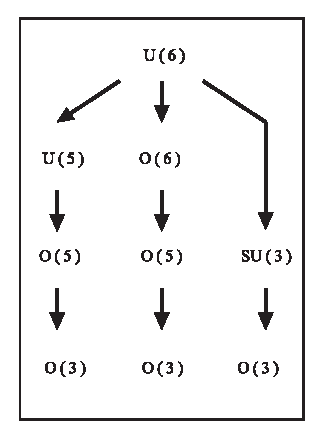
\includegraphics[height=4cm]{figure.eps}
%
% If not, use
%\picplace{5cm}{2cm} % Give the correct figure height and width in cm
%
\caption{Please write your figure caption here}
\label{fig:1}       % Give a unique label
\end{figure}
%
% For built-in environments use
%
\begin{theorem}
Theorem text goes here.
\end{theorem}
%
% or
%
\begin{lemma}
Lemma text goes here.
\end{lemma}
%
%
% Problems or Exercises should be sorted chapterwise
\section*{Problems}
\addcontentsline{toc}{section}{Problems}
%
% Use the following environment.
% Don't forget to label each problem;
% the label is needed for the solutions' environment
\begin{prob}
\label{prob1}
The problem\footnote{Footnote} is described here. The
problem is described here. The problem is described here.
\end{prob}

\begin{prob}
\label{prob2}
\textbf{Problem Heading}\\
(a) The first part of the problem is described here.\\
(b) The second part of the problem is described here.
\end{prob}



%

%\appendix
%\documentclass[12pt]{article}
\usepackage{amsmath}
\usepackage{enumitem}
\usepackage{fixmath}
\usepackage{amsfonts}
\usepackage{graphicx}
\usepackage{xcolor}
\definecolor{colorsrc}{rgb}{0.36, 0.54, 0.66}

% \definecolor{colornan}{rgb}{0.5, 0.5, 0.5}
% \definecolor{colornan}{rgb}{0.43, 0.21, 0.1}
% \definecolor{auburn}{rgb}{0.43, 0.21, 0.1}
% \definecolor{colorwnd2}{rgb}{1, .44, .37}
\definecolor{colorlcksvd}{rgb}{0.91, 0.84, 0.42}
\definecolor{colorlcksvdd}{rgb}{0.8, 0.0, 0.1}
\definecolor{colorlcksvd}{rgb}{1, 0.56, 0.0}
% \definecolor{colornan}{rgb}{0, 0.8, 0.0}
% \definecolor{colorsrc}{rgb}{0.5, 1, 0}
% \definecolor{colorfdd}{rgb}{0.6, 0.4, 0.8}
% \definecolor{colorfdd}{rgb}{0.93, 0.53, 0.18}
\definecolor{colorfddl}{rgb}{0.44, 0.16, 0.39}
\definecolor{colordlsi}{rgb}{0.55, 0.71, 0.0}
% \definecolor{colorlck}{rgb}{0.43, 0.21, 0.1}
% \definecolor{colorlck}{rgb}{0.89, 0.82, 0.04}
% \definecolor{colorlck}{rgb}{0.03, 0.27, 0.49}
\definecolor{colorcopar}{rgb}{0.9, .0, 0}
% \definecolor{colorlrsd}{rgb}{0.72, 0.53, 0.04}
\definecolor{colorjdl}{rgb}{0.0, 0.55, 0.55}
\definecolor{colordlr}{rgb}{0.0, 0.55, 0.55}
\definecolor{colorlrsdl}{rgb}{0.0, 0.2, 1.0} % blue
% \definecolor{colorlck}{rgb}{0.5, 0.5, 0.0}
% \definecolor{colorlck}{rgb}{0.0, 0.42, 0.24}
\definecolor{colorlck}{rgb}{0.0, 0.9, 0.9}
\definecolor{pinegreen}{rgb}{0.0, 0.47, 0.44}

\def\myaddplotlrsdl{\addplot+[thick, colorlrsdl, solid, mark = square*, mark size=1.4, mark options={colorlrsdl}]}
\def\myaddplotfddl{\addplot+[thick, colorfddl, mark = diamond*, mark size=1.4, mark options={colorfddl}]}
\def\myaddplotlcksvd{\addplot+[thick, colorlcksvd, mark = x, mark size=1.8, mark options={colorlcksvd}]}
\def\myaddplotlcksvdd{\addplot+[thick, green, mark = triangle, mark size=1.4, mark options={green}]}
\def\myaddplotdlsi{\addplot+[thick, colordlsi, mark = *, mark size=1.4, mark options={fill = white}]}
\def\myaddplotsrc{\addplot+[thick, colorsrc, mark = square, mark size=1.4, mark options={colorsrc}]}
\def\myaddplotcopar{\addplot+[thick, colorcopar, solid, mark = *, mark size=1.4, mark options={colorcopar}]}
\def\myaddplotjdl{\addplot+[thick, pinegreen, solid, mark = diamond*, mark size=1.4, mark options={pinegreen}]}
\def\myaddplotdlr{\addplot+[thick, cyan, solid, dashed, mark = triangle*, mark size=1.4, mark options={cyan}]}


% \def\myaddplotcopar{\addplot+[colorcopar, mark = square*, mark options={colorcopar}]}
% \def\myaddplotdfd{\addplot+[colordfd,  mark options={colordfd}]}
% \def\myaddplotfdd{\addplot+[colorfdd,  mark options={colorfdd}]}
% \def\myaddplotlck{\addplot+[colorlck,  mark options={colorlck}]}
% \def\myaddplotnan{\addplot+[colornan,  mark options={colornan}]}
% \def\myaddplotwnd{\addplot+[colorwnd,  mark options={colorwnd}]}
% \def\wnd{{black,fill=colorwnd}}

\def\x{{\mathbf x}}
\def\L{{\cal L}}

\newcommand{\vect}[1]{\mathbf{#1}}

\newcommand{\mat}[1]{\mathbf{#1}}
\newcommand{\abs}[1]{\left|#1\right|}
\newcommand{\norm}[1]{\left\|#1\right\|}
% \newcommand{\R}{\mathbb{R}}
\newcommand{\Z}{\mathbb{Z}}
\newcommand{\tb}{\textbf}


\def\bmt{\left[\begin{matrix}}
\def\dpcm{$\square$}
\def\emt{\end{matrix}\right]}
% \def\proof{\underline{Proof:}\\}
\def\dpcm{$\square$}
\def\half{\frac{1}{2}}
\def\imply{\Rightarrow}
\def\foralli{\forall i = 1, 2, \dots, n}
\def\im{\mathrm{im}}
\def\ker{\mathrm{ker}}
\def\eqv{\Leftrightarrow}
\def\tcg{\textcolor{newgreen}}
\def\mb{\mathbf}
\def\tb{\textbf}
\def\mb {\mathbf}
\def\mc {\mathcal}
\def\tcb{\textcolor{blue}}
\def\tcg{\textcolor{green}}
\def\tcr{\textcolor{red}}
\def\tcgr{\textcolor{gray}}
\def\bx{\mathbf{x}}
% \def\bW{\mathbf{W}}
\def\ba{\mathbf{a}}
\def\bb{\mathbf{b}}
\def\bc{\mathbf{c}}
\def\bd{\mathbf{d}}
\def\be{\mathbf{e}}
\def\fb{\mathbf{f}}
\def\bg{\mathbf{g}}
\def\bh{\mathbf{h}}
\def\bm{\mathbf{m}}
\def\M{\mathcal{M}}
\def\bp{\mathbf{p}}
\def\bq{\mathbf{q}}
\def\bs{\mathbf{x}}
\def\bu{\mathbf{u}}
\def\bv{\mathbf{v}}
\def\by{\mathbf{y}}
\def\bz{\mathbf{z}}
\def\and{\text{~and~}}
\def\barN{\bar{N}}
\def\barNi{\bar{N}_i}
\def\trace{\textrm{trace}}
\def\etal{\textit{et al.}}
\def\R{\mathbb{R}}

\def\bzeros{\mathbf{0}}

\def\bA{\mathbf{A}}
\def\bB{\mathbf{B}}
\def\bD{\mathbf{D}}
\def\bE{\mathbf{E}}
\def\Fb{\mathbf{F}}
\def\bG{\mathbf{G}}
\def\bL{\mathbf{L}}
\def\bH{\mathbf{H}}
\def\bI{\mathbf{I}}
\def\bJ{\mathbf{J}}
\def\bM{\mathbf{M}}
\def\bN{\mathbf{N}}
\def\bP{\mathbf{P}}
\def\bQ{\mathbf{Q}}
\def\bR{\mathbf{R}}
\def\bS{\mathbf{S}}
\def\bU{\mathbf{U}}
\def\bV{\mathbf{V}}
\def\bW{\mathbf{W}}
\def\bX{\mathbf{X}}

\def\bY{\mathbf{Y}}
\def\bZ{\mathbf{Z}}
\def\rank{\text{rank}}
\def\bDi{\mathbf{D}_i}
% \def\bSi{\mathbf{X}_i}
\def\bXi{\mathbf{X}_i}
% \def\bSi{\mathbf{X}_i}
\def\barX{\bar{\mathbf{X}}}
\def\barD{\bar{\mathbf{D}}}
\def\barX{\bar{\mathbf{X}}}
\def\barXi{\bar{\mathbf{X}}_i}
\def\barDi{\bar{\mathbf{D}}_i}
\def\barXi{\bar{\mathbf{X}}_i}
\def\bW{\mathbf{W}}
\def\bw{\mathbf{w}}

\def\la{\langle}
\def\ra{\rangle}

\def\bDc{\bD_{0}}
\def\bXc{\bX^{0}}
\def\mM{\mathcal{M}}
\def\wt{\widetilde}

\def\bbX{\lbar{\bX}}        
\def\bbx{\lbar{\bx}}        
\def\bbY{\lbar{\bY}}        
\def\bbD{\lbar{\bD}}  

%% ================== block: Slide footnotes ==========================
\def\footnoteSRC{\setcounter{footnote}{3}\footnote[frame]{\tiny J. Wright et al., Robust face recognition via sparse representation, IEEE TPAMI, 2009}}
\def\footnoteLLC{\setcounter{footnote}{4}\footnote[frame]{\tiny  H. Zhang et. al., Locality-constrained linear coding for image classification, CPVR 2010}}
\def\footnoteJSRC{\setcounter{footnote}{5}\footnote[frame]{\tiny  Yen, Multi-View Automatic Target Recognition using Joint Sparse Representation, Aerospace and Electronic Sys. 2012}}
\def\footnoteJDSRC{\setcounter{footnote}{6}\footnote[frame]{\tiny  J. Wang et. al., Joint dynamic sparse representation for multi-view face recognition,  PR 2012}}
\def\footnoteSHIRC{\setcounter{footnote}{7}\footnote[frame]{\tiny U. Srinivas et. al., Simultaneous sparsity model for histopathological image representation and classification, TMI 2014}}
\def\footnoteKSVD{\setcounter{footnote}{8}\footnote[frame]{\tiny  M. Elad et. al., K -SVD: An Algorithm for Designing Overcomplete Dictionaries for Sparse Representation, TSP 2006 }}
\def\footnoteODL{\setcounter{footnote}{9}\footnote[frame]{\tiny J. Mairal et. al., Online learning for matrix factorization and sparse coding, JMLR 2010}}
\def\footnoteDKSVD{\setcounter{footnote}{10}\footnote[frame]{\tiny  Q. Zhang, B. Li, Discriminative K-SVD for dictionary learning in face recognition, CVPR 2010 }}

\def\footnoteLCKSVD{\setcounter{footnote}{11}\footnote[frame]{\tiny  Z. Jiang et. al., Label consistent K-SVD: Learning a discriminative dictionary for recognition, TPAMI 2013}}
\def\footnoteFDDL{\setcounter{footnote}{12}\footnote[frame]{\tiny  M. Yang et. al., Fisher discrimination dictionary learning for sparse representation, ICCV 2011, IJCV 2014 }}
\def\footnoteDLR{\setcounter{footnote}{20}\footnote[frame]{\tiny  L. Li et. al., Learning low-rank and discriminative dictionary for image classification, Image and Vision Computing, 2014}}
\def\footnoteOMP{\setcounter{footnote}{13}\footnote[frame]{\tiny  Tropp et. al., Signal recovery from random measurements via orthogonal matching pursuit,  IEEE Transactions on Information Theory 2007}}
\def\footnoteNANDITA{\setcounter{footnote}{14}\footnote[frame]{\tiny N. Nayak et. al., Classification of tumor histopathology via sparse feature learning, ISBI 2013}}
\def\footnoteWNDCHARM{\setcounter{footnote}{15}\footnote[frame]{\tiny L. Shamir et. al., WNDCHARM--an open source utility for biological image analysis,  Source Code Biol. Med., 2008}}

\def\footnoteDFDLTMI{\setcounter{footnote}{16}\footnote[frame]{\tiny  \tcr{T. Vu} et. al., Histopathological Image Classification using Discriminative Feature-oriented Dictionary Learning, TMI 2015}}
\def\footnoteADMM{\setcounter{footnote}{17}\footnote[frame]{\tiny S. Boyd et. al., Distributed Optimization and Statistical Learning via the Alternating Direction Method of Multipliers, Foundations and Trends in Machine Learning, 2011}}
\def\footnoteFISTA{\setcounter{footnote}{18}\footnote[frame]{\tiny A. Beck et. al., A fast iterative shrinkage-thresholding algorithm for linear inverse problems, SIAM journal on Imaging sciences, 2009}}
\def\footnoteHojjatJPI{\setcounter{footnote}{19}\footnote[frame]{\tiny H. Mousavi \etal, Automated discrimination of lower and higher grade gliomas based on histopathological image analysis, JPI, 2015}}
% \def\footnote
% \def\footnoteDLSI{\setcounter{footnote}{3}\footnote[frame]{\tiny  I. Ramirez et. al., IEEE Computer Vision and Pattern Recognition (CVPR), 2010 }}






\def\footnotea{\setcounter{footnote}{3}\footnote[frame]{\tiny  H. Chang et. al., IEEE Transactions on Medical Imaging (TMI), 2013}}
\def\footnoteb{\setcounter{footnote}{4}\footnote[frame]{\tiny E. Ozdemir et. al., IEEE Transactions on Medical Imaging (TMI), 2013}}
\def\footnotec{\setcounter{footnote}{5}\footnote[frame]{\tiny M. Murat Dundar et. al., IEEE Transactions on Biomedical Engineering (TBME), 2011}}

\def\footnoteGDDL{\setcounter{footnote}{21}\footnote[frame]{\tiny  Suo et. al., Structured dictionary learning for classification, submitted to TSP 2014}}
\def\footnoteDLCORPA{\setcounter{footnote}{22}\footnote[frame]{\tiny S. Kong et. al., ECCV 2012}}
\def\footnoteDDLPC{\setcounter{footnote}{23}\footnote[frame]{\tiny  Guo et. al., ACCV 2012}}
\def\footnoteLPDDL{\setcounter{footnote}{24}\footnote[frame]{\tiny  Haghiri et. al., ICIP 2014}}
\def\footnoteDLSI{\setcounter{footnote}{25}\footnote[frame]{\tiny  Ramirez et. al., Classification and clustering via dictionary learning with structured incoherence and shared features, CVPR 2010}}
\def\footnoteDFDL{\setcounter{footnote}{26}\footnote[frame]{\tiny  T. Vu et. al., ISBI 2015}}
\def\footnoteDLRDSR{\setcounter{footnote}{27}\footnote[frame]{\tiny L. Ma et. al., CVPR 2012}}
\def\footnoteTDDL{\setcounter{footnote}{28}\footnote[frame]{\tiny J. Mairal et. al., ``Task-driven dictionary learning'', TPAMI, 2012}}
\def\footnoteTDDLLP{\setcounter{footnote}{29}\footnote[frame]{\tiny X. Sun, N. Nasrabadi, T. Tran, ``Task-driven dictionary learning for hyperspectral image classification with structured sparsity constraints'', TGRS, 2015}}
\def\footnoteJohn{\setcounter{footnote}{30}\footnote[frame]{\tiny J. Mckay, V. Monga \etal, Pose corrected sparsity for robust SONAR ATR, IGRSS, 2016}}



\def\diag{\text{diag}}


%% ------------------end of block: Slide footnotes ----------------------------



\newcommand{\myFormA}[1]{\bmt #1 & \bzeros & \dots & \bzeros \\ \bzeros & #1 & \dots & \bzeros \\ \dots & \dots & \dots & \dots \\ \bzeros & \bzeros & \dots & #1  \emt}
\newcommand{\myFormB}[1]{\bmt #1 & #1 & \dots & #1 \\ #1 & #1 & \dots & #1 \\ \dots & \dots & \dots & \dots \\ #1 & #1 & \dots & #1  \emt}

        
%% ========= long bar notation ==============================
\makeatletter
\newsavebox\myboxA
\newsavebox\myboxB
\newlength\mylenA
\newcommand*\lbar[2][.75]{%
    \sbox{\myboxA}{$\m@th#2$}%
    \setbox\myboxB\null% Phantom box
    \ht\myboxB=\ht\myboxA%
    \dp\myboxB=\dp\myboxA%
    \wd\myboxB=#1\wd\myboxA% Scale phantom
    \sbox\myboxB{$\m@th\overline{\copy\myboxB}$}%  Overlined phantom
    \setlength\mylenA{\the\wd\myboxA}%   calc width diff
    \addtolength\mylenA{-\the\wd\myboxB}%
    \ifdim\wd\myboxB<\wd\myboxA%
       \rlap{\hskip 0.5\mylenA\usebox\myboxB}{\usebox\myboxA}%
    \else
        \hskip -0.3\mylenA\rlap{\usebox\myboxA}{\hskip 0.3\mylenA\usebox\myboxB}%
    \fi}
\makeatother

\def\lbD{\lbar{\bD}}
\def\lbY{\lbar{\bY}}
\def\lbX{\lbar{\bX}}
% \def\lbX{\overline{\mathbf{X}}}
% \def\lbY{\overline{\mathbf{Y}}}
\usepackage{multirow}
\usepackage[margin=1in]{geometry} 

\usepackage[T5]{fontenc}

\usepackage[utf8]{inputenc}

\usepackage{setspace}
\setstretch{1} 
\setlength{\parskip}{1em}
\setlength{\parindent}{0em} 

\usepackage{algorithmicx}
\usepackage[ruled]{algorithm}
\usepackage{algpseudocode}
\alglanguage{pseudocode}
\usepackage{hyperref}

\def\mF{\mathcal{F}_S}

\usepackage{amssymb}

% \renewcommand{\qedsymbol}{\rule{0.7em}{0.7em}}

\begin{document}
 \begin{center}
  \textbf{\Huge Ôn tập Đại số tuyến tính}\\ 
  \vspace{.25cm}
\small{\bf Theo blog: \url{http://machinelearningcoban.com}
}\\
\vspace{.5cm}
  Vũ Hữu Tiệp, 2017
\end{center}

%!TEX root = appendix.tex
% \chapter{Convex sets và convex functions}
% --- 
 
% Một số kiến thức về Đại Số Tuyến Tính, Xác Suất Thống Kê, Toán Tối Ưu cần thiết cho Machine Learning. 
 
% (\textit{đang trong thời gian xây dựng, cập nhật theo bài}) 

\section{Lưu ý về ký hiệu}
 
Trong các bài viết của tôi, các số vô hướng được biểu diễn bởi các chữ cái viết ở dạng không in đậm, có thể viết hoa, ví dụ $x_1, N, y, k$. Các vector được biểu diễn bằng các chữ cái thường in đậm, ví dụ $\mathbf{y}, \mathbf{x}_1 $. Nếu không giải thích gì thêm, các vector được mặc định hiểu là các vector cột. Các ma trận được biểu diễn bởi các chữ viết hoa in đậm, ví dụ $\mathbf{X, Y, W} $. 
 
Đối với vector, $\mathbf{x} = [x_1, x_2, \dots, x_n]$ được hiểu là một vector hàng. Trong khi $\mathbf{x} = [x_1; x_2; \dots; x_n] $ được hiểu là vector cột. Chú ý sự khác nhau giữa dầu phẩy ($,$) và dấu chấm phẩy ($;$). Đây chính là ký hiệu được Matlab sử dụng. 
 
Tương tự, trong ma trận, $\mathbf{X} = [\mathbf{x}_1, \mathbf{x}_2, \dots, \mathbf{x}_n]$ được hiểu là các vector cột $\mathbf{x}_j$ được đặt cạnh nhau theo thứ tự từ trái qua phải để tạo ra ma trận $\mathbf{X}$. Trong khi $\mathbf{X} = [\mathbf{x}_1; \mathbf{x}_2; \dots; \mathbf{x}_m]$ được hiểu là các vector $\mathbf{x}_i$ được đặt chồng lên nhau theo thứ tự từ trên xuống dưới dể tạo ra ma trận $\mathbf{X}$. Các vector được ngầm hiểu là có kích thước phù hợp để có thể xếp cạnh hoặc xếp chồng lên nhau. 
 
Cho một ma trận $\mathbf{W}$, nếu không giải thích gì thêm, chúng ta hiểu rằng $\mathbf{w}_i$ là \textbf{vector cột} thứ $i$ của ma trận đó. Chú ý sự tương ứng giữa ký tự viết hoa và viết thường. 
 
 
\section{Norms (chuẩn)}
Trong không gian một chiều, việc đo khoảng cách giữa hai điểm đã rất quen thuộc: lấy trị tuyệt đối của hiệu giữa hai giá trị đó. Trong không gian hai chiều, tức mặt phẳng, chúng ta thường dùng khoảng cách Eclid để đo khoảng cách giữa hai điểm. Khoảng cách này chính là cái chúng ta thường nói bằng ngôn ngữ thông thường là \textit{đường chim bay}. Đôi khi, để đi từ một điểm này tới một điểm kia, con người chúng ta không thể đi bằng đường chim bay được mà còn phụ thuộc vào việc đường đi nối giữa hai điểm có dạng như thế nào nữa.  
 
Việc đo khoảng cách giữa hai điểm dữ liệu nhiều chiều, tức hai vector, là rất cần thiết trong Machine Learning. Chúng ta cần đánh giá xem điểm nào là điểm gần nhất của một điểm khác; chúng ta cũng cần đánh giá xem độ chính xác của việc ước lượng; và trong rất nhiều ví dụ khác nữa.  
 
Và đó chính là lý do mà khái niệm norm (chuẩn) ra đời. Có nhiều loại norm khác nhau mà các bạn sẽ thấy ở dưới đây:  
 
Để xác định khoảng cách giữa hai vector $\mathbf{y}$ và $\mathbf{z}$, người ta thường áp dụng một hàm số lên vector hiệu $\mathbf{x = y - z}$. Một hàm số được dùng để đo các vector cần có một vài tính chất đặc biệt.  
 
\subsection{Định nghĩa}
Một hàm số $f() $ ánh xạ một điểm $\mathbf{x}$ từ không gian $n$ chiều sang tập số thực một chiều được gọi là norm nếu nó thỏa mãn ba điều kiện sau đây: 
 
\begin{enumerate}

	\item $f(\mathbf{x}) \geq 0$. Dấu bằng xảy ra $\Leftrightarrow \mathbf{x = 0} $.

	\item $f(\alpha \mathbf{x}) = \|\alpha\| f(\mathbf{x}), ~~~\forall \alpha \in \mathbb{R}\ $

	\item $f(\mathbf{x}_1) + f(\mathbf{x}_2) \geq f(\mathbf{x}_1 + \mathbf{x}_2), ~~\forall \mathbf{x}_1, \mathbf{x}_2 \in \mathbf{R}^n$
\end{enumerate}
 
\textbf{Điều kiện thứ nhất} là dễ hiểu vì khoảng cách không thể là một số âm. Hơn nữa, khoảng cách giữa hai điểm $\mathbf{y}$ và $\mathbf{z}$ bằng 0 nếu và chỉ nếu hai điểm nó trùng nhau, tức $\mathbf{x = y - z = 0} $. 
 
\textbf{Điều kiện thứ hai} cũng có thể được lý giải như sau. Nếu ba điểm $\mathbf{y, v}$ và $\mathbf{z}$ thẳng hàng, hơn nữa $\mathbf{v - y} = \alpha (\mathbf{v - z}) $ thì khoảng cách giữa $\mathbf{v}$ và $\mathbf{y}$ sẽ gấp $ \|\alpha \|$ lần khoảng cách giữa $\mathbf{v}$ và $\mathbf{z}$. 
 
\textbf{Điều kiện thứ ba} chính là bất đẳng thức tam giác nếu ta coi $\mathbf{x}_1 = \mathbf{ w - y}, \mathbf{x}_2 = \mathbf{z - w} $ với $\mathbf{w}$ là một điểm bất kỳ trong cùng không gian. 
 
 
 
\subsection{Một số chuẩn thường dùng}
 
Giả sử các vectors $\mathbf{x} = [x_1; x_2; \dots; x_n]$, $\mathbf{y} = [y_1; y_2; \dots; y_n]$. 
 
Nhận thấy rằng khoảng cách Euclid chính là một norm, norm này thường được gọi là \textbf{norm 2}: 
\begin{equation} 
	\label{eqn:norm2}
	\|\mathbf{x}\|_2 = \sqrt{x_1^2 + x_2^2 + \dots x_n^2} 
\end{equation}
 
Với $p$ \textbf{là một số không nhỏ hơn 1} bất kỳ, hàm số sau đây: 
\begin{equation} 
	\label{eqn:normp}
	\|\mathbf{x}\|_p = (\|x_1\|^p + \|x_2\|^p + \dots \|x_n\|^p)^{\frac{1}{p}} 
\end{equation} 
 
được chứng minh thỏa mãn ba điều kiện bên trên, và được gọi là \textbf{norm p}.  
     	
 
Nhận thấy rằng khi $p \rightarrow 0 $ thì biểu thức bên trên trở thành \textit{số các phần tử khác 0 của} $\mathbf{x}$. Hàm số \eqref{eqn:normp} khi $p = 0$ được gọi là giả chuẩn (pseudo-norm) 0. Nó không phải là norm vì nó không thỏa mãn điều kiện 2 và 3 của norm. Giả-chuẩn này, thường được ký hiệu là $\|\mathbf{x}\|_0$, khá quan trọng trong Machine Learning vì trong nhiều bài toán, chúng ta cần có ràng buộc “sparse”, tức số lượng thành phần “active” của $\mathbf{x}$ là nhỏ.  
 
Có một vài giá trị của $p$ thường được dùng: 

\begin{enumerate}
 	\item Khi $p = 2$ chúng ta có norm 2 như ở trên.
 
 	
 	\item Khi $p = 1$ chúng ta có:
		\begin{equation} 
		\label{eqn:norm1}
		\|\mathbf{x}\|_1 = \|x_1\| + \|x_2\| + \dots \|x_n\|
		\end{equation} 
		là tổng các trị tuyệt đối của từng phần tử của $\mathbf{x}$. Norm 1 thường được dùng như xấp xỉ của norm 0 trong các bài toán có ràng buộc "sparse". Dưới đây là một ví dụ so sánh norm 1 và norm 2 trong không gian hai chiều: 

		\begin{figure}
			\centering	
			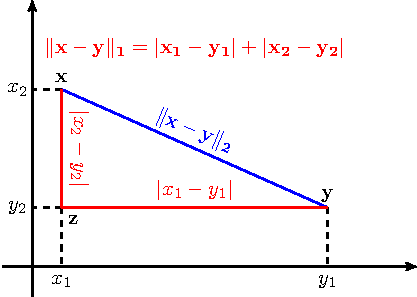
\includegraphics[width = .5\textwidth]{norm12.pdf}
			\caption{Minh họa norm 1 và norm 2}
			\label{fig:norm12}
		\end{figure}
		Norm 2 (màu xanh) chính là đường thằng "chim bay" nối giữa hai vector $\mathbf{x} $ và $\mathbf{y}$. Khoảng cách norm 1 giữa hai điểm này (màu đỏ) có thể diễn giải như là đường đi từ $\mathbf{x} $ tới $\mathbf{y}$ trong một thành phố mà đường phố tạo thành hình bàn cờ. Chúng ta chỉ có cách đi dọc theo cạnh của bàn cờ mà không được đi thẳng. 
 	
 	\item Khi $p \rightarrow \infty $, ta có norm $p$ chính là trị tuyệt đối của phần tử lớn nhất của vector đó:
		\begin{equation} 
		\|\mathbf{x}\|_{\infty} = \max_{i = 1, 2, \dots, n} \|x_i\|
		\end{equation} 
 
\end{enumerate} 
 
\subsection{Chuẩn của ma trận}
Với một ma trận $\mathbf{A} \in \mathbb{R}^{m\times n}$, chuẩn thường được dùng nhất là chuẩn Frobenius, ký hiệu là $\|\mathbf{A}\|_F$ là căn bậc hai của tổng bình phương tất cả các phần tử của ma trận đó.  
\begin{equation*} 
\|\mathbf{A}\|_F = \sqrt{\sum_{i = 1}^m \sum_{j = 1}^n a_{ij}^2} 
\end{equation*} 
 
 
 
 
\section{Đạo hàm của hàm nhiều biến }
Trong mục này, chúng ta sẽ giả sử rằng các đạo hàm tồn tại. Chúng ta sẽ xét hai trường hợp: i) Hàm số nhận giá trị là ma trận (vector) và cho giá trị là một số thực vô hướng; và ii) Hàm số nhận giá trị là một số vô hướng hoặc vector và cho giá trị là một vector.  
 
 
\subsection{Hàm cho giá trị là một số vô hướng}
 
Đạo hàm (gradient) của một hàm số $f(\mathbf{x}): \mathbb{R}^n \rightarrow \mathbb{R}$ \textbf{theo vector} $\mathbf{x}$ được định nghĩa như sau:  
 
\begin{equation} 
	\label{eqn:grvector1}
	\nabla_{\mathbf{x}} f(\mathbf{x}) \triangleq  
	\left[ 
	\begin{matrix} 
	\frac{\partial f(\mathbf{x})}{\partial x_1} \\\ 
	\frac{\partial f(\mathbf{x})}{\partial x_2} \\\ 
	\vdots \\\ 
	\frac{\partial f(\mathbf{x})}{\partial x_n} 
	\end{matrix} 
	\right] \in \mathbb{R}^n 
\end{equation} 
trong đó $\frac{\partial f(\mathbf{x})}{\partial x_i}$ là đạo hàm của hàm số theo thành phần thứ $i$ của vector $\mathbf{x}$. Đạo hàm này được lấy khi giả sử tất cả các biến còn lại là hằng số. 
 
Nếu không có thêm biến nào trong hàm số, $\nabla_{\mathbf{x}}f(\mathbf{x})$ thường được viết gọn là $\nabla f(\mathbf{x})$. 
 
Điều quan trọng cần nhớ: \textbf{đạo hàm của hàm số này là một vector có cùng chiều với vector đang lấy đạo hàm}. Tức nếu vector viết ở dạng cột thì đạo hàm cũng phải viết ở dạng cột.  
 
Đạo hàm bậc hai (second-order gradient) của hàm số trên còn được gọi là \textit{Hessian} và được định nghĩa như sau:  
 
\begin{equation} 
\label{eqn:hessian1}
\nabla^2 f(\mathbf{x}) \triangleq 
\left[ 
\begin{matrix} 
    \frac{\partial^2 f(\mathbf{x})}{\partial x_1^2} & \frac{\partial^2 f(\mathbf{x})}{\partial x_1x_2} & \dots & \frac{\partial^2 f(\mathbf{x})}{\partial x_1x_n} \\\  
    \frac{\partial^2 f(\mathbf{x})}{\partial x_2x_1} & \frac{\partial^2 f(\mathbf{x})}{\partial x_2^2} & \dots & \frac{\partial^2 f(\mathbf{x})}{\partial x_2x_n} \\\  
    \vdots & \vdots & \ddots & \vdots \\\ 
    \frac{\partial^2 f(\mathbf{x})}{\partial x_nx_1} & \frac{\partial^2 f(\mathbf{x})}{\partial x_nx_2} & \dots & \frac{\partial^2 f(\mathbf{x})}{\partial x_n^2} \\\  
\end{matrix} 
\right] \in \mathbb{S}^{n}
\end{equation}  
với $\mathbb{S}^{n} \in \mathbb{R}^{n \times n}$ là tập các ma trận vuông đối xứng có số cột là $n$. 

Đạo hàm của một hàm số $f(\mathbf{X}): \mathbb{R}^{n \times m} \rightarrow \mathbb{R}$ \textbf{theo ma trận} $\mathbf{X}$ được định nghĩa là:  
\begin{equation}
\label{eqn:grmatrix1} 
\nabla f(\mathbf{X}) = 
\left[ 
\begin{matrix} 
    \frac{\partial f(\mathbf{X})}{\partial x_{11}} & \frac{\partial f(\mathbf{X})}{\partial x_{12}} & \dots & \frac{\partial f(\mathbf{X})}{\partial x_{1m}} \\\ 
    \frac{\partial f(\mathbf{X})}{\partial x_{21}} & \frac{\partial f(\mathbf{X})}{\partial x_{22}} & \dots & \frac{\partial f(\mathbf{X})}{\partial x_{2m}} \\\ 
    \vdots & \vdots & \ddots & \vdots \\\ 
    \frac{\partial f(\mathbf{X})}{\partial x_{n1}} & \frac{\partial f(\mathbf{X})}{\partial x_{n2}} & \dots & \frac{\partial f(\mathbf{X})}{\partial x_{nm}}  
\end{matrix} 
\right] \in \mathbb{R}^{n \times m}
\end{equation} 
 
Một lần nữa, đạo hàm của một hàm số theo ma trận là một ma trận có chiều giống với ma trận đó. 
 
Hiểu một cách đơn giản, đạo hàm của một hàm số (có đầu ra là 1 số vô hướng) theo một ma trận được tính như sau. Trước tiên, tính đạo hàm của hàm số đó theo từng thành phần của ma trận \textit{khi toàn bộ các thành phần khác được giả sử là hằng số}. Tiếp theo, ta \textit{ghép} các đạo hàm thành phần tính được thành một ma trận đúng theo thứ tự như trong ma trận đó. Chú ý rằng vector là một trường hợp của ma trận.  
 
\textbf{Ví dụ:} Xét hàm số: $f: \mathbb{R}^2 \rightarrow \mathbb{R}$, $f(\mathbf{x}) = x_1 ^2 + 2x_1x_2 + \sin(x_1) + 2$.  
 
Đạo hàm bậc nhất theo $\mathbf{x}$ của hàm số đó là:  
\begin{equation*} 
\nabla f(\mathbf{x}) = 
\left[ 
\begin{matrix} 
    \frac{\partial f(\mathbf{x})}{\partial x_1} \\\ 
    \frac{\partial f(\mathbf{x})}{\partial x_2} 
\end{matrix} 
\right] = \left[ 
\begin{matrix} 
    2x_1 + 2x_2 + \cos(x_1) \\\ 
    2x_1 
\end{matrix} 
\right] 
\end{equation*} 
 
Đạo hàm bậc hai theo $\mathbf{x}$, hay \textit{Hessian} là:  
\begin{equation*} 
\nabla^2 f(\mathbf{x}) =  
\left[ 
\begin{matrix} 
    \frac{\partial^2 f(\mathbf{x})}{\partial x_1^2} & \frac{\partial f^2(\mathbf{x})}{\partial x_1x_2} \\\ 
    \frac{\partial^2 f(\mathbf{x})}{\partial x_2x_1} & \frac{\partial f^2(\mathbf{x})}{\partial x_2^2} 
\end{matrix} 
\right] = 
\left[ 
\begin{matrix} 
    2 - \sin(x_1) & 2 \\\ 
    2 & 0  
\end{matrix} 
\right] 
\end{equation*} 
Chú ý rằng \textit{Hessian} luôn là một ma trận đối xứng.  
 
 
 
\subsection{Hàm cho giá trị là một vector }
 
Những hàm số cho giá trị là một vector được gọi là \textit{vector-valued function} trong tiếng Anh.  
 
Giả sử một hàm số với \textbf{đầu vào là một số thực} $v(x): \mathbb{R} \rightarrow \mathbb{R}^n $: 
\begin{equation} 
\label{eqn:vectorvalued}
v(x) =  
\left[ 
\begin{matrix} 
    v_1(x) \\\ 
    v_2(x) \\\ 
    \vdots \\\ 
    v_n(x) 
\end{matrix} 
\right] 
\end{equation} 
Đạo hàm của nó là một \textbf{vector hàng} như sau:  

\begin{equation} 
\label{eqn:grvectorvalued}
\nabla v(x) \triangleq  
\left[ 
\begin{matrix} 
    \frac{\partial v_1(x)}{\partial x} & \frac{\partial v_2(x)}{\partial x} & \dots & \frac{\partial v_n(x)}{\partial x} 
\end{matrix} 
\right]
\end{equation} 
Đạo hàm bậc hai của hàm số này có dạng: 
 
\begin{equation} 
	\label{eqn:hessianvectorvalued}
	\nabla^2 v(x) \triangleq  
	\left[ 
	\begin{matrix} 
	    \frac{\partial^2 v_1(x)}{\partial x^2} & \frac{\partial^2 v_2(x)}{\partial x^2} & \dots & \frac{\partial^2 v_n(x)}{\partial x^2} 
	\end{matrix} 
	\right] 
\end{equation} 
 
\textbf{Ví dụ:} Cho vector $\mathbf{a} \in \mathbb{R}^n$ và \textit{vector-valued function} $v(x) = x\mathbf{a}$, thế thì: 
\begin{equation} 
\nabla v(x) = \mathbf{a}^T, ~~~ \nabla^2 v(x) = \mathbf{0} \in \mathbb{R}^{n\times n} 
\end{equation} 
với $\mathbf{0}$ là ma trận với các thành phần đều là 0.  

Xét một \textit{vector-valued function} với \textbf{đầu vào là một vector} $h(\mathbf{x}):\mathbb{R}^k \rightarrow \mathbb{R}^n$, đạo hàm bậc nhất của nó là: 
\begin{eqnarray} 
\label{eqn:gdvectorvector}
\nabla h(\mathbf{x}) &\triangleq & 
\left[ 
\begin{matrix} 
    \frac{\partial h_1(\mathbf{x})}{\partial x_1} & \frac{\partial h_2(\mathbf{x})}{\partial x_1} & \dots & \frac{\partial h_n(\mathbf{x})}{\partial x_1} \\\  
    \frac{\partial h_1(\mathbf{x})}{\partial x_2} & \frac{\partial h_2(\mathbf{x})}{\partial x_2} & \dots & \frac{\partial h_n(\mathbf{x})}{\partial x_2} \\\  
    \vdots & \vdots & \ddots & \vdots \\\ 
    \frac{\partial h_1(\mathbf{x})}{\partial x_k} & \frac{\partial h_2(\mathbf{x})}{\partial x_k} & \dots & \frac{\partial h_n(\mathbf{x})}{\partial x_k} 
\end{matrix} 
\right]\\
\label{eqn:gdvectorvector_short}
& = &  
\left[ 
\begin{matrix} 
    \nabla h_1(\mathbf{x}) & \nabla h_2(\mathbf{x}) & \dots & \nabla h_n(\mathbf{x}) 
\end{matrix} 
\right] \in \mathbf{R}^{k\times n} 
\end{eqnarray} 
 
 
\textbf{Một quy tắc dễ nhớ ở đây là nếu một hàm số} $g: \mathbb{R}^m \rightarrow \mathbb{R}^n$ \textbf{thì đạo hàm của nó là một ma trận thuộc} $\mathbb{R}^{m \times n}$. 
 
Đạo hàm bậc hai của hàm số trên là một \textit{ma trận ba chiều}, tôi xin không đề cập ở đây.  
 

<hr> 
Với các hàm số \textit{matrix-valued} nhận giá trị đầu vào là ma trận, tôi cũng xin không đề cập ở đây. Tuy nhiên, ở phần dưới, khi tính toán đạo hàm cho các hàm cho giá trị là số thực, chúng ta vẫn có thể sẽ sử dụng khái niệm này. 
 
Trước khi đến phần tính đạo hàm của các hàm số thường gặp, chúng ta cần biết hai tính chất quan trọng khá giống với đạo hàm của hàm một biến được học trong chương trình cấp ba.  
 
 
\subsection{Hai tính chất quan trọng }
 
 
\subsubsection{Product rules}
Để cho tổng quát, ta giả sử biến đầu vào là một ma trận (vector và số thực là các trường hợp đặt biệt của ma trận). Giả sử rằng các hàm số có chiều phù hợp để các phép nhân thực hiện được. Ta có:  
 
\begin{equation} 
\label{eqn:productrules}
\nabla\left( f(\mathbf{X})^Tg(\mathbf{X}) \right) = \left(\nabla f(\mathbf{X})\right) g(\mathbf{X}) + \left(\nabla g(\mathbf{X})\right) f(\mathbf{X})  
\end{equation} 
 
Biểu thức này giống như biểu thức chúng ta đã quá quen thuộc: 
\begin{equation*} 
\left(f(x)g(x)\right)' = f'(x)g(x) + g'(x)f(x) 
\end{equation*} 
Chú ý rằng với vector và ma trận, chúng ta không được sử dụng tính chất giao hoán.  
 
 
\subsubsection{Chain rules }
Khi có các hàm hợp thì: 
\begin{equation} 
\label{eqn:chainrules}
\nabla_{\mathbf{X}} g(f(\mathbf{X})) = \nabla_{\mathbf{X}} f^T \nabla_{f}g ~~~ (15) 
\end{equation} 
 
Quy tắc này cũng giống với quy tắc trong hàm một biến:  
\begin{equation*} 
(g(f(x))' = f'(x)g'(f) 
\end{equation*} 
Nhắc lại rằng khi tính toán với ma trận, chúng ta cần chú ý tới chiều của các ma trận, và nhân ma trận không có tính chất giao hoán.  
 
\subsection{Đạo hàm của các hàm số thường gặp }
 
\subsubsection{$f(\mathbf{x}) = \mathbf{a}^T\mathbf{x}$}
 
Giả sử $\mathbf{a}, \mathbf{x} \in \mathbb{R}^n$, ta viết lại: 
\begin{equation*} 
f(\mathbf{x}) = \mathbf{a}^T\mathbf{x} = a_1 x_1 + a_2 x_2 + \dots + a_nx_n 
\end{equation*} 
Có thể nhận thấy rằng: 
\begin{equation*} 
\frac{\partial f(\mathbf{x})}{\partial x_i} = a_i, ~ \forall i = 1, 2\dots, n 
\end{equation*} 
Vậy nên: 
\begin{equation*} 
\nabla f(\mathbf{x}) =  
\left[ 
\begin{matrix} 
    a_1 \\\ 
    a_2 \\\ 
    \vdots \\\ 
    a_n 
\end{matrix} 
\right] = \mathbf{a}
\end{equation*} 
 
Thêm nữa, vì $\mathbf{a}^T\mathbf{x} = \mathbf{x}^T\mathbf{a}$ nên: 
\begin{equation*} 
\nabla (\mathbf{x}^T\mathbf{a}) = \mathbf{a} 
\end{equation*} 
 
 
\subsubsection{$f(\mathbf{x}) = \mathbf{Ax}$}
Đây là một \textit{vector-valued function} $f: \mathbb{R}^n \rightarrow \mathbb{R}^{m} $ với $\mathbf{x} \in \mathbb{R}^n, \mathbf{A} \in \mathbb{R}^{m\times n}$. Giả sử rằng $\mathbf{a}_i$ là \textbf{hàng} thứ $i$ của ma trận $\mathbf{A}$. Ta có:  
\begin{equation*} 
\mathbf{Ax}  =  
\left[ 
\begin{matrix} 
    \mathbf{a}_1\mathbf{x} \\\ 
    \mathbf{a}_2\mathbf{x} \\\ 
    \vdots\\\ 
    \mathbf{a}_m\mathbf{x}  
\end{matrix} 
\right] 
\end{equation*} 
Theo định nghĩa $(13.2)$, và công thức $(17)$, ta có thể suy ra: 
\begin{equation} 
\label{eqn:gdAx}
\nabla_{\mathbf{x}} (\mathbf{Ax}) =  
\left[ 
\begin{matrix} 
    \mathbf{a}_1^T & \mathbf{a}_2^T & \dots & \mathbf{a}_m^T 
\end{matrix} 
\right] = \mathbf{A}^T 
\end{equation} 
 
Từ đây ta có thể suy ra đạo hàm của hàm số $f(\mathbf{x}) = \mathbf{x} = \mathbf{Ix}$, với $\mathbf{I}$ là ma trận đơn vị với chiều phù hợp, là: 
\begin{equation*} 
\nabla \mathbf{x} = \mathbf{I} 
\end{equation*} 
 
\subsubsection{$f(\mathbf{x}) = \mathbf{x}^T\mathbf{A} \mathbf{x}$}
với $\mathbf{x} \in \mathbb{R}^n, \mathbf{A} \in \mathbb{R}^{n\times n}$. Áp dụng Product rules $(14)$ ta có: 
\begin{eqnarray} 
	\nonumber
	\nabla f(\mathbf{x}) &=& \nabla \left(\left(\mathbf{x}^T\right) \left(\mathbf{Ax}\right)\right) \\\ 
				\nonumber
                     &=& \left(\nabla (\mathbf{x})\right) \mathbf{Ax} + \left(\nabla (\mathbf{Ax})\right)\mathbf{x} \\\  
					\nonumber
                     & = & \mathbf{IAx} + \mathbf{A}^T\mathbf{x} \\\ 
                     \label{eqn:gdxTAx}
                     & = & (\mathbf{A} + \mathbf{A}^T)\mathbf{x} 
\end{eqnarray} 
 
 
Từ \eqref{eqn:gdxTAx} và \eqref{eqn:gdAx}, ta có thể suy ra:  
\begin{math} 
\nabla^2 \mathbf{x}^T\mathbf{Ax} = \mathbf{A}^T + \mathbf{A} 
\end{math} 
 
Nếu $\mathbf{A}$ là một ma trận đối xứng, ta sẽ có: 
\begin{equation} 
\nabla \mathbf{x}^T\mathbf{A}\mathbf{x} = 2\mathbf{Ax}, ~~~
\nabla^2 \mathbf{x}^T\mathbf{Ax} = 2\mathbf{A} 
\end{equation} 
 
Nếu $\mathbf{A}$ là ma trận đơn vị, tức $f(\mathbf{x}) = \mathbf{x}^T\mathbf{Ix} = \mathbf{x}^T\mathbf{x} = \|\mathbf{x}\|_2^2$, ta có: 
\begin{equation} 
\nabla \|\mathbf{x}\|_2^2 = 2\mathbf{x},~~~
\nabla^2 \|\mathbf{x}\|_2^2 = 2\mathbf{I} 
\end{equation} 
 
 
\subsubsection{$f(\mathbf{x}) = \|\mathbf{Ax} - \mathbf{b}\|_2^2 $}
Có hai cách tính đạo hàm của hàm số này: 
 
\textbf{Cách 1:} 
Trước hết, biến đổi: 
\begin{eqnarray} 
	\nonumber
	f(\mathbf{x}) &=& \|\mathbf{Ax} - \mathbf{b}\|_2^2 = (\mathbf{Ax} - \mathbf{b})^T(\mathbf{Ax} - \mathbf{b}) = (\mathbf{x}^T\mathbf{A}^T - \mathbf{b}^T) (\mathbf{Ax} - \mathbf{b}) \\\ \nonumber
	&=& \mathbf{x}^T\mathbf{A}^T\mathbf{Ax} - 2 \mathbf{b}^T\mathbf{Ax} + \mathbf{b}^T\mathbf{b} 
\end{eqnarray} 
Lấy đạo hàm cho từng số hạng rồi cộng lại ta có:  
\begin{equation*} 
\nabla \|\mathbf{Ax} - \mathbf{b}\|_2^2 = 2\mathbf{A}^T\mathbf{A}\mathbf{x} - 2\mathbf{A}^T\mathbf{b} = 2\mathbf{A}^T(\mathbf{Ax} - \mathbf{b}) 
\end{equation*} 
 
\textbf{Cách 2:} Dùng Chain rule. 
Sử dụng $\nabla (\mathbf{Ax} - \mathbf{b}) = \mathbf{A}^T$ và $\nabla \|\mathbf{x}\|_2^2 = 2\mathbf{x}$ và công thức chain rules \eqref{eqn:chainrules}, ta sẽ thu được kết quả tương tự.  
 
 
\subsubsection{$f(\mathbf{x}) = \mathbf{a}^T\mathbf{x}\mathbf{x}^T\mathbf{b}$}
Bằng cách viết lại $f(\mathbf{x}) = (\mathbf{a}^T\mathbf{x})(\mathbf{x}^T\mathbf{b})$, ta có thể dùng Product rules $(14)$ và ra kết quả:  
\begin{equation*} 
	\nabla (\mathbf{a}^T\mathbf{x}\mathbf{x}^T\mathbf{b}) = \mathbf{a} \mathbf{x}^T\mathbf{b} +  \mathbf{b}\mathbf{a}^T\mathbf{x} = \mathbf{ab}^T\mathbf{x} + \mathbf{b}\mathbf{a}^T\mathbf{x}= (\mathbf{ab}^T + \mathbf{ba}^T)\mathbf{x} 
\end{equation*} 
trong đây tôi đã sử dụng tính chất $\mathbf{y}^T\mathbf{z} = \mathbf{z}^T\mathbf{y}$ và tích của một số thực với một vector cũng bằng tích của vector và số thực đó.  
 
 
\subsection{Bảng các đạo hàm thường gặp}
 
\subsubsection{Cho vector }
 
\begin{table}[h!]
\centering
\caption{Đạo hàm theo vector}
\label{my-label}
\begin{tabular}{|c|c|}
\hline
$f(\mathbf{x}) $                                                                          & $ \nabla f(\mathbf{x}) $                                         \\ \hline
$\mathbf{a}^T \mathbf{x} $                                                                & $\mathbf{a}$                                                     \\ \hline
$\mathbf{x}^T\mathbf{Ax}$                                                                 & $\mathbf{A} + \mathbf{A}^T) \mathbf{x}$                          \\ \hline
$\mathbf{x}^T \mathbf{x} = \|\mathbf{x}\|_2^2 $ & $2\mathbf{x}$                                                   \\ \hline
$ \|\mathbf{Ax-b} \|_2^2 $                                                                & $ 2\mathbf{A}^T (\mathbf{Ax - b})$                               \\ \hline
$\mathbf{a}^T\mathbf{x}^T\mathbf{xb} $                                                    & $2\mathbf{a}^T\mathbf{bx} $                                      \\ \hline
$\mathbf{a}^T\mathbf{x}\mathbf{x}^T\mathbf{b} $                                           & $ (\mathbf{a}\mathbf{b}^T + \mathbf{b}\mathbf{a}^T) \mathbf{x} $ \\ \hline
\end{tabular}
\end{table}


 
\subsubsection{Cho ma trận}
 

 \begin{table}[h!]
\centering
\caption{Đạo hàm theo ma trận}
\label{my-label}
\begin{tabular}{|c|c|}
\hline
$f(\mathbf{X}) $                                   & $ \nabla f(\mathbf{X}) $                      \\ \hline
$ \|\mathbf{X}\|_F^2$ & $2\mathbf{X}$ \\\hline
$ \mathbf{AX}$ & $\mathbf{A}^T$ \\\hline
$ \|\mathbf{AX - B}\|_F^2$ & $2\mathbf{A}^T(\mathbf{AX - B})$ \\\hline
$ \|\mathbf{XA - B}\|_F^2$ & $2(\mathbf{XA-B})\mathbf{A}^T$ \\\hline
$ \mathbf{a}^T \mathbf{X}^T \mathbf{Xb}$           & $ \mathbf{X}(\mathbf{ab}^T + \mathbf{ba}^T)$ \\ \hline
$ \mathbf{a}^T \mathbf{X} \mathbf{X}^T \mathbf{b}$ & $ (\mathbf{ab}^T + \mathbf{ba}^T)\mathbf{X},$ \\ \hline
$ \mathbf{a}^T \mathbf{Y} \mathbf{X}^T \mathbf{b}$ & $ \mathbf{b}\mathbf{a}^T \mathbf{Y}$         \\ \hline
$ \mathbf{a}^T \mathbf{Y}^T \mathbf{X} \mathbf{b}$ & $ \mathbf{Y}\mathbf{a}\mathbf{b}^T$          \\ \hline
$ \mathbf{a}^T \mathbf{X} \mathbf{Y}^T \mathbf{b}$ & $ \mathbf{a}\mathbf{b}^T\mathbf{Y}$          \\ \hline
$ \mathbf{a}^T \mathbf{X}^T \mathbf{Y} \mathbf{b}$ & $ \mathbf{Y}\mathbf{b}\mathbf{a}^T$          \\ \hline
\end{tabular}
\end{table}


\subsection{Tài liệu tham khảo }
[1] \href{https://ccrma.stanford.edu/~dattorro/matrixcalc.pdf}{Matrix calculus} 
 
 
 

\end{document}

\backmatter%%%%%%%%%%%%%%%%%%%%%%%%%%%%%%%%%%%%%%%%%%%%%%%%%%%%%%%
% 
\chapter*{Solutions}
\addcontentsline{toc}{chapter}{Solutions}
\markboth{Solutions}{Solutions}

\section*{Problems of Chapter~\ref{intro}}

\begin{sol}{prob1}
The solution is revealed here.
\end{sol}


\begin{sol}{prob2}
\textbf{Problem Heading}\\
(a) The solution of first part is revealed here.\\
(b) The solution of second part is revealed here.
\end{sol}


% %%%%%%%%%%%%%%%%%%%%%%%% referenc.tex %%%%%%%%%%%%%%%%%%%%%%%%%%%%%%
% sample references
% "computer science"
%
% Use this file as a template for your own input.
%
%%%%%%%%%%%%%%%%%%%%%%%% Springer-Verlag %%%%%%%%%%%%%%%%%%%%%%%%%%

%
% BibTeX users please use
% \bibliographystyle{}
% \bibliography{}
%
% Non-BibTeX users please use
\begin{thebibliography}{99.}
%
% and use \bibitem to create references.
%
% Use the following syntax and markup for your references
%
% Monographs
\bibitem{monograph} Kajan E (2002)
Information technology encyclopedia and acronyms. Springer, Berlin
Heidelberg New York

% Contributed Works
\bibitem{contribution} Broy M (2002) Software engineering -- From
auxiliary to key technologies. In: Broy M, Denert E (eds)
Software Pioneers. Springer, Berlin Heidelberg New York

% Journal
\bibitem{journal} Che M, Grellmann W, Seidler S (1997)
Appl Polym Sci 64:1079--1090

% Theses
\bibitem{thesis} Ross DW (1977) Lysosomes and storage diseases. MA
Thesis, Columbia University, New York

\end{thebibliography}

\printindex

%%%%%%%%%%%%%%%%%%%%%%%%%%%%%%%%%%%%%%%%%%%%%%%%%%%%%%%%%%%%%%%%%%%%%%

\end{document}
